\PassOptionsToPackage{quiet}{fontspec}
\documentclass{article}

%%%%%%%%%%%%%%%%%%% usepackage %%%%%%%%%%%%%%%%%%%

\usepackage[a4paper, margin=1in]{geometry}
\usepackage{ctex}

% paragraph
\usepackage{parskip}
% math
\usepackage{amsthm}
\usepackage{amsfonts}
\usepackage{amsmath}
\usepackage{amssymb}
\usepackage{mathtools}
\usepackage{centernot}
\usepackage{arydshln}
\setcounter{MaxMatrixCols}{11}
% reference
\usepackage[hidelinks]{hyperref}
% layout
\usepackage{booktabs}
\usepackage{graphicx}
\usepackage{setspace}
\usepackage{framed}
\usepackage{float}
% color and box
\usepackage{xcolor}
\usepackage{tcolorbox}
\tcbuselibrary{breakable}
% table
\usepackage{multicol}
\usepackage{multirow}
% list
\usepackage{enumitem}
\setlist{noitemsep}
% font
\usepackage{fontspec}
\setmainfont{TeX Gyre Termes}


%%%%%%%%%%%%%%%%%%%%%% math %%%%%%%%%%%%%%%%%%%%%%

\theoremstyle{definition}
\newtheorem{theorem}{定理}[section]
\newtheorem{corollary}[theorem]{推论}
\newtheorem{lemma}[theorem]{引理}
\newtheorem*{property}{性质}

\theoremstyle{definition}
\newtheorem{definition}{定义}[section]
\newtheorem{example}{例}[section]
\newtheorem{exercise}{练习}

\theoremstyle{remark}
\newtheorem*{remark}{注解}
\newtheorem*{note}{注意}
\newtheorem*{com}{注释}

\tcolorboxenvironment{example}{colback=blue!5!white, boxrule=0.5pt, breakable}
\tcolorboxenvironment{remark}{colback=green!10!white, boxrule=0.5pt, breakable}
\tcolorboxenvironment{note}{colback=yellow!10!white, boxrule=0.5pt, breakable}
\tcolorboxenvironment{proof}{colback=black!5!white, boxrule=0.5pt, breakable}


%%%%%%%%%%%%%%%%%% new command %%%%%%%%%%%%%%%%%%%
\newcommand{\ind}{\mathrel{\perp\!\!\!\!\perp}}
\newcommand{\Cov}{\mathrm{Cov}}
\newcommand{\Var}{\mathrm{Var}}
\newcommand{\E}{\mathbb{E}}
\newcommand{\G}{\mathbb{G}}
\newcommand{\V}{\mathbb{V}}
\newcommand{\Pb}{\mathbb{P}}
\newcommand{\sigmaXX}{\sigma_{\scalebox{.6}{$XX$}}}
\newcommand{\sigmaYY}{\sigma_{\scalebox{.6}{$YY$}}}
\newcommand{\sigmaXY}{\sigma_{\scalebox{.6}{$XY$}}}
\newcommand{\sigmaYX}{\sigma_{\scalebox{.6}{$YX$}}}
\newcommand{\sigmaXYZ}{\sigma_{\scalebox{.6}{$XY\vert Z$}}}
\newcommand{\sigmaYXZ}{\sigma_{\scalebox{.6}{$YX\vert Z$}}}
\newcommand{\pa}{\mathrm{pa}}
\newcommand{\ch}{\mathrm{ch}}
\newcommand{\nb}{\mathrm{nb}}
\newcommand{\bd}{\mathrm{bd}}
\newcommand{\cl}{\mathrm{cl}}
\newcommand\norm[1]{\Vert#1\Vert}


%%%%%%%%%%%%%%%%%%%%%% main %%%%%%%%%%%%%%%%%%%%%%

\begin{document}

\begin{titlepage}
    \vspace*{0.5cm}
    \begin{center}
        \rule{\linewidth}{2.0pt} \\[\baselineskip]
        {\LARGE \textbf{\uppercase{Lecture Notes}}}\\[0.8\baselineskip]
        {\Large {Matrix Analysis and Applications}}\\[0.2\baselineskip]
        \rule{\linewidth}{1.5pt} \\
        
        \vfill
        \begin{figure}[H]
            \centering
            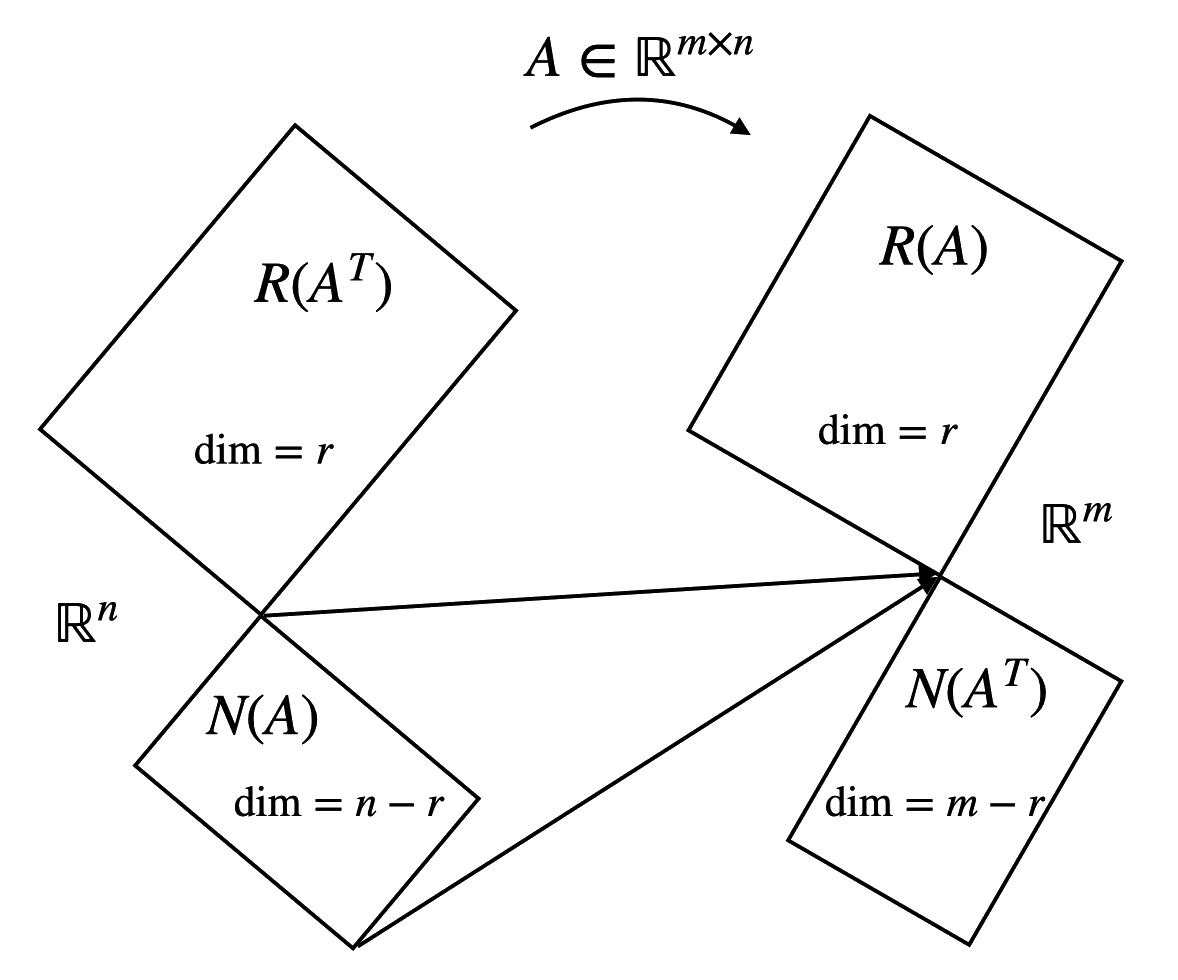
\includegraphics[width=0.6\linewidth]{figs/space.png}
        \end{figure}
        \vfill
        
        {\large \textbf{Yifeng Xu}\\University of Chinese Academy of Sciences}\\[0.5cm]
        {\large 2023.09 -- 2024.01}
    \end{center}
\end{titlepage}

\thispagestyle{empty}
\newpage

\nocite{*}
\textbf{Course}

Matrix Analysis and Applications

\vspace{2ex}

\textbf{School}

University of Chinese Academy of Sciences

\vspace{2ex}

\textbf{Lecturer}

Prof. Shiwei Ye

\vspace{2ex}

\textbf{Textbook}

程云鹏, 张凯院, 徐仲. 矩阵论（第3版）

\newpage
\section*{前言}

这是一篇关于《矩阵论》课程的笔记。该课程由中国科学院大学电子电气与通信工程学院开设，所用教材为程云鹏等人编著的《矩阵论》\cite{cheng2006matrix}，因此本笔记大致按照该书章节顺序安排。作为面向工科生的数学课程，该书涉及内容多但又不够深入，缺乏对相关概念的解释与引导，有堆砌定义定理之嫌。因此，本笔记将尽力穿插一些解释性语句，补充一些注解，必要时重新安排定义定理的引出顺序，希望能梳理出自然的思考逻辑。其他参考资料包括张贤达《矩阵分析与应用》\cite{zhang2004matrix}、Axler《线性代数应该这样学》\cite{axler2015linear}和 Horn 等人《矩阵分析》\cite{horn2012matrix}.
 \newpage
\tableofcontents \newpage
\section{线性空间和线性映射}

\subsection{线性空间}

% \begin{definition}[映射，变换，函数]
% 设有集合 $S,S'$，定义规则 $\sigma:S\to S'$，使得集合 $S$ 中元素 $a$ 与 $S'$ 中唯一元素对应，记作：
% \[
%     a'=\sigma(a)\quad\text{或}\quad \sigma:a\mapsto a'
% \]
% 则称 $\sigma$ 为一个映射。特别地，若 $S$ 与 $S'$ 相同，则称 $\sigma$ 为变换；若 $S'$ 为数域，则称 $\sigma$ 为函数。
% \end{definition}
% \begin{com}
% 映射最本质的特征在于对于 $S$ 中的任意一个元素在 $S'$ 中仅有唯一的一个元素和它对应。
% \end{com}

% \begin{definition}[集值映射]
% 由单点映射 $\sigma:S\to S'$ 可导出集值映射 $\sigma:2^S\to 2^{S'}$，
% \begin{align*}
%     \sigma(\Omega)&=\{y:y=\sigma(x),\exists\,x\in\Omega\},\quad\forall\,\Omega\subset S\\
%     \sigma^{-1}(\Omega')&=\{x:y=\sigma(x),\exists\,y\in\Omega'\},\quad\forall\,\Omega'\subset S'
% \end{align*}
% 如图所示：
% \begin{figure}[H]
%     \centering
%     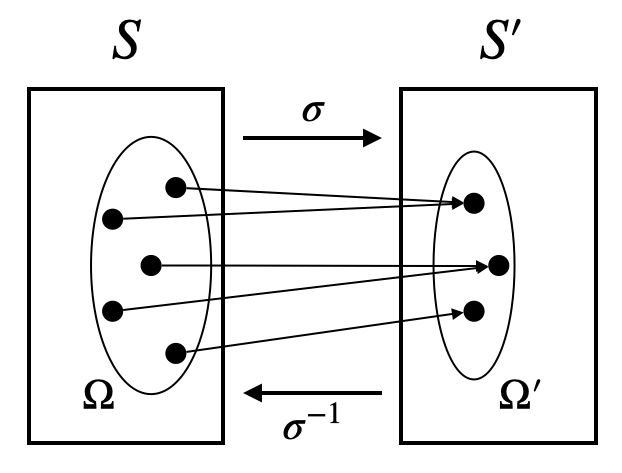
\includegraphics[width=0.25\linewidth]{figs/set-proj.png}
% \end{figure}

% \end{definition}

% \begin{property}[集值映射的基本性质]
% 集值映射满足如下基本性质：
% \begin{itemize}
%     \item 任给子集 $\Omega\subset S$，则 $\sigma^{-1}(\sigma(\Omega))=\Omega$.
%     \item 任给子集 $\Omega'\subset S'$，则 $\sigma(\sigma^{-1}(\Omega'))=\Omega'\cap \sigma(S)$.
% \end{itemize}
% 如果用包含关系定义子集间的偏序关系，那么由映射导出的集值映射是保持这种偏序关系的，即：
% \begin{align*}
% &\Omega_1\subset\Omega_2\subset S\implies \sigma(\Omega_1)\subset \sigma(\Omega_2)\subset \sigma(S)\\
% &\Omega'_1\subset\Omega'_2\subset S\implies \sigma^{-1}(\Omega'_1)\subset \sigma^{-1}(\Omega'_2)\subset \sigma^{-1}(S)
% \end{align*}
% \end{property}

\begin{definition}[线性空间/向量空间]
设 $V$ 是一个非空集合，它的元素用 $x,y,z$ 等表示，称为向量；$\mathbb F$ 是一个数域（$\mathbb R$ 或 $\mathbb C$），它的元素用 $k,l$ 等表示，称为标量。定义加法与数乘：
\begin{gather*}
    +:V\times V\to V,\;(x,y)\mapsto x+y\\
    \cdot:\mathbb F\times V\to V,\;(k,x)\mapsto k\cdot x
\end{gather*}
如果加法和数乘满足下列 8 条性质：
\begin{itemize}
    \item 结合律：$x+(y+z)=(x+y)+z$
    \item 交换律：$x+y=y+x$
    \item 存在零元素：$x+0=x$
    \item 存在负元素：$x+(-x)=0$
    \item 数因子分配律：$k(x+y)=kx+ky$
    \item 分配律：$(k+l)x=kx+lx$
    \item 结合律：$k(lx)=(kl)x$
    \item 存在单位元：$1x=x$
\end{itemize}
则称 $(V,\mathbb F,+,\cdot)$ 为数域 $\mathbb F$ 上的线性空间或向量空间，简记作 $V$. 特别地，当 $\mathbb F$ 为实数域 $\mathbb R$ 时，称之为实线性空间；当 $\mathbb F$ 为复数域 $\mathbb C$ 时，称之为复线性空间。
\end{definition}

\begin{remark}
集合中的元素无需一定是列向量，可以是矩阵、多项式等；加法和数乘也不一定是我们熟悉的加法和数乘，只要满足上述 8 条性质即可。因此线性空间是多种多样的。
\end{remark}

\begin{example}
\label{ex:linearspace-pn}
次数不超过$n−1$的多项式$P_n$全体按照通常的多项式加法和数乘构成一个线性的多项式函数空间。
\end{example}

\begin{example}
\label{ex:linearspace-rn}
$n$ 维实列向量的全体按照通常的向量加法和实数域上的数乘构成一个实线性空间，称为实向量空间，记作 $\mathbb R^n$.
\end{example}

\begin{example}
\label{ex:linearspace-cn}
$n$ 维复列向量的全体按照通常的向量加法和复数域上的数乘构成一个复线性空间，称为复向量空间，记作 $\mathbb C^n$.
\end{example}

\begin{example}
\label{ex:linearspace-cnr}
$n$ 维复列向量的全体按照通常的向量加法和\textbf{实数域}上的数乘构成一个线性空间。
\end{example}

\begin{note}
注意例 \ref{ex:linearspace-cn} 与例 \ref{ex:linearspace-cnr} 唯一的区别是数域不同，但这就会导致二者的结构不同。
\end{note}

\begin{example}
所有 $m\times n$ 实矩阵的全体按照通常的矩阵加法和数乘构成一个实线性空间，称为矩阵空间。
\end{example}

\begin{example}
\label{ex:linearspace}
取 $V=\mathbb R^n$，对 $x,y\in V,\,k\in\mathbb R$，定义加法 $\oplus$ 和数乘 $\odot$：
\begin{align*}
    &x\oplus y=\left((x_1^3+y_1^3)^{1/3},(x_2^3+y_2^3)^{1/3}\ldots,(x_n^3+y_n^3)^{1/3}\right)^T\\
    &k\odot x=k^{1/3}x
\end{align*}
则 $(\mathbb R^n,\mathbb R,\oplus,\odot)$ 构成一个线性空间。
\end{example}

\begin{example}
\label{ex:linearspace2}
取 $V=\mathbb R^+$，对 $x,y\in V,\,k\in\mathbb R$，定义加法 $\oplus$ 和数乘 $\odot$：
\begin{align*}
    &x\oplus y=x\cdot y\\
    &k\odot x=x^k
\end{align*}
则 $(\mathbb R^+,\mathbb R,\oplus,\odot)$ 构成一个线性空间。
\end{example}

\begin{definition}[线性相关，线性无关]
若存在一组不全为零的数$c_1,c_2,\ldots,c_m$，使得：
\[
    c_1x_1+c_2x_2+\cdots+c_mx_m=0
\]
则称向量组$x_1,x_2,\ldots,x_m$线性相关，否则称为线性无关。
\end{definition}

\begin{definition}[线性表示]
若向量 $x$ 可以表示为向量组 $x_1,x_2,\ldots,x_m$ 的线性组合，即存在一组系数 $c_1,c_2,\ldots,c_m$ 使得：
\[
    x=c_1x_1+c_2x_2+\cdots c_mx_m
\]
则称 $x$ 可以由向量组 $x_1,x_2,\ldots,x_m$ 线性表示，相应 $c_1,c_2,\ldots,c_m$ 称作表示系数。
\end{definition}

\begin{theorem}
\label{thm:linear-repre-only}
设向量 $x$ 可以由 $x_1,x_2,\ldots,x_m$ 线性表示，若 $x_1,x_2,\ldots,x_m$ 线性无关，则表示系数唯一。
\end{theorem}
\begin{proof}
设存在另一组表示系数 $d_1,d_2,\ldots,d_m$，则：
\[
    x=c_1x_1+c_2x_2+\cdots+c_mx_m=d_1x_1+d_2x_2+\cdots+d_mx_m
\]
于是：
\[
    (c_1-d_1)x_1+(c_2-d_2)x_2+\cdots+(c_m-d_m)x_m=0
\]
由于 $x_1,x_2,\ldots,x_m$ 线性无关，故 $c_i=d_i,\,i=1,2,\ldots,m$.
\end{proof}

为书写方便，将 $x_1,x_2,\ldots,x_m$ 并排放在一起写作 $X=(x_1,x_2,\ldots,x_m)$，将表示系数排成列向量的形式 $c=(c_1,c_2,\ldots,c_m)^T$，则 $x=c_1x_1+c_2x_2+\cdots+c_mx_m$ 可简便记作：
\[
    x=(x_1,x_2,\ldots,x_m)c\quad\text{或}\quad x=Xc
\]
注意，这里 $X$ 表示向量组而非矩阵，$Xc$ 也并非矩阵乘法，应按照线性表示来理解。
进一步，假若向量组 $y_1,y_2,\ldots,y_n$ 中的每一个向量都可以由 $x_1,x_2,\ldots,x_m$ 线性表示，即：
\[
    y_j=c_{1j}x_1+c_{2j}x_2+\cdots+c_{mj}x_m,\quad j=1,2,\ldots,n
\]
那么引入记号 $X=(x_1,x_2,\ldots,x_m),\,Y=(y_1,y_2,\ldots,y_n)$，将组合系数排列成一个矩阵 $C=[c_{ij}]$，则上式可以简便记作：
\[
    (y_1,y_2,\ldots,y_n)=(x_1,x_2,\ldots,x_n)C\quad\text{或}\quad Y=XC
\]
同样的，这里 $XC$ 并非矩阵乘法，应按照线性表示理解。

\begin{definition}[极大线性无关组]
若对一个线性无关的向量组，再往里添加向量就无法保持它们的线性无关性，那么称该向量组为极大线性无关组。
\end{definition}

\begin{lemma}
任意线性无关组总是可以扩充为极大线性无关组。
\end{lemma}

\begin{theorem}
\label{thm:maxlinear}
对一个线性空间中的任意两个极大线性无关组，若它们所含向量个数都有限，则所含向量个数一定相同。
\end{theorem}

\begin{proof}
设 $x_1,x_2,\ldots,x_m$ 和 $y_1,y_2,\ldots,y_n$ 为线性空间 $V$ 中的两个极大线性无关组，则它们可以互相线性表示，即存在矩阵 $A,B$ 使得：
\begin{align*}
    &(x_1,x_2,\ldots,x_m)=(y_1,y_2,\ldots,y_n)A\\
    &(y_1,y_2,\ldots,y_n)=(x_1,x_2,\ldots,x_m)B
\end{align*}
联立上述二式得：
\[
    (y_1,y_2,\ldots,y_n)=(y_1,y_2,\ldots,y_n)AB
\]
由于 $y_1,y_2,\ldots,y_n$ 是极大线性无关组，所以只能有 $AB=I_n$，其中 $I_n$ 为 $n$ 阶单位阵，于是：
\[
    \text{tr}(AB)=\text{tr}(I_n)=n
\]
同理可得：
\[
    \text{tr}(BA)=\text{tr}(I_m)=m
\]
根据迹算子的性质，有：
\[
    n=\text{tr}(AB)=\text{tr}(BA)=m
\]
即这两个极大线性无关组所含向量个数相同。
\end{proof}

\begin{definition}[线性空间的维数]
定义线性空间 $V$ 的维数为其中极大线性无关组的所含向量的个数，记作 $\dim V$. 维数有限的称为有限维空间，否则称为无限维空间。
\end{definition}

\begin{com}
这个定义之所以是良定义的，是因为定理 \ref{thm:maxlinear} 说明了有限维空间中，不同极大线性无关组所含向量的个数是相同的。
\end{com}

\begin{example}
考虑全体复数集合 $\mathbb C$，若取数域 $\mathbb F=\mathbb C$，则复数集合对复数加法和复数之间的乘法构成线性空间，其一个极大线性无关组为 $\{1\}$，因此空间维数是 1；但如果取数域 $\mathbb F=\mathbb R$，则复数集合对复数加法和实数与复数之间的数乘构成线性空间，其一个极大线性无关组为 $\{1,i\}$，因此空间维数是 2.
\end{example}

\begin{remark}
本课程只讨论有限维空间，无限维空间属于泛函分析的研究对象。有限维空间下得到的结论有些可以直接推广到无限维空间，有些却不能，必须小心!
\end{remark}

\begin{definition}[基]
若线性空间 $V$ 的向量 $x_1,x_2,\ldots,x_n$ 满足：
\begin{enumerate}
    \item $x_1,x_2,\ldots,x_n$ 线性无关；
    \item $V$ 中任意向量都可由 $x_1,x_2,\ldots,x_n$ 的线性表示。
\end{enumerate}
则称 $x_1,x_2,\ldots,x_r$ 为 $V$ 的一个基或基底，相应地称 $x_i$ 为基向量。
\end{definition}

\begin{corollary}
线性空间中任意一个极大无关组构成它的一个基。
\end{corollary}

\begin{definition}[坐标表示]
设 $X=(x_1,\ldots,x_n)$ 是线性空间 $V$ 的一个基，若向量 $x$ 在这个基下的线性表示为：
\[x=\xi_1 x_1+\cdots+\xi_nx_n=X\xi\]
则称 $x$ 在 $X$ 下的坐标表示为 $\xi=(\xi_1,\ldots,\xi_n)^{T}$.
\end{definition}

\begin{note}
组成基的向量排列是\textbf{有顺序}的！这是因为向量在这个基下的坐标表示是有顺序的，例如 $(1,2)^T\neq (2,1)^T$.
\end{note}

\begin{example}
考虑例 \ref{ex:linearspace-pn} 中介绍的多项式空间 $P_n$，选择 $P_n$ 中的一个基：
\[
    x_1=1,\,x_2=x,x_3=x^2,\ldots,x_n=x^{n-1}
\]
则任意次数不超过 $n-1$ 的多项式 $f(x)=a_0x^{n-1}+a_1x^{n-2}+\cdots+a_{n-2}x+a_{n-1}$ 可写作：
\[
    f(x)=(1,x,x^2,\ldots,x^{n-1})(a_{n-1},a_{n-2},\ldots,a_0)^T
\]
于是 $(a_{n-1},a_{n-2},\ldots,a_0)^T$ 就是多项式 $f(x)$ 在基 $1,x,x^2,\ldots,x^{n-1}$ 下的坐标。
\end{example}

\begin{theorem}[坐标表示构成的映射]
给定线性空间 $V$ 的一个基 $X=(x_1,\ldots,x_n)$，则向量在 $X$ 下的坐标表示定义了从 $V$ 到 $\mathbb R^n$ 或 $\mathbb C^n$ 的一个一一映射：
\[
    \sigma_X: V\to\mathbb R^n (\mathbb C^n),\quad x\mapsto \xi=(\xi_1,\ldots,\xi_n)^T\in\mathbb R^n (\mathbb C^n)
\]
\end{theorem}
\begin{proof}
易证，从略。
\end{proof}

\begin{theorem}
任何 $n$ 维线性空间 $V$ 都与 $\mathbb R^n$ 或 $\mathbb C^n$ 代数同构，即存在一一映射 $\sigma:V\to\mathbb R^n(\mathbb C^n)$ 满足：
\begin{align*}
    &\sigma(x+y)=\sigma(x)+\sigma(y),\quad\forall x,y\in V\\
    &\sigma(kx)=k\sigma(x),\quad\forall x\in V,\,k\in \mathbb F
\end{align*}
\end{theorem}

\begin{proof}
充分性：验证 8 条性质即可；必要性：任给 $V$ 中的一个基，那么该基下的坐标表示就是一个符合条件的同构映射。
\end{proof}

上述定理说明，虽然 $n$ 维线性空间有无穷多，但是\textbf{所有线性空间都与 $\mathbb R^n$ 或 $\mathbb C^n$ 代数同构，因此从代数的角度而言只需研究 $\mathbb R^n$ 和 $\mathbb C^n$ 就足够了}。并且这个同构映射非常简单，就是给定一个基下向量的坐标表示。换句话说，当我们选定一个基之后，不需要去直接研究线性空间的元素本身，而是具体研究它在这个基下的表示系数，这时表示系数本身就属于 $\mathbb R^n$ 或 $\mathbb C^n$，这样我们就可以很直观的了解和分析线性空间的各种结论了。

% 既然如此，为什么我们还要引入抽象的一般化的线性空间的定义呢？这是因为：1.可以把讨论的结论适用于更广的范围；2.由线性映射全体构成的线性空间，可以推广到无限维的线性空间中的线性函数全体构成的线性空间（泛函）；3.利于引进更多的代数运算，如向量的代数乘法，从而引出李代数、结合代数等。

% \begin{example}
% 思考：对于同一个集合 $V$，能否定义不同的加法和数乘使得线性空间 $(V,\mathbb R,\oplus,\odot)$ 和 $(V,\mathbb R,\oplus',\odot')$ 的维数不同？
% 以 $V=[0,1)$ 为例，我们可以定义适当的加法和数乘使得线性空间的维数为 $1,2,\ldots,\infty$，做法如下。考虑在 $[0,1)$ 与 $[0,1)\times[0,1)$ 之间建立一一映射：任给 $x\in[0,1)$，设其二进制小数表示为 $x=0.x_1x_2x_3x_4\ldots$，则定义映射 $\sigma$ 为：
% \[
%     \sigma:x\mapsto y=\begin{bmatrix}y_1\\y_2\end{bmatrix}=\begin{bmatrix}0.x_1x_3\ldots\\0.x_2x_4\ldots\end{bmatrix}
% \]
% 可以验证 $\sigma$ 的确是一一映射。于是对于 $x,y\in[0,1)$，定义加法和数乘为：
% \begin{align*}
%     &\oplus: (x,y)\mapsto x\oplusy=\sigma^{-1}(\sigma(x)+\sigma(y))\\
%     &\odot: (k,x)\mapsto k\odotx=\sigma^{-1}(k\cdot\sigma(k))
% \end{align*}
% 其中 $+$ 和 $\cdot$ 就是 $[0,1)\times[0,1)$ 上常规的向量加法和数乘，那么 $\sigma$ 就是一个同构映射。因此，$([0,1),\mathbb R,\oplus,\odot)$ 就是一个二维的线性空间。（FIXME：数域不太对）
% \end{example}

\begin{definition}[基变换与过渡矩阵]
设有两个基 $X=(x_1,\ldots,x_n)$，$Y=(y_1,\ldots,y_n)$，$Y$ 中每一个基向量由 $X$ 的基向量线性表示为：
\[
    \begin{cases}
    y_1=c_{11}x_1+\cdots+c_{n1}x_n\\
    \quad\vdots\\
    y_n=c_{1n}x_1+\cdots+c_{nn}x_n\\
    \end{cases}
\]
写作矩阵形式为：
\[Y=XC\]
称该式为基变换公式，称 $C$ 为过渡矩阵。
\end{definition}

\begin{corollary}
\label{cor:transmatrix}
过渡矩阵一定非奇异。
\end{corollary}
\begin{proof}
考虑反证法。假设 $C$ 奇异，则存在向量 $\xi\in\mathbb R^n(\mathbb C^n)$ 且 $\xi\neq 0$ 使得 $C\xi=0$. 于是 $Y\xi=XC\xi=0$，即 $\xi_1y_1+\xi_2y_2+\cdots+\xi_ny_n=0$，这与 $Y=(y_1,y_2,\ldots,y_n)$ 是一个基矛盾。
\end{proof}

\begin{com}
从推论 \ref{cor:transmatrix} 我们可以发现，任何一个非奇异矩阵都可以看成是线性空间的两个基之间的过渡矩阵，换句话说，是一个基在另一个基下的坐标表示。
\end{com}

\begin{theorem}[向量在不同基下的坐标表示的关系]
设有一向量 $x$，在两个基下的坐标表示分别为 $\xi=(\xi_1,\ldots,\xi_n)^T$ 和 $\eta=(\eta_1,\ldots,\eta_n)^T$，设 $C$ 为过渡矩阵，则有 $\xi=C\eta$ 或 $\eta=C^{-1}\xi$.
\end{theorem}
\begin{proof}
$x=X\xi=Y\eta\implies\xi=C\eta\iff\eta=C^{-1}\xi$
\end{proof}

\begin{com}
对于 $\mathbb R^n$ 或 $\mathbb C^n$，称 $\{e_1,e_2,\ldots,e_n\}$ 为其\textbf{自然基}，其中 $e_i$ 表示第 $i$ 个分量为 $1$、其余分量为 $0$ 的向量。在自然基下，向量 $x$ 和其坐标表示是一致的，因而常常不加区别地用同一符号表示。
\end{com}

\begin{definition}[线性子空间]
设 $V_1$ 是数域 $\mathbb F$ 上线性空间 $V$ 的非空子集合，且满足：
\begin{enumerate}
    \item 对 $V$ 上的加法封闭：若 $x,y\in V_1$，则 $x+y\in V_1$；
    \item 对 $V$ 上的数乘封闭：若 $x\in V_1,\,k\in \mathbb F$，则 $k\cdot x\in V_1$.
\end{enumerate}
则称 $V_1$ 是 $V$ 的线性子空间或子空间。
\end{definition}

\begin{definition}[零子空间]
称仅由 $0$ 元素构成的子空间为零子空间，其维度为 0.
\end{definition}

\begin{definition}[子空间的和与直和]
设 $V_1,V_2$ 是线性空间 $V$ 的子空间，则它们的和定义为：
\[
    V_1+V_2=\{z\mid z=x+y,\,x\in V_1,\,y\in V_2\}
\]
当 $V_1\cap V_2=\{0\}$ 时，称它们的和为直和，记作 $V_1\oplus V_2$.
\end{definition}

\begin{theorem}
对 $z\in V_1\oplus V_2$，存在唯一的 $x\in V_1,\,y\in V_2$ 使得 $z=x+y$.
\end{theorem}
\begin{proof}
存在性显然，下证唯一性。假设 $z=x_1+y_1=x_2+y_2$，其中 $x_1,x_2\in V_1,\,y_1,y_2\in V_2$，那么 $x_1-x_2=y_2-y_1$. 由于 $x_1-x_2\in V_1,\,y_2-y_1\in V_2$ 且 $V_1\cap V_2=\{0\}$，因此只能是 $x_1=x_2,\,y_1=y_2$.
\end{proof}

% \begin{com}
% 这个性质实际构成了直和定义的背景，也就是说，如果知道 $V_1$ 和 $V_2$，我们可以得到 $V_1+V_2$；但是反过来，如果知道两个子空间 $V_3$ 和 $V_1$，且 $V_1\subset V_3$，我们是否可以知道唯一的子空间 $V_2$，使得 $V_1+V_2=V_3$？直和的定义告诉我们应该如何约束 $V_2$ 以得到唯一性。
% \end{com}

\begin{theorem}
子空间的交仍然是子空间，子空间的和仍然是子空间。
\end{theorem}
\begin{proof}
验证是否对加法和数乘封闭即可，略。
\end{proof}

\begin{theorem}[子空间和的维数公式]
设 $V_1,V_2$ 为线性空间 $V$ 的子空间，则：
\[
    \dim V_1+\dim V_2=\dim (V_1+V_2)+\dim (V_1\cap V_2)
\]    
\end{theorem}

\begin{remark}
\textbf{基扩充}是一种非常重要的证明思路：从最小的子空间 $V_1\cap V_2$ 出发，构造它的一个基 $X=(x_1,\ldots,x_r)$，然后分别扩充成 $V_1$ 的基 $(X,Y)=(x_1,\ldots,x_r,y_1,\ldots,y_s)$ 和 $V_2$ 的基 $(X,Z)=(x_1,\ldots,x_r,z_1,\ldots,z_t)$，最后证明 $(X,Y,Z)=(x_1,\ldots,x_r,y_1,\ldots,y_s,z_1,\ldots,z_t)$ 为 $V_1+V_2$ 的基。    
\end{remark}

\begin{proof}
延续基扩充的证明思路，要证明 $(X,Y,Z)=(x_1,\ldots,x_r,y_1,\ldots,y_s,z_1,\ldots,z_t)$ 为 $V_1+V_2$ 的基，只需证明 1) 线性无关；2) 可线性表示任一 $v\in V_1+V_2$.

1) 首先证明线性无关。设：
\[
    \sum_{i=1}^r a_ix_i+\sum_{j=1}^s b_jy_j+\sum_{k=1}^t c_kz_k=0
\]
则：
\[
    \sum_{i=1}^r a_ix_i+\sum_{j=1}^s b_jy_j=-\sum_{k=1}^t c_kz_k\in V_1
\]
由于 $z_k\notin V_1$，故 $c_k=0$，进而 $a_i=b_j=0$. 故线性无关。

2) 其次，任取 $v\in V_1+V_2$，则 $\exists v_1\in V_1,v_2\in V_2$ 使得 $v_1+v_2=v$. 设：
\[
    v_1=\sum_{i=1}^r a_ix_i+\sum_{j=1}^s c_jy_j,\quad v_2=\sum_{i=1}^r b_ix_i+\sum_{k=1}^t d_kz_k
\]
则：
\[
    v=\sum_{i=1}^r(a_i+b_i)x_i+\sum_{j=1}^s c_jy_j+\sum_{k=1}^t d_kz_k
\]
综上，$(X,Y,Z)$ 是 $V_1+V_2$ 的一个基。    
\end{proof}

\begin{corollary}
设 $V_1,V_2$ 为线性空间 $V$ 的子空间且 $V_1\cap V_2=\{0\}$，则：
\[
    \dim V_1+\dim V_2=\dim (V_1\oplus V_2)
\]
\end{corollary}

\begin{definition}
由向量组张成子空间：
\begin{itemize}
    \item 由单个向量 $x$ 对数乘运算封闭构成一维子空间：$L(x)=\{z\mid z=kx,k\in K\}$；
    \item 由向量组 $x_1,\ldots,x_m$ 张成的子空间：$L(x_1,\ldots,x_m)=L(x_1)+\cdots+L(x_m)$.
\end{itemize}
显然 $\dim L(x_1,\ldots,x_m)\leq m$.    
\end{definition}

通过前面的讨论我们知道了一般的线性空间都和 $\mathbb R^n$ 或 $\mathbb C^n$ 代数同构；另外，$\mathbb R^n$ 或 $\mathbb C^n$ 也是我们最为熟悉的线性空间。因此，我们将它们作为一般线性空间的代表进行讨论与研究，以此来研究抽象的线性空间的性质。为方便起见，下文我们用字母 $\mathbb F$ 表示 $\mathbb R$ 或 $\mathbb C$.

\textbf{$\mathbb F^m$ 空间中的向量组可以用矩阵表示，这在一般的线性空间中是不可行的}。具体而言，矩阵 $A\in\mathbb F^{m\times n}$ 可以看作是 $\mathbb F^m$ 空间中的 $n$ 个向量逐列排列而得；或者换个角度，也可以看作是 $\mathbb F^n$ 空间中的 $m$ 个向量逐行排列而得。采用这种向量组的观点看待矩阵，我们就可以引出矩阵的秩、值域/列空间、核空间/零空间的概念。

\begin{definition}[列秩，行秩]
设 $A\in\mathbb F^{m\times n}$，称其列向量构成的极大线性无关组所包含的向量个数为 $A$ 的列秩，称其行向量构成的极大线性无关组所包含的向量个数为 $A$ 的行秩。
\end{definition}

\begin{theorem}[行秩等于列秩]
设 $A\in\mathbb F^{m\times n}$，则 $A$ 的行秩等于 $A$ 的列秩。
\end{theorem}
\begin{proof}
设 $A$ 的行秩为 $r$，其行向量组构成的一个极大线性无关组为 $(c_1,c_2,\ldots,c_r)$，其中 $c_i$ 为行向量，记矩阵：
\[
    C=\begin{bmatrix}c_1\\c_2\\\vdots\\c_r\end{bmatrix}\in\mathbb F^{r\times n}
\]
则 $A$ 的所有行向量都可以写作 $c_1,c_2,\ldots,c_r$ 的线性组合，用矩阵乘法的记号来表示，即存在矩阵 $B=(b_1,b_2,\ldots,b_r)\in\mathbb F^{m\times r}$，使得：
\[
    A_{m\times n}=B_{m\times r}C_{r\times n}
\]
其中 $B$ 的每一行表示 $A$ 对应行的组合系数。换个角度看待矩阵乘法，上式也意味着 $A$ 的所有列向量都可以写作 $b_1,b_2,\ldots,b_r$ 的线性组合，其中组合系数由 $C$ 的相应列给出。因此 $A \text{ 的列秩} \leq r=A \text{ 的行秩}$. 同理可得 $A \text{ 的行秩}\leq A \text{ 的列秩}$，故行秩等于列秩。
\end{proof}

\begin{definition}[秩]
由于矩阵 $A$ 的列秩与行秩相等，因此统一称作秩，记作 $\text{rank}(A)$.
\end{definition}

\begin{definition}[值域/列空间]
设 $A=(a_1,\ldots,a_n)\in\mathbb F^{m\times n}$，称其列向量张成的子空间 $L(a_1,\ldots,a_n)$ 为矩阵 $A$ 的值域或列空间，记作 $R(A)$，即：
\[
    R(A)=L(a_1,\ldots,a_n)\subset\mathbb F^m
\]
根据定义立刻可知，$\text{rank}(A)=\dim(R(A))$.
\end{definition}

\begin{definition}[核空间/零空间]
设 $A\in\mathbb F^{m\times n}$，称集合 $\{x\mid Ax=0\}$ 为矩阵 $A$ 的核空间或零空间，记作 $N(A)$，即：
\[
    N(A)=\{x\mid Ax=0\}\subset\mathbb F^n
\]
\end{definition}

\begin{theorem}
设 $A\in\mathbb F^{m\times n}$，则 $\dim(R(A))+\dim(N(A))=n$.
\end{theorem}
\begin{proof}
证明思路依旧是\textbf{基扩充}：设 $(x_1,\ldots,x_s)$ 为 $N(A)$ 的一个基，将其扩充为 $\mathbb R^n$ 的基 $(x_1,\ldots,x_s,y_1,\ldots,y_{n-s})$.  只需证明 $(Ay_1,\ldots, Ay_{n-s})$ 是 $R(A)$ 的基。

首先证明线性无关。假设：
\[
    \sum_{j=1}^{n-s}b_j(Ay_j)=0
\]
由于 $Ax_i=0\ (i=1,\ldots,s)$，所以：
\[
    \sum_{j=1}^{n-s}b_jAy_j=\sum_{i=1}^sa_i Ax_i+\sum_{j=1}^{n-s}b_jAy_j=A\left(\sum_{i=1}^sa_i x_i+\sum_{j=1}^{n-s}b_jy_j\right)=0
\]
也就是说：
\[
    \sum_{i=1}^sa_i x_i+\sum_{j=1}^{n-s}b_jy_j\in N(A)
\]
但是 $(x_1,\ldots,x_s)$ 与 $(y_1,\ldots,y_{n-s})$ 是线性无关的，所以只能是 $b_j=0, (j=1,\ldots,n-s)$. 因此线性无关。

其次证明可线性表示。任取 $z\in R(A)$，则存在 $w\in\mathbb R^n$ 使得 $z=Aw$.  设 $w$ 在 $(x_1,\ldots,x_s,y_1,\ldots,y_{n-s})$ 这个基下可以线性表示为：
\[
    w=\sum_{i=1}^s c_ix_i+\sum_{j=1}^{n-s}d_j y_j
\]
那么 $z$ 可以由 $(Ay_1,\ldots,Ay_{n-s})$ 线性表示为：
\[
    z=Aw=\sum_{i=1}^s c_i (Ax_i)+\sum_{j=1}^{n-s}d_j(Ay_j)=\sum_{j=1}^{n-s}d_j(Ay_j)
\]

\end{proof}

\begin{remark}
Gilbert Strang 的著名的四个基本子空间：
\begin{figure}[H]
    \centering
    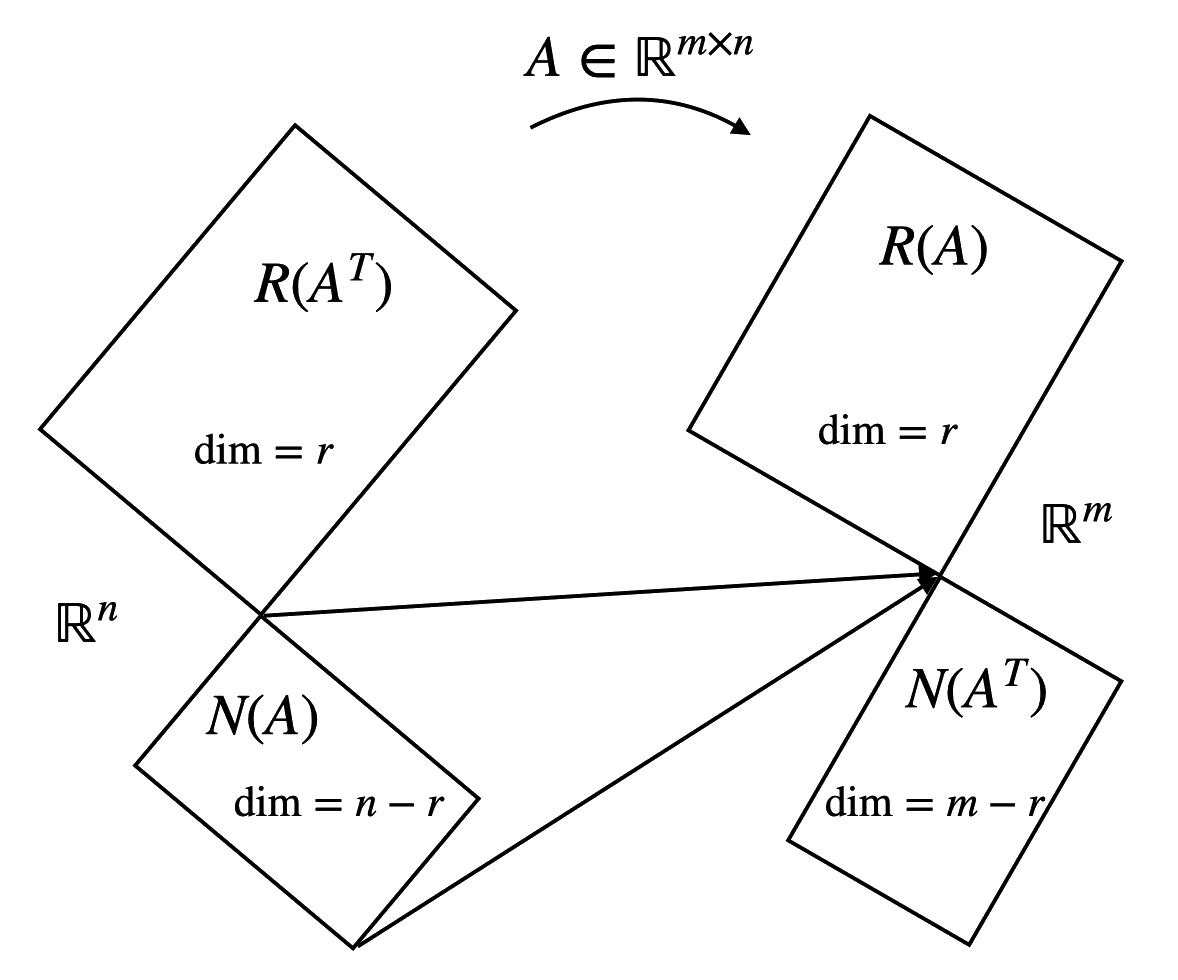
\includegraphics[width=0.55\linewidth]{figs/space.png}
\end{figure}
\end{remark}


\subsection{线性映射及其矩阵表示}

表示是什么？表示究其本质来说是一种映射，它把我们不熟悉或抽象的事物映射为我们熟知或具体的事物。例如：抽象的线性空间在一个基下可表示为实或复的列向量空间。同样地，线性空间之间的线性映射都可以表示为矩阵，这正是矩阵的代数本质所在。

\begin{definition}[线性映射]
设 $X$ 和 $Y$ 是数域 $\mathbb F$ 上的两个线性空间，$T:X\to Y$ 是从 $X$ 到 $Y$ 的一个映射，若对任意 $x,y\in X,\,k\in \mathbb F$，都有：
\begin{itemize}
    \item $T(x+y)=T(x)+T(y)$
    \item $T(kx)=kT(x)$
\end{itemize}
则称 $T$ 为 $X$ 到 $Y$ 的线性映射。
\end{definition}

\begin{definition}[线性映射的矩阵表示]
\label{def:matrixrepr}
设有 $m$ 维线性空间 $W$ 和 $n$ 维线性空间 $V$，$X=(x_1,\ldots,x_m)$，$Y=(y_1,\ldots,y_n)$ 分别是 $W,V$ 的基。$X$ 被 $T$ 映射到 $V$ 中后可以由 $Y$ 线性表示，即：
\[
\begin{cases}
Tx_1=a_{11}y_1+\cdots+a_{n1}y_n\\
\quad\vdots\\
Tx_m=a_{1m}y_1+\cdots+a_{nm}y_n\\
\end{cases}
\]
写作矩阵形式为：
\[
    TX=Y
    \underbrace{\begin{bmatrix}
    a_{11}&\cdots&a_{1m}\\
    \vdots&\ddots&\vdots\\
    a_{n1}&\cdots&a_{nm}\\
    \end{bmatrix}}_A
\]
称 $A\in\mathbb F^{n\times m}$ 为 $T$ 在基 $X,Y$ 下的矩阵表示。
\end{definition}

\begin{theorem}[向量在不同基下的坐标表示的关系]
设向量 $x\in W$ 在 $X$ 下的坐标表示为 $\xi$，$Tx\in V$ 在 $Y$ 下的坐标表示为 $\eta$，$T$ 在 $X,Y$ 下的矩阵表示为 $A$，那么有 $\eta=A\xi$. 可视化如下：
\[
\begin{array}{ccccccc}
    T: & x   & \mapsto & y    & = & T & x   \\
    \downarrow & \downarrow & & \downarrow & & \downarrow & \downarrow \\
    A: & \xi & \mapsto & \eta & = & A & \xi
\end{array}
\]
\end{theorem}
\begin{proof}
$Tx=T(X\xi)=(TX)\xi=(YA)\xi=Y(A\xi)=Y\eta\implies \eta=A\xi$
\end{proof}

从定义 \ref{def:matrixrepr} 可以看见，\textbf{线性映射的矩阵表示依赖于基的选取}，即 $A=\sigma(T;X,Y)$. 既然如此，一个自然的问题就是，同一个线性映射在不同基下的矩阵表示有什么关系呢？

\begin{theorem}[同一个线性映射在不同基下的矩阵表示的关系]
设有 $m$ 维线性空间 $W$ 和 $n$ 维线性空间 $V$，$X,X'$、$Y,Y'$ 分别是 $W,V$ 的两个基，且 $X'=XC,\,Y'=YD$，其中 $C,D$ 为过渡矩阵（因而可逆）。设线性映射 $T$ 在 $X,Y$ 下的矩阵表示为 $A$，在 $X',Y'$ 下的矩阵表示为 $A'$，那么有 $A'=D^{-1}AC$.
\end{theorem}
\begin{proof}
$TX'=T(XC)=(TX)C=(YA)C=Y'D^{-1}AC=Y'A'\implies A'=D^{-1}AC$
\end{proof}

\begin{definition}[线性映射的复合]
设有线性映射 $S:W\to V$ 和 $T: V\to U$，定义它们的复合为：
\[
    T\circ S:W\to U,\quad x\mapsto(T\circ S)(x)=T(S(x))
\]
容易证明，线性映射的复合仍为线性映射。
\end{definition}

\begin{theorem}[复合线性映射的矩阵表示]
设线性空间 $W,V,U$ 中各有基 $X,Y,Z$，在这些基下 $S,T$ 的矩阵表示分别为：$A=\sigma(S;X,Y)$，$B=\sigma(T;Y,Z)$，则复合映射 $T\circ S$ 的矩阵表示为 $BA$.
\end{theorem}
\begin{proof}
$(T\circ S)(X)=T(S(X))=T(YA)=(TY)A=(ZB)A=Z(BA)$
\end{proof}

\begin{com}
可以看见 $BA$ 只与 $X,Z$ 有关，与 $Y$ 无关，即 $BA=\sigma(T\circ S;X,Z)$. 事实上，我们可以选取 $V$ 的另一组基证明这一点：设 $Y'$ 也是 $V$ 的基且 $Y=Y'C$，那么：
\begin{align*}
    &SX=YA=(Y'C)A=Y'(CA)=Y'A'\implies CA=A'\\
    &TY=T(Y'C)=(TY')C=(ZB')C=Z(B'C)=ZB\implies B'C=B
\end{align*}
因此 $BA=(B'C)A=B'(CA)=B'A'$.
\end{com}

\begin{theorem}
设$T$为线性空间$W$到线性空间$V$的线性映射，则 $W$ 内的线性子空间$W_1$在$V$中的象$V_1$为$V$的线性子空间；反之，$V$ 中的线性子空间 $V_1$ 的逆象 $T^{-1}(V_1)=\{x\mid \exists y\in V_1,\,y=Tx\}$ 也是 $W$ 中的子空间。
\end{theorem}
\begin{proof}
利用子空间的定义易证（验证是否满足两条要求即可）。
\end{proof}

\begin{theorem}
设$T$为线性空间$W$到线性空间$V$的线性映射，$W_1,W_2$为$W$内的子空间，则：
\begin{itemize}
    \item $T(W_1+W_2)=T(W_1)+T(W_2)$
    \item $T(W_1\cap W_2)\subset T(W_1)\cap T(W_2)$
\end{itemize}
\end{theorem}
\begin{proof}
先证第一条。任取 $x\in T(W_1+W_2)$，则存在 $y\in W_1+W_2$ 使得 $x=Ty$，即存在 $y_1\in W_1,\,y_2\in W_2$ 使得 $x=T(y_1+y_2)=Ty_1+Ty_2$，故 $x\in T(W_1)+T(W_2)$，因此 $T(W_1+W_2)\subset T(W_1)+T(W_2)$；另一方面，任取 $x\in T(W_1)+T(W_2)$，则存在 $x_1\in T(W_1),\,x_2\in T(W_2)$ 使得 $x=x_1+x_2$，即存在 $y_1\in W_1,\,y_2\in W_2$ 使得 $x=Ty_1+Ty_2=T(y_1+y_2)$. 由于 $y_1+y_2\in W_1+W_2$，这说明 $x\in T(W_1+W_2)$，因此 $T(W_1)+T(W_2)\subset T(W_1+W_2)$. 综上，$T(W_1+W_2)=T(W_1)+T(W_2)$.

再证第二条。任取 $x\in T(W_1\cap W_2)$，则存在 $y\in W_1\cap W_2$ 使得 $x=Ty$. 由于 $y\in W_1$，故 $x=Ty\in T(W_1)$. 同理 $x\in T(W_2)$，故 $x\in T(W_1)\cap T(W_2)$.
\end{proof}

\begin{definition}[线性映射的值域，核空间与秩]
设有线性映射 $T:W\to V$，与矩阵类似的，定义：
\begin{itemize}
    \item 值域/列空间：$R(T)=\{y\in V\mid y=Tx,\forall x\in W\}$
    \item 核空间/零空间：$N(T)=\{x\mid Tx=0,x\in W\}$
    \item 秩：$\text{rank}(T)=\dim(R(T))$
\end{itemize}
\end{definition}

\begin{com}
容易知道，给定一个基后，线性映射的值域、核空间与其矩阵表示的值域、核空间有对应关系，且秩相同。
\end{com}

\begin{theorem}[线性映射的维数公式]
设有线性映射 $T:W\to V$，则：
\[
    \dim(R(T))+\dim(N(T))=\dim(W)
\]
\end{theorem}
\begin{proof}
可以用基扩充的方式来证明，与矩阵的维数公式类似，此处略去。
\end{proof}

\begin{theorem}[线性映射全体构成线性空间]
设 $W,V$ 为数域 $\mathbb F$ 上的线性空间，$T_1,T_2: W\to V$ 为 $W$ 到 $V$ 的线性映射，对任意 $x\in W,\,k\in\mathbb F$，定义加法和数乘如下：
\begin{itemize}
    \item 加法：$(T_1+T_2)(x)=T_1(x)+T_2(x)$
    \item 数乘：$(kT_1)(x)=k(T_1(x))$
\end{itemize}
则 $W$ 到 $V$ 的线性映射全体在上述加法和数乘下构成一个线性空间。
\end{theorem}
\begin{proof}
验证线性空间的八条要求即可。
\end{proof}

\begin{theorem}
设 $W,V$ 为数域 $\mathbb F$ 上的线性空间，$T_1,T_2: W\to V$ 为 $W$ 到 $V$ 的线性映射，任取 $W,V$ 中的基 $X,Y$，设 $T_1$ 在基 $X,Y$ 下的矩阵表示为 $A$，$T_2$ 在基 $X,Y$ 下的矩阵表示为 $B$，则有：
\begin{itemize}
    \item 线性映射 $T_1+T_2$ 的矩阵表示为 $A+B$；
    \item 线性映射 $kT_1$ 的矩阵表示为 $kA$，其中 $k\in\mathbb F$.
\end{itemize}
\end{theorem}
\begin{proof}\ 
\begin{gather*}
    (T_1+T_2)X=T_1X+T_2X=YA+YB=Y(A+B)\\
    (kT_1)X=k(T_1X)=k(YA)=Y(kA)
\end{gather*}
\end{proof}

根据上文的讨论，我们在研究线性映射时可以去研究其矩阵表示；反过来，研究矩阵时可以将其视作某线性映射的表示，或者更直接的，视作 $\mathbb F^n$ 空间到 $\mathbb F^m$ 空间的线性映射。换句话说，\textbf{我们可以借助矩阵来研究线性映射的性质，或借助线性映射来研究矩阵的性质}，这样的视角常常会带来方便，在下文中将反复用到。例如下面的定理。

\begin{theorem}
设 $A\in\mathbb F^{m\times n}$，$B\in\mathbb F^{n\times p}$，则：
\begin{gather*}
    \dim(N(AB))=\dim(N(B))+\dim(N(A)\cap R(B))\\
    \dim(R(AB))=\dim(R(B))-\dim(N(A)\cap R(B))
\end{gather*}
\end{theorem}

\begin{remark}
只从矩阵的观点看待这两个公式会难以直观理解，但若将矩阵 $A,B$ 看作线性映射，那么这两条定理可以按下图理解：
\begin{figure}[H]
    \centering
    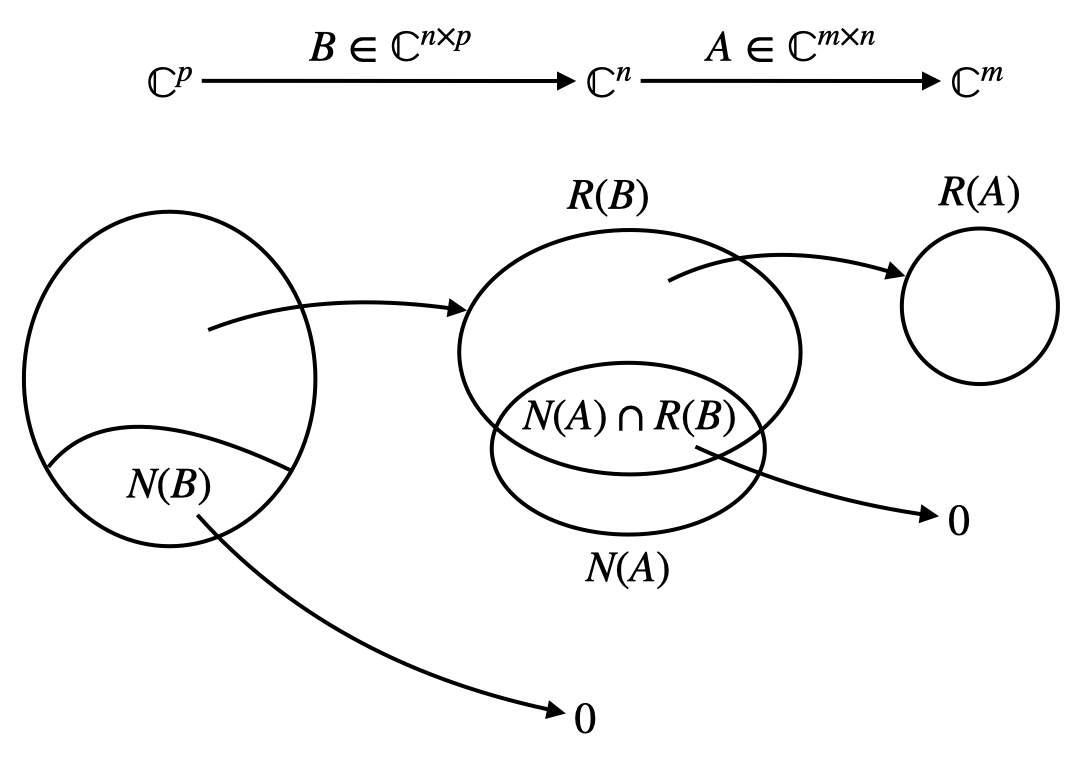
\includegraphics[width=0.6\linewidth]{figs/mapping.png}
\end{figure}
\begin{itemize}
    \item $N(AB)$ 包含被 $B$ 映射到了 $0$ 的部分和没被 $B$ 映射到 $0$、但被 $A$ 映射到 $0$ 的部分。
    \item $R(AB)$ 是没有被 $B$ 映射到 $0$ 的部分中，也没有被 $A$ 映射到 $0$ 的部分。
\end{itemize}
\end{remark}

\begin{proof}
首先证明第一个式子，依旧采用基扩充的思路。存在一组线性无关的 $x_1,\ldots,x_r\in\mathbb C^p$ 使得 $(Bx_1,\ldots,Bx_r)$ 为 $N(A)\cap R(B)$ 的一个基，再取 $N(B)$ 的一个基 $(y_1,\ldots,y_s)$，则只需要证明 $(x_1,\ldots,x_r,y_1,\ldots,y_s)$ 构成 $N(AB)$ 的一个基即可。

首先证明线性无关。由于 $(x_1,\ldots,x_r)$ 线性无关，$(y_1,\ldots,y_s)$ 线性无关，因此只需要证明 $y_j\ (j=1,\ldots,s)$ 与 $(x_1,\ldots,x_r)$ 线性无关即可。这是容易的，因为 $y_j\in N(B),\,x_i\in R(B)$，而 $N(B)\cap R(B)=\{0\}$.

其次，任取 $z\in N(AB)$，那么 $ABz=0$.  当 $Bz=0$ 时，$z\in N(B)$，可以被 $(y_1,\ldots,y_s)$ 线性表示；当 $Bz\neq 0$ 时，$Bz\in N(A)\cap R(B)$，因此 $Bz$ 可以被 $(Bx_1,\ldots,Bx_r)$ 线性表示，即：
\[
    Bz=\sum_{i=1}^r a_i Bx_i\implies B\left(z-\sum_{i=1}^ra_ix_i\right)=0
\]
但由于 $z,x_i\notin N(B)$，所以只能是括号内为零，即 $z$ 可以被 $(x_1,\ldots,x_r)$ 线性表示。

对于第二个式子，可以类似地采用基扩充的思路证明，这里选择另一种方法。利用上一条定理的结论，结合：
\[
    \dim(R(AB))+\dim(N(AB))=\dim(R(B))+\dim(N(B))=p
\]
即可推出结论。
\end{proof}

\begin{corollary}
设 $A\in\mathbb F^{m\times n}$，$B\in\mathbb F^{n\times p}$，$C\in\mathbb F^{p\times q}$，则：
\begin{gather*}
    \text{rank}(A)+\text{rank}(B)-n\leq \text{rank}(AB)\\
    \dim(R(AB))+\dim(R(BC))-\dim(R(B))\leq \dim(R(ABC))
\end{gather*}
\end{corollary}
\begin{proof}
1) 由于：
\[
    \dim(R(B))-\dim(R(AB))=\dim(N(A)\cap R(B))\leq\dim(N(A))=n-\dim(R(A))
\]
等号成立当且仅当 $N(A)\subset R(B)$. 所以：
\[
    \dim(R(A))+\dim(R(B))-n\leq\dim(R(AB))
\]
即 $\text{rank}(A)+\text{rank}(B)-n\leq \text{rank}(AB)$.

2) 类似地，由于：
\begin{align*}
    \dim(R(BC))-\dim(R(ABC))&=\dim(N(A)\cap R(BC))\\
    &\leq \dim(N(A)\cap R(B))=\dim(R(B))-\dim(R(AB))
\end{align*}
所以：
\[
    \dim(R(AB))+\dim(R(BC))-\dim(R(B))\leq \dim(R(ABC))
\]
等号成立的条件为 $N(A)\cap R(BC)=N(A)\cap R(B)$.
\end{proof}

\begin{definition}[线性变换]
线性变换是从一个线性空间映射到它本身的线性映射，即 $T:W\to W$.
\end{definition}

\begin{definition}[线性变换的矩阵表示]
由于线性变换只涉及一个空间，所以当我们讨论线性映射的矩阵表示时，只需选择一个基 $X$，于是有 $TX=XA$，称方阵 $A$ 是线性变换 $T$ 的矩阵表示。
\end{definition}
\begin{com}
当然，也可以选择两个不同的基 $X,Y$，这时相当于把线性变换依旧视作线性映射。本课程以后提到线性变换时都只选择一个基。
\end{com}

与线性映射在不同基下有不同的矩阵表示类似，线性变换在不同基下也有着不同的矩阵表示，这引出了相似矩阵的定义。

\begin{theorem}[线性变换在不同基下的矩阵表示]
\label{thm:sim-trans}
设线性变换 $T$ 在基 $X$ 下的矩阵表示为 $A$，在基 $X'$ 下的矩阵表示为 $A'$，且两个基之间的关系为 $X'=XC$，那么 $A'=C^{-1}AC$.
\end{theorem}
\begin{proof}
$TX'=TXC=XAC=X'C^{-1}AC=X'A'\implies A'=C^{-1}AC$
\end{proof}

\begin{definition}[相似矩阵]
设 $A,A'$ 为 $n$ 阶矩阵，若存在 $n$ 阶可逆矩阵 $C$ 使得 $A'=C^{-1}AC$，则称 $A$ 与 $A'$ 是相似的。
\end{definition}

\begin{property}
矩阵相似关系为等价关系，即满足：
\begin{itemize}
    \item 自反性：$A$ 和 $A$ 相似；
    \item 对称性：若 $A$ 和 $B$ 相似，则 $B$ 和 $A$ 相似；
    \item 传递性：若 $A$ 和 $B$ 相似，$B$ 和 $C$ 相似，则 $A$ 和 $C$ 相似。
\end{itemize}
\end{property}

\begin{remark}
可以看见，相似矩阵本质上是同一个线性变换在不同基下的表示。因此，\textbf{相似等价意义下矩阵具有的性质本质上是对应线性变换的性质}。例如，我们即将看见相似矩阵的行列式相同，本质这是因为行列式对应着线性变换对原空间的单位超立方体变换后的体积。
\end{remark}

\begin{definition}[线性变换的多项式]
记 $T^2$ 表示复合变换 $T\circ T$，记 $T^k=T^{k-1}\circ T$. 进一步地，设 $f(\cdot)$ 是一个多项式：$f(x)=a_0x^m+a_1x^{m-1}+\cdots+a_{m-1}x+a_m$，则记线性变换的多项式为 $f(T)=a_0T^m+a_1T^{m-1}+\cdots+a_{m-1}T+a_mI$.
\end{definition}

\begin{theorem}[线性变换的多项式的矩阵表示]
若 $T$ 的矩阵表示为 $A$，那么 $T^k$ 的矩阵表示为 $A^k$；进一步地，多项式 $f(T)$ 的矩阵表示为 $f(A)$.
\end{theorem}

\begin{com}
上面定义了线性变换的多项式，自然地，我们思考能否定义线性变换的一般函数，例如 $\exp(T)$ 或 $\sin(T)$？不过，这个问题需要 Hamilton-Cayley 定理（定理 \ref{thm:Hamilton-Cayley}）和第三章的相关知识，我们将在 \ref{sec:3-matrix-function} 节中给出答案。
\end{com}


\subsection{特征值与特征向量，对角化}

由于线性变换在不同基下的矩阵表示不相同，那么一个很自然的问题就是，怎样选择特殊的基使得给定线性变换在这个基下的表示矩阵尽可能简单（有尽可能多的 0）？为了解决这个问题，我们首先要介绍有关特征值与特征向量的基础知识。

\begin{definition}[线性变换的特征值与特征向量]
设 $T$ 是一个线性变换，若存在非零向量 $x$ 和数 $\lambda$ 满足 $Tx=\lambda x$，则称 $\lambda$ 为 $T$ 的特征值，$x$ 为属于 $\lambda$ 的特征向量。
\end{definition}

\begin{definition}[矩阵的特征值与特征向量]
设 $A$ 为 $n$ 阶矩阵，若存在非零向量 $x$ 和数 $\lambda$ 满足 $Ax=\lambda x$，则称 $\lambda$ 为矩阵 $A$ 的特征值，$x$ 为属于 $\lambda$ 的特征向量。
\end{definition}

\begin{theorem}[线性变换的特征值和特征向量与矩阵的特征值和特征向量]
\label{thm:eigen-transform-matrix}
设 $X$ 为线性空间中的一个基，线性变换 $T$ 在该基下的矩阵表示为 $A$. 若 $\lambda$ 为 $T$ 的一个特征值，对应特征向量 $x$ 在基 $X$ 下的坐标表示为 $\xi$，则 $\lambda$ 是 $A$ 的特征值，$\xi$ 是对应的特征向量。
\end{theorem}
\begin{proof}
由题意有 $x=X\xi,\,TX=XA,\,Tx=\lambda x$，因此：
\[
    \begin{cases}
    Tx=T(X\xi)=(TX)\xi=XA\xi\\
    Tx=\lambda x=\lambda X\xi=X(\lambda\xi)
    \end{cases}\implies A\xi=\lambda\xi
\]
即 $\lambda$ 是 $A$ 的特征值，$\xi$ 是对应的特征向量。
\end{proof}

上述定理说明，线性变换的特征值和其矩阵表示的特征值是一样的，而特征向量的关系就是在选取的那个基下的坐标关系。因此对于特征值和特征向量，我们有两个刻画的角度——从几何的角度，特征向量是经过线性变换后方向不变的向量，特征值为其长度伸缩量；从代数的角度，特征值与特征向量是一个矩阵方程的解。视角的不同会给我们带来不同的定义和结论，但本质的相同说明这些结论之间有着密切的联系。

% \begin{theorem}
% $n$ 阶矩阵 $A$ 奇异当且仅当 $0$ 是 $A$ 的特征值。
% \end{theorem}
% \begin{proof}
% $n$ 阶矩阵 $A$ 奇异 $\iff$ 存在 $x\neq0$ 使得 $Ax=0$ $\iff$ 存在 $x\neq0$ 使得 $Ax=0\cdot x$ $\iff$ $0$ 是 $A$ 的特征值。
% \end{proof}

首先从代数的角度看，设 $\lambda,\,x\neq0$ 是矩阵 $A$ 的特征值和对应特征向量，则有 $Ax=\lambda x$，即 $(\lambda I-A)x=0$. 由于 $x\neq 0$，因此该方程有解当且仅当 $\lambda I-A$ 奇异，即 $\det(\lambda I-A)=0$. 据此我们给出特征多项式、特征方程与代数重数的定义。

\begin{definition}[特征多项式，特征方程]
设 $A$ 为一个 $n$ 阶矩阵，称多项式 $\varphi(\lambda)=\det(\lambda I-A)$ 为矩阵 $A$ 的特征多项式，方程 $\det(\lambda I-A)=0$ 为矩阵 $A$ 的特征方程。
显然，特征多项式 $\varphi(\lambda)$ 的零点（即特征方程的根）就是矩阵 $A$ 的特征值。
\end{definition}

进一步地，根据\textbf{代数基本定理}，$n$ 阶多项式在\textbf{复数域}中必有 $n$ 个零点（可能重合），因此为了方便起见，我们定义特征值的代数重数如下。

\begin{definition}[代数重数]
设 $A$ 为一个 $n$ 阶矩阵，$\lambda_0$ 为其一个特征值，称 $\lambda_0$ 作为特征多项式 $\varphi(\lambda)$ 的零点的重数为它的代数重数。
\end{definition}

由于特征多项式是一个 $n$ 阶多项式，我们现在就可以直接断言：\textbf{任意 $n$ 阶矩阵在复数域中恰有 $n$ 个特征值（相同特征值按其代数重数计数）}。设这 $n$ 个特征值为 $\lambda_1,\lambda_2,\ldots,\lambda_n$（重复特征值重复写出），那么特征多项式也可以写作 $\varphi(\lambda)=(\lambda-\lambda_1)(\lambda-\lambda_2)\cdots(\lambda-\lambda_n)$. 基于此，通过探究特征多项式根与系数的关系，我们可以得到下述常用结论。

\begin{theorem}[迹与特征值，行列式与特征值]
\ 
\begin{enumerate}
    \item 矩阵 $A$ 的迹等于 $A$ 的所有特征值之和；
    \item 矩阵 $A$ 的行列式等于 $A$ 的所有特征值之积。
\end{enumerate}
\end{theorem}
\begin{proof}
设矩阵 $A$ 的特征值为 $\lambda_1,\lambda_2,\ldots,\lambda_n$，则特征多项式可写作：
\begin{align*}
    \varphi(\lambda)&=(\lambda-\lambda_1)(\lambda-\lambda_2)\cdots(\lambda-\lambda_n)\\
    &=\lambda^n-(\lambda_1+\lambda_2+\cdots+\lambda_n)\lambda^{n-1}+\cdots+(-1)^n\lambda_1\lambda_2\cdots\lambda_n
\end{align*}
另一方面，根据定义：
\[
    \varphi(\lambda)=\det(\lambda I-A)=
    \begin{vmatrix}
    \lambda-a_{11}&-a_{12}&\cdots&-a_{1n}\\
    -a_{21}&\lambda-a_{22}&\cdots&-a_{2n}\\
    \vdots&\vdots&\ddots&\vdots\\
    -a_{n1}&-a_{n2}&\cdots&\lambda-a_{nn}
    \end{vmatrix}
\]
将行列式按第一行展开，可以发现含有 $\lambda^n$ 和 $\lambda^{n-1}$ 的只有一项：
\[
    (\lambda-a_{11})(\lambda-a_{22})\cdots(\lambda-a_{nn})
\]
这是因为其他项最高只到 $\lambda^{n-2}$. 因此，对比二式中 $\lambda^{n-1}$ 的系数可知：
\[
    \lambda_1+\lambda_2+\cdots+\lambda_n=a_{11}+a_{22}+\cdots+a_{nn}=\text{tr}(A)
\]
即矩阵 $A$ 的迹等于 $A$ 的所有特征值之和。另外，在特征多项式中代入 $\lambda=0$，得：
\[
    \det(-A)=(-1)^n\det(A)=(-1)^n\lambda_1\lambda_2\cdots\lambda_n
\]
因此有：
\[
    \det(A)=\lambda_1\lambda_2\cdots\lambda_n
\]
即矩阵 $A$ 的行列式等于 $A$ 的所有特征值之积。
\end{proof}

\begin{theorem}
\label{thm:sim-eigen}
相似矩阵有相同的特征多项式。
\end{theorem}
\begin{proof}
设 $A$ 与 $B$ 相似，则存在可逆矩阵 $P$ 使得 $P^{-1}AP=B$，于是：
\begin{align*}
    \det(\lambda I-B)&=\det(P^{-1}(\lambda I)P-P^{-1}AP)=\det(P^{-1}(\lambda I-A)P)\\
    &=\det(P^{-1})\det(\lambda I-A)\det(P)=\det(\lambda I-A)
\end{align*}
即 $A$ 与 $B$ 的特征多项式相同。
\end{proof}

\begin{corollary}
\label{thm:sim-eigenvalue}
相似矩阵的特征值相同，进而迹相同、行列式相同。
\end{corollary}

\begin{theorem}[$AB$ 和 $BA$ 有相同的非零特征值]
\label{thm:eigen-ab-ba}
设 $A\in\mathbb C^{m\times n},B\in\mathbb C^{n\times m}$，记 $AB$ 的特征多项式为 $\varphi_{AB}(\lambda)$，$BA$ 的特征多项式为 $\varphi_{BA}(\lambda)$，则：
\[
    \lambda^n\varphi_{AB}(\lambda)=\lambda^m\varphi_{BA}(\lambda)
\]
即 $AB$ 和 $BA$ 有相同的非零特征值。
\end{theorem}
\begin{proof}
由于：
\[
    \begin{bmatrix}I_m&0\\-B&I_n\end{bmatrix}\begin{bmatrix}I_m&A\\0&\lambda I_n\end{bmatrix}\begin{bmatrix}\lambda I_m-AB&0\\B&I_n\end{bmatrix}=\begin{bmatrix}I_m&A\\0&\lambda I_n-BA\end{bmatrix}
\]
等式两边取行列式即得证。
\end{proof}
\begin{proof}[更直接的证明方法]
设 $\lambda,x$ 为 $AB$ 的特征值和特征向量，即 $ABx=\lambda x$，那么左乘 $B$ 得到：\[(BA)(Bx)=\lambda (Bx)\]
也就是说 $\lambda$ 和 $Bx$ 是 $BA$ 的特征值和特征向量。
\end{proof}

\begin{corollary}
设 $A\in\mathbb C^{m\times n},B\in\mathbb C^{n\times m}$，则 $\text{tr}(AB)=\text{tr}(BA)$，$\det(AB)=\det(BA)$.
\end{corollary}

\begin{corollary}
\label{cor:trace}
设 $A\in\mathbb C^{m\times n},B\in\mathbb C^{n\times p},C\in\mathbb C^{p\times m}$，则 $\text{tr}(ABC)=\text{tr}(BCA)=\text{tr}(CAB)$. 以此类推，对于更多矩阵相乘的情形有类似的轮换性质。
\end{corollary}

\begin{theorem}
\label{thm:anysimilar}
任意 $n$ 阶矩阵都相似于上三角矩阵。
\end{theorem}
\begin{proof}
考虑数学归纳法。设 $A$ 是一个 $n$ 阶矩阵，$x_1$ 为 $A$ 的特征值 $\lambda$ 对应的特征向量。将 $x_1$ 扩充为 $\mathbb C^n$ 的一个基 $(x_1,\ldots,x_n)$，那么 $Ax_i$ 都可以被这个基线性表示：
\[
    \begin{cases}
    Ax_1=b_{11}x_1+b_{21}x_2+\cdots+b_{n1}x_n=\lambda x_1\\
    Ax_2=b_{12}x_1+b_{22}x_2+\cdots+b_{n2}x_n\\
    \quad\vdots\\
    Ax_n=b_{1n}x_1+b_{2n}x_2+\cdots+b_{nn}x_n
    \end{cases}
\]
写作矩阵形式：
\[
    AX=XB=X\begin{bmatrix}\lambda&b_{12}&\cdots&b_{1n}\\0&b_{22}&\cdots&b_{2n}\\\vdots&\vdots&\ddots&\vdots\\0&b_{n2}&\cdots&b_{nn}\end{bmatrix}=X\begin{bmatrix}\lambda&\alpha^T\\0&B_1\end{bmatrix}
\]
根据归纳假设，可设 $B_1=QUQ^{-1}$ 且 $U$ 是上三角矩阵，那么：
\[
    AX=X\begin{bmatrix}\lambda&\alpha^T\\0&QUQ^{-1}\end{bmatrix}=X\begin{bmatrix}1&0\\0&Q\end{bmatrix}\begin{bmatrix}\lambda&\alpha^T\\0&U\end{bmatrix}\begin{bmatrix}1&0\\0&Q^{-1}\end{bmatrix}
\]
所以 $A$ 相似于上三角矩阵 $\begin{bmatrix}\lambda&\alpha^T\\0&U\end{bmatrix}$.
\end{proof}

\begin{definition}[零化多项式]
设 $A$ 是一个 $n$ 阶矩阵，若多项式 $f(\cdot)$ 使得 $f(A)=0$，则称 $f(\cdot)$ 为矩阵 $A$ 的一个零化多项式。
\end{definition}

\begin{theorem}[Hamilton-Cayley 定理]
\label{thm:Hamilton-Cayley}
设 $A$ 是一个 $n$ 阶矩阵，则 $A$ 的特征多项式是其零化多项式。
\end{theorem}

\begin{proof}
考虑数学归纳法。首先，当 $n=1$ 时，定理显然成立；其次，设定理对 $n-1$ 阶矩阵成立，下面证明对 $n$ 阶矩阵依然成立。设 $A$ 的 $n$ 个特征值为 $\lambda_1,\ldots,\lambda_n$，根据定理 \ref{thm:anysimilar} 的证明过程可知，$A$ 相似于：
\[R=\begin{bmatrix}\lambda_1&\alpha^T\\0&U\end{bmatrix}\]
即存在可逆矩阵 $P$ 使得 $A=P^{-1}RP$，其中 $U$ 为上三角矩阵。由于相似矩阵有相同的特征值，所以 $\lambda_1,\ldots,\lambda_n$ 也是 $R$ 的特征值，进而可知 $\lambda_2,\ldots,\lambda_n$ 是 $U$ 的特征值。设 $A$ 的特征多项式为 $\varphi(\lambda)=\sum_{i=0}^ma_{n-i}\lambda^i=(\lambda-\lambda_1)\cdots(\lambda-\lambda_n)$，则：
\[
    \varphi(A)=\varphi(P^{-1}RP)=\sum_{i=0}^n a_{n-i}(P^{-1}RP)^i=\sum_{i=0}^n a_{n-i}P^{-1}R^iP=P^{-1}\varphi(R)P
\]
所以要证明 $\varphi(A)=0$，只需要证明 $\varphi(R)=0$.
\begin{align*}
    \varphi(R)&=(R-\lambda_1I_n)\cdots(R-\lambda_n I_n)\\
    &=\begin{bmatrix}\lambda_1-\lambda_1&\alpha^T\\0&U-\lambda_1I_{n-1}\end{bmatrix}\cdots\begin{bmatrix}\lambda_n-\lambda_1&\alpha^T\\0&U-\lambda_nI_{n-1}\end{bmatrix}\\
    &=\begin{bmatrix}0&\alpha^T\\0&U-\lambda_1I_{n-1}\end{bmatrix}\begin{bmatrix}\prod_{j=2}^n(\lambda_j-\lambda_1)&\beta^T\\0&\prod_{j=2}^n(U-\lambda_jI_{n-1})\end{bmatrix}\\
    &=\begin{bmatrix}0&0\\0&(U-\lambda_1 I_{n-1})\prod_{j=2}^n(U-\lambda_jI_{n-1})\end{bmatrix}
\end{align*}
根据归纳假设，$\prod_{j=2}^n(U-\lambda_jI_{n-1})=0$，因此上式为 $0$.
\end{proof}

\begin{corollary}
对于 $n$ 阶矩阵 $A$，$\{A^n,A^{n-1},\ldots,A,I_n\}$ 线性相关。
\end{corollary}

\begin{corollary}
\label{cor:invpoly}
任何一个 $n$ 阶可逆矩阵 $A$ 的逆可表示为 $A$ 的次数不超过 $n-1$ 的多项式，即：
\[
    A^{-1}=g(A)=a_1A^{n-1}+a_2A^{n-2}+\cdots+a_{n-1}A+a_nI_n
\]
\end{corollary}

\begin{definition}[最小多项式]
称次数最低的首项系数为 1 的零化多项式 $m(\cdot)$ 为最小多项式。
\end{definition}

\begin{theorem}
\label{thm:minpoly}
最小多项式可以整除任意其他首项系数为 1 的零化多项式，且是唯一的。
\end{theorem}
\begin{proof}
设 $\psi(\cdot)$ 是一个首项系数为 1 的零化多项式，作多项式除法：$\psi(\lambda)=m(\lambda)p(\lambda)+r(\lambda)$，其中 $r(\lambda)$ 的次数小于 $m(\lambda)$ 的次数。由于 $\psi(A)=m(A)=0$，故 $r(A)=0$，但由于 $m(\lambda)$ 是次数最小的零化多项式，所以只能是 $r(\lambda)=0$. 因此 $m(\lambda)\mid\psi(\lambda)$.
\end{proof}

\begin{theorem}
矩阵 $A$ 的最小多项式 $m(\lambda)$ 和特征多项式 $\varphi(\lambda)$ 零点相同（重数可以不同）。换句话说，$m(\lambda)$ 的零点就是特征值，只是与 $\varphi(\lambda)$ 的次数不同。
\end{theorem}
\begin{proof}
根据定理 \ref{thm:minpoly}，$\varphi(\lambda)=m(\lambda)p(\lambda)$，所以 $m(\lambda)=0\implies \varphi(\lambda)=0$. 因此现在只需证明 $\varphi(\lambda)=0\implies m(\lambda)=0$.
设 $\varphi(\lambda_0)=0$，$A x_0=\lambda_0 x_0$，则 $m(A) x_0=m(\lambda_0) x_0=0$，由于 $x_0\neq 0$，所以 $m(\lambda_0)=0$.
\end{proof}

\begin{com}
如果矩阵 $A$ 的最小多项式次数为 $m$，那么 $\{A^{m-1},\ldots,A,I_n\}$ 是一个极大线性无关组。
\end{com}

下面我们从几何的角度讨论特征值与特征向量。事实上，在这个角度下前文的一些结论将变得非常显然。例如，由于线性变换的特征值与其矩阵表示的特征值相同，而不同矩阵表示之间是相似的关系，因此前文推论 \ref{thm:sim-eigenvalue} 所述的“相似矩阵有相同的特征值”就是不言自明的。

类似地，考虑到线性变换与其矩阵表示之间的联系，前文许多对矩阵叙述的定义和定理都可以对线性变换重新叙述一遍，这里不再赘述。特别地，定理 \ref{thm:anysimilar} 说明对任意线性变换，都存在一个基使之在该基下的矩阵表示是上三角矩阵。这初步回答了本节开头的问题，但上三角矩阵仍然太多，不够简单，我们还需要继续努力。

设 $\lambda,\,x\neq0$ 是线性变换 $T$ 的特征值和对应特征向量，则有 $Tx=\lambda x$，即 $(\lambda I-T)x=0$，其中 $I$ 表示恒等变换。这说明 $x\in N(\lambda I-T)$，据此我们给出特征子空间与几何重数的定义。

\begin{definition}[特征子空间]
设 $\lambda_0$ 为线性变换 $T$ 的特征值，则称 $\lambda_0I-T$ 的核空间为 $T$ 属于 $\lambda_0$ 的特征子空间，记作 $E(\lambda_0,T)$，即：
\[
    E(\lambda_0,T)=N(\lambda_0I-T)=\{x\mid(\lambda_0 I-T)x=0\}
\]
显然，$E(\lambda_0,T)$ 中的所有向量就是 $T$ 属于 $\lambda_0$ 的特征向量。
\end{definition}

\begin{definition}[几何重数]
设 $T$ 为线性变换，$\lambda_0$ 为其特征值，称 $\dim E(\lambda_0,T)$ 为 $\lambda_0$ 的几何重数。
\end{definition}

\begin{theorem}[代数重数 $\geq$ 几何重数]
设 $T$ 为线性空间 $V$ 上的线性变换，$\lambda_0$ 为 $T$ 的一个特征值，则其代数重数大于等于几何重数。
\end{theorem}
\begin{proof}
设几何重数 $\dim E(\lambda_0,T)=q$，取 $E(\lambda_0,T)$ 的基 $x_1,\ldots,x_q$，将其扩充为 $V$ 的基 $x_1,\ldots,x_q,\ldots,x_n$. 由于对 $i=1,2,\ldots,q$，有 $Tx_i=\lambda_0x_i$，因此 $T$ 在基 $x_1,\ldots,x_q,\ldots,x_n$ 下的矩阵表示为：
\[
    A=\left[\begin{array}{ccc:ccc}
    \lambda_0 & \cdots & 0         & &        & \\
    \vdots    & \ddots & \vdots    & & A_{12} & \\
    0         & \cdots & \lambda_0 & &        & \\ \hdashline
              &        &           & &        & \\
              & O      &           & & A_{22} & \\
              &        &           & &        & \\
    \end{array}\right]
\]
于是特征多项式为：
\[
    \varphi(\lambda)=\det(\lambda I-A)=(\lambda-\lambda_0)^q\det(\lambda I_{n-q}-A_{22})
\]
故代数重数至少为 $q$.
\end{proof}

\begin{theorem}[特征向量的线性无关性]
\label{thm:eigenind}
设 $\lambda_1,\ldots,\lambda_s$ 为线性变换 $T$ 的\textbf{互不相同}的特征值，$x_1,\ldots,x_s$ 是分别属于这些特征值的特征向量，那么 $x_1,\ldots,x_s$ 线性无关。
\end{theorem}
\begin{proof}
考虑数学归纳法。首先，单个特征向量 $x_1$ 线性无关；其次，假设 $x_1,\ldots,x_{s-1}$ 线性无关，设 $\sum_{i=1}^s k_ix_i=0$，则：
\[
    T\left(\sum_{i=1}^sk_ix_i\right)=\sum_{i=1}^sk_iTx_i=\sum_{i=1}^sk_i\lambda_ix_i=0
\]
根据上面两个式子消去 $x_s$，得：
\[
    \sum_{i=1}^{s-1}k_i(\lambda_i-\lambda_s)x_i=0
\]
根据归纳假设，有 $k_i(\lambda_i-\lambda_s)=0,\,i=1\ldots,s-1$；又特征值互不相同，故 $k_i=0,\,i=1,\ldots,s-1$. 进而 $k_s=0$.
\end{proof}

\begin{theorem}[特征向量的线性无关性]
设 $\lambda_1,\ldots,\lambda_k$ 为线性变换 $T$ 的\textbf{互不相同}的特征值，$x_{i1},\ldots,x_{ir_i}$ 是属于 $\lambda_i$ 的线性无关特征向量，那么 $x_{11},\ldots,x_{1r_1},\ldots,x_{k1},\ldots,x_{kr_k}$ 线性无关。
\end{theorem}
\begin{proof}
设 $\sum_{i=1}^k\sum_{j=1}^{r_i}k_{ij}x_{ij}=0$，记 $x_i=\sum_{j=1}^{r_i}k_{ij}x_{ij}$，则：
\[
    Tx_i=T\left(\sum_{j=1}^{r_i}k_{ij}x_{ij}\right)=\sum_{j=1}^{r_i}k_{ij}Tx_{ij}=\sum_{j=1}^{r_i}k_{ij}\lambda_ix_{ij}=\lambda_ix_i
\]
假设 $x_i\neq0$，则 $x_i$ 是 $A$ 属于 $\lambda_i$ 的特征向量，又由于 $\sum_{i=1}^kx_i=0$，根据定理 \ref{thm:eigenind} 知 $x_i=0$，矛盾，因此只能有 $x_i=0$. 由线性无关性可知，所有的 $k_{ij}=0$.
\end{proof}

\begin{definition}[不变子空间]
若线性空间 $V$ 的线性子空间 $V_1$ 对线性变换 $T$ 保持不变，即：$\forall x\in V_1$，有 $Tx\in V_1$，则称 $V_1$ 是 $T$ 的不变子空间。这时 $T$ 可以看作 $V_1$ 上的线性变换，称为 $T$ 在 $V_1$ 上的限制 $T\vert V_1$.  但值得注意的是，$T$ 和 $T\vert V_1$ 是不同的线性变换（它们的输入维度都不同）。
\end{definition}
\begin{figure}[H]
    \centering
    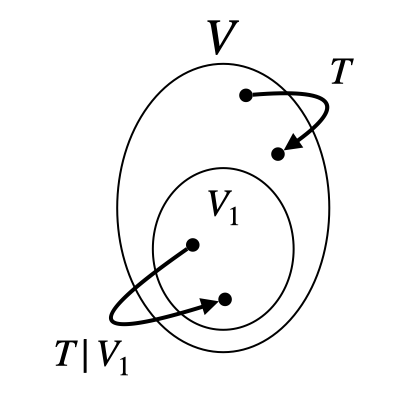
\includegraphics[width=0.2\linewidth]{figs/TV1.png}
\end{figure}

\begin{theorem}
不变子空间的和与交也是不变子空间。
\end{theorem}
\begin{proof}
设 $V_1,V_2$ 都是 $T$ 的不变子空间，则对于 $z\in V_1+V_2$，存在 $x\in V_1,\,y\in V_2$ 使得 $z=x+y$，并且 $Tx\in V_1,\,Ty\in V_2$，于是 $Tz=T(x+y)=Tx+Ty\in V_1+V_2$. 另外，对于 $z\in V_1\cap V_2$，由于 $Tz\in V_1,\,Tz\in V_2$，故 $Tz\in V_1\cap V_2$.
\end{proof}

\begin{theorem}
线性变换 $T$ 的值域 $R(T)$ 和核 $N(T)$ 都是 $T$ 的不变子空间。
\end{theorem}
\begin{proof}
对 $\forall x\in R(T)$，$Tx\in R(T)$，故 $R(T)$ 是 $T$ 的不变子空间；对于 $\forall x\in N(T)$，$Tx=0\in N(T)$，故 $N(T)$ 是 $T$ 的不变子空间。
\end{proof}

\begin{theorem}
设 $x$ 是线性变换 $T$ 的特征向量，则 $L(x)$ 是 $T$ 的一维不变子空间。
\end{theorem}
\begin{proof}
根据特征值和特征向量的定义易证。
\end{proof}

\begin{theorem}
设 $f(t)$ 为一多项式，则 $T$ 的不变子空间也是 $f(T)$ 的不变子空间。
\end{theorem}
\begin{proof}
设 $V_1$ 是 $T$ 的不变子空间，即 $\forall x\in V_1$，有 $Tx\in V_1$.  那么 $T^2x=T(Tx)\in V_1$，以此类推有 $f(T)(x)\in V_1$，即 $V_1$ 也是 $f(T)$ 的不变子空间。
\end{proof}

\begin{corollary}
若 $T$ 为可逆变换，则 $T$ 的不变子空间也是 $T^{-1}$ 的不变子空间。
\end{corollary}
\begin{proof}
根据推论 \ref{cor:invpoly}，$T^{-1}$ 可写作 $T$ 的多项式，故可得结论。
\end{proof}

\begin{corollary}
特征子空间为不变子空间。
\end{corollary}
\begin{proof}
注意到 $\lambda I-T$ 是 $T$ 的多项式，故 $E(\lambda,T)=N(\lambda I-T)$ 为 $T$ 的不变子空间。
\end{proof}

基于不变子空间的概念，下面引入分块对角化与对角化。

\begin{theorem}[分块对角化]
\label{thm:blockdiag}
设 $T$ 是 $n$ 维线性空间 $V$ 上的线性变换，假若 $V$ 可以分解为 $s$ 个 $T$ 的不变子空间的直和：
\[
    V=V_1\oplus\cdots\oplus V_s
\]
则 $T$ 在 $V$ 的某个基下的矩阵表示为分块对角矩阵：
\[
    A=\begin{bmatrix}A_1&&\\&\ddots&\\&&A_s\end{bmatrix}
\]
反之，若 $T$ 在基 $X=(X_1,\ldots,X_s)$ 下的矩阵表示为分块对角矩阵，则 $V$ 可分解为 $s$ 个不变子空间的直和。
\begin{figure}[H]
    \centering
    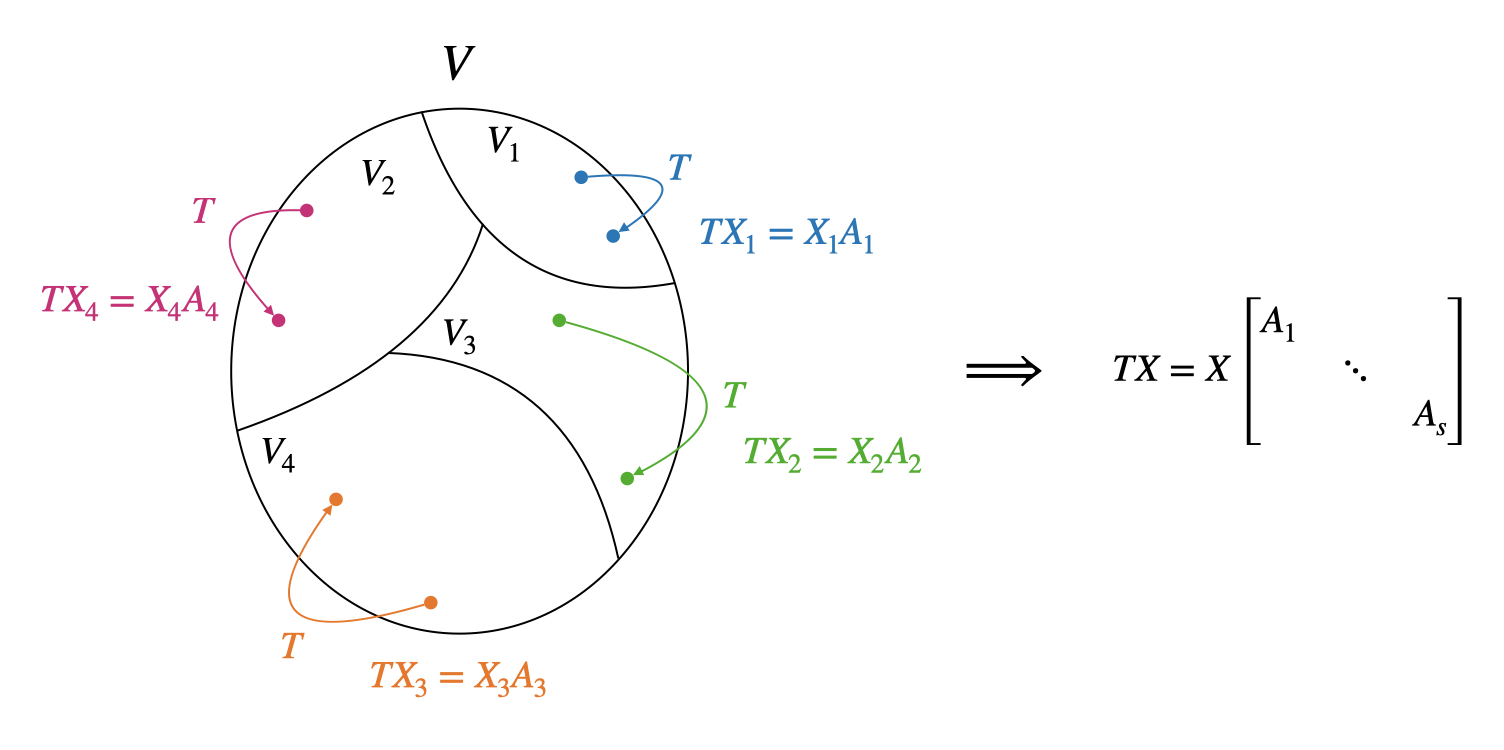
\includegraphics[width=0.75\linewidth]{figs/subspaces.png}
\end{figure}
\end{theorem}
\begin{proof}
设 $V$ 可以分解为 $s$ 个不变子空间的直和，在每个不变子空间 $V_i$ 中选取一个基 $X_i=(x_{i1},\ldots,x_{in_i}),\,(i=1,\ldots,s)$，将它们合并构成 $V$ 的基 $X=(X_1,\ldots,X_s)$，则显然 $T$ 在这个基下的矩阵表示为一个分块对角矩阵。反之，若 $T$ 在基 $X=(X_1,\ldots,X_s)$ 下的矩阵表示为分块对角矩阵，那么根据定义容易知道 $X_i$ 张成的子空间 $V_i$ 是 $T$ 的不变子空间，且 $V$ 是它们的直和。
\end{proof}

\begin{definition}[可对角化]
若 $n$ 维线性空间 $V$ 上的线性变换 $T$ 在 $V$ 的某个基下的表示矩阵为对角阵，则称 $T$ 是可对角化的。
\end{definition}

\begin{theorem}[可对角化的充要条件]
设 $T$ 为 $n$ 维线性空间 $V$ 上的线性变换，则 $T$ 可对角化的充要条件是存在一组特征向量构成的基，即 $T$ 有 $n$ 个线性无关的特征向量。
\end{theorem}
\begin{proof}
充分性：由于每个特征向量张成的一维子空间都是一个一维不变子空间，因此当 $T$ 有 $n$ 个线性无关的特征向量时（这些特征向量构成了一个基），$V$ 就可以写作这些特征向量分别张成的一维不变子空间的直和。于是根据定理 \ref{thm:blockdiag}，$T$ 在这些特征向量构成的基下的矩阵表示为对角阵（即分块对角的每一块大小都是 1），即 $T$ 可对角化。

必要性：若 $T$ 可对角化，则根据定理 \ref{thm:blockdiag} 知每个基向量张成的子空间都是 $T$ 的一维不变子空间，因此一定是特征向量，故这组基就是由特征向量构成的基。
\end{proof}

\begin{corollary}
\label{cor:diag}
线性变换 $T$ 可对角化的充要条件是其各个特征值的代数重数与几何重数相等。
\end{corollary}
\begin{proof}
设 $\lambda_1,\ldots,\lambda_k$ 为 $T$ 的互不相同的特征值，则：
\begin{align*}
    T\text{ 可对角化}&\iff \text{存在一组特征向量构成的基}\\
    &\iff \dim E(\lambda_1,T)+\cdots+\dim E(\lambda_k,T)=n&&\text{几何重数之和等于}\,n\\
    &\iff \text{代数重数等于几何重数}
\end{align*}
其中最后一步是因为，代数重数之和也等于 $n$，且代数重数大于等于几何重数，故只能代数重数等于几何重数。
\end{proof}

\begin{corollary}[可对角化的充分条件]
若 $T$ 有 $n$ 个不同特征值，则 $T$ 可对角化。
\end{corollary}
\begin{proof}
根据定理 \ref{thm:eigenind} 可知 $T$ 有 $n$ 个线性无关的特征向量，因此 $T$ 可对角化。
\end{proof}

至此，对本节开头提出的问题，我们给出了两个都不太满意的答案。首先，任何线性变换都有上三角形式的矩阵表示，但上三角形式不够简单。其次，如果线性变换存在一组特征向量构成的基，那么在这个基下它的矩阵表示是最简单的对角阵形式，然而，并不是所有线性变换都有 $n$ 个线性无关的特征向量。所以是否存在一个对所有线性变换都适用的较简单形式呢？这就是 Jordan 标准形。


\subsection{广义特征向量，Jordan 标准形}
\label{sec:jordan}

% 让我们回到分块对角化的形式上继续研究。注意分块对角化的前提假设是“空间可以分解为若干不变子空间的直和”，那这个假设是否总是成立呢？下面几条定理告诉我们，这个假设不仅成立，而且这些不变子空间依旧与特征值和特征多项式息息相关。

% \begin{lemma}
% 设 $f(\lambda),g(\lambda)$ 是数域 $\mathbb F$ 上的多项式，$T$ 为数域 $\mathbb F$ 上的线性空间 $V$ 的线性变换，若 $f(\lambda)$ 和 $g(\lambda)$ 的最大公因式为 $1$，则：
% \[
%     N(f(T)g(T))=N(f(T))\oplus N(g(T))
% \]
% \end{lemma}
% \begin{proof}
% 显然 $N(f(T)g(T))\supseteq N(f(T))+N(g(T))$，下面证明 $N(f(T)g(T))\subseteq N(f(T))+N(g(T))$. 由于 $f(\lambda),g(\lambda)$ 最大公因式为 $1$，因此{\color{red}{TODO}}存在多项式 $u(\lambda),v(\lambda)$ 使得 $u(\lambda)f(\lambda)+v(\lambda)g(\lambda)=1$，故：
% \[
%     u(T)f(T)+v(T)g(T)=I
% \]
% 任取 $x\in N(f(T)g(T))$，令 $y=u(T)f(T)x,z=v(T)g(T)x$，则 $x=u(T)f(T)x+v(T)g(T)x=y+z$. 由于:
% \[
%     g(T)y=g(T)u(T)f(T)x=u(T)(f(T)g(T)x)=0
% \]
% 故 $y\in N(g(T))$；又由于：
% \[
%     f(T)z=f(T)v(T)g(T)x=v(T)(f(T)g(T))x=0
% \]
% 故 $z\in N(f(T))$. 因此 $x\in N(f(T))+N(g(T))$，故 $N(f(T)g(T))\subseteq N(f(T))+N(g(T))$. 最后证明 $N(f(T))\cap N(g(T))=\{0\}$. 设 $x\in N(f(T))\cap N(g(T))$，则 $x=u(T)f(T)x+v(T)g(T)x=0+0=0$，因此 $N(f(T))\cap N(g(T))=\{0\}$.
% 综上所述，$N(f(T)g(T))=N(f(T))\oplus N(g(T))$ 成立。
% \end{proof}

% \begin{theorem}
% \label{thm:NfT}
% 设 $f_i(\lambda),\,i=1,2,\ldots,s$ 是数域 $\mathbb F$ 上的多项式，记 $f(\lambda)=\prod_{i=1}^sf_i(\lambda)$，若 $f_i(\lambda)$ 与 $\dfrac{f(\lambda)}{f_i(\lambda)}$ 的最大公因式为 $1$，则有：
% \[
%     N(f(T))=N(f_1(T))\oplus\cdots\oplus N(f_s(T))
% \]
% \end{theorem}
% \begin{proof}
% \begin{align*}
%     N(f(T))&=N\left(f_1(T)\frac{f(T)}{f_1(T)}\right)\\
%     &=N(f_1(T))\oplus N\left(\frac{f(T)}{f_1(T)}\right)\\
%     &=N(f_1(T))\oplus N\left(f_2(T)\frac{f(T)}{f_1(T)f_2(T)}\right)\\
%     &=N(f_1(T))\oplus N(f_2(T))\oplus N\left(\frac{f(T)}{f_1(T)f_2(T)}\right)\\
%     &=\cdots\\
%     &=N(f_1(T))\oplus\cdots\oplus N(f_s(T))
% \end{align*}
% \end{proof}

我们首先给出几个关于线性变换幂次的零空间序列的引理，它们指出：当线性变换的幂次增大时，其零空间也随之增长，直到相邻两个零空间不再增长时，便永远都不会增长了；并且，这个停止增长的幂次最多就是空间维数。

\begin{lemma}
\label{lem:NTk}
设 $T$ 是 $n$ 维线性空间 $V$ 上的线性变换，则：
\[
    \{0\}=N(T^0)\subseteq N(T^1)\subseteq \cdots\subseteq N(T^k)\subseteq N(T^{k+1})\subseteq \cdots
\]
\end{lemma}
\begin{proof}
设 $x\in N(T^k)$，则 $T^kx=0$，于是 $T^{k+1}x=T(T^kx)=T(0)=0$，因此 $x\in N(T^{k+1})$.
\end{proof}

\begin{lemma}
\label{lem:NTk2}
设 $T$ 是 $n$ 维线性空间 $V$ 上的线性变换，且对某个 $m$ 有 $N(T^m)=N(T^{m+1})$，则：
\[
    N(T^m)=N(T^{m+1})=N(T^{m+2})=\cdots
\]
\end{lemma}
\begin{proof}
根据引理 \ref{lem:NTk}，$N(T^{m+k})\subset N(T^{m+k})$，所以只需证 $N(T^{m+k+1})\subset N(T^{m+k})$ 即可。设 $x\in N(T^{m+k+1})$，则 $T^{m+1}(T^kx)=0$，故 $T^kv\in N(T^{m+1})=N(T^m)$，故 $T^{m+k}x=T^m(T^kx)=0$，即 $x\in N(T^{m+k})$.
\end{proof}

\begin{lemma}
\label{lem:NTk3}
设 $T$ 是 $n$ 维线性空间 $V$ 上的线性变换，则：
\[
    N(T^n)=N(T^{n+1})=N(T^{n+2})=\cdots
\]
\end{lemma}
\begin{proof}
根据引理 \ref{lem:NTk2}，只需证明 $N(T^n)=N(T^{n+1})$ 即可。若不然，则由引理 \ref{lem:NTk} 和 \ref{lem:NTk2} 有：
\[
    \{0\}=N(T^0)\subsetneq N(T^1)\subsetneq N(T^2)\subsetneq\cdots\subsetneq N(T^n)\subsetneq N(T^{n+1})
\]
于是 $\dim N(T^{n+1})\geq n+1$，这是不可能的，故原命题成立。
\end{proof}

回忆前文关于可对角化的讨论，线性变换 $T$ 可对角化当且仅当它有 $n$ 个线性无关的特征向量，从而 $V$ 可以分解为各个特征向量张成的一维子空间的直和；换句话说，\textbf{线性变换不可对角化是因为它没有足够多的特征向量}，导致这些特征向量张成的一维子空间填不满 $V$. 为了解决这个问题，根据引理 \ref{lem:NTk} 可以注意到 $N((\lambda_iI-T))\subseteq N((\lambda_iI-T)^2)\subseteq\cdots\subseteq N((\lambda_iI-T)^{m_i})$，因此只要增加幂次，就能让特征子空间不断增长，以试图填满 $V$. 基于这一思想，我们引出广义特征向量与广义特征空间的概念。

% 而上述推论保证了最多只需要增长到特征值的代数重数时，就一定能填满整个空间了。事实上，从这个过程中我们可以引入广义特征向量的概念。

\begin{definition}[广义特征向量]
设 $T$ 是线性空间 $V$ 上的线性变换，$\lambda$ 是其特征值. 若存在 $x\in V$ 且 $x\neq 0$ 和正整数 $j$ 使得 $(\lambda I-T)^jx=0$，则称 $x$ 为 $T$ 属于 $\lambda$ 的广义特征向量。
\end{definition}
\begin{com}
根据引理 \ref{lem:NTk3} 易知，事实上只需考虑正整数 $j\leq\dim V$ 即可。
\end{com}
\begin{com}
无需引入“广义特征值”的概念，因为广义特征向量对应的特征值就是一般的特征向量对应的特征值。
\end{com}

\begin{theorem}[广义特征向量对应特征值的唯一性]
设 $T$ 是线性空间 $V$ 上的线性变换，则 $T$ 的每个广义特征向量都仅对应 $T$ 的一个特征值。
\end{theorem}
\begin{proof}
{\color{red}{TODO}}
\end{proof}

\begin{theorem}[广义特征向量的线性无关性]
属于不同特征值的广义特征向量线性无关。
\end{theorem}
\begin{proof}
反证法。设 $\lambda_1,\ldots,\lambda_m$ 是线性变换 $T$ 的不同特征值，$x_1,\ldots,x_m$ 是对应广义特征向量，且它们线性相关。那么存在不全为 0 的 $k_1,\ldots,k_m$ 使得：
\[
    k_1x_1+\cdots+k_mx_m=0
\]
{\color{red}{TODO}}
\end{proof}

\begin{definition}[广义特征空间]
设 $T$ 是线性空间 $V$ 上的线性变换，$\lambda$ 是其特征值. 称 $T$ 属于 $\lambda$ 的所有广义特征向量全体构成 $T$ 属于 $\lambda$ 的广义特征空间，记作 $G(\lambda,T)$。
\end{definition}

\begin{theorem}[广义特征空间的刻画]
设 $T$ 是 $n$ 维线性空间 $V$ 上的线性变换，$\lambda$ 是其特征值，则 $G(\lambda,T)=N((\lambda I-T)^n)$.
\end{theorem}
\begin{proof}
任取 $x\in N((\lambda I-T)^n)$，则 $(\lambda I-T)^nx=0$，由定义知 $x\in G(\lambda, T)$. 反过来，任取 $x\in G(\lambda,T)$，则存在正整数 $j\leq n$ 使得 $(\lambda I-T)^jx=0$，即 $x\in N((\lambda I-T)^j)$. 又因为 $N((\lambda I-T)^j)\subseteq N((\lambda I-T)^n)$，所以 $x\in N((\lambda I-T)^n)$.
\end{proof}

\begin{corollary}[基于广义特征空间的直和分解]
\label{cor:directsum}
设 $T$ 是 $n$ 维线性空间 $V$ 上的线性变换，$\lambda_1,\ldots,\lambda_s$ 是其\textbf{互不相同}的特征值，且特征多项式为：
\[
    \varphi(\lambda)=(\lambda-\lambda_1)^{m_1}(\lambda-\lambda_2)^{m_2}\cdots(\lambda-\lambda_s)^{m_s}
\]
其中 $m_1+m_2+\cdots+m_s=n$，则 $V$ 可分解为不变子空间的直和：
\[
    V=N((\lambda_1 I-T)^{m_1})\oplus\cdots\oplus N((\lambda_s I-T)^{m_s})
\]
\end{corollary}
% \begin{proof}
% 根据 Hamilton-Cayley 定理 \ref{thm:Hamilton-Cayley} 可知，特征多项式 $\varphi(\lambda)$ 是 $T$ 的零化多项式，即 $\varphi(T)=0$，故 $N(\varphi(T))=V$. 又根据定理 \ref{thm:eigenind}，属于不同特征值的特征向量线性无关，故 $N((\lambda_i I-T)^{m_i})$ 两两交集为 $\{0\}$，于是根据定理 \ref{thm:NfT} 有：
% \[
%     N(\varphi(T))=N((\lambda_1 I-T)^{m_1})\oplus\cdots\oplus N((\lambda_s I-T)^{m_s})
% \]
% \end{proof}

基于推论 \ref{cor:directsum}，若在每个 $N((\lambda_i I-T)^{m_i})$ 中取一个基，则 $T$ 在这些基下的矩阵表示是一个分块对角矩阵。这在“块”级别上已经是最简的形式了，现在我们只需要考虑每一块内部的形式。


这就引出了 Jordan 标准形的概念。

\begin{definition}[Jordan 块]
形如下式的矩阵称作 Jordan 块。
\[
    J(\lambda)=\begin{bmatrix}
    \lambda&1&&&\\
    &\lambda&1&&\\
    &&\ddots&\ddots&\\
    &&&\lambda&1\\
    &&&&\lambda
    \end{bmatrix}
\]
\end{definition}

\begin{definition}[Jordan 标准形]
由若干 Jordan 块构成形如下式的分块对角矩阵称作 Jordan 标准形。
\[
    J=\begin{bmatrix}
    J_1(\lambda_1)&&&\\&J_2(\lambda_2)&&\\&&\ddots&\\&&&J_s(\lambda_s)
    \end{bmatrix}
\]
\end{definition}

\begin{theorem}
\label{thm:jordan-exists}
存在一种 $A$ 的特征多项式的分解：
\[
    \varphi(\lambda)=\det(\lambda I-A)=(\lambda-\lambda_1)^{m_1}(\lambda-\lambda_2)^{m_2}\cdots(\lambda-\lambda_s)^{m_s}
\]
其中 $m_1+m_2+\cdots+m_s=n$，\textbf{注意 $\lambda_1,\lambda_2,\ldots,\lambda_s$ 可以重复}，使得 $A$ 相似于一个 Jordan 标准形：
\[P^{-1}AP=J\]
且除了 Jordan 块的排列顺序以外 Jordan 标准形唯一。
\end{theorem}

Jordan 标准形有什么优点呢？我们已经看到，任意 $n$ 阶矩阵都能相似于一个上三角矩阵，但是上三角矩阵太多太复杂了，不便于研究；另一方面，虽然对角矩阵足够简单，但不是所有矩阵都能相似于一个对角矩阵（需要有 $n$ 个线性无关的特征向量）；而 Jordan 标准形形式上比上三角矩阵简单，同时所有矩阵都能相似于一个 Jordan 标准形，因此兼具了上三角矩阵与对角矩阵的优点。

不过为了计算 Jordan 标准形，我们还需要解决一个问题——特征多项式的分解不唯一，究竟怎么分解才对呢（注意定理 \ref{thm:jordan-exists} 只说明了存在，没有给出构造）？比如 $(\lambda-1)^4$ 既可以分解成 $(\lambda-1)(\lambda-1)^3$，也可以分解成 $(\lambda -1)^2(\lambda -1)^2$. 下面的基于多项式矩阵（$\lambda$ 阵）的初等变换法给出了一种计算方法。

\vskip 6pt \noindent\textbf{Jordan 标准形的计算方法}：

\begin{enumerate}
    \item 写出 $A$ 的特征矩阵 $\lambda I-A$；
    \item 计算特征矩阵的\textbf{行列式因子}：$D_i(\lambda)$ 表示所有 $i$ 阶子式的最大公因式；
    \item 计算\textbf{不变因子}：$d_i(\lambda)=D_i(\lambda)/D_{i-1}(\lambda)$；其中 $D_0(\lambda)=1$；
    \item 计算\textbf{初等因子组}：将每个不变因子化为不可约因式，这些不可约因式称为初等因子，全体初等因子称为初等因子组；
    \item 写出 Jordan 标准形：一个初等因子对应一个 Jordan 块，初等因子次数就是 Jordan 块阶数。
\end{enumerate}

\begin{example}
设 $d_1(\lambda)=(\lambda-2)^2(\lambda-3),\,d_2(\lambda)=(\lambda-2)^2(\lambda-3)^5$，则初等因子组为 $\{(\lambda-2)^2,(\lambda-3),(\lambda-2)^2,(\lambda-3)^5\}$.  注意其中第一个 $(\lambda-2)^2$ 来自 $d_1(\lambda)$，第二个 $(\lambda-2)^2$ 来自 $d_2(\lambda)$.
\end{example}

\noindent\textbf{Jordan 标准形变换矩阵的计算方法}：上面求出了 Jordan 标准形 $J$，现在求解变换矩阵 $P$.
由于 $P^{-1}AP=J$，所以 $AP=PJ$.  鉴于 $J$ 是分块对角矩阵，所以只需要一块一块考虑即可：$AP_i=P_iJ_i(\lambda_i)$，其中 $P_i$ 是 $P$ 的对应列。显式地写出来：
\[
    A(p_1,p_2,\cdots,p_m)=(p_1,p_2,\cdots,p_m)
    \begin{bmatrix}
    \lambda_i&1&\cdots&0\\
    0&\lambda_i&\cdots&0\\
    \vdots&\vdots&\ddots&\vdots\\
    0&0&\cdots&\lambda_i
    \end{bmatrix}
\]
于是：
\[
    \begin{cases}
    Ap_1=\lambda_ip_1\\
    Ap_2=p_1+\lambda_ip_2\\
    Ap_3=p_2+\lambda_ip_3\\
    \quad\vdots\\
    Ap_m=p_{m-1}+\lambda_ip_m
    \end{cases}\implies
    \begin{cases}
    (\lambda_iI-A)p_1=0\\
    (\lambda_iI-A)p_2=-p_1\\
    (\lambda_iI-A)p_3=-p_2\\
    \quad\vdots\\
    (\lambda_iI-A)p_m=-p_{m-1}
    \end{cases}
\]
事实上这里 $p_1$ 是 $A$ 的特征向量，$p_2,\ldots,p_m$ 是 $A$ 的广义特征向量。也就是说，由于 $\lambda_i$ 的几何重数小于代数重数，所以找不到 $m$ 个特征向量，只能用广义特征向量填补。

\begin{theorem}[Jordan 标准形与最小多项式]
对于特征值 $\lambda_i$，其在最小多项式中的次数等于属于 $\lambda_i$ 的 Jordan 块的最高阶数。
\end{theorem}

\begin{theorem}[Jordan 标准形与几何重数]
对于特征值 $\lambda_i$，其几何重数等于属于 $\lambda_i$ 的 Jordan 块个数。
\end{theorem}

\begin{example}
考察矩阵：
\[
    A=\begin{bmatrix}
    1&1&&&&&&\\
    &1&1&&&&&\\
    &&1&&&&&\\
    &&&1&1&&&\\
    &&&&1&&&\\
    &&&&&-1&1&\\
    &&&&&&-1&\\
    &&&&&&&-1
    \end{bmatrix}
\]
可以看到 $\lambda=1$ 有一个 3 阶和一个 2 阶的 Jordan 块，所以最小多项式中 $(\lambda-1)$ 的次数为 3；同理，$(\lambda+1)$ 的次数为 2. 于是：
\[
    m(\lambda)=(\lambda-1)^3(\lambda+1)^2
\]
另外，$\lambda=1$ 和 $\lambda=-1$ 都有 2 个 Jordan 块，因此它们的几何重数都是 2.
\end{example}

\noindent\textbf{Jordan 标准形的多项式}：我们知道相似对角化的一个重要作用就是简化 $A^k$ 的计算：
\[A=P\Lambda P^{-1}\implies A^k=P\Lambda^kP^{-1}\]
而对于无法相似对角化的矩阵而言，Jordan 标准形也起到了类似的作用：
\[A=PJP^{-1}\implies A^k=PJ^kP^{-1}\]
因此我们现在需要关注 $J^k$ 的计算。由于 $J$ 是分块对角矩阵，所以我们只需要逐个考虑每一块即可。将 $J(\lambda)$ 写作：
\[
    J(\lambda)=\lambda I_{r\times r}+L
    ,\quad L=
    \begin{bmatrix}
    0&1&&&\\
    &0&1&&\\
    &&\ddots&\ddots&\\
    &&&0&1\\
    &&&&0
    \end{bmatrix}_{r\times r}
\]
其中 $L$ 是一个幂零矩阵，满足 $L^r=0$ 而 $L^{r-1}\neq 0$. 于是：
\begin{align*}
    J(\lambda)^k&=\sum_{i=0}^k\binom{k}{i}\lambda^{k-i}L^i=\sum_{i=0}^k\frac{k(k-1)\cdots(k-i+1)}{i!}\lambda^{k-i}L^i\\
    &=\sum_{i=0}^k\frac{1}{i!}(\lambda^k)^{(i)}L^i=\sum_{i=0}^{\min(k,r-1)}\frac{1}{i!}(\lambda^k)^{(i)}L^i
\end{align*}
更进一步，对于多项式 $f(x)=\sum_{k=0}^sa_kx^k$，有：
\begin{align*}
    f(J(\lambda))&=\sum_{k=0}^sa_kJ(\lambda)^k=\sum_{k=0}^sa_k\sum_{i=0}^{\min(k,r-1)}\frac{1}{i!}(\lambda^k)^{(i)}L^i\\
    &=\sum_{i=0}^{s}\frac{1}{i!}\left(\sum_{k=i}^sa_k\lambda^k\right)^{(i)}L^i=\sum_{i=0}^{s}\frac{1}{i!}\left(\sum_{k=0}^sa_k\lambda^k\right)^{(i)}L^i\\
    &=\sum_{i=0}^{s}\frac{1}{i!}\left(f(\lambda)\right)^{(i)}L^i\\
    &=\begin{bmatrix}
    f(\lambda)&f'(\lambda)&\frac{f''(\lambda)}{2!}&\frac{f'''(\lambda)}{3!}&\cdots&\frac{f^{(r-1)}(\lambda)}{(r-1)!}\\
    &f(\lambda)&f'(\lambda)&\frac{f''(\lambda)}{2!}&\cdots&\frac{f^{(r-2)}(\lambda)}{(r-2)!}\\
    &&f(\lambda)&f'(\lambda)&\cdots&\frac{f^{(r-3)}(\lambda)}{(r-3)!}\\
    &&&\ddots&\ddots&\vdots\\
    &&&&f(\lambda)&f'(\lambda)\\
    &&&&&f(\lambda)
    \end{bmatrix}_{r\times r}
\end{align*}


\subsection{欧式空间和酉空间}

\noindent 欧氏空间（内积空间）是定义了\textbf{内积}运算的\textbf{实数域} $\mathbb R$ 上线性空间。

\begin{definition}[内积，欧式空间]
设 $V$ 是实数域 $\mathbb R$ 上的线性空间，定义函数 $(\cdot,\cdot):V\times V\to\mathbb R$，若满足对 $\forall x,y,z\in V,\,c\in\mathbb R$，都有：
\begin{enumerate}
    \item 非负性：$(x,x)\geq 0$
    \item 正定性：$(x,x)=0\iff x=0$
    \item 分配律：$(x,y+z)=(x,y)+(x,z)$
    \item 齐次性：$(cx,y)=c(x,y)$
    \item 对称性：$(x,y)=(y,x)$
\end{enumerate}
则称 $(x,y)$ 为 $x$ 与 $y$ 的内积，$V$ 为欧氏空间或实内积空间。
\end{definition}

\begin{remark}
任意线性空间上都可以定义内积，但是\textbf{不唯一}。一种较为简单的定义方式是根据坐标定义内积（见下文）。
\end{remark}

\begin{property}
$(x,ky)=k(x,y)$
\end{property}
\begin{property}
$(x,0)=(0,x)=0$
\end{property}
\begin{property}[线性性]
$\left(\sum_{i=1}^n\xi_ix_i,\sum_{j=1}^n\eta_jy_j\right)=\sum_{i=1}^n\sum_{j=1}^n\xi_i\eta_j(x_i,y_j)$
\end{property}

\begin{example}
考虑例 \ref{ex:linearspace} 中定义的线性空间 $(\mathbb R^n,\mathbb R,\oplus,\odot)$：
\begin{gather*}
    x\oplus y=((x_1^3+y_1^3)^{1/3},(x_2^3+y_2^3)^{1/3}\ldots,(x_n^3+y_n^3)^{1/3})^T\\
    k\odot x=k^{1/3}x
\end{gather*}
可定义内积为：
\[
    (x,y)=(x_1\cdot y_1)^3+\cdots+(x_n+y_n)^3
\]
\end{example}

\begin{example}
\label{ex:innerproduct}
考虑例 \ref{ex:linearspace2} 中定义的线性空间 $(\mathbb R^+,\mathbb R,\oplus,\odot)$：
\begin{gather*}
    x\oplus y=x\cdot y\\
    k\odot x=x^k
\end{gather*}
可定义内积为：
\[
    (x,y)=\log x\cdot \log y
\]
\end{example}

\begin{example}
对于例 \ref{ex:innerproduct} 中的一维空间，可以通过笛卡尔积将其扩充为多维空间 $V=\mathbb R^+\times \mathbb R^+\times\cdots\times \mathbb R^+$，定义加法和数乘为：
\begin{gather*}
    x\oplus y=(x_1\cdot y_1,x_2\cdot y_2,\ldots,x_n\cdot y_n)^T\\
    k\odot x=(x_1^k,x_2^k,\ldots,x_n^k)^T
\end{gather*}
可定义内积为：
\[
    (x,y)=\log x_1\cdot\log y_1+\log x_2\cdot\log y_2+\cdots+\log x_n\cdot\log y_n
\]
\end{example}

\begin{example}[根据坐标定义内积]
设 $X$ 为 $V$ 上的一个基，向量 $x,y\in V$ 在该基下的坐标分别为 $\alpha=(\alpha_1,\ldots,\alpha_n)^T,\beta=(\beta_1,\ldots,\beta_n)^T$，则可以定义内积为：
\[
    (x,y)=\alpha_1\beta_1+\cdots+\alpha_n\beta_n=\alpha^T\beta
\]
容易验证这确实满足内积的 4 个条件。
注意这种定义方式与基的选取有关，可以推导不同基下这样定义的内积之间的关系。设 $X'=XC$，$x,y$ 在 $X'$ 下的坐标为 $\alpha',\beta'$，那么有：$\alpha'=C^{-1}\alpha,\,\beta'=C^{-1}\beta$，于是：
\[
    (x,y)'=(\alpha')^T\beta'=\alpha^T(C^{-1})^TC^{-1}\beta=\alpha^T A^{-1}\beta
\]
其中 $A=CC^T$ 为正定矩阵。
\end{example}

\begin{remark}
这门课上内积是一个抽象的概念，只有在上述坐标定义下可以写作 $\alpha^T\beta$ 的形式，否则只能写成 $(x,y)$ 的形式。
\end{remark}

\begin{definition}[长度/模，由内积诱导的范数]
\label{def:inner-product-norm}
称非负实数 $\Vert x\Vert=\sqrt{(x,x)}$ 为向量 $x$ 的长度或模，由此定义的函数 $\norm{\cdot}$ 称作由内积诱导的范数。
\end{definition}

\begin{definition}[夹角]
定义非零向量 $x$ 和 $y$ 的夹角为 $\langle x,y\rangle=\arccos\dfrac{(x,y)}{\Vert x\Vert\Vert y\Vert}$.
\end{definition}

\begin{definition}[Gram 矩阵]
设有向量组 $X=(x_1,\ldots,x_n)$，称矩阵：
\[
    \text{Gram}(x_1,\ldots,x_n)=[(x_i,x_j)]_{ij}
\]
为 $X$ 的 Gram 矩阵。
\end{definition}

\begin{definition}[基于 Gram 矩阵的线性无关判别定理]
$x_1,\ldots,x_n$ 线性无关的充要条件是它们组成的 Gram 矩阵非奇异。
\end{definition}
\begin{proof}
设 $a_1x_1+\cdots+a_nx_n=0$，与 $x_k$ 做内积得：
\[
    a_1(x_k,x_1)+\cdots+a_n(x_k,x_n)=0,\quad k=1,\ldots,n
\]
写作矩阵形式：
\[
    \text{Gram}(x_1,\ldots,x_n)\begin{bmatrix}a_1\\\vdots\\a_n\end{bmatrix}=0
\]
这是一个关于 $a_1,\ldots,a_n$ 的齐次线性方程，所以：
\[
\text{Gram 矩阵非奇异}\;\iff (a_1,\ldots,a_n)^T \;\text{只有零解}\; \iff x_1,\ldots,x_n\;\text{线性无关}
\]
\end{proof}

\begin{theorem}
设向量组 $X=(x_1,\ldots,x_n)$ 与向量组 $Y=(y_1,\ldots,y_n)$ 的 Gram 矩阵分别是 $A=\text{Gram}(X),\,B=\text{Gram}(Y)$，且 $Y=XC$（即 $C$ 是 $Y$ 在向量组 $X$ 下的表示矩阵），则：
\[
    B=C^TAC
\]
\end{theorem}
\begin{proof}
\[
    B_{ij}=(y_i,y_j)=\left(\sum_{k=1}^nc_{ki}x_k,\sum_{l=1}^nc_{lj}x_l\right)=\sum_{k=1}^n\sum_{l=1}^nc_{ki}c_{lj}(x_k,x_l)=\sum_{k=1}^n\sum_{l=1}^nc_{ki}A_{kl}c_{lj}
\]
写作矩阵形式就是 $B=C^TAC$.
\end{proof}

\begin{definition}[合同]
设 $A,B$ 为 $n$ 阶矩阵，若存在矩阵 $C$ 使得：
\[
B=C^TAC
\]
则称 $A$ 与 $B$ 合同。
\end{definition}

\begin{theorem}[Cauchy-Schwarz 不等式]
\label{thm:cauchy-schwarz}
\[
    |(x,y)|\leq \Vert x\Vert\Vert y\Vert
\]
\end{theorem}
\begin{proof}
设有向量组 $X=(x_1,\ldots,x_m)$，设 $y$ 可由它们线性表示：$y=\sum_{i=1}^m\lambda_ix_i$，则：
\[
    F(\lambda)=\Vert y\Vert^2=(y,y)=\left(\sum_{i=1}^m\lambda_ix_i,\sum_{j=1}^m\lambda_jx_j\right)=\sum_{i=1}^m\sum_{j=1}^m\lambda_i\lambda_j(x_i,x_j)=\lambda^T \text{Gram}(X)\lambda\geq0
\]
由于二次型 $F(\lambda)$ 非负，故 $\text{Gram}(X)$ 半正定，故 $\det(\text{Gram}(X))\geq 0$.
特别地，取 $m=2$，$X=(x,y)$，那么：
\[
    \det\left(\begin{bmatrix}(x,x)&(x,y)\\(y,x)&(y,y)\end{bmatrix}\right)=(x,x)(y,y)-(x,y)(y,x)\geq 0
\]
化简即得 Cauchy-Schwarz 不等式。
\end{proof}
\begin{example}
设 $x=(x_1,\ldots,x_n)\in\mathbb R^n,\,y=(y_1,\ldots,y_n)\in\mathbb R^n$，则根据 Cauchy-Schwarz 不等式有：
\[
    |x_1y_1+\cdots+x_ny_n|^2\leq (x_1^2+\cdots+x_n^2)(y_1^2+\cdots+y_n^2)
\]
\end{example}
\begin{example}
设 $f,g$ 为 $[-1,1]$ 上的实值连续函数，则根据 Cauchy-Schwarz 不等式有：
\[
    \left|\int_{-1}^1f(x)g(x)\mathrm dx\right|^2\leq \left(\int_{-1}^1f^2(x)\mathrm dx\right)\left(\int_{-1}^1g^2(x)\mathrm dx\right)
\]
\end{example}

\begin{theorem}[三角不等式]
\label{thm:triangle}
\[
    \Vert x+y\Vert\leq \Vert x\Vert+\Vert y\Vert
\]
\end{theorem}
\begin{proof}
\begin{align*}
    \Vert x+y\Vert^2&=(x+y,x+y)=(x,x)+(x,y)+(y,x)+(y,y)\\
    &\leq\Vert x\Vert^2+2\Vert x\Vert\Vert y\Vert+\Vert y\Vert^2=(\Vert x\Vert+\Vert y\Vert)^2
\end{align*}
其中小于等于处使用了 Cauchy-Schwarz 不等式。
\end{proof}

\begin{theorem}[平行四边形恒等式]
\label{thm:parallelogram}
\[
    \Vert x+y\Vert^2+\Vert x-y\Vert^2=2(\Vert x\Vert^2+\Vert y\Vert^2)
\]
\end{theorem}
\begin{proof}
\[
    \Vert x+y\Vert^2+\Vert x-y\Vert^2=\Vert x\Vert^2+\Vert y\Vert^2+2(x,y)+\Vert x\Vert^2+\Vert y\Vert^2-2(x,y)=2(\Vert x\Vert^2+\Vert y\Vert ^2)
\]
\end{proof}

\begin{theorem}[Reisz 表示定理]
$n$ 维欧氏空间 $V$ 中所有的线性函数都可以表示为内积的形式，即：设 $l(x)$ 为 $V$ 的一个线性函数，则存在一个向量 $u_l\in V$，使得对任一 $x\in V$ 都有 $l(x)=(u_l,x)$.
\end{theorem}
\begin{proof}
取 $V$ 中的一个基 $X=(x_1,\ldots,x_n)$，设 $x=\sum_{i=1}^n\alpha_ix_i$，则：
\[
    l(x)=l\left(\sum_{i=1}^n\alpha_ix_i\right)=\sum_{i=1}^n\alpha_i l(x_i)
\]
定义内积为基 $X$ 下坐标的内积，那么构造 $u_l$ 为对应坐标 $(l(x_1),\ldots,l(x_n))$ 的向量，即：
\[
    u_l=X\big(l(x_1),\ldots,l(x_n)\big)=\sum_{i=1}^nl(x_i)x_i
\]
那么就有 $l(x)=(u_l,x)$.
\end{proof}

\begin{definition}[正交]
若 $(x,y)=0$，则称 $x$ 与 $y$ 正交，记作 $x\perp y$.
\end{definition}
\begin{definition}[正交向量组]
若欧式空间中的一组非零向量两两正交，则称之为正交向量组。
\end{definition}

\begin{theorem}
\label{thm:perp-ind}
正交向量组一定线性无关。
\end{theorem}
\begin{proof}
设 $(x_1,x_2,\ldots,x_n)$ 是一个正交向量组，且 $\alpha_1x_1+\alpha2x_2+\cdots\alpha_nx_n=0$，则：
\[
    (\alpha_1x_1+\alpha2x_2+\cdots\alpha_nx_n,x_1)=\alpha_1(x_1,x_1)+\alpha_2(x_2,x_1)+\cdots+\alpha_n(x_n,x_1)=\alpha_1(x_1,x_1)=0
\]
由于 $x_1\neq 0$，故 $\alpha_1=0$；同理可得 $\alpha_1=\alpha_2=\cdots=\alpha_n=0$，故 $x_1,x_2,\ldots,x_n$ 线性无关。
\end{proof}

\begin{definition}[正交基，标准正交基]
在 $n$ 维欧式空间 $V$ 中，$n$ 个正交向量组成的极大线性无关组构成 $V$ 的正交基；由单位向量组成的正交基称作标准正交基。
\end{definition}

\begin{theorem}[任意欧式空间中都存在一组正交基]
对 $V$ 中的任意一个基 $(x_1,x_2,\ldots,x_n)$，存在一组正交基 $(y_1,y_2,\ldots,y_n)$ 满足：
\[
L(x_1,x_2,\ldots,x_i)=L(y_1,y_2,\ldots,y_i),\quad\forall i=1,2,\ldots,n
\]
证明过程就是 Gram-Schmidt 正交化过程。
\end{theorem}

\vskip 6pt \noindent\textbf{Gram-Schmidt 正交化过程}：

1) 首先做正交化：
\begin{align*}
    &y_1=x_1\\
    &y_2=x_2-\frac{(x_2,y_1)}{(y_1,y_1)}y_1\\
    &y_3=x_3-\frac{(x_3,y_1)}{(y_1,y_1)}y_1-\frac{(x_3,y_2)}{(y_1,y_2)}y_2\\
    &\cdots\\
    &y_i=x_i-\sum_{k=1}^{i-1}\frac{(x_i,y_k)}{(y_k,y_k)}y_k\\
    &\cdots
\end{align*}

2) 然后做归一化：
\[
    z_i=\frac{y_i}{\Vert y_i\Vert},\quad i=1,\ldots,n
\]
\begin{proof}
正交性：数学归纳法，假设前 $y_1,\ldots,y_{i-1}$ 两两正交，那么对于 $j=1,\ldots,i-1$，有：
\begin{align*}
    (y_i,y_j)&=\left(x_i-\sum_{k=1}^{i-1}\frac{(x_i,y_k)}{(y_k,y_k)}y_k,y_j\right)\\
    &=(x_i,y_j)-\left(\sum_{k=1}^{i-1}\frac{(x_i,y_k)}{(y_k,y_k)}y_k,y_j\right)\\
    &=(x_i,y_j)-\sum_{k=1}^{i-1}\frac{(x_i,y_k)}{(y_k,y_k)}(y_k,y_j)\\
    &=(x_i,y_j)-\frac{(x_i,y_j)}{(y_j,y_j)}(y_j,y_j)\\
    &=0
\end{align*}
即 $y_i\perp y_j$. 根据归纳法，$y_1,\ldots,y_n$ 两两正交。
\end{proof}

\begin{definition}[子空间的正交性]
设 $V$ 的两个子空间 $V_1,V_2$ 满足：$\forall x\in V_1,\forall y\in V_2$，$(x,y)=0$，称 $V_1$ 与 $V_2$ 正交。
\end{definition}

\begin{definition}[正交补]
设 $V_1$ 为欧式空间 $V$ 的子空间，则定义其正交补为：
\[V_1^{\perp}=\{x\mid(x,y)=0,\forall y\in V_1,x\in V\}\]
\end{definition}

\begin{theorem}
\label{thm:v1+v1p}
设 $V_1$ 为欧式空间 $V$ 的子空间，则：
\[V_1\oplus V_1^{\perp}=V\]
\end{theorem}
\begin{proof}
显然有 $V_1\cap V_1^{\perp}=\{0\}$ 且 $V_1+V_1^{\perp}\subset V$，故只需证明 $V_1+V_1^{\perp}\supset V$.
设 $V_1$ 的一个正交基为 $(x_1,\ldots,x_r)$，任取 $z\in V$，设 $x=\sum_{i=1}^r(z,x_i)x_i$，则只需证 $y=z-x\in V_1^{\perp}$，即证 $(y,x_i)=0$.
\begin{align*}
    (y,x_i)&=(z-x,x_i)=\left(z-\sum_{j=1}^n(z,x_j)x_j,x_i\right)\\
    &=(z,x_i)-\sum_{i=1}^n(z,x_j)(x_j,x_i)=(z,x_i)-(z,x_i)=0
\end{align*}
\end{proof}

\begin{theorem}
对任意矩阵 $A\in\mathbb R^{m\times n}$，有：
\begin{align*}
    &R^{\perp}(A)=N(A^T),\quad R(A)\oplus N(A^T)=\mathbb R^m\\
    &R^{\perp}(A^T)=N(A),\quad R(A^T)\oplus N(A)=\mathbb R^n
\end{align*}
\end{theorem}
\begin{proof}
设 $A=(a_1,\ldots,a_n)$，其中列向量 $a_i\in R(A)$. 设 $x\in\mathbb R^m$，有：
\[
    x\in R^{\perp}(A) \iff (x,a_i)=0,\;i=1,\ldots,n \iff A^Tx=0 \iff x\in N(A^T)
\]
故 $R^{\perp}(A)=N(A^T)$. 同理可得 $R^{\perp}(A^T)=N(A)$. 再根据定理 \ref{thm:v1+v1p} 可得 $R(A)\oplus N(A^T)=\mathbb R^m,\,R(A^T)\oplus N(A)=\mathbb R^n$.
\end{proof}
\begin{remark}
该定理说明 $R(A)$ 与 $N(A^T)$ 互为正交补、$R(A^T)$ 与 $N(A)$ 互为正交补，即 Gilbert Strang 的四个基本子空间图中垂直符号的意义：
\begin{figure}[H]
    \centering
    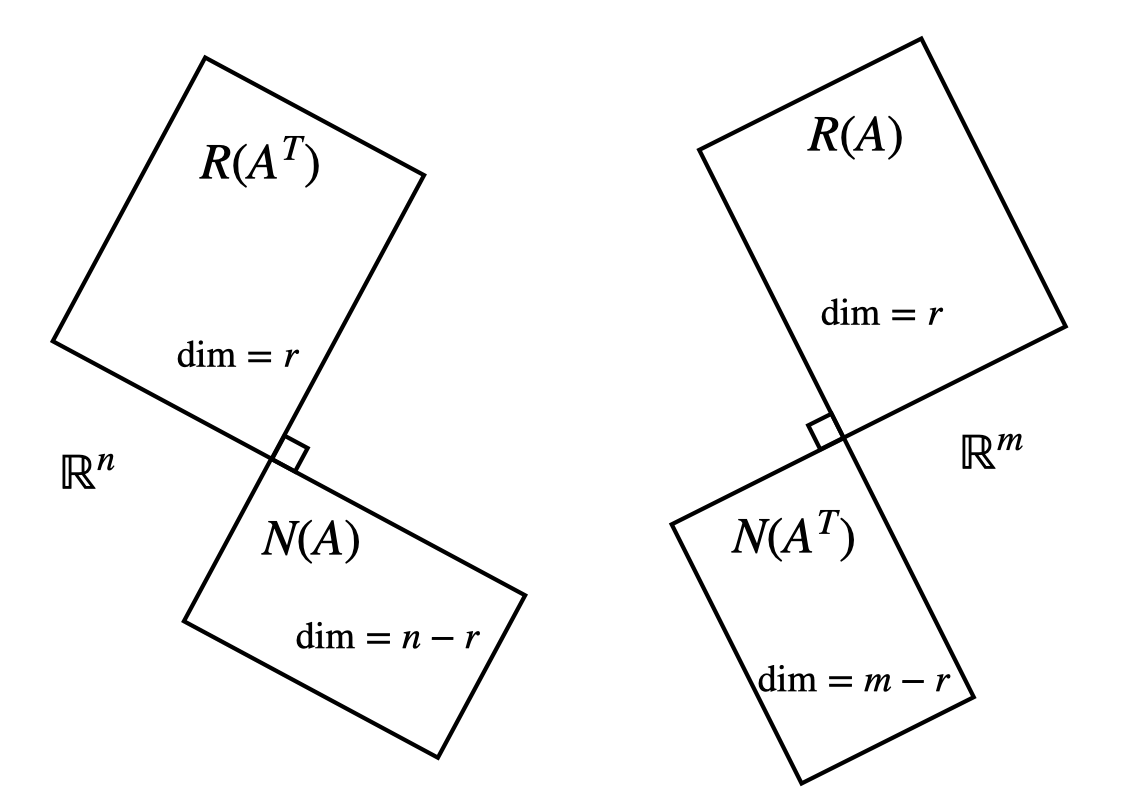
\includegraphics[width=0.55\linewidth]{figs/spaces.png}
\end{figure}
\end{remark}

\begin{definition}[正交变换]
设 $V$ 是一个欧式空间，$T$ 为其上的线性变换。若 $T$ 保持 $V$ 中任意向量 $x$ 长度不变，即 $\Vert Tx\Vert=\Vert x\Vert$，则称 $T$ 为正交变换。
\end{definition}

\begin{theorem}[正交变换的等价定义]
欧式空间 $V$ 上的线性变换 $T$ 是正交变换的充要条件是保持内积不变，即对任意 $x,y\in V$，有 $(Tx,Ty)=(x,y)$.
\end{theorem}

\begin{definition}[正交矩阵]
若方阵 $Q$ 满足：$Q^TQ=I$ 或 $Q^{-1}=Q^T$.  即 $Q$ 各列向量标准正交，则称 $Q$ 为正交矩阵。
\end{definition}

\begin{theorem}[正交变换与正交矩阵]
欧式空间上的线性变换 $T$ 为正交变换的充要条件是其在\textbf{标准正交基}下的矩阵表示是正交矩阵。
\end{theorem}
\begin{proof}
设 $X$ 为一个标准正交基，$TX=XA$，任取 $x=X\alpha$，则 $Tx=TX\alpha=XA\alpha$，因此：
\begin{align*}
    &(Tx,Tx)=(A\alpha)^T(A\alpha)=\alpha^TA^TA\alpha=(x,x)=\alpha^T\alpha\\
    \iff\;&\alpha^T(I-A^TA)\alpha=0\\
    \iff\;& A^TA=I
\end{align*}
\end{proof}
\begin{note}
注意定理成立必须是在标准正交基下。
\end{note}

\begin{property}
正交矩阵非奇异。
\end{property}

\begin{property}
正交矩阵的逆仍为正交矩阵。
\end{property}

\begin{property}
正交矩阵的乘积仍为正交矩阵。
\end{property}

\begin{property}
正交基变换矩阵为正交矩阵。
\end{property}
\begin{proof}
设 $X,Y$ 为正交基，$Y=XC$，任取 $x=Y\alpha=XC\alpha,\,y=Y\beta=XC\beta$，则：
\[
    (x,y)=\alpha^T\beta=(C\alpha)^T(C\beta)=\alpha^T(C^TC)\beta\implies C^TC=I
\]
\end{proof}

\begin{property}
正交矩阵的特征值位于复平面的单位圆上。
\end{property}
\begin{proof}
设 $A$ 为正交矩阵，$Ax=\lambda x\ (x\neq 0)$，则两边取共轭转置得 $x^HA^T=\bar\lambda x^H$（注意 $A$ 是实矩阵，但其特征值和特征向量可能是复数）。于是：
\[
    x^Hx=x^HA^TAx=\lambda\bar\lambda x^Hx=|\lambda|^2x^Hx\implies |\lambda|^2=1
\]
\end{proof}

\begin{definition}[线性映射的共轭]
设 $P$ 是欧氏空间 $W$ 到欧氏空间 $V$ 的一个线性映射，$Q$ 是 $V$ 到 $W$ 的一个线性映射，若对 $\forall x\in W,y\in V$，有 $(Px,y)=(x,Qy)$，则称 $Q$ 为 $P$ 的共轭。
\end{definition}

\begin{figure}[H]
    \centering
    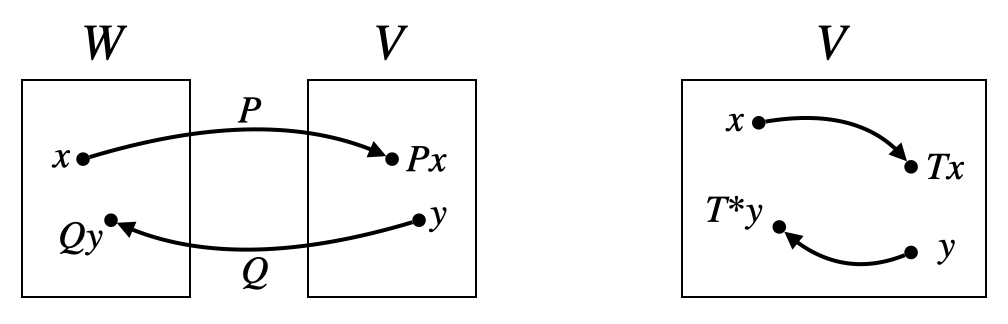
\includegraphics[width=0.5\linewidth]{figs/conj.png}
\end{figure}

\begin{theorem}
设 $X,Y$ 分别是欧式空间 $W,V$ 的标准正交基，$P$ 是 $W$ 到 $V$ 的一个线性映射，$Q$ 是 $P$ 的共轭。设 $P,Q$ 在 $X,Y$ 下的矩阵表示为 $A,B$，则 $B=A^T$.
\end{theorem}
\begin{proof}
由于 $PX=YA,\,QY=XB$，所以：
\begin{gather*}
    (Px_j,y_i)=\left(\sum_{k=1}^m a_{kj}y_k,y_i\right)=a_{ij}\\
    (x_j,Qy_i)=\left(x_j,\sum_{k=1}^nb_{ki}x_k\right)=b_{ji}
\end{gather*}
由于 $(Px_j,y_i)=(x_j,Qy_i)$，故 $a_{ij}=b_{ji}$，即 $B=A^T$.
\end{proof}

\begin{definition}[线性变换的共轭]
设 $T$ 是欧氏空间 $V$ 上的一个线性变换，若对 $\forall x,y\in V$，有 $(Tx,y)=(x,T^\ast y)$ 成立，则称 $T^\ast$ 为 $T$ 的共轭。
\end{definition}

\begin{theorem}
\label{thm:conjgram}
设 $T$ 在基 $X=(x_1,\ldots,x_n)$ 下的矩阵表示为 $A$，$X$ 的 Gram 矩阵为 $C$，那么 $T^\ast$ 在基 $X$ 下的矩阵表示为 $B=C^{-1}A^TC$.
\end{theorem}
\begin{proof}
由于 $TX=XA,\,T^\ast X=XB$，所以：
\begin{gather*}
    (Tx_i,x_j)=\left(\sum_{k=1}^na_{ki}x_k,x_j\right)=\sum_{k=1}^na_{ki}(x_k,x_j)=\sum_{k=1}^na_{ki}c_{kj}\\
    (x_i,T^\ast x_j)=\left(x_i,\sum_{k=1}^nb_{kj}x_k\right)=\sum_{k=1}^nb_{kj}(x_i,x_k)=\sum_{k=1}^nb_{kj}c_{ik}\\
\end{gather*}
得 $\sum_{k=1}^na_{ki}c_{kj}=\sum_{k=1}^n b_{kj}c_{ik}$，即 $A^TC=CB$.
\end{proof}

\begin{definition}[实对称变换]
设 $T$ 是欧氏空间 $V$ 的一个线性变换，且对 $V$ 中任意两个向量 $x,y$ 都有 $(Tx,y)=(x,Ty)$ 成立，则称 $T$ 为 $V$ 中一个实对称变换。
\end{definition}

\begin{theorem}[实对称变换与实对称矩阵]
欧氏空间中的线性变换是实对称变换的充要条件是它在\textbf{标准正交基}下的矩阵为实对称矩阵。
\end{theorem}
\begin{proof}
设 $X$ 为一个标准正交基，设 $T$ 在 $X$ 下的矩阵表示为 $A$，即 $TX=XA$.

必要性：由于 $X$ 为标准正交基，故其 Gram 矩阵为 $I$，由于 $T$ 本身就是自己的共轭，根据定理 \ref{thm:conjgram} 可知 $A=I^{-1}A^TI=A^T$.

充分性：
\begin{gather*}
(Tx_i,x_j)=\left(\sum_{k=1}^na_{ki}x_k,x_j\right)=a_{ji}\\
(x_i,Tx_j)=\left(x_i,\sum_{k=1}^na_{kj}x_k\right)=a_{ij}
\end{gather*}
得 $a_{ji}=a_{ij}$.
\end{proof}

\begin{theorem}
实对称矩阵特征值都为实数，属于不同特征值的特征向量相互正交。
\end{theorem}
\begin{proof}
设 $Ax=\lambda x\ (x\neq 0)$，则：
\[
x^HAx=\lambda x^Hx=(A^Hx)^Hx=(Ax)^Hx=(\lambda x)^Hx=\bar\lambda x^Hx\implies \lambda=\bar\lambda
\]
故 $\lambda\in\mathbb R$.
再设 $Ay=\mu y\ (y\neq 0)$ 且 $\lambda\neq \mu$，则：
\[
y^TAx=\lambda y^Tx=(A^Ty)^Tx=(Ay)^Tx=\mu y^Tx\implies y^Tx=0
\]
\end{proof}

下面我们将线性空间的数域从实数域扩展到复数域，那么相应的，欧式空间扩展为酉空间，内积扩展为复内积，正交变换和正交矩阵扩展为酉变换和酉矩阵，实对称变换和实对称矩阵扩展为 Hermite 矩阵和 Hermite 变换。它们都有着类似的性质。

\begin{definition}[复内积，酉空间]
设 $V$ 是复数域 $\mathbb C$ 上的线性空间，定义函数 $(\cdot,\cdot):V\times V\to \mathbb C$，若满足对 $\forall x,y,z\in V,\,c\in\mathbb C$，都有：
\begin{itemize}
    \item 非负性：$(x,x)\geq 0$
    \item 正定性：$(x,x)=0\iff x=0$
    \item 齐次性：$(cx,y)=c(x,y)$
    \item 分配律：$(x,y+z)=(x,y)+(x,z)$
    \item 共轭对称性：$(x,y)=\overline{(y,x)}$
\end{itemize}
则称 $(\cdot,\cdot)$ 为复内积，$V$ 为酉空间、复欧氏空间或复内积空间。
\end{definition}

\begin{example}[根据坐标定义复内积]
设 $X$ 为 $V$ 上的一个基，向量 $x,y\in V$ 在该基下的坐标分别为 $\alpha=(\alpha_1,\ldots,\alpha_n)^T,\beta=(\beta_1,\ldots,\beta_n)^T$，则可以定义内积为：
\[
    (x,y)=\alpha_1\bar\beta_1+\cdots+\alpha_n\bar\beta_n=\beta^H\alpha
\]
容易验证这确实满足内积的四个条件。
\end{example}
\begin{note}
注意共轭转置取在 $\beta$ 上，这是为了满足齐次性而导致的。在有些教材上，齐次性写作 $(x,cy)=c(x,y)$，则内积相应地会变成 $\alpha^H\beta$，共轭转置取在 $\alpha$ 上。
\end{note}

注意 Cauchy-Schwarz 不等式 \ref{thm:cauchy-schwarz}、三角不等式 \ref{thm:triangle} 和平行四边形恒等式 \ref{thm:parallelogram} 的证明过程对复内积仍然适用，因此它们对复内积仍然成立。

\begin{theorem}[极化恒等式]
\label{thm:polirization}
\[
    \text{Re}(x,y)=\frac{1}{4}\left(\norm{x+y}^2-\norm{x-y}^2\right)
\]
\end{theorem}
\begin{proof}
\begin{align*}
    \norm{x+y}^2-\norm{x-y}^2&=\big(\norm{x}^2+\norm{y}^2+(x,y)+(y,x)\big)-\big(\norm{x}^2+\norm{y}^2-(x,y)-(y,x)\big)\\
    &=2(x,y)+2(y,x)=4\text{Re}(x,y)
\end{align*}
\end{proof}

\begin{definition}[酉变换]
设 $T$ 是酉空间 $V$ 中的线性变换，若 $T$ 保持长度不变，即对 $V$ 中任意 $x$，有 $(Tx,Tx)=(x,x)$，则称 $T$ 为 $V$ 上的酉变换。
\end{definition}

\begin{theorem}[酉变换的等价定义]
酉空间 $V$ 上的线性变换 $T$ 是酉变换的充要条件是保持内积不变，即对任意 $x,y\in V$，有 $(Tx,Ty)=(x,y)$.
\end{theorem}

\begin{definition}[酉矩阵]
若 $n$ 阶矩阵 $A$ 满足 $A^HA=AA^H=I$，则称 $A$ 为酉矩阵。
\end{definition}

\begin{theorem}[酉变换与酉矩阵]
酉变换在酉空间的\textbf{标准正交基}下的矩阵是酉矩阵。
\end{theorem}

\begin{property}
酉矩阵的逆矩阵也是酉矩阵。
\end{property}

\begin{property}
两个酉矩阵的乘积也是酉矩阵。
\end{property}

\begin{definition}[复线性映射的共轭]
设 $P$ 是酉空间 $W$ 到酉空间 $V$ 的一个线性映射，$Q$ 是酉空间
$V$ 到酉空间 $W$ 的一个线性映射，若对 $\forall x\in W,y\in V$，有 $(Px,y)=(x,Qy)$，则称 $Q$ 为 $P$ 的共轭。
\end{definition}

\begin{theorem}
设 $X,Y$ 分别是酉空间 $W,V$ 的标准正交基，$P$ 是 $W$ 到 $V$ 的一个线性映射，$Q$ 是 $P$ 的共轭。设 $P,Q$ 在 $X,Y$ 下的矩阵表示为 $A,B$，则 $B=A^H$.
\end{theorem}

\begin{definition}[复线性变换的共轭]
设 $T$ 是酉空间 $V$ 上的一个线性变换，若对 $\forall x,y\in V$，有 $(Tx,y)=(x,T^\ast y)$ 成立，则称 $T^\ast$ 为 $T$ 的共轭。
\end{definition}

\begin{property}
线性变换 $T$ 的共轭仍是线性变换。
\end{property}
\begin{theorem}
设 $T$ 在基 $X=(x_1,\ldots,x_n)$ 下的矩阵表示为 $A$，$X$ 的 Gram 矩阵为 $C$，那么 $T^\ast$ 在基 $X$ 下的矩阵表示为 $B=C^{-1}A^HC$.
\end{theorem}

\begin{definition}[Hermite 变换/酉对称变换]
设 $T$ 为酉空间 $V$ 上的线性变换，若满足对任意 $x,y\in V$，都有 $(Tx,y)=(x,Ty)$，则称 $T$ 为 Hermite 变换或酉对称变换。
\end{definition}

\begin{definition}[Hermite 矩阵]
若 $n$ 阶矩阵 $A$ 满足 $A=A^H$，则称 $A$ 为 Hermite 矩阵。
\end{definition}

\begin{theorem}[Hermite 变换与 Hermite 矩阵]
Hermite 变换在\textbf{标准正交基}下的矩阵是 Hermite 矩阵。
\end{theorem}

\begin{theorem}
Hermite 矩阵的特征值都是实数，属于不同特征值的特征向量相互正交。
\end{theorem}

\begin{theorem}[Schur 定理]
\label{thm:schur}
\ 

1) 设 $A\in\mathbb C^{n\times n}$，则存在酉矩阵 $P$ 使得 $P^HAP=U$，其中 $U$ 为上三角矩阵。

2) 设 $A\in\mathbb R^{n\times n}$ 且所有特征值为实数，则存在正交矩阵 $Q$ 使得 $Q^TAQ=U$，其中 $U$ 为上三角矩阵。
\end{theorem}

\begin{remark}
在定理 \ref{thm:anysimilar} 中，我们证明了任意矩阵都相似于一个上三角矩阵。Schur 定理是该定理的加强版，它限制用来相似化的矩阵是一个酉矩阵。Schur 定理的证明过程与定理 \ref{thm:anysimilar} 是类似的，只不过基扩充时需要扩充为标准正交基，所有的可逆矩阵换成酉矩阵。
\end{remark}

\begin{definition}[正规矩阵]
设 $A\in\mathbb C^{n\times n}$ 且 $A^HA=AA^H$，称 $A$ 为正规矩阵。
\end{definition}
\begin{remark}
式 $A^HA=AA^H$ 意味着 $A$ 的 $i,j$ 行内积等于 $i,j$ 列内积。因此，前面提到的\textbf{正交矩阵、对称矩阵、酉矩阵、Hermite 矩阵都是正规矩阵}。
\end{remark}

\begin{theorem}[正规矩阵的充要条件]
\label{thm:unisim}
\ 

1) 设 $A\in\mathbb C^{n\times n}$，则 $A$ 为正规矩阵的充要条件为 $A$ 酉相似于对角矩阵，即存在酉矩阵 $P$ 使得 $P^HAP=D$，其中 $D$ 为对角矩阵。

2) 设 $A\in\mathbb R^{n\times n}$ 且所有特征值为实数，则 $A$ 为正规矩阵的充要条件为 $A$ 正交相似于对角矩阵，即存在正交矩阵 $Q$ 使得 $Q^TAQ=D$，其中 $D$ 为对角矩阵。
\end{theorem}
\begin{proof}
只证明 1)，2) 类似可证。充分性易证；对于必要性，根据 Schur 定理 \ref{thm:schur}，$A$ 酉相似于一个上三角矩阵：$P^HAP=U$. 容易证明，$A$ 正规 $\iff$ $U$ 正规，于是 $U^HU=UU^H$，故 $U$ 只能是对角矩阵。
\end{proof}

\begin{corollary}
实对称矩阵正交相似于对角矩阵。
\end{corollary}

% \begin{theorem}[Hermite 矩阵的谱分解]
% 设 $A$ 为 Hermite 矩阵，$\lambda_i,p_i$ 是 $A$ 的特征值和特征向量，则：
% \[
%     A=\lambda_1p_1p_1^H+\cdots+\lambda_np_np_n^H=P\Lambda P^H
% \]
% \end{theorem}
 \newpage
\section{范数理论及其应用}

\subsection{向量范数}

\begin{definition}[向量范数]
设 $V$ 是数域 $\mathbb F$ ($\mathbb R$ 或 $\mathbb C$) 上的线性空间，定义实值函数 $\norm \cdot:V\to\mathbb R$，若满足对 $\forall x,y\in V,\,c\in\mathbb F$，都有：
\begin{enumerate}
    \item 非负性：$\norm x\geq0$
    \item 正定性：$\norm{x}=0\iff x=0$
    \item 齐次性：$\norm{cx}=|c|\norm{x}$
    \item 三角不等式：$\norm{x+y}\leq\norm{x}+\norm{y}$
\end{enumerate}
则称 $\norm{\cdot}$ 为 $V$ 上的一个范数。
\end{definition}
\begin{com}
$|c|$ 表示 $c$ 的绝对值（$\mathbb F=\mathbb R$）或模（$\mathbb F=\mathbb C$）。
\end{com}

\begin{remark}
在第一章中，由定义 \ref{def:inner-product-norm} 给出的范数称作由内积诱导的范数。而根据上述范数的公理化定义，范数并不一定是由内积诱导而来的，只需满足上述四条要求即可。事实上，可以证明平行四边形恒等式 \ref{thm:parallelogram} 是一个范数可以由内积诱导而来的充要条件。
\end{remark}

\begin{theorem}[由内积诱导的范数]
定义 \ref{def:inner-product-norm} 给出的由内积诱导的范数的确是一个范数。
\end{theorem}
\begin{proof}
根据内积的非负性、正定性和齐次性，容易推出由内积诱导的范数满足非负性、正定性和齐次性。又根据定理 \ref{thm:triangle} 知三角不等式成立，故由内积诱导的范数的确满足范数的公理化定义。
\end{proof}

\begin{theorem}
$\forall x,y\in V,\,\left|\norm x-\norm y\right|\leq\norm{x-y}$.
\end{theorem}
\begin{proof}
$\Vert x\Vert=\norm{(x-y)+y}\leq\norm{x-y}+\norm y$. 另一方向同理。
\end{proof}

\begin{theorem}[范数是凸函数]
对 $0\leq\lambda\leq1$，有 $\norm{(1-\lambda)x+\lambda y}\leq(1-\lambda)\norm x+\lambda\norm y$.
\end{theorem}
\begin{proof}
由三角不等式与齐次性容易推出。
\end{proof}

\begin{theorem}[范数的乘法]
若 $\norm{\cdot}$ 是 $V$ 上的向量范数，则 $c\norm{\cdot}$ 仍然为向量范数，其中 $c>0$.
\end{theorem}
\begin{proof}
容易验证 $c\norm{\cdot}$ 仍然满足范数的四条要求。
\end{proof}

\begin{theorem}[范数的复合]
设 $\norm{\cdot}_\text{comp}$ 是 $\mathbb R^m$ 上的范数，且对 $x\in(\mathbb R^+)^m$ 为单调增加的。那么，给定 $m$ 个 $n$ 维线性空间 $V$ 上的范数 $\norm{\cdot}_i\,(i=1,\ldots,m)$，可以定义复合范数为：
\[
    \norm{x}=\norm{U(x)}_\text{comp},\quad \text{where }\ U(x)=(\norm{x}_1,\ldots,\norm{x}_m)^T
\]
\end{theorem}
\begin{proof}
非负性、正定性和齐次性是显然的，下面证明三角不等式。
\begin{align*}
    \norm{x+y}&=\norm{U(x+y)}_\text{comp}\\
    &\leq\norm{U(x)+U(y)}_\text{comp}\\
    &\leq\norm{U(x)}_\text{comp}+\norm{U(y)}_\text{comp}\\
    &=\norm{x}+\norm{y}
\end{align*}
其中第二行是因为 $U(x+y)\leq U(x)+U(y)$，且 $\norm{\cdot}_\text{comp}$ 单调增加。
\end{proof}

\begin{example}
设 $\norm\cdot_f$ 和 $\norm\cdot_g$ 是线性空间 $V$ 上的两个向量范数，则：
\begin{enumerate}
    \item $\norm\cdot_f+\norm\cdot_g$ 是 $V$ 上的向量范数
    \item $\max\{\norm\cdot_f,\norm\cdot_g\}$ 是 $V$ 上的向量范数
    \item $\left[(\norm\cdot_f)^2+(\norm\cdot_g)^2\right]^{1/2}$ 是 $V$ 上的向量范数
\end{enumerate}
\end{example}

\begin{theorem}[范数的合成]
设 $n$ 维线性空间 $V=V_1\oplus V_2\oplus\cdots\oplus V_m$，且 $\norm\cdot_i\,(i=1,\ldots,m)$ 为线性子空间 $V_i$ 上的范数。设 $\norm{\cdot}_\text{comp}$ 是 $\mathbb R^m$ 上的范数，且对 $x\in\mathbb (R^+)^m$ 为单调增加的，则对任意 $x\in V$，存在唯一分解 $x=x_1+\cdots+x_n$，其中 $x_i\in V_i$.  定义合成范数为：  
\[
    \norm x=\norm{U(x)}_\text{comp},\quad\text{where }\ U(x)=(\norm{x_1}_1,\ldots,\norm{x_m}_m)^T
\]
\end{theorem}

下面的定义与定理给出了范数的几何性质。

\begin{definition}[均衡闭凸集]
线性空间 $V$ 的闭凸集 $\Omega$ 若满足：$x\in\Omega\implies \lambda x\in\Omega\,(|\lambda|\leq1)$，那么称 $\Omega$ 为均衡闭凸集。
\end{definition}

\begin{theorem}[范数与均衡闭凸集一一对应]
若 $\norm\cdot$ 为 $V$ 上的向量范数，则 $\Omega=\{x\mid\norm x\leq 1\}$ 是 $V$ 上的均衡闭凸集；反之，若 $\Omega$ 是 $V$ 上的均衡闭凸集，且 $\Omega$ 含有内点，则可以定义函数 $P(x)$ 如下：
\[
    P(x)=\begin{cases}\min\{\lambda>0\mid x/\lambda\in\Omega\}&x\neq0\\0&x=0\end{cases}
\]
那么 $P(x)$ 为 $V$ 上的范数。
\end{theorem}

下面给出几个 $\mathbb C^n$ 上的常用范数。

\begin{example}[2-范数]
\[
    \norm x_2=\sqrt{|x_1|^2+|x_2|^2+\cdots+|x_n|^2}
\]
\end{example}

\begin{example}[1-范数]
\[
    \norm x_1=|x_1|+|x_2|+\cdots+|x_n|
\]
\end{example}

\begin{example}[$\infty$-范数]
\[
    \norm x_\infty=\max_{i=1}^n |x_i|
\]
\end{example}

\begin{example}[$p$-范数]
\[
    \norm x_p=\left(|x_1|^p+|x_2|^p+\cdots+|x_n|^p\right)^{1/p}\quad\quad p\geq 1
\]
\end{example}

\begin{remark}
当 $0\leq p<1$ 时并不是范数，因为不满足三角不等式，但是在实际应用中仍然有重要应用。    
\end{remark}

\begin{figure}[H]
    \centering
    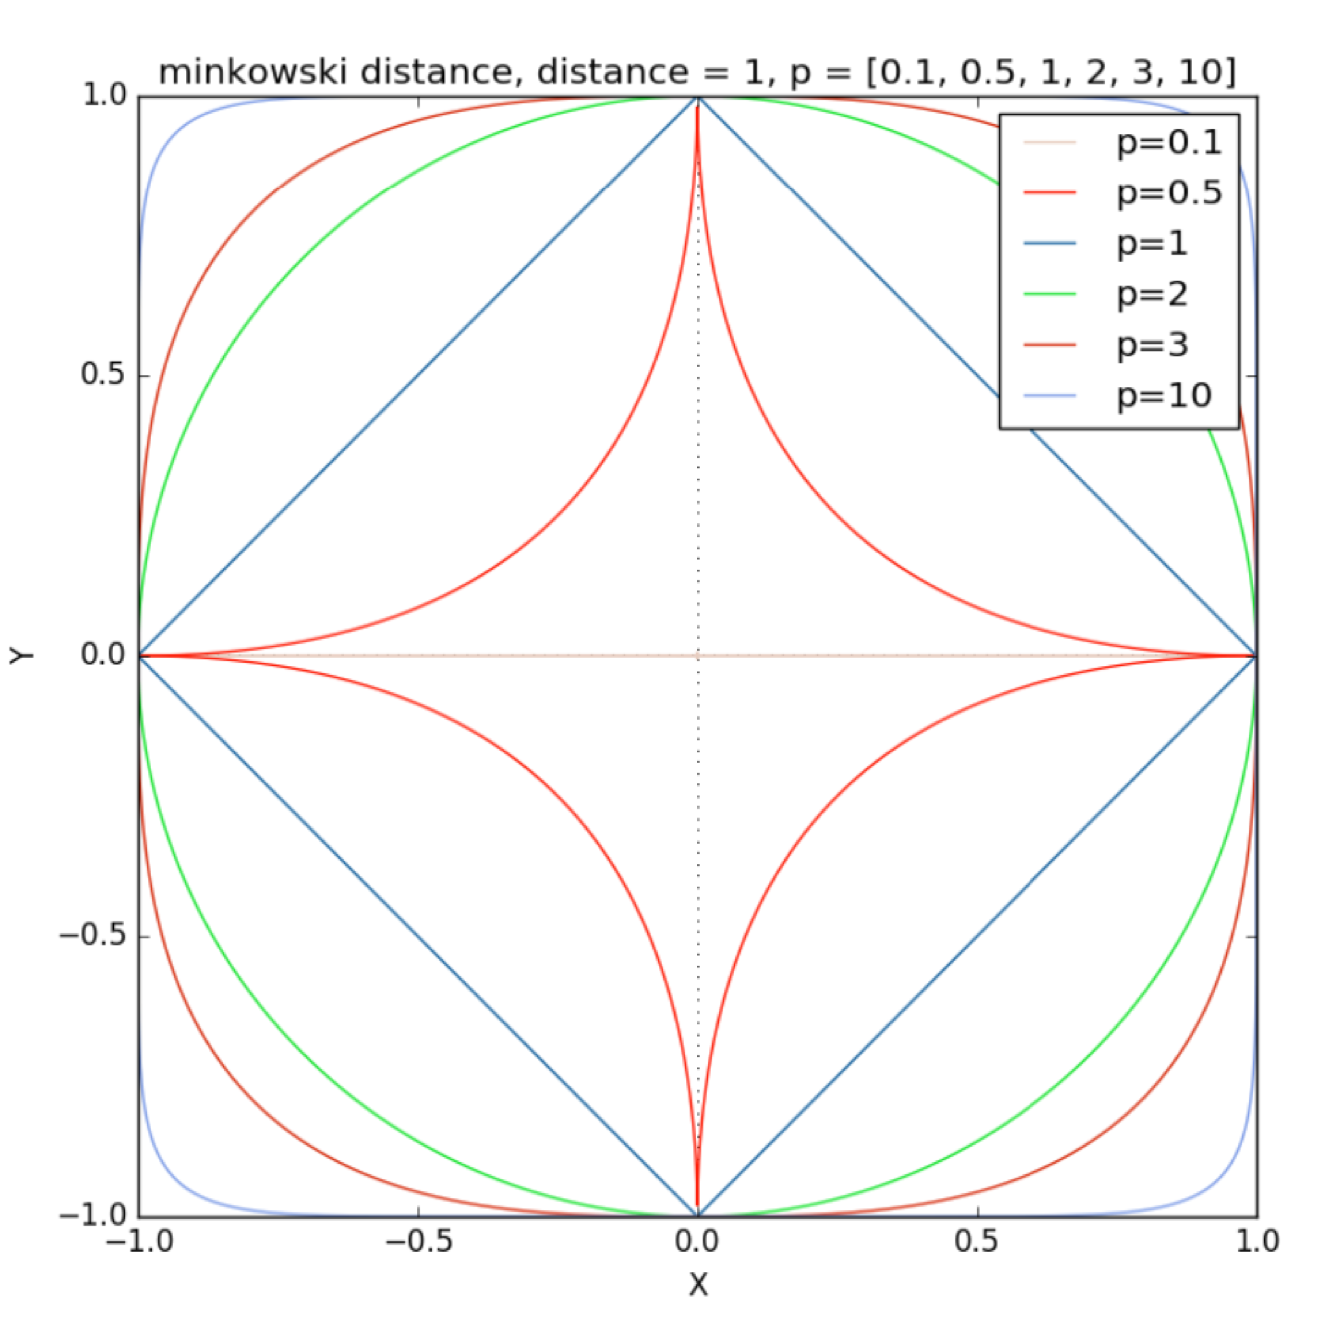
\includegraphics[width=0.5\linewidth]{figs/pnorm.png}
\end{figure}

为了证明 $p$-范数在 $p\geq 1$ 时满足三角不等式，首先需要证明一个引理和 Hölder 不等式。

\begin{lemma}
对任意实数 $\alpha>0,\beta>0$，都有 $\alpha\beta\leq \frac{\alpha^p}{p}+\frac{\beta^q}{q}$，其中 $p>1,q>1$ 且 $\frac{1}{p}+\frac{1}{q}=1$.
\end{lemma}
\begin{proof}
\begin{align*}
    \frac{\alpha^p}{p}+\frac{\beta^q}{q}&\geq\frac{q\alpha^p+p\beta^q}{pq}=\frac{q\alpha^p+p\beta^q}{p+q}\\
    &=\frac{(\alpha^p+\cdots+\alpha^p)+(\beta^q+\cdots+\beta^q)}{p+q}\\
    &\geq\sqrt[p+q]{\alpha^{pq}\beta^{pq}}=\sqrt[pq]{\alpha^{pq}\beta^{pq}}=\alpha\beta
\end{align*}
\end{proof}

\begin{theorem}[Hölder 不等式]
对任意 $\xi_k,\eta_k\in\mathbb C\,(k=1,\ldots,n)$，有：
\[
    \sum_{k=1}^n|\xi_k||\eta_k|\leq\left(\sum_{k=1}^n|\xi_k|^p\right)^{1/p}\left(\sum_{k=1}^n|\eta_k|^q\right)^{1/q}
\]
其中 $p>1,q>1$ 且 $\frac{1}{p}+\frac{1}{q}=1$.
\end{theorem}
\begin{proof}
令 $\alpha={|\xi_i|}/{\left(\sum_{k=1}^n|\xi_k|^p\right)^{1/p}}$，$\beta={|\eta_i|}/{\left(\sum_{k=1}^n|\eta_k|^q\right)^{1/q}}$，由引理得：
\[
    \frac{|\xi_i|}{\left(\sum_{k=1}^n|\xi_k|^p\right)^{1/p}}\cdot\frac{|\eta_i|}{\left(\sum_{k=1}^n|\eta_k|^q\right)^{1/q}}\leq\frac{|\xi_i|^p}{p\sum_{k=1}^n|\xi_k|^p}+\frac{|\eta_i|^q}{q\sum_{k=1}^n|\eta_k|^q}
\]
对 $i$ 求和：
\[
    \frac{\sum_{i=1}^n|\xi_i||\eta_i|}{\left(\sum_{k=1}^n|\xi_k|^p\right)^{1/p}\left(\sum_{k=1}^n|\eta_k|^q\right)^{1/q}}\leq\frac{1}{p}+\frac{1}{q}=1
\]
\end{proof}

接下来利用 Hölder 不等式就可以证明 $p$-范数满足三角不等式了。

\begin{proof}
设 $x,y\in\mathbb C^n$，当 $p\geq 1$ 时，有：
\begin{align*}
    \norm{x+y}_p^p&=\sum_{k=1}^n|x_k+y_k|^p\\
    &\leq\sum_{k=1}^n|x_k||x_k+y_k|^{p-1}+\sum_{k=1}^n|y_k||x_k+y_k|^{p-1}\\
    &\leq\left(\sum_{k=1}^n|x_k|^p\right)^{1/p}\left(\sum_{k=1}^n|x_k+y_k|^{q(p-1)}\right)^{1/q}\\&+\left(\sum_{k=1}^n|y_k|^p\right)^{1/p}\left(\sum_{k=1}^n|x_k+y_k|^{q(p-1)}\right)^{1/q}\\
    &=\left(\norm{x}_p+\norm{y}_p\right)\left(\sum_{k=1}^n|x_k+y_k|^{p}\right)^{1/q}\\
    &=\left(\norm{x}_p+\norm{y}_p\right)\norm{x+y}_p^{p/q}\\
    &=\left(\norm{x}_p+\norm{y}_p\right)\norm{x+y}_p^{p-1}
\end{align*}
于是：
\[
    \norm{x+y}_p\leq\left(\norm{x}_p+\norm{y}_p\right)
\]
\end{proof}

\begin{definition}[绝对范数，单调范数]
设 $x=(\xi_1,\ldots,\xi_n)^T\in\mathbb F^n$，记 $|x|=(|\xi_1|,\ldots,|\xi_n|)^T\in\mathbb R^n$，则称 $\mathbb F^n$ 上的范数 $v$ 为：
\begin{itemize}
    \item 绝对范数，若满足 $v(x)=v(|x|),\quad \forall x\in\mathbb F^n$；
    \item 单调范数，若满足 $|x|\leq |y|\implies v(x)\leq v(y),\quad \forall x,y\in\mathbb F^n$.
\end{itemize}
\end{definition}

\begin{theorem}
$\mathbb F^n$ 上的范数 $v$ 为绝对范数的充要条件是 $v$ 为单调范数。
\end{theorem}
\begin{proof}
充分性：设 $v$ 为单调范数，则对于任意 $x\in\mathbb F^n$，令 $y=|x|$，由于 $|x|\leq |y|$ 且 $|y|\geq|x|$，所以 $v(x)\leq v(y)$ 且 $v(y)\leq v(x)$，故 $v(x)=v(y)$，即 $v$ 为绝对范数。

必要性：设 $v$ 为绝对范数，则对于任意给定 $x\in\mathbb F^n$，任取 $k\in\{1,\ldots,n\}$，设 $\alpha\in[0,1]$，考察向量 $[x_1,\ldots,x_{k-1},\alpha x_k,x_{k+1},\ldots,x_n]^T$ 的范数，有：
\begin{align*}
    &v([x_1,\ldots,x_{k-1},\alpha x_k,x_{k+1},\ldots,x_n]^T)\\
    =\;&v\left(\frac{1-\alpha}{2}[x_1,\ldots,x_{k-1},-x_k,x_{k+1},\ldots,x_n]^T+\frac{1-\alpha}{2}x+\alpha x\right)\\
    \leq\;&\frac{1-\alpha}{2}v\left([x_1,\ldots,x_{k-1},-x_k,x_{k+1},\ldots,x_n]^T\right)+\frac{1-\alpha}{2}v(x)+\alpha v(x)\\
    =\;&\frac{1-\alpha}{2}v(x)+\frac{1-\alpha}{2}v(x)+\alpha v(x)=v(x)
\end{align*}
对各个分量反复应用上式，则对任意 $x\in\mathbb F^n$ 及任意 $\alpha_1,\ldots,\alpha_n\in[0,1]$，都有：
\[
    v([\alpha_1x_1,\ldots,\alpha_nx_n]^T)\leq v(x)
\]
最后，对 $\forall x,y\in\mathbb F^n$ 且 $\Vert x\Vert\leq\Vert y\Vert$，考虑每一个分量，存在 $\alpha_k\in[0,1]$ 和 $\theta_k$ 使得 $x_k=\alpha_ke^{i\theta_k}y_k$，因此：
\[
    v(x)=v([\alpha_1e^{i\theta_1}y_1,\ldots,\alpha_ne^{i\theta_n}y_n]^T)=v([\alpha_1|y_1|,\ldots,\alpha_n|y_n|]^T)\leq v(y)
\]
即 $v$ 是单调范数。
\end{proof}

\begin{definition}[对偶范数]
令 $\norm\cdot$ 为 $\mathbb R^n$ 上的范数，其对偶范数 $\norm\cdot^\ast$ 定义为：
\[
    \norm{z}^\ast=\sup_{\norm x\leq 1}\{z^Tx\}
\]
\end{definition}

\begin{property}
对偶范数的对偶是其本身，即 $\norm{x}^{\ast\ast}=\norm x$.
\end{property}

\begin{example}
$l_p$ 和 $l_q$ 互为对偶范数，其中 $\frac{1}{p}+\frac{1}{q}=1$.
\end{example}

\begin{definition}[范数等价]
对有限维空间 $V^n$ 中任意两个向量范数 $\norm x_\alpha,\norm x_\beta$，若存在正常数 $c_1,c_2$，使得：
\[
    c_1\norm{x}_\beta\leq\norm{x}_\alpha\leq c_2\norm{x}_\beta,\quad\forall x\in V^n
\]
则称范数 $\norm{x}_\alpha$ 与 $\norm{x}_\beta$ 等价。
\end{definition}
\begin{com}
范数等价是一个\textbf{等价关系}，即满足\textbf{自反性、对称性、传递性}。
\end{com}

\begin{theorem}
有限维空间中任意两个向量范数都等价。
\end{theorem}
\begin{proof}
由于等价关系具有传递性，我们只需要证明任意一个向量范数都等价于 2-范数即可。
令 $f(x)=\norm{x}$ 为 $V^n$ 上的任一向量范数，由于当 $x\to y$ 时，$\left|\norm x-\norm y\right|\leq \norm{x-y}\to 0$，因此范数是连续函数。于是 $f(x)$ 在单位超球面上有大于零的最小值和最大值：
\[
    0<\min_{\norm{x}_2=1}f(x)\leq \max_{\norm{x}_2=1}f(x)
\]
记上述最小值为 $c_1$，最大值为 $c_2$，于是：
\[
    c_1\leq \left\Vert\frac{x}{\norm{x}_2}\right\Vert\leq c_2\implies c_1\norm{x}_2\leq\norm{x}\leq c_2\norm{x}_2
\]
故 $\norm\cdot$ 与 2-范数等价。
\end{proof}

\begin{definition}[依范数收敛]
设 $\{x^{(k)}\}$ 是 $V^n$ 中的向量序列，若存在 $x\in V^n$，使得：
\[
    \lim_{k\to\infty} \norm{x^{(k)}-x}_\alpha=0
\]
则称序列 $\{x^{(k)}\}$ 依 $\alpha$ 范数收敛到 $x$.
\end{definition}

\begin{theorem}
向量序列各分量收敛等价于依范数收敛，即：
\[
    \lim_{k\to\infty} x^{(k)}=x\iff\lim_{k\to\infty} \norm{x^{(k)}-x}=0
\]
\end{theorem}
\begin{proof}
由于向量范数的等价性，只需要对 1-范数证明即可。
\begin{align*}
    x^{(k)}\to x&\iff \xi_i^{(k)}\to\xi_i,\quad i=1,\ldots,n\\
    &\iff |\xi_i^{(k)}-\xi_i|\to 0,\quad i=1,\ldots,n\\
    &\iff \sum_{i=1}^n|\xi_i^{(k)}-\xi_i|\to 0\\
    &\iff \norm{x^{(k)}-x}_1\to0
\end{align*}
\end{proof}

\subsection{矩阵范数}

\begin{definition}[广义矩阵范数]
与向量范数相同，满足 3 条性质：
\begin{enumerate}[series=matrix-norm]
    \item 非负性：$\norm{A}\geq 0$ 且 $\norm{A}=0\iff A=0$
    \item 齐次性：$\norm{kA}=|k|\norm{A},\,k\in K$
    \item 三角不等式：$\norm{A+B}\leq\norm{A}+\norm{B}$
\end{enumerate}
\end{definition}

\begin{definition}[矩阵范数]
在广义矩阵范数的基础上增加相容条件：
\begin{enumerate}[resume=matrix-norm]
    \item 相容性：$\norm{AB}\leq\norm{A}\norm{B}$
\end{enumerate}
\end{definition}

\begin{remark}
对于涉及到矩阵范数的不等式放缩，一般就是考虑三角不等式和相容性。
\end{remark}

\begin{definition}[相容范数]
对 $\mathbb C^{m\times n}$ 上的矩阵范数 $\norm{A}_M$ 和 $\mathbb C^m,\mathbb C^n$ 上的同类向量范数 $\norm{x}_v$，若：
\[
    \norm{Ax}_v\leq \norm{A}_M\norm{x}_v,\quad \forall A\in\mathbb C^{m\times n},\,\forall x\in\mathbb C^n
\]
则称矩阵范数 $\norm{A}_M$ 与向量范数 $\norm{x}_v$ 是相容的。
\end{definition}

\begin{remark}
简单地说，把矩阵视作线性映射，则相容范数表示，映射后的向量与原向量的长度的相对变化量被矩阵范数所控制。
\end{remark}

\begin{example}[$m_1$ 范数]
设 $A\in\mathbb C^{m\times n}$，矩阵的 $m_1$ 范数与向量的 1-范数定义类似：
\[
    \norm{A}_{m_1}=\sum_{i=1}^m\sum_{j=1}^n|a_{ij}|
\]
即所有元素的绝对值（模）之和。可以证明 \textbf{$m_1$ 范数是矩阵范数，并且与向量的 1-范数相容}。
\end{example}

\begin{proof}
非负性、齐次性和三角不等式与向量的 1-范数完全相同，必然成立，只需证明矩阵范数的相容性以及与向量 1-范数的相容性。

相容性：
\begin{align*}
    \norm{AB}_{m_1}&=\sum_{i=1}^m\sum_{j=1}^l\left|\sum_{k=1}^na_{ik}b_{kj}\right|\\
    &\leq\sum_{i=1}^m\sum_{j=1}^l\sum_{k=1}^n|a_{ik}||b_{kj}|\\
    &\leq\sum_{k=1}^n\left[\left(\sum_{i=1}^m|a_{ik}|\right)\left(\sum_{j=1}^l|b_{kj}|\right)\right]\\
    &\leq\left(\sum_{k=1}^n\sum_{i=1}^m|a_{ik}|\right)\left(\sum_{k=1}^n\sum_{j=1}^l|b_{kj}|\right)\\
    &=\norm{A}_{m_1}\norm{B}_{m_1}
\end{align*}

与向量的 1-范数相容：
\begin{align*}
    \norm{Ax}_1&=\sum_{i=1}^m\left|\sum_{j=1}^na_{ij}x_j\right|\\
    &\leq\sum_{i=1}^m\sum_{j=1}^n|a_{ij}||x_j|\\
    &\leq\left(\sum_{i=1}^m\sum_{j=1}^n|a_{ij}|\right)\left(\sum_{j=1}^n|x_j|\right)\\
    &=\norm{A}_{m_1}\norm{x}_1
\end{align*}    
\end{proof}

\begin{definition}[$m_\infty$ 范数]
设 $A\in\mathbb C^{m\times n}$，矩阵的 $m_\infty$ 范数与向量的无穷范数定义类似，\textbf{但是要乘以 $n$}，否则不满足相容性：
\[
    \norm{A}_{m_\infty}=n\cdot\max_{i,j}|a_{ij}|
\]
可以证明 \textbf{$m_\infty$ 范数是矩阵范数，且与向量的无穷范数相容}。
\end{definition}
\begin{proof}
相容性：
\begin{align*}
\norm{AB}_{m_\infty}&=n\cdot\max_{i,j}\left|\sum_{k=1}^n a_{ik}b_{kj}\right|\\
&\leq n\cdot\max_{i,j}\sum_{k=1}^n |a_{ik}||b_{kj}|\\
&\leq n\cdot\max_{i,j}\left[n\cdot(\max_k |a_{ik}|)(\max_k |b_{kj}|)\right]\\
&=\max_{i,j}\left[(n\cdot \max_k |a_{ik}|)(n\cdot\max_k |b_{kj}|)\right]\\
&=(n\cdot \max_{i,k} |a_{ik}|)(n\cdot\max_{k,j} |b_{kj}|)\\
&=\norm{A}_{m_\infty}\norm{B}_{m_\infty}
\end{align*}

与向量的无穷范数相容：
\begin{align*}
\norm{Ax}_{\infty}&=\max_i\left|\sum_{j=1}^na_{ij}x_j\right|\\
&\leq\max_i\sum_{j=1}^n|a_{ij}||x_j|\\
&\leq\max_i\left[n\cdot(\max_j |a_{ij}|)(\max_j |x_j|)\right]\\
&=n\cdot\max_{i,j}|a_{ij}|\cdot\max_j |x_j|\\
&=\norm{A}_{m_\infty}\norm{x}_{\infty}
\end{align*}
\end{proof}

\begin{definition}[Frobenius 范数]
设 $A\in\mathbb C^{m\times n}$，矩阵的 F-范数与向量的 2-范数定义类似：
\[
    \norm{A}_{F}=\norm{A}_{m_2}=\left(\sum_{i=1}^m\sum_{j=1}^n|a_{ij}|^2\right)^{1/2}=\left(\text{tr}(A^HA)\right)^{1/2}
\]
可以证明 \textbf{F-范数是矩阵范数，并且与向量的 2-范数相容}。
\end{definition}
\begin{proof}
相容性：
\begin{align*}
\norm{AB}_F^2&=\sum_{i=1}^m\sum_{j=1}^l\left|\sum_{k=1}^na_{ik}b_{kj}\right|^2\\
&\leq\sum_{i=1}^m\sum_{j=1}^l\left(\sum_{k=1}^n|a_{ik}||b_{kj}|\right)^2\\
&\leq\sum_{i=1}^m\sum_{j=1}^l\left(\sum_{k=1}^n|a_{ik}|\right)^2\left(\sum_{k=1}^n|b_{kj}|\right)^2\\
&\leq\left(\sum_{i=1}^m\sum_{k=1}^n|a_{ik}|\right)^2\left(\sum_{j=1}^l\sum_{k=1}^n|b_{kj}|\right)^2\\
&=\norm{A}_F^2\norm{B}_F^2
\end{align*}

与向量的 2-范数相容：
\begin{align*}
\norm{Ax}_2^2&=\sum_{i=1}^m\left|\sum_{j=1}^n a_{ij}x_j\right|^2\\
&\leq\sum_{i=1}^m\left(\sum_{j=1}^n |a_{ij}||x_j|\right)^2\\
&\leq\sum_{i=1}^m\left(\sum_{j=1}^n |a_{ij}|\right)^2\left(\sum_{j=1}^n|x_j|\right)^2\\
&\leq\left(\sum_{i=1}^m\sum_{j=1}^n |a_{ij}|\right)^2\left(\sum_{j=1}^n|x_j|\right)^2\\
&=\norm{A}_F^2\norm{x}_2^2
\end{align*}
\end{proof}

\begin{theorem}[Frobenius 范数的酉不变性]
设 $A\in\mathbb C^{m\times n}$，酉矩阵 $P\in\mathbb C^{m\times n},\,Q\in\mathbb C^{n\times n}$，则：
\[
    \norm{PA}_F=\norm{A}_F=\norm{AQ}_F
\]
\end{theorem}
\begin{proof}
\begin{align*}
    &\norm{PA}_F^2=\text{tr}\left((PA)^H(PA)\right)=\text{tr}\left(A^HP^HPA\right)=\text{tr}\left(A^HA\right)=\norm{A}_F^2\\
    &\norm{AQ}_F^2=\text{tr}\left((AQ)^H(AQ)\right)=\text{tr}\left(Q^HA^HAQ\right)=\text{tr}\left(A^HAQQ^H\right)=\text{tr}\left(A^HA\right)=\norm{A}_F^2
\end{align*}
\begin{com}
证明过程用到了结论 \ref{cor:trace}：$\text{tr}(ABC)=\text{tr}(BCA)$.
\end{com}
\end{proof}

\begin{corollary}
矩阵的 F-范数等于所有奇异值平方和开根，即：
\[
    \norm{A}_F=\left(\sigma_1^2+\cdots+\sigma_r^2\right)^{1/2}
\]
\end{corollary}
\begin{proof}
根据奇异值分解和酉不变性易证。
\end{proof}

\begin{property}
转置和共轭都不改变矩阵的 F-范数，即：
\[
    \norm{A}_F=\norm{A^T}_F=\norm{\bar A}_F=\norm{A^H}_F
\]
\end{property}

\begin{theorem}
对于 $\mathbb C^{m\times n}$ 上的矩阵范数 $\norm{A}$，存在向量范数 $\norm{x}_v$，使得 $\norm{Ax}_v\leq\norm{A}\norm{x}_v$.
\end{theorem}
\begin{proof}
任取非零向量 $y\in\mathbb C^n$，则按如下方式构造向量范数即可：
\[
    \norm{x}_v=\norm{xy^H}
\]
首先由于它是由矩阵范数定义的，所以必然满足向量范数的 3 条性质，即确实是一个向量范数。其次证明相容性：
\[
    \norm{Ax}_v=\norm{Axy^H}\leq\norm{A}\norm{xy^H}=\norm{A}\norm{x}_v
\]
\end{proof}

\begin{definition}[从属范数]
已知 $\mathbb C^m$ 和 $\mathbb C^n$ 上的同类向量范数 $\norm{x}_v$，设 $A\in\mathbb C^{m\times n}$，定义函数：
\[
    \norm{A}=\max_{\norm{x}_v=1}\norm{Ax}_v=\max_{x\neq 0}\frac{\norm{Ax}_v}{\norm{x}_v}
\]
则 $\norm{A}$ 是矩阵范数，且与 $\norm{x}_v$ 相容。
\end{definition}
\begin{proof}
只需依次证明非负性、齐次性、三角不等式、与向量范数相容和矩阵范数的相容性即可。
\begin{enumerate}
    \item 非负性：若 $A\neq0$，则存在 $x_0$ 满足 $\norm{x_0}_v=1$ 且 $Ax_0\neq 0$，于是：
    \[\norm{A}\geq\norm{Ax_0}_v>0\]
    若 $A=0$，则：
    \[\norm{A}=\max_{\norm{x}_v=1}\norm{Ax}_v=\max_{\norm{x}_v=1}\norm{0}_v=0\]

    \item 齐次性：
    \[
        \norm{kA}=\max_{\norm{x}_v=1}\norm{kAx}_v=k\cdot\max_{\norm{x}_v=1}\norm{Ax}_v=k\norm{A}
    \]

    \item 三角不等式：
    \begin{align*}
        \norm{A+B}&=\max_{\norm{x}_v=1}\norm{(A+B)x}_v
        \leq\max_{\norm{x}_v=1}(\norm{Ax}_v+\norm{Bx}_v)\\
        &\leq\max_{\norm{x}_v=1}\norm{Ax}_v+\max_{\norm{x}_v=1}\norm{Bx}_v
        =\norm{A}+\norm{B}\\
    \end{align*}

    \item 与 $\norm{x}_v$ 的相容：若 $x=0$ 显然成立；若 $x\neq 0$，设 $x_0=x/\norm{x}_v$，则：
    \[
        \norm{Ax_0}_v\leq\max_{\norm{x}_v=1}\norm{Ax}_v=\norm{A}
    \]
    故：
    \[
        \norm{Ax}_v=\big\Vert{A(\norm{x}_v\cdot x_0)}\big\Vert=\norm{Ax_0}\norm{x}_v\leq\norm{A}\norm{x}_v
    \]

    \item 相容性：
    \[
        \norm{AB}=\max_{\norm{x}_v=1}\norm{ABx}_v=\norm{A(Bx^\ast)}_v\leq\norm{A}\norm{Bx^\ast}_v\leq\norm{A}\norm{B}
    \]
    其中，$x^\ast$ 是使得 $\norm{ABx}_v$ 取到最大值的单位向量。

\end{enumerate}
\end{proof}

\begin{property}
从属范数一定有 $\norm{I}=1$，但一般的矩阵范数并不一定 ，例如  $\norm{I}_{m_1}=n,\,\norm{I}_F=\sqrt{n}$.
\end{property}

\begin{example}[1-范数/列范数]
由向量的 1-范数诱导出的矩阵范数：
\[
    \norm{A}_1=\max_{j}\sum_{i=1}^m|a_{ij}|
\]
即对各列的元素求绝对值（模）的和，选最大的和。
\end{example}
\begin{proof}
记 $t=\max_{j}\sum_{i=1}^m|a_{ij}|$，我们只需要证明 $\norm{A}_1\leq t$ 且 $\norm{A}_1\geq t$ 即可。

首先，设 $x\in\mathbb C^n$ 且 $\norm{x}_1=1$，则：
\begin{align*}
    \norm{Ax}_1&=\sum_{i=1}^m\left|\sum_{j=1}^na_{ij}x_j\right|\\
    &\leq\sum_{i=1}^m\sum_{j=1}^n|a_{ij}||x_j|\\
    &=\sum_{j=1}^n\left(|x_j|\cdot\sum_{i=1}^m|a_{ij}|\right)\\
    &\leq\sum_{j=1}^n\left(|x_j|\cdot t\right)
    =t\cdot\norm{x}_1=t
\end{align*}
由于上式对任意长度为 1 的 $x$ 都成立，因此 $\norm{A}_1\leq t$.

其次，设 $k=\mathop{\text{argmax }}_{j}\sum_{i=1}^m|a_{ij}|$，即 $t=\sum_{i=1}^m|a_{ik}|$；再设 $e_k=(0,\ldots,1,\ldots,0)^T$，则：
\[
    \norm{A}_1\geq\norm{Ae_k}_1=\sum_{i=1}^m|a_{ik}|=t
\]
综上，$\norm{A}_1=t$.
\end{proof}

\begin{example}[无穷范数/行范数]
由向量的无穷范数诱导出的矩阵范数：
\[
    \norm{A}_\infty=\max_i\sum_{j=1}^n|a_{ij}|
\]
即对各行的元素求绝对值（模）的和，选最大的和。
\end{example}
\begin{proof}
记 $t=\max_{i}\sum_{j=1}^n|a_{ij}|$，我们只需要证明 $\norm{A}_\infty\leq t$ 且 $\norm{A}_\infty\geq t$ 即可。

首先，设 $x\in\mathbb C^n$ 且 $\norm{x}_\infty=1$，则 $|x_j|\leq 1$，于是：
\begin{align*}
    \norm{Ax}_\infty&=\max_{i=1}^m\left|\sum_{j=1}^na_{ij}x_j\right|\\
    &\leq\max_{i=1}^m\sum_{j=1}^n|a_{ij}||x_j|\\
    &\leq\max_{i=1}^m\sum_{j=1}^n|a_{ij}|=t
\end{align*}
由于上式对任意长度为 1 的 $x$ 都成立，因此 $\norm{A}_\infty\leq t$.

其次，设 $\mathbf1=(1,\ldots,1)^T$，则：
\[
    \norm{A}_\infty\geq\norm{A\mathbf1}_\infty=\max_{i=1}^m\sum_{j=1}^n|a_{ij}|=t
\]
综上 $\norm{A}_\infty=t$.
\end{proof}

\begin{example}[2-范数/谱范数]
由向量的 2-范数诱导出的矩阵范数：
\[
    \norm{A}_2=\max_j\sqrt{\lambda_j(A^HA)}=\sigma_1
\]
即 $A$ 的最大奇异值。
\end{example}
\begin{proof}
设 $A$ 的奇异值分解为 $A=U\Sigma V^H$，其中 $U,V$ 都是酉矩阵。则：
\begin{align*}
    \norm{A}_2&=\max_{x\neq 0}\frac{\norm{Ax}_2}{\norm{x}_2}
    =\max_{x\neq 0}\frac{\norm{U\Sigma V^Hx}_2}{\norm{x}_2}
    =\max_{x\neq 0}\frac{\norm{\Sigma V^Hx}_2}{\norm{V^Hx}_2}\\
    &=\max_{y\neq 0}\frac{\norm{\Sigma y}_2}{\norm{y}_2}
    =\max_{\norm{y}_2=1}\norm{\Sigma y}_2=\max_{\norm{y}_2=1}\left(\sum_{i=1}^ny_i^2\sigma_i^2\right)^{1/2}
\end{align*}
显然当 $y=(1,0,\ldots,0)^T$ 时上式取到最大值 $\sigma_1$.
\end{proof}

\begin{theorem}[谱范数的酉不变性]
设 $A\in\mathbb C^{m\times n}$，酉矩阵 $P\in\mathbb C^{m\times n},\,Q\in\mathbb C^{n\times n}$，则：
\[
    \norm{PA}_2=\norm{A}_2=\norm{AQ}_2
\]
\end{theorem}
\begin{proof}
由于酉变换不改变矩阵的奇异值，因此谱范数是酉不变范数。
\end{proof}

\subsection{范数的一些应用}

\begin{theorem}
设有 $\mathbb C^{n\times n}$ 上的矩阵范数 $\norm\cdot$，若矩阵 $A\in\mathbb C^{n\times n}$ 满足：
\[\norm{A}<1\]
则 $I-A$ 非奇异，且：
\begin{align*}
    &\norm{(I-A)^{-1}}\leq\frac{\norm{I}}{1-\norm{A}}\\
    &\norm{I-(I-A)^{-1}}\leq\frac{\norm{A}}{1-\norm{A}}
\end{align*}
\end{theorem}
\begin{proof}
(1). 证明 $I-A$ 非奇异：选取与 $\norm{A}$ 相容的向量范数 $\norm{x}_v$（根据前文的定理，一定存在这样的向量范数）。假设 $\det(I-A)=0$，则取 $x_0\in N(I-A)$，有：
\[
    (I-A)x_0=0\implies x_0=Ax_0\implies\norm{x_0}_v=\norm{Ax_0}_v\leq\norm{A}\norm{x_0}_v<\norm{x_0}_v
\]
因此假设不成立，故 $I-A$ 非奇异。

(2). 证明第一个不等式：
\begin{align*}
    (I-A)^{-1}(I-A)=I&\implies(I-A)^{-1}=I+(I-A)^{-1}A\\
    &\implies\norm{(I-A)^{-1}}\leq\norm{I}+\norm{(I-A)^{-1}A}\\
    &\implies\norm{(I-A)^{-1}}\leq\norm{I}+\norm{(I-A)^{-1}}\norm{A}\\
    &\implies\norm{(I-A)^{-1}}\leq\frac{\norm{I}}{1-\norm{A}}\\
\end{align*}

(3). 证明第二个不等式：
\begin{align*}
    (I-A)-I=-A&\implies I-(I-A)^{-1}=-A(I-A)^{-1}\\
    &\implies A-A(I-A)^{-1}=-A^2(I-A)^{-1}\\
    &\implies A(I-A)^{-1}=A+A^2(I-A)^{-1}\\
    &\implies\norm{A(I-A)^{-1}}\leq\norm{A}+\norm{A}\norm{A(I-A)^{-1}}\\
    &\implies\norm{A(I-A)^{-1}}\leq\frac{\norm{A}}{1-\norm{A}}\\
    &\implies\norm{I-(I-A)^{-1}}=\norm{-A(I-A)^{-1}}\leq\frac{\norm{A}}{1-\norm{A}}
\end{align*}
\begin{com}
(2)、(3) 的证明思路可以从后往前推。
\end{com}
\end{proof}

\begin{definition}[条件数]
设 $A\in\mathbb C^{n\times n}$ 可逆，其条件数定义为：
\[
    \text{cond}(A)=\norm{A}\norm{A^{-1}}
\]
\end{definition}

\paragraph{线性方程组扰动分析}
条件数反映了 $A^{-1}$ 对扰动的敏感程度。例如，设有线性方程组 $Ax=b$，其扰动解满足：
\[
    (A+\delta A)(x+\delta x)=b+\delta b
\]
那么：
\[
    Ax+\delta A\cdot x+A\cdot \delta x+\delta A\cdot \delta x=b+\delta b\implies \delta A\cdot x+A\cdot \delta x\approx\delta b
\]
故：
\[
    \delta x=A^{-1}\delta b-A^{-1}\delta A\cdot x
\]
两边取范数并放大：
\begin{align*}
    \norm{\delta x}&=\norm{A^{-1}\delta b-A^{-1}\delta A\cdot x}\\
    &\leq\norm{A^{-1}\delta b}+\norm{A^{-1}\delta A\cdot x}\\
    &\leq\norm{A^{-1}}\norm{\delta b}+\norm{A^{-1}}\norm{\delta A}\norm{x}
\end{align*}
再根据 $\norm{A}\norm{x}\geq\norm{b}$，于是：
\begin{align*}
    \frac{\norm{\delta x}}{\norm{x}}&\leq\frac{\norm{A^{-1}}\norm{\delta b}}{\norm{x}}+\norm{A^{-1}}\norm{\delta A}\\
    &\leq\norm{A}\norm{A^{-1}}\frac{\norm{\delta b}}{\norm{b}}+\norm{A}\norm{A^{-1}}\frac{\norm{\delta A}}{\norm{A}}\\
    &=\text{cond}(A)\left(\frac{\norm{\delta b}}{\norm{b}}+\frac{\norm{\delta A}}{\norm{A}}\right)
\end{align*}
也就是说，解的相对扰动被输入 $A,b$ 的相对扰动和条件数控制。如果 $A$ 的条件数很大，那么解的误差就会很大。

\paragraph{谱半径及其性质}

\begin{definition}[谱半径]
设 $A\in\mathbb C^{n\times n}$ 的特征值为 $\lambda_1,\ldots,\lambda_n$，则谱半径定义为：
\[
    \rho(A)=\max_i|\lambda_i|
\]
\end{definition}
\begin{theorem}[谱半径是矩阵范数的下确界]
\label{thm:specrad-norm}
设 $A\in\mathbb C^{n\times n}$，则对任意一种矩阵范数都有：
\[
    \rho(A)\leq\norm{A}
\]
而对任意 $\epsilon>0$，必然存在某种矩阵范数，使得：
\[
    \norm{A}\leq \rho(A)+\epsilon
\]
\end{theorem}
\begin{proof}
首先证明第一个关系式。设 $\lambda$ 为 $A$ 的特征值，$x$ 为对应特征向量，$\norm{\cdot}_v$ 为与 $\norm{A}$ 相容的向量范数，则：
\[
    |\lambda|\norm{x}_v=\norm{\lambda x}_v=\norm{Ax}_v\leq\norm{A}\norm{x}_v\implies |\lambda|\leq\norm{A}
\]
于是：
\[
    \rho(A)=\max_i|\lambda_i|\leq\norm{A}
\]

然后证明第二个关系式。将 $A$ 相似变换为 Jordan 标准形，即存在 $P\in\mathbb C^{n\times n}$，使得：
\[
    P^{-1}AP=\Lambda+\tilde I=\text{diag}(\lambda_1,\ldots,\lambda_n)+
    \begin{bmatrix}
    0&\delta_1&&&\\
    &0&\delta_2&&\\
    &&\ddots&\ddots&\\
    &&&0&\delta_{n-1}\\
    &&&&0
    \end{bmatrix}
\]
其中 $\delta_i$ 为 0 或 1.  构造对角矩阵 $D=\text{diag}(1,\epsilon,\ldots,\epsilon^{n-1})$，设 $S=PD$，则：
\[
    S^{-1}AS=D^{-1}P^{-1}APD=D^{-1}(\Lambda+\tilde I)D=\Lambda+D^{-1}\tilde ID=\Lambda+\epsilon\tilde I
\]
于是：
\[
    \norm{S^{-1}AS}_1\leq\norm{\Lambda}_1+\epsilon\norm{\tilde I}_1\leq\rho(A)+\epsilon
\]
因此，构造矩阵范数：
\[
    \norm{A}_M=\norm{S^{-1}AS}_1
\]
即可满足 $\norm{A}_M\leq\rho(A)+\epsilon$.
\end{proof}

\begin{note}
上述证明过程中构造的范数与矩阵 $A$ 有关，\textbf{实际上不存在这样的矩阵范数对任意矩阵都成立}。
\end{note}

\begin{remark}
上述关系也可以表述为：
\[
    \rho(A)=\inf_\alpha\norm{A}_\alpha
\]

可视化如下：

\begin{figure}[H]
    \centering
    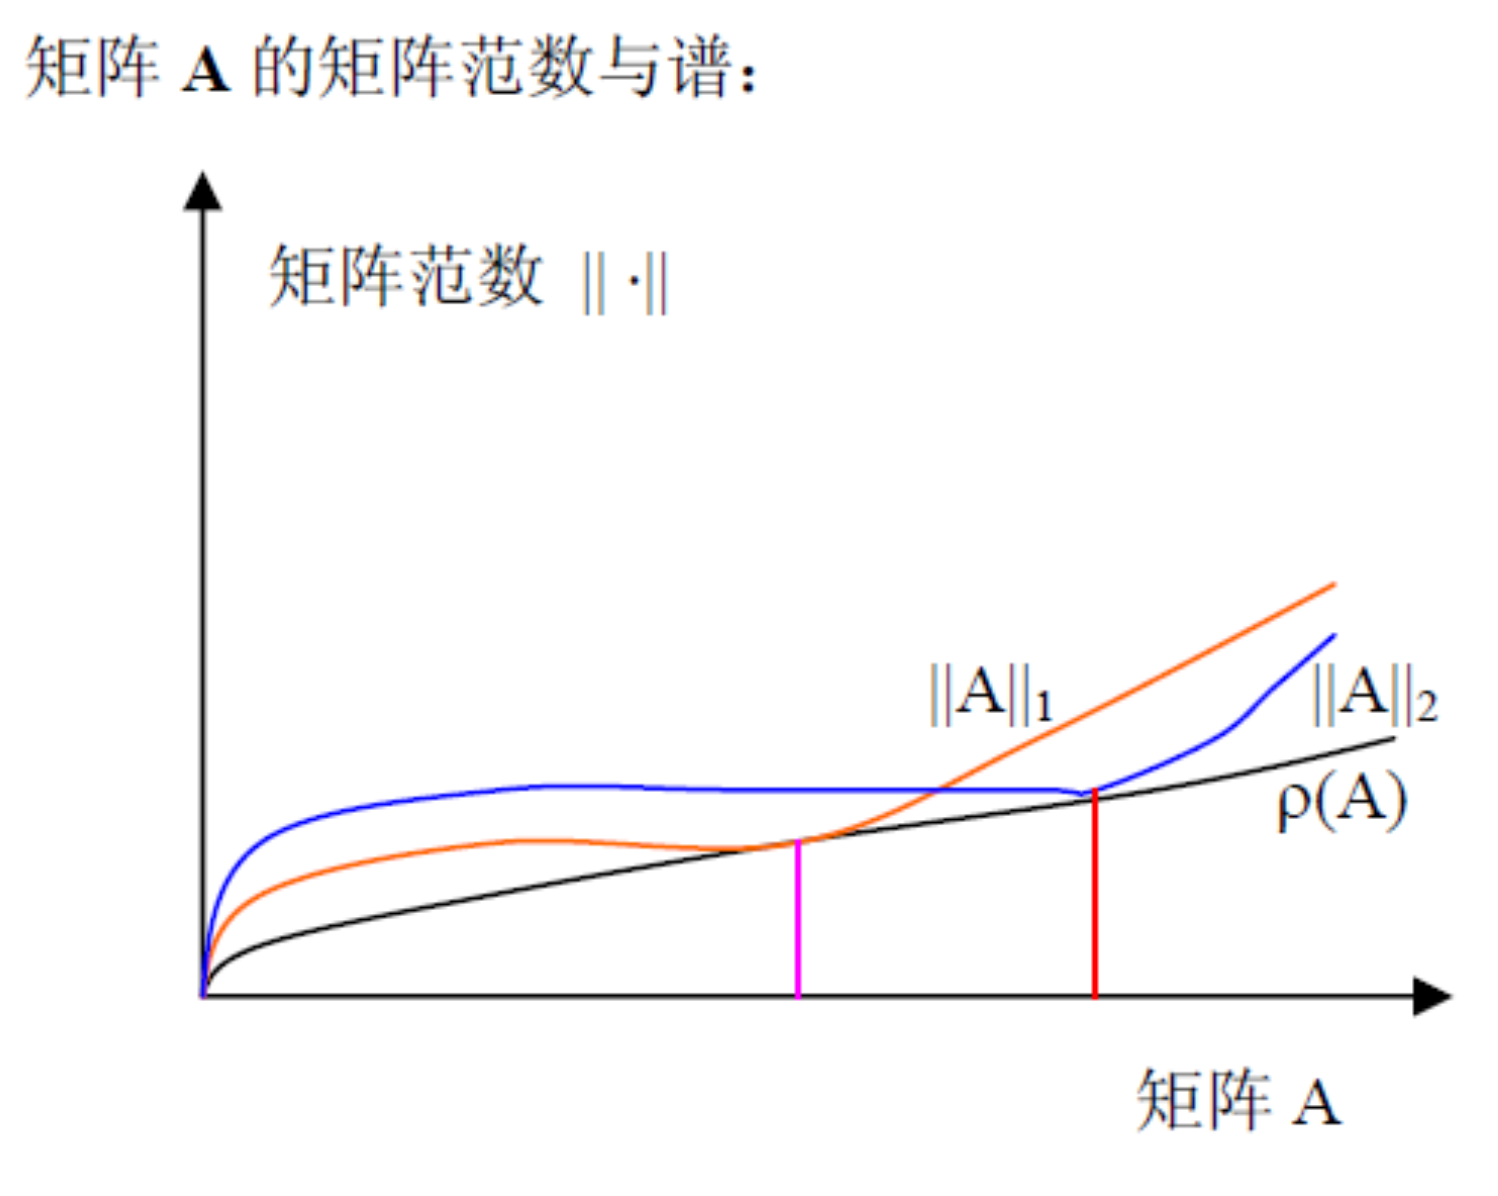
\includegraphics[width=0.4\linewidth]{figs/rho.png}
\end{figure}
\end{remark}
 \newpage
\section{矩阵分析及其应用}

\subsection{矩阵序列与矩阵级数}

\begin{definition}[矩阵序列的收敛]
设有矩阵序列 $\{A^{(k)}=(a_{ij}^{(k)})\}$，若各分量分别收敛，则称 $\{A^{(k)}\}$ 收敛；否则，若存在一组 $i,j$ 使得 $a_{ij}^{(k)}$ 发散，则称 $\{A^{(k)}\}$ 发散。
\end{definition}

\begin{theorem}[各分量收敛等价于依范数收敛]
设 $A^{(k)}\in\mathbb C^{m\times n}$，$\norm{\cdot}$ 为任一\textbf{广义矩阵范数}，则：
\begin{align*}
    &A^{(k)}\to 0\iff \norm{A^{(k)}}\to 0\\
    &A^{(k)}\to A\iff \norm{A^{(k)}-A}\to 0
\end{align*}
\end{theorem}
\begin{proof}
根据广义矩阵范数的等价性定理，仅需对 $m_\infty$ 范数证明。由于：
\[
    a^{(k)}\to 0\wedge b^{(k)}\to 0\iff\max(a^{(k)},b^{(k)})\to0
\]
所以：
\[
    A^{(k)}\to 0\iff |a_{ij}^{(k)}|\to 0\iff\norm{A}_{m_\infty}=\max_{i,j}|a_{ij}^{(k)}|\to 0
\]
\end{proof}

\begin{remark}
按各元素收敛需要验证 $m\times n$ 个数列是否收敛，比较麻烦；而依范数收敛只需要验证 1 个数列是否收敛，更加方便。
\end{remark}

\begin{remark}
尽管上述定理对任意\textbf{广义矩阵范数}都成立，但在证明时我们通常会选取一个\textbf{矩阵范数}，这样可以用上\textbf{相容性条件}，使得很多证明与高等数学中证明数列收敛没有什么区别。
\end{remark}

\begin{definition}[Cauchy 收敛]
矩阵序列 $\{A^{(k)}\}$ 收敛的充要条件是：对任意 $\epsilon>0$，存在 $N(\epsilon)$，当 $k,l\geq N(\epsilon)$ 时，有：
\[
    \norm{A^{(k)}-A^{(l)}}<\epsilon
\]
其中 $\norm\cdot$ 为任一广义矩阵范数。
\end{definition}

\begin{remark}
站在更高的泛函分析的角度，由于所有有限维赋范空间都是完备的，所以 Cauchy 列必收敛。
\end{remark}

\begin{property}
若 $A^{(k)}\to A$，则 $\norm{A^{(k)}}\to\norm{A}$.
\end{property}
\begin{proof}
\[
    \left|\norm{A^{(k)}}-\norm{A}\right|\leq\norm{A^{(k)}-A}\to0\implies\norm{A^{(k)}}\to\norm{A}
\]
\end{proof}

\begin{property}
设 $A^{(k)}\to A,\,B^{(k)}\to B$，则：
\begin{gather*}
    \lim_{k\to\infty}\left(\alpha A^{(k)}+\beta B^{(k)}\right)=\alpha A+\beta B\\
    \lim_{k\to\infty}A^{(k)}B^{(k)}=AB
\end{gather*}
\end{property}
\begin{proof}
只考虑相容的矩阵范数。
\begin{align*}
    \norm{A^{(k)}B^{(k)}-AB}&=\norm{A^{(k)}B^{(k)}-AB^{(k)}+AB^{(k)}-AB}\\
    &\leq\norm{A^{(k)}B^{(k)}-AB^{(k)}}+\norm{AB^{(k)}-AB}\\
    &\leq\norm{A^{(k)}-A}\norm{B^{(k)}}+\norm{A}\norm{B^{(k)}-B}
\end{align*}
由于 $\norm{A^{(k)}-A}\to0,\,\norm{B^{(k)}}\to\norm B,\,\norm{B^{(k)}-B}\to0$，所以 $\norm{A^{(k)}B^{(k)}-AB}\to0$，故 $A^{(k)}B^{(k)}\to AB$.
\end{proof}

\begin{theorem}
$A^{(k)}\to A$ 的充要条件是对任意 $x$ 有 $A^{(k)}x\to Ax$，或者对任意 $x,y$ 有 $y^HA^{(k)}x\to y^HAx$.
\end{theorem}

\begin{theorem}
若 $A^{(k)}$ 和 $A$ 都为 Hermite 矩阵，那么 $A^{(k)}\to A$ 的充要条件是 $x^HA^{(k)}x=x^HAx,\forall x$.
\end{theorem}

\begin{corollary}[类比单调有界定理]
若 $A^{(k)}$ 为半正定 Hermite 矩阵且单调减少（即 $A^{(k)}-A^{(k+1)}$ 为半正定 Hermite 矩阵），那么 $A^{(k)}$ 有极限。
\end{corollary}

\begin{property}
设 $A^{(k)}\to A$，且 $A^{(k)}$ 和 $A$ 都可逆，则：
\[
    \lim_{k\to\infty}\left(A^{(k)}\right)^{-1}=A^{-1}
\]
\end{property}

\begin{definition}[有界]
如果存在常数 $M>0$，使得对所有 $k$ 都有：
\[
    |a_{ij}^{(k)}|<M
\]
或等价地：
\[
    \norm{A^{(k)}}<M^\ast
\]
则称矩阵序列 $\{A^{(k)}\}$ 为有界的。
\end{definition}

\begin{theorem}
有界矩阵序列 $\{A^{(k)}\}$ 一定有收敛的子列。
\end{theorem}

\begin{definition}[收敛矩阵]
设 $A$ 为方阵且 $A^k\to 0\,(k\to\infty)$，则称 $A$ 为收敛矩阵。
\end{definition}

\begin{theorem}[迭代法基本定理]
\label{thm:iterbase}
$A$ 是收敛矩阵的充要条件是 $\rho(A)<1$.
\end{theorem}
\begin{proof}
必要性：设 $\lambda,x$ 为 $A$ 的特征值和特征向量，$\lambda x=Ax$，则 $\lambda^kx=A^kx$.  两边取范数：
\[
    |\lambda|^k\norm{x}=\norm{A^kx}\leq\norm{A^k}\norm{x}	
\]
由于 $x\neq 0$，故 $|\lambda|^k\leq\norm{A^k}\to0\,(k\to\infty)$，于是 $|\lambda|<1$，故 $\rho(A)=\max_i|\lambda_i|<1$.

充分性：取 $\epsilon=(1-\rho(A))/2$，根据定理 \ref{thm:specrad-norm}，存在某种矩阵范数使得：
\[
    \norm{A}<\rho(A)+\epsilon<1
\]
故：
\[
    \norm{A^k}\leq\norm{A}^k<(\rho(A)+\epsilon)^k\to 0\quad(k\to\infty)
\]
从而 $A^k\to0$.
\end{proof}

\begin{theorem}
$A$ 是收敛矩阵的充要条件是存在某种矩阵范数满足 $\norm{A}<1$.
\end{theorem}
\begin{proof}
根据迭代法基本定理和谱半径与矩阵范数的关系易证。
\end{proof}

\begin{remark}
实际应用中不会去算 $\rho(A)$（解特征值很麻烦），而是计算 $\norm{A}$.
\end{remark}

\begin{example}
在\textbf{迭代法解线性方程组}中，设迭代格式为 $x_{n+1}=Ax_n+f$，则：
\begin{align*}
    x_{n}&=Ax_{n-1}+f\\
    &=A^2x_{n-2}+Af+f\\
    &=\cdots\\
    &=A^n x_0+(A^{n-1}+\cdots+A+I)f\\
    &=A^n x_0+(I-A^n)(I-A)^{-1}f\\
    &=A^nx_0+(I-A)^{-1}f-A^n(I-A)^{-1}f
\end{align*}
若迭代收敛，则解满足 $x=Ax+f\implies x=(I-A)^{-1}f$.  记 $\epsilon_n=x_n-x$ 表示第 $n$ 次迭代后的误差，$\epsilon_0=x_0-x$ 表示初始误差，那么：
\[
\epsilon_n=A^n\epsilon_0
\]
因此，当 $A$ 是收敛矩阵时，$\epsilon_n\to0$，迭代法收敛。
\end{example}

\begin{definition}[矩阵级数的收敛与绝对收敛]
称矩阵级数 $\sum_{k=0}^\infty A^{(k)}$ （绝对）收敛到 $S$，若其部分和序列 $\left\{S_N=\sum_{k=0}^N A^{(k)}\right\}$ （绝对）收敛，且极限为 $S$.
\end{definition}

\begin{property}
矩阵级数 $\sum_{k=0}^\infty A^{(k)}$ 收敛的充要条件是对任意向量 $x$，向量级数 $\sum_{k=0}^\infty A^{(k)}x$ 收敛。
\end{property}

\begin{property}
若矩阵级数是绝对收敛的，则它一定是收敛的，并且任意调换其项的顺序所得到的级数仍然是收敛的，且其和不变。
\end{property}

\begin{property}
矩阵级数 $\sum_{k=0}^\infty A^{(k)}$ 绝对收敛的充要条件是 $\sum_{k=0}^\infty\norm{A^{(k)}}$ 收敛。
\end{property}

\begin{property}
若矩阵级数 $\sum_{k=0}^\infty A^{(k)}$ （绝对）收敛，则 $\sum_{k=0}^\infty PA^{(k)}Q$ 也（绝对）收敛，且：
\[
    \sum_{k=0}^\infty PA^{(k)}Q=P\left(\sum_{k=0}^\infty A^{(k)}\right)Q
\]
\end{property}

\begin{property}
若两个矩阵级数都绝对收敛，且分别收敛到 $A,B$，则其 Cauchy 乘积 $\sum_{k=0}^\infty\sum_{i+j=k}A^{(i)}B^{(j)}$ 绝对收敛，且收敛到 $AB$.
\end{property}

\begin{theorem}
方阵 $A$ 的幂级数 $\sum_{k=0}^\infty A^k$ 收敛的充要条件是 $\rho(A)<1$，且收敛时的和为 $(I-A)^{-1}$.
\end{theorem}
\begin{proof}
必要性。由于级数 $I+A+A^2+\cdots$ 收敛，所以部分和序列 $S^{(k)}=I+A+\cdots+A^k$ 收敛。记 $T^{(k)}=I+A+\cdots+A^{k+1}$，则 $A^{k+1}=T^k-S^k\to0$，即 $A$ 是收敛矩阵。根据定理 \ref{thm:iterbase}，有 $\rho(A)<1$.

充分性。已知 $\rho(A)<1$，故 $A$ 为收敛矩阵，$A^k\to 0$.  于是 $S^{(k)}=I+A+\cdots+A^k=(I-A)^{-1}-(I-A)^{-1}A^{k+1}\to(I-A)^{-1}$.
\end{proof}

\begin{theorem}
若方阵 $A$ 的某一范数满足 $\norm{A}<1$，则部分和 $I+A+\cdots+A^N$ 与 $(I-A)^{-1}$ 之间的误差为：
\[
    \left\Vert(I-A)^{-1}-\sum_{k=0}^NA^k\right\Vert\leq\frac{\norm{A}^{N+1}}{1-\norm{A}}
\]
\end{theorem}
\begin{proof}
设 $B=(I-A)^{-1}-\sum_{k=0}^NA^k=(I-A)^{-1}A^{N+1}$，则 $(I-A)B=A^{N+1}$，即 $B=AB+A^{N+1}$，从而：
\[
    \norm{B}=\norm{AB+A^{N+1}}\leq\norm{A}\norm{B}+\norm{A}^{N+1}\implies\norm{B}\leq\frac{\norm{A}^{N+1}}{1-\norm{A}}
\]
\end{proof}

\begin{theorem}
设幂级数 $\sum_{k=0}^\infty c_kz^k$ 的收敛半径为 $r$，如果方阵 $A$ 满足 $\rho(A)<r$，则矩阵幂级数 $\sum_{k=0}^\infty c_kA^k$ 绝对收敛；若 $\rho(A)>r$，则矩阵幂级数发散。
\end{theorem}
\begin{proof}
根据定理 \ref{thm:specrad-norm}，存在某个矩阵范数 $\norm{A}$ 使得 $\rho(A)\leq\norm{A}<r$，于是：
\[
    \sum_{k=0}^{\infty}\norm{c_kA^k}=\sum_{k=0}^{\infty}|c_k|\norm{A^k}\leq\sum_{k=0}^\infty |c_k|\norm{A}^k
\]
右侧数项级数收敛，因此左侧收敛，即矩阵幂级数绝对收敛。

设 $A$ 的特征值 $\lambda=\rho(A)$，$x$ 为对应特征向量，则：
\[
    \sum_{k=0}^\infty c_k(A^kx)=\sum_{k=0}^\infty c_k(\lambda^k x)=\left(\sum_{k=0}^\infty c_k\lambda^k\right)x
\]
当 $\rho(A)>r$ 时，幂级数 $\sum_{k=0}^\infty c_k\lambda^k$ 发散，因此矩阵幂级数发散；反之同理。
\end{proof}


\subsection{矩阵函数}
\label{sec:3-matrix-function}

\begin{definition}[矩阵函数]
设一元函数 $f(z)$ 能展开为 $z$ 的幂级数：
\[
    f(z)=\sum_{k=0}^\infty c_kz^k,\quad |z|<r
\]
则当 $n$ 阶方阵 $A$ 满足 $\rho(A)<r$ 时，矩阵级数 $\sum_{k=0}^\infty c_kA^k$ 收敛，其和称为矩阵函数，记作：
\[
    f(A)=\sum_{k=0}^\infty c_k A^k
\]
\end{definition}

\begin{theorem}[代入规则]
若 $f(z)$ 能展开为 $z$ 的幂级数且 $f(z)=g(z)$ 对 $|z|<r$ 成立，则当 $\rho(A)<r$ 时，$f(A)=g(A)$.
\end{theorem}

\begin{theorem}[二元函数的代入规则]
若 $f(x,y)$ 能展开为 $x,y$ 的幂级数且 $f(x,y)=g(x,y)$，并且 $AB=BA$，则 $f(A,B)=g(A,B)$.
\end{theorem}

\begin{remark}
为什么要求 $AB=BA$？因为 $f(x,y)=\sum_{i=0}^\infty\sum_{j=0}^\infty c_{ij}x^iy^j$，中间项要求交换律才能合并。
\end{remark}

\begin{example}
\begin{gather*}
    \sin(A)=A-\frac{A^3}{3!}+\frac{A^5}{5!}-\cdots\\
    \cos(A)=I-\frac{A^2}{2!}+\frac{A^4}{4!}-\cdots\\
    e^A=I+A+\frac{A^2}{2!}+\frac{A^3}{3!}+\cdots
\end{gather*}
\end{example}

下面介绍矩阵函数的几种求法，包括待定系数法、数项级数求和法、对角形法和 Jordan 标准形法。

\paragraph{待定系数法}

给定 $A$，确定首一零化多项式 $g(\lambda)$，使得 $g(A)=0$，例如特征多项式或最小多项式均可。设：
\[
f(\lambda)=g(\lambda)q(\lambda)+r(\lambda)
\]
其中 $\deg r(\lambda)<\deg g(\lambda)$. 那么只要确定了 $r(\lambda)$，就有 $f(A)=r(A)$.

所以问题的关键在于如何确定 $r(\lambda)$. 我们并不需要解 $q(\lambda)$，只需要找 $\deg r(\lambda)$ 个函数值或导数值（$k$ 重根就求 $k-1$ 阶导）形成线性方程组，就能解系数方程（其实就是带有导数约束的插值问题）。具体而言，设 $g(\lambda)$ 的互异零点为 $\lambda_1,\ldots,\lambda_s$，对应重数为 $r_1,\ldots,r_s$，那么易知：
\[
    g^{(l)}(\lambda_i)=0,\quad l=0,\ldots,r_i-1;\,i=1,\ldots,s
\]
因此：
\[
    r^{(l)}(\lambda_i)=f^{(l)}(\lambda_i),\quad l=0,\ldots,r_i-1;\,i=1,\ldots,s
\]
解该方程组即可确定 $r(\lambda)$.

对于规模较小的问题，直接求解方程组即可。

\begin{example}
设 $A=\begin{bmatrix}2&0&0\\1&1&1\\1&-1&3\end{bmatrix}$，求 $e^A$.

解：特征方程为：
\[
\varphi(\lambda)=\begin{vmatrix}\lambda-2&0&0\\-1&\lambda-1&-1\\-1&1&\lambda-3\end{vmatrix}=(\lambda-2)^3
\]
设 $f(\lambda)=e^\lambda=\varphi(\lambda)q(\lambda)+r(\lambda)$，其中 $r(\lambda)=a\lambda^2+b\lambda+c$，则：
\[
    \begin{cases}
    r(2)=f(2)=e^2\\
    r'(2)=f'(2)=e^2\\
    r''(2)=f''(2)=e^2
    \end{cases}\implies
    \begin{cases}
    4a+2b+c=e^2\\
    4a+b=e^2\\
    2a=e^2
    \end{cases}\implies
    \begin{cases}
    a=e^2/2\\
    b=-e^2\\
    c=e^2
    \end{cases}
\]
故 $r(\lambda)=e^2/2\cdot(\lambda^2-2\lambda+2)$，故：
\[
    f(A)=r(A)=\frac{e^2}{2}(A^2-2A+2I)=\begin{bmatrix}\cdots\end{bmatrix}
\]
\end{example}

对于规模较大的问题，可以考虑 Sylvester 插值公式或广义 Newton 插值公式。

\paragraph{Sylvester 插值公式} 暂略。

\paragraph{广义 Newton 插值公式}

正如上文所说，解方程组的本质就是解带有导数约束的插值问题。我们知道 Taylor 展开式满足在\textbf{一个点}处的 $n$ 阶\textbf{导数值}相等，而 Newton 展开式满足在\textbf{多个点}处的\textbf{函数值}相等，所以我们想解决的插值问题其实是二者的结合，遂称作广义 Newton 插值。

首先看 Taylor 展开式。若已知 $f(x)$ 在 $x_0$ 的函数值和直到 $n$ 阶导数值，则：
\[
    Tf(x)=f(x_0)+f'(x_0)(x-x_0)+\frac{f''(x_0)}{2!}(x-x_0)^2+\cdots+\frac{f^{(n)}(x_0)}{n!}(x-x_0)^n
\]
使得 $Tf^{(l)}(x_0)=f^{(l)}(x_0),\,l=0,\ldots,n$ 成立。

然后看 Newton 展开式。若已知 $f(x)$ 在互异点 $x_0,x_1,\ldots,x_n$ 处的函数值，则有 Newton 插值公式：
\begin{align*}
    Nf(x)&=f(x_0)\\
    &+f[x_0,x_1](x-x_0)\\
    &+f[x_0,x_1,x_2](x-x_0)(x-x_1)\\
    &+\cdots\\
    &+f[x_0,x_1,\ldots,x_n](x-x_0)(x-x_1)\cdots(x-x_{n-1})
\end{align*}
使得 $Nf(x_i)=f(x_i),\,i=0,\ldots,n$ 成立。
其中 $f[x_0,x_1]$ 称作一阶均差：
\[
    f[x_0,x_1]=\frac{f(x_1)-f(x_0)}{x_1-x_0}
\]
$f[x_0,x_1,x_2]$ 称作二阶均差：
\[
    f[x_0,x_1,x_2]=\frac{f[x_1,x_2]-f[x_0,x_1]}{x_2-x_0}
\]
$f[x_0,x_1,\ldots,x_k]$ 称作 $k$ 阶均差：
\[
    f[x_0,x_1,\ldots,x_k]=\frac{f[x_1,\ldots,x_{k-1},x_k]-f[x_0,x_1,\ldots,x_{k-1}]}{x_k-x_0}
\]
可以借助下面这个三角形表格来计算均差：
\begin{figure}[H]
    \centering
    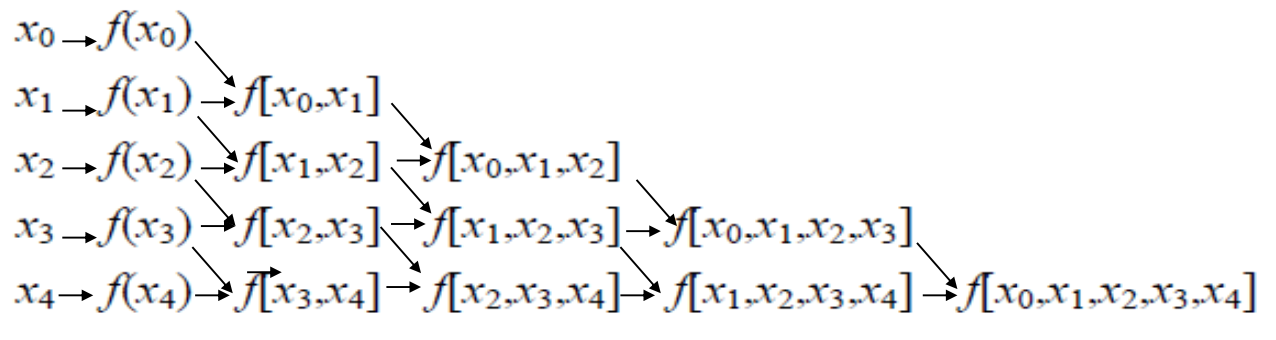
\includegraphics[width=0.7\linewidth]{figs/diff.png}
\end{figure}

将 Taylor 展开式和 Newton 展开式进行推广，可以得到广义 Newton 展开式。从均差的定义可以看出，它的极限与导数有密切关系。事实上，利用罗尔定理可以证明：若 $f(x)$ 在 $[a,b]$ 上存在 $n$ 阶导数，且节点 $x_0,x_1,\ldots,x_n\in[a,b]$，则存在 $\xi\in[a,b]$ 使得：
\[
    f([x_0,x_1,\ldots,x_n])=\frac{f^{(n)}(\xi)}{n!}
\]
因此，我们可以定义在相同点处的“广义”均差为：
\[
    f([c,c,\ldots,c])=\frac{f^{(n)}(c)}{n!}
\]
那么，Taylor 展开就可以看作是广义 Newton 展开在插值节点重合的特殊情形。
广义的均差也可以借助均差表计算，例如：
\begin{figure}[H]
    \centering
    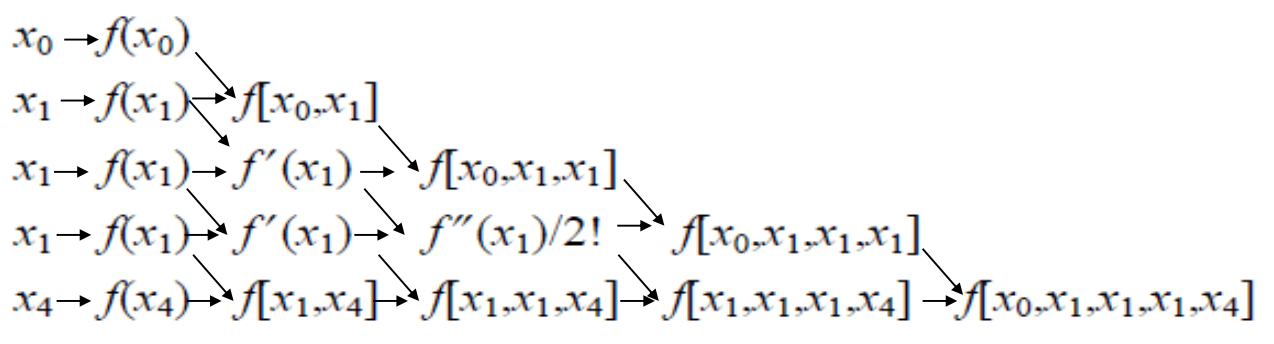
\includegraphics[width=0.7\linewidth]{figs/diff2.png}
\end{figure}

\begin{example}
设 $A=\begin{bmatrix}2&0&0\\1&1&2\\1&-1&3\end{bmatrix}$，求 $e^{At}$.

解：特征方程为：
\[
    \varphi(\lambda)=\begin{vmatrix}\lambda-2&0&0\\-1&\lambda-1&-2\\-1&1&\lambda-3\end{vmatrix}=(\lambda-2)(\lambda-5)(\lambda+1)
\]
画均差表：
\begin{figure}[H]
    \centering
    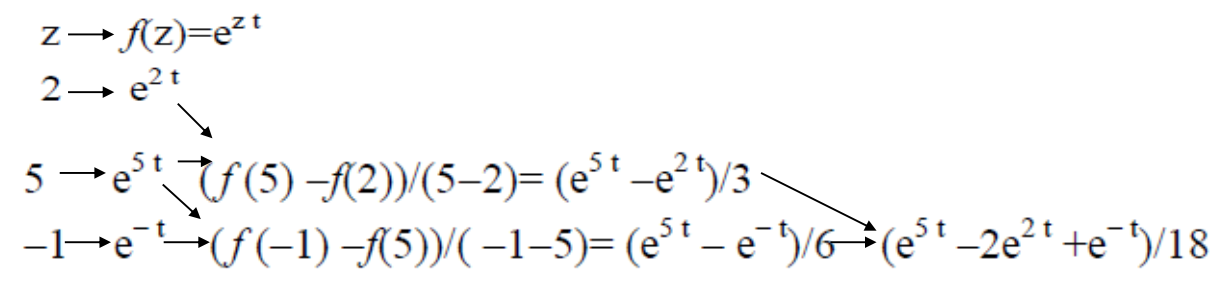
\includegraphics[width=0.7\linewidth]{figs/diff-ex.png}
\end{figure}
于是：
\[
    r(\lambda)=e^{2t}+\frac{e^{5t}-e^{2t}}{3}(\lambda-2)+\frac{e^{5t}-2e^{2t}+e^{-t}}{18}(\lambda-2)(\lambda-5)
\]
故：
\[
    e^{At}=r(A)=\cdots
\]
\end{example}

\paragraph{数项级数求和法}

暂略。



\paragraph{对角形法}

若 $A$ 可对角化，即存在非奇异矩阵 $P$，使得：
\[
    P^{-1}AP=\begin{bmatrix}\lambda_1&&\\&\ddots&\\&&\lambda_n\end{bmatrix}
\]
则：
\[
    f(A)=P\begin{bmatrix}f(\lambda_1)&&\\&\ddots&\\&&f(\lambda_n)\end{bmatrix}P^{-1}
\]

\begin{note}
对角化的计算量较大，因为要计算 $P$ 和 $P^{-1}$，即解特征值和特征向量。
\end{note}


\paragraph{Jordan 标准形法}

在第一章中我们已经推导过了 Jordan 标准形的多项式，而对于一般函数，根据代入规则容易知道其结论有类似的形式。

设 $A$ 的 Jordan 标准形为 $J$，则存在可逆矩阵 $P$ 使得：
\[
    P^{-1}AP=J=\begin{bmatrix}J_1&&\\&\ddots&\\&&J_s\end{bmatrix},\quad J_i=\begin{bmatrix}\lambda_i&1&&\\&\ddots&\ddots&\\&&\lambda_i&1\\&&&\lambda_i\end{bmatrix}_{m_i\times m_i}
\]
那么：
\[
    f(J_i)=\begin{bmatrix}
    f(\lambda_i)&\frac{1}{1!}f'(\lambda_i)&\frac{1}{2!}f''(\lambda_i)&\cdots&\frac{1}{(m_i-1)!}f^{(m_i-1)}(\lambda_i)\\
    &f(\lambda_i)&\frac{1}{1!}f'(\lambda_i)&\cdots&\frac{1}{(m_i-2)!}f^{(m_i-2)}(\lambda_i)\\
    &&\ddots&\ddots&\vdots\\
    &&&f(\lambda_i)&\frac{1}{1!}f'(\lambda_i)\\
    &&&&f(\lambda_i)
    \end{bmatrix}_{m_i\times m_i}
\]
于是原问题：
\[
    f(A)=Pf(J)P^{-1}=P\begin{bmatrix}f(J_1)&&\\&\ddots&\\&&f(J_s)\end{bmatrix}P^{-1}
\]


\subsection{矩阵的微分与积分}

\begin{definition}[矩阵的导数]
若 $A(t)=\left(a_{ij}(t)\right)\in\mathbb C^{m\times n}$ 的每个元素 $a_{ij}(t)$ 都是 $t$ 的可微函数，则 $A(t)$ 关于 $t$ 的导数定义为：
\[
    \frac{\mathrm d}{\mathrm dt}A(t)=A'(t)=\left(a'_{ij}(t)\right)_{m\times n}
\]
\end{definition}
\begin{property}
\[
    \frac{\mathrm d}{\mathrm dt}(A(t)+B(t))=\frac{\mathrm d}{\mathrm dt}A(t)+\frac{\mathrm d}{\mathrm dt}B(t)
\]
\end{property}
\begin{property}
\[
    \frac{\mathrm d}{\mathrm dt}(A(t)B(t))=\frac{\mathrm d}{\mathrm dt}A(t)\cdot B(t)+A(t)\cdot\frac{\mathrm d}{\mathrm dt}B(t)
\]
\end{property}
\begin{corollary}
若 $C(t)=A(t)B(t)$，则：
\[
    \mathrm dC=\mathrm dA\cdot B+A\cdot\mathrm dB
\]
其中，$\mathrm dA=(\mathrm dA/\mathrm dt)\cdot \mathrm dt$，$\mathrm dB=(\mathrm dB/\mathrm dt)\cdot \mathrm dt$.
\end{corollary}

\begin{example}[逆矩阵的导数]
\[
    \frac{\mathrm d}{\mathrm dt}\left(A(t)^{-1}\right)=-A(t)^{-1}\frac{\mathrm dA(t)}{\mathrm dt}A(t)^{-1}
\]
\end{example}
\begin{proof}
由于 $A(t)\cdot A(t)^{-1}=I$，两边求导得：
\[
    \frac{\mathrm d}{\mathrm dt}A(t)\cdot A(t)^{-1}+A(t)\cdot\frac{\mathrm d}{\mathrm dt}\left(A(t)^{-1}\right)=0
\]
故：
\[
    \frac{\mathrm d}{\mathrm dt}\left(A(t)^{-1}\right)=-A(t)^{-1}\frac{\mathrm dA(t)}{\mathrm dt}A(t)^{-1}
\]
\end{proof}

\begin{property}
\[
    \frac{\mathrm d}{\mathrm dt}(\alpha(t)A(t))=\alpha'(t)A(t)+\alpha(t)\cdot\frac{\mathrm d}{\mathrm dt}A(t)
\]
\end{property} 
\begin{property}
若 $A(t)$ 和 $\frac{\mathrm d}{\mathrm dt}A(t)$ \textbf{可交换}，$f(z)$ 是与 $t$ 无关的一元解析函数，则：
\[
    \frac{\mathrm d}{\mathrm dt}f(A(t))=f'(A(t))\cdot\frac{\mathrm d}{\mathrm dt}A(t)
\]
\end{property}
\begin{proof}[形式证明（不严格）]
若将 $f(z)$ 展开为幂级数的形式 $f(z)=\sum_{k=0}^\infty c_kz^k$，则根据可交换条件有：
\[
    \frac{\mathrm d}{\mathrm dt}A^k(t)=\sum_{i=0}^{k-1}A^i(t)\cdot\frac{\mathrm d}{\mathrm dt}A(t)\cdot A^{k-1-i}(t)=kA^{k-1}(t)\cdot\frac{\mathrm d}{\mathrm dt}A(t)
\]
代入矩阵函数得：
\[
    \frac{\mathrm d}{\mathrm dt}f(A(t))=\sum_{k=0}^\infty c_k\left(kA^{k-1}(t)\cdot\frac{\mathrm d}{\mathrm dt}A(t)\right)=f'(A(t))\cdot\frac{\mathrm d}{\mathrm dt}A(t)
\]
\end{proof}

\begin{property}[迹函数求导基本定理]
若 $A(t)$ 和 $B(t)$ 可交换，$f(z)$ 是与 $t$ 无关的一元解析函数，则：
\[
    \frac{\mathrm d}{\mathrm dt}\mathrm{tr}\big(f(A(t))\cdot B(t)\big)=\mathrm{tr}\left(f'(A(t))\cdot\frac{\mathrm d}{\mathrm dt}A(t)B(t)\right)+\mathrm{tr}\left(f(A(t))\cdot\frac{\mathrm d}{\mathrm dt}B(t)\right)
\]
\end{property}
\begin{corollary}
取 $B(t)=I$，则有：
\[
    \frac{\mathrm d}{\mathrm dt}\mathrm{tr}(f(A(t)))=\mathrm{tr}\left(f'(A(t))\cdot\frac{\mathrm d}{\mathrm dt}A(t)\right)
\]
\end{corollary}

\begin{definition}[矩阵的积分]
若矩阵 $A(t)=(a_{ij}(t))\in\mathbb C^{m\times n}$ 的每个元素 $a_{ij}(t)$ 都在 $[t_0,t]$ 上可积，则称 $A(t)$ 可积，记为：
\[
    \int_{t_0}^t A(\tau)\mathrm d\tau=\left(\int_{t_0}^ta_{ij}(\tau)\mathrm d\tau\right)_{m\times n}
\]
\end{definition}
\begin{property}
\[
    \int_{t_0}^t[A(\tau)+B(\tau)]\mathrm d\tau=\int_{t_0}^tA(\tau)\mathrm d\tau+\int_{t_0}^tB(\tau)\mathrm d\tau
\]
\end{property}
\begin{property}
\begin{align*}
    &\int_{t_0}^t[A\cdot B(\tau)]\mathrm d\tau=A\cdot\left[\int_{t_0}^tB(\tau)\mathrm d\tau\right]\\
    &\int_{t_0}^t[A(\tau)\cdot B]\mathrm d\tau=\left[\int_{t_0}^tA(\tau)\mathrm d\tau\right]\cdot B
\end{align*}
\end{property}
\begin{property}
\[
    \frac{\mathrm d}{\mathrm dt}\int_{t_0}^tA(\tau)\mathrm d\tau=A(t)
\]
\end{property}
\begin{property}
\[
    \int_{t_0}^{t_1}A'(\tau)\mathrm d\tau=A(t_1)-A(t_0)
\]
\end{property}

\vskip 6pt

前文涉及到的矩阵函数是从矩阵到矩阵的映射，接下来我们探讨关于矩阵各个元素的函数，即从矩阵到数的映射，称作\textbf{函数矩阵}。注意区分函数矩阵与矩阵函数。
为了方便后续推导，首先列出\textbf{矩阵元素与矩阵符号的代数关系式}，可以帮助避免将矩阵的各个分量列出来的繁琐。
我们约定 $e_i$ 表示第 $i$ 个分量为 1、其余分量为 0 的单位列向量，其维数由上下文确定，即同一个式子中出现的 $e_i,e_j$ 可能是不同维数的。那么有以下关系式：

\begin{itemize}
    \item 用分量表示矩阵：
    \[
        A=\sum_{i=1}^m\sum_{j=1}^na_{ij}e_ie_j^T
    \]

    \item 用矩阵表示分量：
    \[
        a_{ij}=e_i^TAe_j
    \]

    \item 矩阵逐列拉成向量：
    \[
        \text{Vec}(A)=\sum_{i=1}^m\sum_{j=1}^na_{ij}e_j\otimes e_i=\sum_{i=1}^mA^T e_i\otimes e_i=\sum_{j=1}^ne_j\otimes Ae_j
    \]

    \item 用拉成向量的矩阵表示分量：
    \[
        a_{ij}=(e_j\otimes e_i)^T\text{Vec}(A)
    \]
\end{itemize}

\begin{definition}[函数矩阵的导数]
设 $X=(\xi_{ij})_{m\times n}$，$f(X)$ 为 $mn$ 元函数：
\[
    f(X)=f(\xi_{11},\ldots,\xi_{1n},\xi_{21},\ldots,\xi_{2n},\ldots,\xi_{m1},\ldots,\xi_{mn})
\]
定义 $f(X)$ 对矩阵 $X$ 的导数为：
\[
    \frac{\mathrm df}{\mathrm dX}=\left(\frac{\partial f}{\partial \xi_{ij}}\right)_{m\times n}=
    \begin{bmatrix}
    \dfrac{\partial f}{\partial \xi_{11}}&\cdots&\dfrac{\partial f}{\partial \xi_{1n}}\\
    \vdots&\ddots&\vdots\\
    \dfrac{\partial f}{\partial \xi_{m1}}&\cdots&\dfrac{\partial f}{\partial \xi_{mn}}\\
    \end{bmatrix}
    =\sum_{i=1}^m\sum_{j=1}^n\frac{\partial f}{\partial \xi_{ij}}e_ie_j^T
\]
\end{definition}

\begin{theorem}[函数矩阵的微分形式]
设 $X=(\xi_{ij})_{m\times n}$，$f(X)$ 为 $mn$ 元函数：
\[
    f(X)=f(\xi_{11},\ldots,\xi_{1n},\xi_{21},\ldots,\xi_{2n},\ldots,\xi_{m1},\ldots,\xi_{mn})
\]
则有：
\[
    \frac{\mathrm df}{\mathrm dX}=A\iff \mathrm df=\mathrm{tr}(A^T\cdot\mathrm dX)=\mathrm{tr}(A\cdot \mathrm dX^T)
\]
\end{theorem}
\begin{proof}
\begin{align*}
    \mathrm df&=\sum_{i=1}^m\sum_{j=1}^n\frac{\partial f}{\partial\xi_{ij}}\mathrm d\xi_{ij}\\
    &=\sum_{i=1}^m\sum_{j=1}^n\left(e_i^T\frac{\mathrm df}{\mathrm dX}e_j\right)\left(e_i^T\cdot \mathrm dX\cdot e_j\right)\\
    &=\sum_{i=1}^m\sum_{j=1}^ne_j^T\left(\frac{\mathrm df}{\mathrm dX}\right)^Te_ie_i^T\cdot\mathrm dX\cdot e_j\\
    &=\sum_{j=1}^ne_j^T\left(\frac{\mathrm df}{\mathrm dX}\right)^T\left(\sum_{i=1}^me_ie_i^T\right)\cdot\mathrm dX\cdot e_j\\
    &=\sum_{j=1}^ne_j^T\left(\frac{\mathrm df}{\mathrm dX}\right)^T\mathrm dX\cdot e_j\\
    &=\mathrm{tr}\left(\left(\frac{\mathrm df}{\mathrm dX}\right)^T\mathrm dX\right)\\
    &=\mathrm{tr}(A^T\cdot\mathrm dX)
\end{align*}
\end{proof}

\begin{remark}
上述定理非常重要！！！它告诉我们：\textbf{要求 $\mathrm df/\mathrm dX$，只需要将 $\mathrm df$ 写作形如 $\mathrm{tr}(A^T\mathrm dX)$ 的形式，那么 $A$ 就是结果}。以下所有内容都围绕这一点展开。
\end{remark}

\begin{property}[链式法则]
设 $f(x)$ 是向量 $x$ 的函数，$x$ 是标量 $t$ 的函数 $x=x(t)$，则：
\[
    \frac{\mathrm df}{\mathrm dt}=\frac{\mathrm dx^T}{\mathrm dt}\cdot\frac{\mathrm df}{\mathrm dx}
\]
\end{property}
\begin{property}[链式法则]
设 $f(X)$ 是 $m\times n$ 矩阵 $X$ 各元素的函数，而 $X$ 又是标量 $t$ 的函数，则：
\[
    \frac{\mathrm df}{\mathrm dt}=\mathrm{tr}\left(\frac{\mathrm dX^T}{\mathrm dt}\cdot\frac{\mathrm df}{\mathrm dX}\right)
\]
\end{property}
\begin{proof}
根据微分形式：
\[
    \mathrm df=\mathrm{tr}\left(\left(\frac{\mathrm df}{\mathrm dX}\right)^T\mathrm dX\right),\quad \mathrm dX=\frac{\mathrm dX}{\mathrm dt}\mathrm dt
\]
有：
\[
    \mathrm df=\mathrm{tr}\left(\left(\frac{\mathrm df}{\mathrm dX}\right)^T\frac{\mathrm dX}{\mathrm dt}\mathrm dt\right)=\mathrm{tr}\left(\left(\frac{\mathrm df}{\mathrm dX}\right)^T\frac{\mathrm dX}{\mathrm dt}\right)\mathrm dt=\mathrm{tr}\left(\frac{\mathrm dX^T}{\mathrm dt}\cdot\frac{\mathrm df}{\mathrm dX}\right)\mathrm dt
\]
\end{proof}

\begin{example}[迹函数的导数]
\begin{align*}
    &\frac{\mathrm d}{\mathrm dX}\mathrm{tr}(X^TA)=A\\
    &\frac{\mathrm d}{\mathrm dX}\mathrm{tr}(A^TX)=A\\
    &\frac{\mathrm d}{\mathrm dX}\mathrm{tr}(AX)=A^T
\end{align*}
\end{example}
\begin{proof}
微分是线性算子，可以放入 $\mathrm{tr}(\cdot)$，因此：
\[
    \mathrm d(\mathrm{tr}(X^TA))=\mathrm{tr}(\mathrm d(X^TA))=\mathrm{tr}(\mathrm dX^T A)=\mathrm{tr}(A^T\mathrm dX)
\]
根据微分形式，$\mathrm d(\mathrm{tr}(X^TA))/\mathrm dX=A$.  其他两式类似。证毕。
\end{proof}
\begin{example}
设 $X$ 为可逆矩阵，$f(X)=\mathrm{tr}(AX^{-1})$，则：
\[
    \frac{\mathrm d}{\mathrm dX}f(X)=-(X^{-1}AX^{-1})^T
\]
\end{example}
\begin{proof}
\[
    \mathrm df(X)=\mathrm{tr}(\mathrm d(AX^{-1}))=\mathrm{tr}(A\cdot\mathrm dX^{-1})
\]
由于 $XX^{-1}=I$，两边取微分得：$\mathrm dX\cdot X^{-1}+X\cdot\mathrm dX^{-1}=0$，故 $\mathrm dX^{-1}=-X^{-1}\cdot\mathrm dX\cdot X^{-1}$，因此：
\[
    \mathrm df(X)=\mathrm{tr}\left(A\cdot(-X^{-1}\mathrm dX X^{-1})\right)=\mathrm{tr}\left((-X^{-1}AX^{-1})\mathrm dX\right)
\]
根据微分形式，$\mathrm df(X)/\mathrm dX=(-X^{-1}AX^{-1})^T$.
\end{proof}

\begin{example}
设 $f(x)=x^TAx$，则：
\[
    \frac{\mathrm df}{\mathrm dx}=(A+A^T)x
\]
\end{example}
\begin{proof}
\begin{align*}
    \mathrm df&=\mathrm d(x^TAx)=\mathrm dx^TAx+x^TA\mathrm dx=x^T A^T\mathrm dx+x^TA\mathrm dx\\&=x^T(A^T+A)\mathrm dx=\mathrm{tr}\left(((A+A^T)x)^T\cdot\mathrm dx\right)
\end{align*}
根据微分形式，$\mathrm df/\mathrm dx=(A+A^T)x$.
\end{proof}

\begin{example}
更多迹函数求导结论：
\begin{figure}[H]
    \centering
    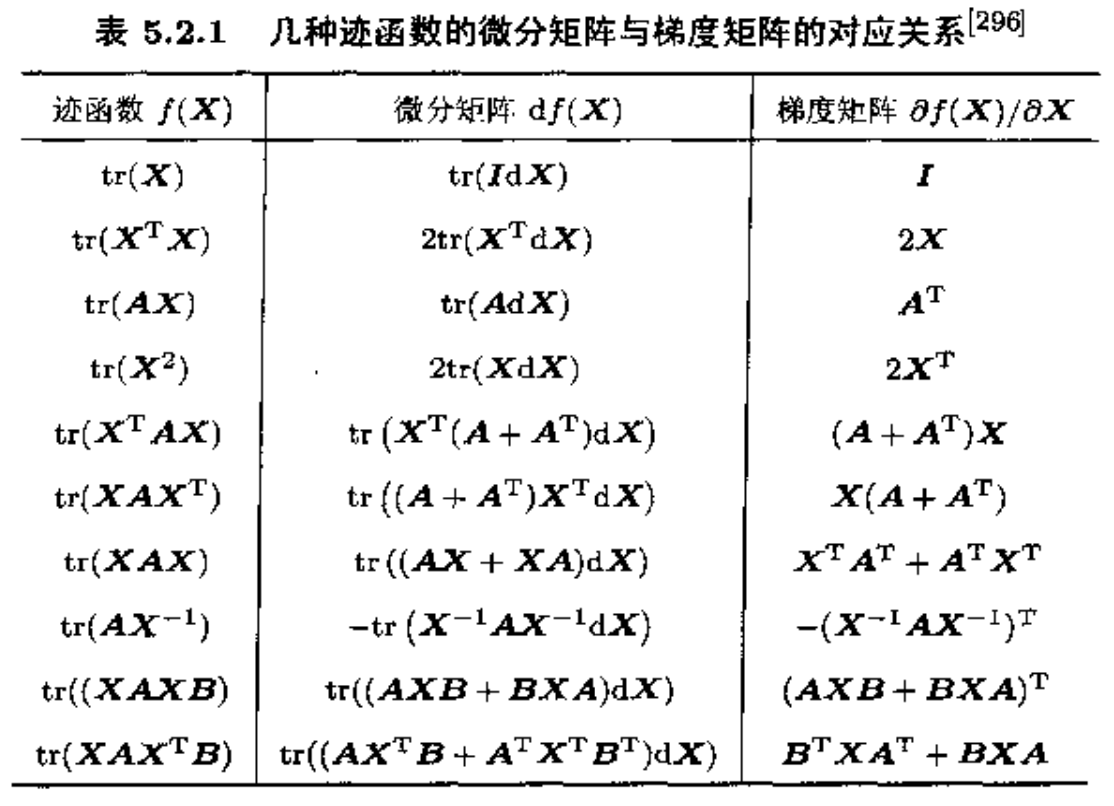
\includegraphics[width=0.7\linewidth]{figs/table1.png}
\end{figure}
\end{example}

\begin{example}[行列式求导]
设矩阵 $X$ 非奇异，则：
\[
    \frac{\mathrm d(|X|)}{\mathrm dX}=|X|(X^{-1})^T
\]
或有微分形式：
\[
    \mathrm d|X|=|X|\mathrm{tr}(X^{-1}\mathrm dX)=\mathrm{tr}(|X|X^{-1}\mathrm dX)
\]
\end{example}
\begin{proof}
设 $c_{ij}$ 为 $x_{ij}$ 的代数余子式，根据行列式定义知：
\[
    |X|=\sum_{i=1}^nc_{ij}x_{ij},\quad\forall j
\]
由于 $c_{ij}$ 与 $x_{ij}$ 无关，所以有 $\partial|X|/\partial x_{ij}=c_{ij}$，于是有微分：
\[
    \mathrm d|X|=\sum_{i=1}^n\sum_{j=1}^n c_{ij}\mathrm dx_{ij}=\mathrm{tr}(X^\ast\mathrm dX)
\]
其中 $X^\ast$ 是 $X$ 的伴随矩阵，由于 $X^\ast=|X|X^{-1}$，因此：
\[
    \mathrm d|X|=\mathrm{tr}(|X|X^{-1}\mathrm dX)
\]
\end{proof}

\begin{example}
对于任意非奇异矩阵 $X$，有：
\[
    \frac{\mathrm d(\ln|X|)}{\mathrm dX}=(X^T)^{-1}
\]
\end{example}
\begin{example}
对于任意 $X\in\mathbb R^{m\times n}$，
\[
    \frac{\mathrm d(\ln|\delta I+X^TX|)}{\mathrm dX}=2X(\delta I+X^TX)
\]
其中 $\delta$ 是与矩阵 $A$ 无关的常数。
\end{example}
\begin{example}
更多行列式求导结论：
\begin{figure}[H]
    \centering
    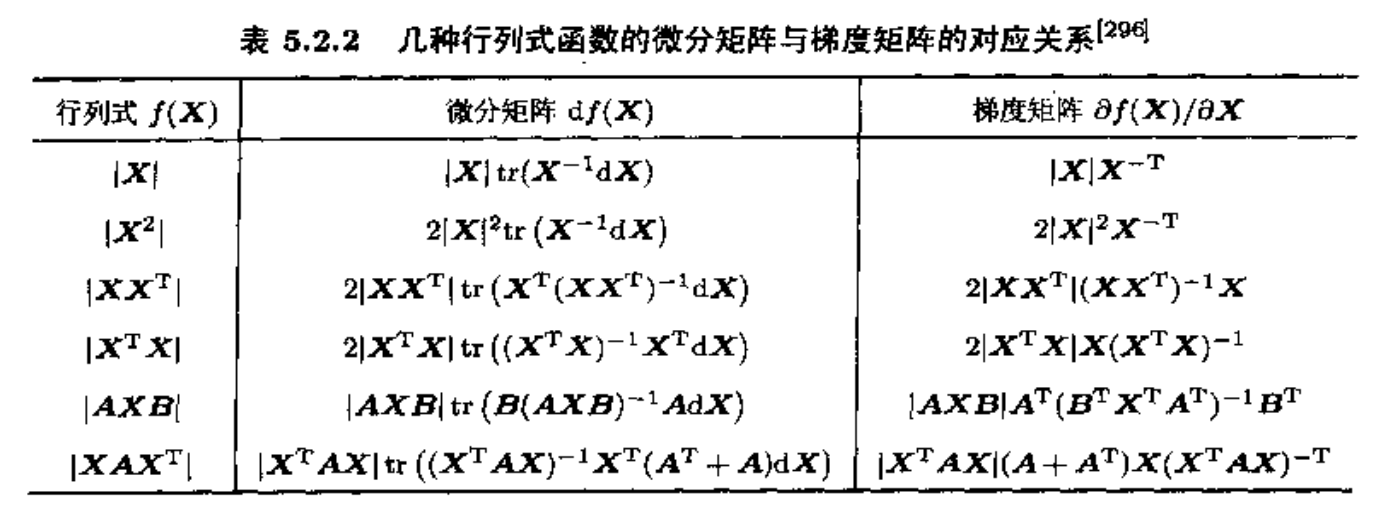
\includegraphics[width=0.9\linewidth]{figs/table2.png}
\end{figure}
\end{example}

\begin{definition}[直积 / Kronecker 积]
设 $A\in\mathbb C^{m\times n},\,B\in\mathbb C^{p\times q}$，称如下分块矩阵为 $A$ 与 $B$ 的直积：
\[
    A\otimes B=\begin{bmatrix}a_{11}B&a_{12}B&\cdots&a_{1n}B\\a_{21}B&a_{22}B&\cdots&a_{2n}B\\\vdots&\vdots&\ddots&\vdots\\a_{m1}B&a_{m2}B&\cdots&a_{mn}B\\\end{bmatrix}\in\mathbb C^{mp\times nq}
\]
特别地，若 $A\in\mathbb C^{m\times 1},\,B\in\mathbb C^{n\times 1}$，则 $A\otimes B^T=AB^T$.
\end{definition}

\begin{definition}[矩阵函数对矩阵的导数]
设有关于 $X=(\xi_{ij})_{m\times n}$ 的 $mn$ 元函数：
\[
    f_{ij}(X)=f_{ij}(\xi_{11},\ldots,\xi_{1n},\ldots,\xi_{m1},\ldots,\xi_{mn}),\quad i=1,\ldots,r,\,j=1,\ldots,s
\]
定义矩阵：
\[
    F(X)=\begin{bmatrix}f_{11}&\cdots&f_{1s}\\\vdots&\ddots&\vdots\\f_{r1}&\cdots&f_{rs}\end{bmatrix}
\]
定义 $F(X)$ 的导数如下：
\[
    \frac{\mathrm dF}{\mathrm dX}=
    \begin{bmatrix}
    \dfrac{\partial F}{\partial \xi_{11}}&\cdots&\dfrac{\partial F}{\partial \xi_{1n}}\\
    \vdots&\ddots&\vdots\\
    \dfrac{\partial F}{\partial \xi_{m1}}&\cdots&\dfrac{\partial F}{\partial \xi_{mn}}
    \end{bmatrix}=\sum_{i=1}^m\sum_{j=1}^n(e_ie_j^T)\otimes\frac{\partial F}{\partial \xi_{ij}}
\]
其中，
\[
    \frac{\partial F}{\partial \xi_{ij}}=
    \begin{bmatrix}
    \dfrac{\partial f_{11}}{\partial \xi_{ij}}&\cdots&\dfrac{\partial f_{1s}}{\partial \xi_{ij}}\\
    \vdots&\ddots&\vdots\\
    \dfrac{\partial f_{r1}}{\partial \xi_{ij}}&\cdots&\dfrac{\partial f_{rs}}{\partial \xi_{ij}}
    \end{bmatrix}=\sum_{k=1}^r\sum_{l=1}^s\frac{\partial f_{kl}}{\partial \xi_{ij}}e_ke_l^T
\]
特别地，当 $F\in\mathbb C^{m\times 1}$ 且 $X\in\mathbb C^{n\times 1}$ 时，
\[
    \frac{\mathrm dF}{\mathrm dX^T}=
    \begin{bmatrix}
    \dfrac{\partial f_{1}}{\partial \xi_{1}}&\cdots&\dfrac{\partial f_{1}}{\partial \xi_{n}}\\
    \vdots&\ddots&\vdots\\
    \dfrac{\partial f_{m}}{\partial \xi_{1}}&\cdots&\dfrac{\partial f_{m}}{\partial \xi_{n}}
    \end{bmatrix}
\]
即 Jacobian 矩阵。
\end{definition}

\begin{property}[链式法则]
设 $f(x)$ 是向量 $x$ 的函数，$x$ 又是 $u$ 的函数，则：
\[
    \frac{\mathrm df}{\mathrm du}=\frac{\mathrm dx^T}{\mathrm du}\frac{\mathrm df}{\mathrm dx}
\]
\end{property}

\begin{theorem}[向量函数关于向量导数的微分形式]
设 $y=F(x)$ 是向量 $x$ 的向量值函数，则：
\[
    \frac{\mathrm dy}{\mathrm dx^T}=A\iff\mathrm dy=A\mathrm dx
\]
\end{theorem}
\begin{note}
一些论文中可能会把 $\mathrm dy/\mathrm dx^T$ 不严谨地直接写作 $\mathrm dy/\mathrm dx$.
\end{note}

\begin{example}[在微分方程中的应用]
考虑微分方程：
\[
    \begin{cases}
    x_1'(t)=a_{11}x_1(t)+a_{12}x_2(t)+\cdots+a_{1n}x_n(t)+b_1(t)\\
    x_2'(t)=a_{21}x_1(t)+a_{22}x_2(t)+\cdots+a_{2n}x_n(t)+b_2(t)\\
    \quad\vdots\\
    x_n'(t)=a_{n1}x_1(t)+a_{n2}x_2(t)+\cdots+a_{nn}x_n(t)+b_n(t)\\
    \end{cases}
\]
令：
\[
    A=\begin{bmatrix}a_{11}&\cdots&a_{1n}\\\vdots&\ddots&\vdots\\a_{n1}&\cdots&a_{nn}\end{bmatrix},\quad
x(t)=\begin{bmatrix}x_1(t)\\\vdots\\x_n(t)\end{bmatrix},\quad
b(t)=\begin{bmatrix}b_1(t)\\\vdots\\b_n(t)\end{bmatrix}
\]
则可写作矩阵形式：
\[
    x'(t)=A\cdot x(t)+b(t)
\]
\end{example}

\begin{theorem}
齐次微分方程 $x'(t)=Ax(t)$ 的通解为：
\[
    x(t)=e^{tA}c
\]
其中 $c$ 为任意常向量。若再加上初始条件 $x(t_0)=x_0$，则解为：
\[
    x(t)=e^{(t-t_0)A}x_0
\]
\end{theorem}

\begin{theorem}
非齐次微分方程 $x'(t)=Ax(t)+b(t)$ 的通解为：
\[
    x(t)=x_1(t)+x_2(t)
\]
其中 $x_1(t)=e^{tA}c$ 是对应齐次微分方程的通解，$x_2(t)$ 是非齐次微分方程的一个特解。常向量 $c$ 由初始条件确定。特解可使用\textbf{常数变易法}计算得到：设 $x_2(t)=e^{tA}c(t)$，代入原非齐次微分方程有：
\[
    e^{tA}c'(t)=b(t)
\]
由此可以解出一个 $c(t)$，从而得到一个特解。
\end{theorem}
 \newpage
\section{矩阵分解}

\subsection{矩阵的三角分解}

矩阵的三角分解包括 LU 分解、LDU 分解、Doolittle 分解、Crout 分解和 Cholesky 分解等，其基本思想来自于\textbf{高斯消元法}。

\begin{definition}[初等矩阵]
初等行变换可以用左乘初等矩阵表示：
\begin{itemize}
    \item 交换两行：设 $u_{i,j}=(e_i-e_j)/\sqrt{2}$，
    \[
        I-2u_{i,j}u_{i,j}^T
    \]

    \item 第 $i$ 行乘以 $\alpha$ 加到第 $j$ 行：
    \[
        I+\alpha e_je_i^T
    \]

    \item 第 $i$ 行乘以 $\alpha$：
    \[
        I+(\alpha-1)e_ie_i^T
    \]
\end{itemize}
\end{definition}

\begin{definition}[消元因子]
第 $k$ 步消元时，若 $a_{kk}^{(k)}\neq 0$，则乘上消元因子 $m_{ik}=a_{ik}^{(k)}/a_{kk}^{(k)}$ 减到第 $i$ 行，其中 $i=k+1,\ldots,n$. 这相当于左乘矩阵： 
\[
    L_k=I-\left(\sum_{i=k+1}^nm_{ik}e_i\right)e_k^T=I-l_ke_k^T
\]
其中 $l_k=(0,\ldots,0,m_{k+1,k},m_{k+2,k},\ldots,m_{nk})^T$.
\end{definition}

\begin{theorem}
消元过程不改变矩阵的顺序主子式。
\end{theorem}

\begin{lemma}
约化的主元素 $a_{ii}^{(i)}\neq 0$ 的充要条件是矩阵 $A$ 的顺序主子式 $D_i\neq 0\,(i=1,\ldots,k)$.
\end{lemma}

\begin{corollary}
若矩阵 $A$ 的顺序主子式 $D_i\neq 0\,(i=1,\ldots,k)$，则：
\[
    a_{11}^{(1)}=D_1,\quad a_{ii}^{(i)}=D_i/D_{i-1}
\]
\end{corollary}

\begin{theorem}
若 $A$ 是正定矩阵，则一次消元后剩下的矩阵依旧是正定的。
\end{theorem}

\begin{theorem}
若 $A$ 严格对角占优，则一次消元后剩下的矩阵依旧是严格对角占优的。
\end{theorem}

\begin{definition}[LU 分解]
若方阵 $A$ 可以分解为一个下三角矩阵 $L$ 和一个上三角矩阵 $U$ 的乘积，即 $A=LU$，则称 $A$ 可作 LU 分解。
\end{definition}

\begin{com}
高斯消元的过程可以用 LU 分解表示：
\[
    \underbrace{L_{n-1}L_{n-2}\cdots L_2L_1}_{L^{-1}} A=U\implies A=LU
\]
其中 $L$ 为\textbf{单位}下三角矩阵，$U$ 为上三角矩阵。
\end{com}

\begin{definition}[LDU 分解]
若方阵 $A$ 可分解为 $A=LDU$，其中 $L$ 为\textbf{单位}下三角矩阵，$U$ 为\textbf{单位}上三角矩阵，$D$ 为对角矩阵，则称 $A$ 可作 LDU 分解。
\end{definition}

\begin{theorem}
设 $A$ 是 $n$ 阶方阵，当且仅当 $A$ 的顺序主子式 $\Delta_i\neq 0$ 时，$A$ 可唯一分解为 $A=LDU$，其中：
\[
    D=\text{diag}(d_1,\ldots,d_n),\quad d_k=\frac{\Delta_k}{\Delta_{k-1}}
\]
\end{theorem}

\begin{corollary}
$n$ 阶非奇异方阵 $A$ 有 LU 分解 $A=LU$ 的充要条件是顺序主子式 $\Delta_i\neq 0$.
\end{corollary}

\begin{theorem}
设 $A$ 是 $n$ 阶非奇异矩阵，则存在置换矩阵 $P$ 使得 $PA$ 的 $n$ 个顺序主子式非零。
\end{theorem}

\begin{corollary}[带有置换矩阵的三角分解]
设 $A$ 是 $n$ 阶非奇异方阵，则存在置换矩阵 $P$，使得：
\[
    PA=L\hat U=LDU
\]
其中 $L$ 为\textbf{单位}下三角矩阵，$\hat U$ 为上三角矩阵，$U$ 为\textbf{单位}上三角矩阵，$D$ 为对角矩阵。
\end{corollary}


\begin{definition}[Doolittle 分解]
把 LDU 分解中的 $DU$ 结合起来用 $\hat U$ 表示，得到唯一的分解：
\[
    A=L(DU)=L\hat U
\]
\end{definition}
\begin{definition}[Crout 分解]
把 LDU 分解中的 $LD$ 结合起来用 $\hat L$ 表示，得到唯一的分解：
\[
    A=(LD)U=\hat LU
\]
\end{definition}

\noindent\textbf{计算方法（以 Doolittle 分解为例）}：比较等式两边的元素逐行逐列求解 $L,U$ 各元素：
\[
    \begin{bmatrix}
    a_{11}&a_{12}&\cdots&a_{1n}\\
    a_{21}&a_{22}&\cdots&a_{2n}\\
    \vdots&\vdots&\ddots&\vdots\\
    a_{n1}&a_{n2}&\cdots&a_{nn}\\
    \end{bmatrix}=
    \begin{bmatrix}
    1&&&\\
    l_{21}&1&&\\
    \vdots&\vdots&\ddots&\\
    l_{n1}&l_{n2}&\cdots&1\\
    \end{bmatrix}
    \begin{bmatrix}
    u_{11}&u_{12}&\cdots&u_{1n}\\
    &u_{22}&\cdots&u_{2n}\\
    &&\ddots&\vdots\\
    &&&u_{nn}\\
    \end{bmatrix}
\]
\begin{figure}[H]
    \centering
    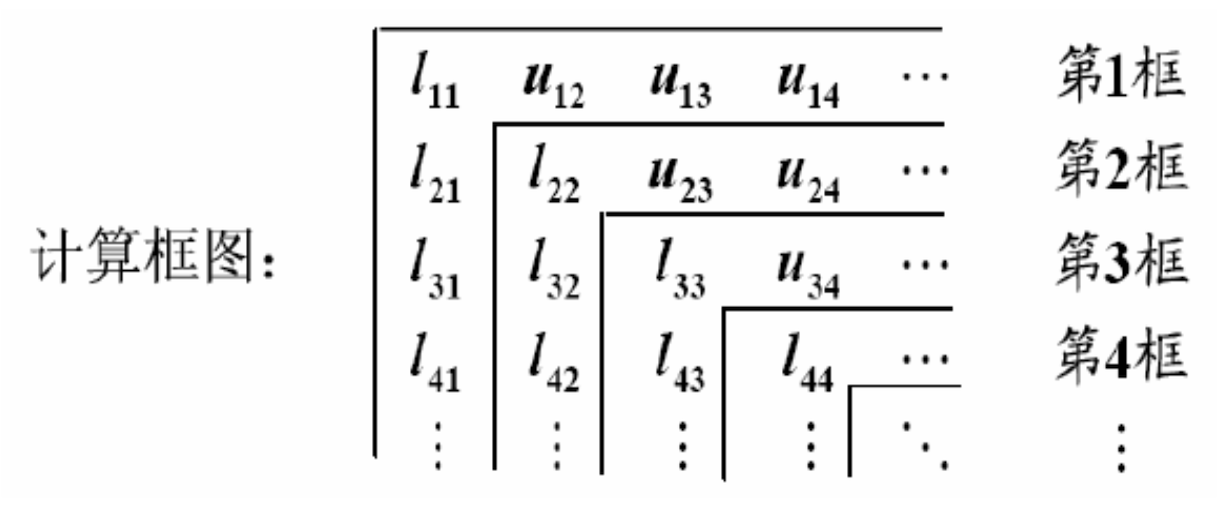
\includegraphics[width=0.5\linewidth]{figs/calc.png}
\end{figure}

\begin{definition}[Cholesky 分解]
若实对称正定矩阵可以按如下方式分解：
\[
    A=L\tilde D^2L^T\quad\text{或}\quad A=LDL^T\quad\text{或}\quad A=LL^T
\]
则称 $A$ 可作 Cholesky 分解。其中第二种表示中，$D$ 的对角元都大于零；第三种表示中，$L$ 的对角元都大于零。
\end{definition}

\noindent\textbf{计算方法}：与 Doolittle 分解的计算类似，逐行逐列计算即可：
\[
    \begin{bmatrix}
    a_{11}&a_{12}&\cdots&a_{1n}\\
    a_{21}&a_{22}&\cdots&a_{2n}\\
    \vdots&\vdots&\ddots&\vdots\\
    a_{n1}&a_{n2}&\cdots&a_{nn}\\
    \end{bmatrix}=
    \begin{bmatrix}
    l_{11}&&&\\
    l_{21}&l_{22}&&\\
    \vdots&\vdots&\ddots&\\
    l_{n1}&l_{n2}&\cdots&l_{nn}\\
    \end{bmatrix}
    \begin{bmatrix}
    l_{11}&l_{12}&\cdots&l_{1n}\\
    &l_{22}&\cdots&l_{2n}\\
    &&\ddots&\vdots\\
    &&&l_{nn}\\
\end{bmatrix}
\]
可得：
\[
    l_{jj}=\left(a_{jj}-\sum_{k=1}^{j-1}l_{jk}^2\right)^{1/2},\quad l_{ij}=\left(a_{ij}-\sum_{k=1}^{j-1}l_{ik}l_{jk}\right)/l_{jj}
\]
该计算方法的缺点是有开方运算，在计算机中由于浮点误差可能出现根号下负数。

\vskip 10pt \noindent\textbf{改进的 Cholesky 分解计算方法}：所谓改进的 Cholesky 分解，其实就是指 $A=LDL^T$，其计算过程不涉及开方，因而有更好的数值稳定性：
\[
    \begin{bmatrix}
    a_{11}&a_{12}&\cdots&a_{1n}\\
    a_{21}&a_{22}&\cdots&a_{2n}\\
    \vdots&\vdots&\ddots&\vdots\\
    a_{n1}&a_{n2}&\cdots&a_{nn}\\
    \end{bmatrix}=
    \begin{bmatrix}
    1&&&\\
    l_{21}&1&&\\
    \vdots&\vdots&\ddots&\\
    l_{n1}&l_{n2}&\cdots&1\\
    \end{bmatrix}
    \begin{bmatrix}
    d_1&d_1l_{12}&\cdots&d_1l_{1n}\\
    &d_2&\cdots&d_2l_{2n}\\
    &&\ddots&\vdots\\
    &&&d_n\\
    \end{bmatrix}
\]
逐行逐列计算可得：
\[
    l_{ij}=\left(a_{ij}-\sum_{k=1}^{j-1}l_{ik}d_kl_{jk}\right)/d_j,\quad d_i=a_{ii}-\sum_{k=1}^{j-1}l_{ik}^2d_k
\]

\begin{definition}[分块矩阵的拟 LU 分解和拟 LDU 分解]
只考虑 2 阶的分块矩阵：
\[
    A=\begin{bmatrix}A_{11}&A_{12}\\A_{21}&A_{22}\end{bmatrix}
\]
若 $A_{11}$ 可逆，设：
\[
    L=\begin{bmatrix}I_{n_1}&0\\-A_{21}A_{11}^{-1}&I_{n_2}\end{bmatrix}
\]
则：
\[
    LA=\begin{bmatrix}A_{11}&A_{12}\\0&A_{22}-A_{21}A_{11}^{-1}A_{12}\end{bmatrix}
\]
若 $A_{22}$ 可逆，可右乘矩阵（作列变换）得到类似的结果。
\end{definition}

\begin{lemma}[求逆引理 / Woodbury 公式]
\[
    (A+BC)^{-1}=A^{-1}-A^{-1}B(I+CA^{-1}B)^{-1}CA^{-1}
\]
\end{lemma}
\begin{proof}
考虑方程 $(A+BC)x=b$，令 $y=Cx$，则：
\[
    \begin{bmatrix}A&B\\-C&0\end{bmatrix}\begin{bmatrix}x\\y\end{bmatrix}=\begin{bmatrix}b\\0\end{bmatrix}
\]
利用高斯消元法：
\begin{figure}[H]
    \centering
    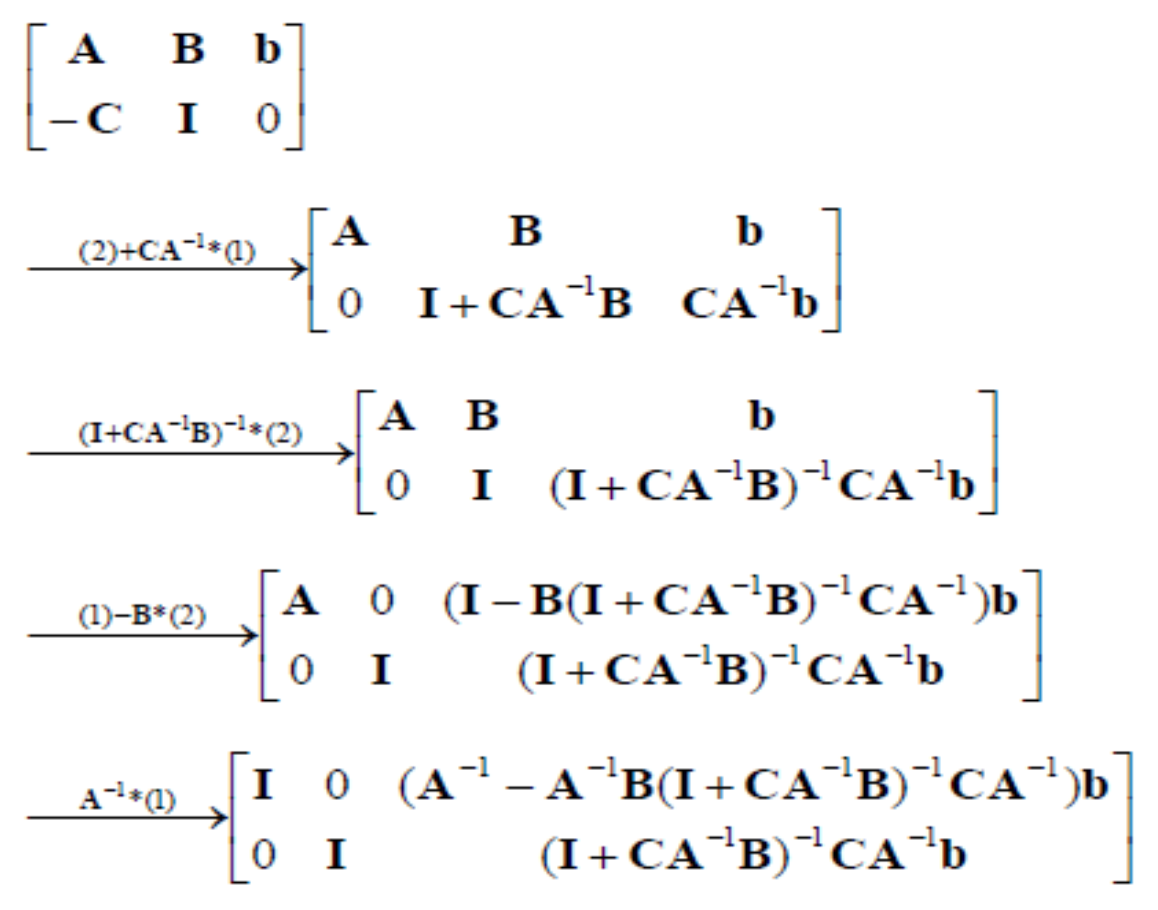
\includegraphics[width=0.5\linewidth]{figs/gauss.png}
\end{figure}
故解得：
\[
    x=(A^{-1}-A^{-1}B(I+CA^{-1}B)^{-1}CA^{-1})b
\]
又 $x=(A+BC)^{-1}b$，由 $b$ 的任意性可知命题成立。
\end{proof}

\begin{corollary}
\[
    (A+BD^{-1}C)^{-1}=A^{-1}-A^{-1}B(D+CA^{-1}B)^{-1}CA^{-1}
\]
\end{corollary}


\subsection{矩阵的 QR 分解}
\label{sec:qr}

\begin{definition}[Givens 矩阵，Givens 变换]
设 $c,s\in\mathbb R$ 且 $c^2+s^2=1$，称：
\[
    T_{ij}=T_{ij}(c,s)=
    \begin{bmatrix}
    1&      & &  & &      & & & &      & \\
     &\ddots& &  & &      & & & &      & \\
     &      &1&  & &      & & & &      & \\
     &      & &c & &      & &s& &      & \\
     &      & &  &1&      & & & &      & \\
     &      & &  & &\ddots& & & &      & \\
     &      & &  & &      &1& & &      & \\
     &      & &-s& &      & &c& &      & \\
     &      & &  & &      & & &1&      & \\
     &      & &  & &      & & & &\ddots& \\
     &      & &  & &      & & & &      &1\\
    \end{bmatrix}
\]
为 Givens 矩阵。由 Givens 矩阵确定的线性变换称作 Givens 变换（初等旋转变换）。
\end{definition}

\begin{remark}
顾名思义，Givens 变换的作用是旋转。具体而言，是在第 $i$ 和第 $j$ 维的平面上绕原点\textbf{顺时针}旋转 $\theta$，其中 $c=\cos\theta,\,s=\sin\theta$.
\end{remark}

\begin{property}
Givens 矩阵是正交矩阵，且有：
\[
    [T_{ij}(c,s)]^{-1}=[T_{ij}(c,s)]^T=T_{ij}(c,-s),\quad\det(T_{ij}(c,s))=1
\]
\end{property}

\begin{theorem}
设 $x=(\xi_1,\ldots,\xi_n)^T\neq0$，则存在有限个 Givens 矩阵的乘积，记作 $T$，使得 $Tx=|x|e_1$.
\end{theorem}
\begin{proof}[证明（构造性）]
构造 Givens 矩阵 $T_{12}(c,s)$：
\[
    c=\frac{\xi_1}{\sqrt{\xi_1^2+\xi_2^2}}\quad s=\frac{\xi_2}{\sqrt{\xi_1^2+\xi_2^2}}
\]
则：
\[
    T_{12}x=\left(\sqrt{\xi_1^2+\xi_2^2},0,\xi_3,\ldots,\xi_n\right)^T
\]
再对 $T_{12}x$ 构造 Givens 矩阵 $T_{13}(c,s)$：
\[
    c=\frac{\sqrt{\xi_1^2+\xi_2^2}}{\sqrt{\xi_1^2+\xi_2^2+\xi_3^2}}\quad s=\frac{\xi_3}{\sqrt{\xi_1^2+\xi_2^2+\xi_3^2}}
\]
则：
\[
    T_{13}(T_{12}x)=\left(\sqrt{\xi_1^2+\xi_2^2+\xi_3^2},0,0,\xi_4,\ldots,\xi_n\right)^T
\]
如此继续下去，最后对 $T_{1,n-1}\cdots T_{12}x$ 构造 Givens 矩阵 $T_{1n}(c,s)$：
\[
    c=\frac{\sqrt{\xi_1^2+\cdots\xi_{n-1}^2}}{\sqrt{\xi_1^2+\cdots\xi_{n-1}^2+\xi_n^2}}\quad s=\frac{\xi_n}{\sqrt{\xi_1^2+\cdots\xi_{n-1}^2+\xi_n^2}}
\]
则：
\[
    T_{1n}(T_{1,n-1}\cdots T_{12}x)=\left(\sqrt{\xi_1^2+\cdots\xi_n^2},0,\ldots,0\right)^T
\]
令 $T=T_{1n}T_{1,n-1}\cdots T_{12}$，则 $Tx=|x|e_1$.
\end{proof}
\begin{remark}
直观理解：依次把第 $2,3,\ldots,n$ 维转到 0 即可。
\end{remark}

\begin{corollary}
任给非零列向量 $x\in\mathbb R^n$ 及单位列向量 $z\in\mathbb R^n$，则存在有限个 Givens 矩阵的乘积，记作 $T$，使得 $Tx=|x|z$.
\end{corollary}

\noindent\textbf{快速 Givens 变换}：暂略。

\begin{definition}[Householder 矩阵，Householder 变换]
设 $u\in\mathbb R^n$ 是单位列向量，称：
\[
    H=I-2uu^T
\]
为 Householder 矩阵。由 Householder 矩阵确定的线性变换称作 Householder 变换（初等反射变换）。
\end{definition}

\begin{remark}
顾名思义，Householder 变换的作用是反射。具体而言，是对以 $u$ 为法向量的平面做反射。
\end{remark}

\begin{property}
Householder 矩阵对称、正交、对合、自逆，且行列式为 $-1$：
\[
    H^T=H,\quad H^TH=I,\quad H^2=I,\quad H^{-1}=H,\quad \det(H)=-1
\]
\end{property}

\begin{theorem}
任给非零列向量 $x\in\mathbb R^n$ 及单位列向量 $z\in\mathbb R^n$，则存在 Householder 矩阵 $H$，使得 $Hx=|x|z$.
\end{theorem}
\begin{proof}[证明（构造性）]
若 $x=|x|z$，取单位向量 $u$ 使得 $u\perp x$，则 $H_u=I-2uu^T$：
\[
    H_ux=(I-2uu^T)x=x-2uu^Tx=x=|x|z
\]
否则，$x\neq|x|z$，取 $u=\dfrac{x-|x|z}{\left|x-|x|z\right|}$，则：
\begin{align*}
H_ux&=\left[I-2\frac{(x-|x|z)(x-|x|z)^T}{|x-|x|z|^2}\right]x\\
&=x-\frac{2(x-|x|z)^Tx}{|x-|x|z|^2}(x-|x|z)\\
&=x-(x-|x|z)=|x|z
\end{align*}
\end{proof}
\begin{remark}
直观理解：找到 $x$ 和 $z$ 之间对称平面，取 $u$ 为该平面的单位法向量即可。
\end{remark}

\begin{theorem}
Givens 变换可写作两个 Householder 变换的乘积。
\end{theorem}
\begin{remark}
换句话说，一次旋转操作可以分解为两次反射操作。
\end{remark}
\begin{proof}
取
\begin{align*}
    &u=(0,\ldots,0,\sin(\theta/4),0,\ldots,0,\cos(\theta/4),0,\ldots,0)^T\\
    &v=(0,\ldots,0,\sin(3\theta/4),0,\ldots,0,\cos(3\theta/4),0,\ldots,0)^T
\end{align*}
可以验证 $T_{ij}=H_vH_u$.
\end{proof}
\begin{note}
Householder 矩阵并不能由若干个 Givens 矩阵的乘积表示，因为 $\det(H)=-1$ 而 $\det(G)=1$.
\end{note}

\begin{definition}[QR 分解]
\label{def:qr}
若实/复矩阵 $A$ 能分解成正交/酉矩阵 $Q$ 与\textbf{非奇异}上三角矩阵 $R$ 的乘积，即 $A=QR$，则称 $A$ 可作 QR 分解。
\end{definition}

\begin{theorem}[非奇异方阵的 QR 分解]
\label{thm:qr1}
对 $n$ 阶\textbf{非奇异}矩阵 $A$，QR 分解在除去相差一个对角元素的绝对值/模全等于 1 的对角矩阵外，分解唯一。
\end{theorem}
\begin{proof}[证明（实数情形）]
设 $A=Q_1R_1=Q_2R_2$，则 $P=Q_2^TQ_1=R_2R_1^{-1}$. 注意到 $P^TP=I$，所以 $P^T=P^{-1}$.  由于 $P$ 是上三角矩阵，所以 $P^{-1}$ 是上三角矩阵，$P^T$ 是下三角矩阵，二者又相等，因此只能是对角矩阵。又 $P^2=I$，所以对角元只能是 $\pm1$.  那么 $Q_1=Q_2P,\,R_1=PR_2$.
\end{proof}

\begin{theorem}[列满秩矩阵的 QR 分解]
\label{thm:qr2}
对 $m\times n$ 实/复矩阵 $A$，其 $n$ 列线性无关（即 $A$ 列满秩），则 $A$ 有分解 $A=QR$，其中 $Q$ 是 $m\times n$ 实/复矩阵，且 $Q^HQ=I$（即 $Q$ 是正交/酉矩阵的一部分），$R$ 是实/复非奇异上三角矩阵，且除去相差一个对角元素的绝对值/模全等于 1 的对角矩阵外，分解唯一。
\end{theorem}

\noindent\textbf{计算方法（基于 Gram-Schmidt 正交化过程）}：
设 $A=(a_1,\ldots,a_n)$ 非奇异，对其各列实施 Gram-Schmidt 正交化过程：
\[
    \begin{cases}
    b_1=a_1\\
    b_2=a_2-k_{21}b_1\\
    \quad\vdots\\
    b_n=a_n-k_{n,n-1}b_{n-1}-\cdots-k_{n1}b_1
    \end{cases}\implies
    \begin{cases}
    a_1=b_1\\
    a_2=b_2+k_{21}b_1\\
    \quad\vdots\\
    a_n=b_n+k_{n,n-1}b_{n-1}+\cdots+k_{n1}b_1
    \end{cases}
\]
写作矩阵形式：
\begin{align*}
    A=BK&\implies(a_1,a_2,\ldots,a_n)=(b_1,b_2,\ldots,b_n)\begin{bmatrix}1&k_{21}&\cdots&k_{n1}\\&1&\cdots&k_{n2}\\&&\ddots&\vdots\\&&&1\end{bmatrix}\\
    &\implies(a_1,a_2,\ldots,a_n)=\underbrace{\begin{bmatrix}\dfrac{b_1}{|b_1|},\dfrac{b_2}{|b_2|}\ldots,\dfrac{b_n}{|b_n|}\end{bmatrix}}_Q\underbrace{\begin{bmatrix}|b_1|&&&\\&|b_2|&&\\&&\ddots&\\&&&|b_n|\end{bmatrix}\begin{bmatrix}1&k_{21}&\cdots&k_{n1}\\&1&\cdots&k_{n2}\\&&\ddots&\vdots\\&&&1\end{bmatrix}}_R\\
    &\implies A=QR
\end{align*}
\begin{note}
基于 Gram-Schmidt 正交化过程的 QR 分解计算方法在高阶时容易出现数值不稳定，需要用下文的基于 Givens 变换或 Householder 变换的方法计算。
\end{note}

\noindent\textbf{计算方法（基于 Givens 变换）}：
任何 $n$ 阶\textbf{实非奇异}矩阵 $A$ 都可以通过左连乘 Givens 初等旋转矩阵化为上三角矩阵。
\begin{enumerate}
    \item 由于 $\det(A)\neq0$，因此 $A$ 的第一列 $(a_{11},a_{21},\ldots,a_{n1})^T\neq 0$，根据前文的定理，存在有限个 Givens 矩阵的乘积 $T_1$，使得
    \[
        T_1(a_{11},a_{21},\ldots,a_{n1})^T=\left|(a_{11},a_{21},\ldots,a_{n1})^T\right|\cdot e_1
    \]
    将 $T_1$ 作用在 $A$ 上得：
    \[
        T_1A=\left[\begin{array}{c:ccc}
        a_{11}^{(1)}&a_{12}^{(1)}&\cdots&a_{1n}^{(1)}\\
        \hdashline
        0&&&\\
        \vdots&&A^{(1)}&\\
        0&&&
        \end{array}\right]
    \]

    \item 由于 $\det(A^{(1)})\neq0$，因此 $A^{(1)}$ 的第一列 $\left(a_{22}^{(1)},a_{32}^{(1)},\ldots,a_{n2}^{(1)}\right)^T\neq0$，于是存在有限个 Givens 矩阵的乘积 $T_2$，使得
    \[
        T_2\left(a_{22}^{(1)},a_{32}^{(1)},\ldots,a_{n2}^{(1)}\right)^T=\left|\left(a_{22}^{(1)},a_{32}^{(1)},\ldots,a_{n2}^{(1)}\right)^T\right|\cdot e_1
    \]
    将 $T_2$ 作用在 $A$ 上得：
    \[
        T_2A^{(1)}=\left[\begin{array}{c:ccc}
        a_{22}^{(2)}&a_{23}^{(2)}&\cdots&a_{2n}^{(2)}\\
        \hdashline
        0&&&\\
        \vdots&&A^{(2)}&\\
        0&&&
        \end{array}\right]
    \]

    \item 重复上述步骤，直到第 $n-1$ 步：
    \[
        T_{n-1}A^{(n-2)}=\begin{bmatrix}a_{n-1,n-1}^{(n-1)}&a_{n-1,n}^{(n-1)}\\0&a_{nn}^{(n- 1)}\end{bmatrix}
    \]

    \item 最后，令：
    \[
        T=\begin{bmatrix}I_{n-2}&O\\O&T_{n-1}\end{bmatrix}\cdots\begin{bmatrix}I_{2}&O\\O&T_{3}\end{bmatrix}\begin{bmatrix}I_{1}&O\\O&T_{2}\end{bmatrix}T_1
    \]
    则：
    \[
        TA=\begin{bmatrix}
        a_{11}^{(1)}&a_{12}^{(1)}&\cdots&a_{1,n-1}^{(1)}&a_{1n}^{(1)}\\
        &a_{22}^{(2)}&\cdots&a_{2,n-1}^{(2)}&a_{2n}^{(2)}\\
        &&\ddots&\vdots&\vdots\\
        &&&a_{n-1,n-1}^{(n-1)}&a_{n-1,n}^{(n-1)}\\
        &&&&a_{nn}^{(n-1)}
        \end{bmatrix}
    \]
    即 $A=QR$，其中 $Q=T^{-1}=T^T$，$R$ 就是上面化出来的那一大坨上三角矩阵。
\end{enumerate}

\begin{remark}
该过程与高斯消元法有异曲同工之妙。
\end{remark}

\noindent\textbf{计算方法（基于 Householder 变换）}：任何 $n$ 阶\textbf{实非奇异}矩阵 $A$ 都可以通过左连乘 Householder 初等反射矩阵化为上三角矩阵。
\begin{enumerate}
    \item 由于 $\det(A)\neq0$，因此 $A$ 的第一列 $(a_{11},a_{21},\ldots,a_{n1})^T\neq 0$，根据前文的定理，存在一个 Householder 矩阵 $H_1$，使得
    \[
        H_1(a_{11},a_{21},\ldots,a_{n1})^T=\left|(a_{11},a_{21},\ldots,a_{n1})^T\right|\cdot e_1
    \]
    将 $H_1$ 作用在 $A$ 上得：
    \[
        H_1A=\left[\begin{array}{c:ccc}
        a_{11}^{(1)}&a_{12}^{(1)}&\cdots&a_{1n}^{(1)}\\
        \hdashline
        0&&&\\
        \vdots&&A^{(1)}&\\
        0&&&
        \end{array}\right]
    \]
    
    \item 由于 $\det(A^{(1)})\neq0$，因此 $A^{(1)}$ 的第一列 $\left(a_{22}^{(1)},a_{32}^{(1)},\ldots,a_{n2}^{(1)}\right)^T\neq0$，于是存在一个 Householder 矩阵 $H_2$，使得
    \[
        H_2\left(a_{22}^{(1)},a_{32}^{(1)},\ldots,a_{n2}^{(1)}\right)^T=\left|\left(a_{22}^{(1)},a_{32}^{(1)},\ldots,a_{n2}^{(1)}\right)^T\right|\cdot e_1
    \]
    将 $H_2$ 作用在 $A$ 上得：
    \[
        H_2A^{(1)}=\left[\begin{array}{c:ccc}
        a_{22}^{(2)}&a_{23}^{(2)}&\cdots&a_{2n}^{(2)}\\
        \hdashline
        0&&&\\
        \vdots&&A^{(2)}&\\
        0&&&
        \end{array}\right]
    \]
   
    \item 重复上述步骤，直到第 $n-1$ 步：
    \[
        H_{n-1}A^{(n-2)}=\begin{bmatrix}a_{n-1,n-1}^{(n-1)}&a_{n-1,n}^{(n-1)}\\0&a_{nn}^{(n-1)}\end{bmatrix}
    \]

    \item 最后，令：
    \[
        H=\begin{bmatrix}I_{n-2}&O\\O&H_{n-1}\end{bmatrix}\cdots\begin{bmatrix}I_{2}&O\\O&H_{3}\end{bmatrix}\begin{bmatrix}I_{1}&O\\O&H_{2}\end{bmatrix}H_1
    \]
    则：
    \[
        HA=\begin{bmatrix}
        a_{11}^{(1)}&a_{12}^{(1)}&\cdots&a_{1,n-1}^{(1)}&a_{1n}^{(1)}\\
        &a_{22}^{(2)}&\cdots&a_{2,n-1}^{(2)}&a_{2n}^{(2)}\\
        &&\ddots&\vdots&\vdots\\
        &&&a_{n-1,n-1}^{(n-1)}&a_{n-1,n}^{(n-1)}\\
        &&&&a_{nn}^{(n-1)}
        \end{bmatrix}
    \]
    即 $A=QR$，其中 $Q=H^{-1}=H^T$，$R$ 就是上面化出来的那一大坨上三角矩阵。
\end{enumerate}

% ## Hessenberg 矩阵的正交相似

\begin{definition}[Hessenberg 矩阵]
称次对角线以下全为零的矩阵为 Hessenberg 矩阵。
\[
    F=\begin{bmatrix}
    a_{11}&a_{12}&a_{13}&\cdots&a_{1,n-1}&a_{1n}\\
    a_{21}&a_{22}&a_{23}&\cdots&a_{2,n-1}&a_{2n}\\
    0&a_{32}&a_{33}&\cdots&a_{3,n-1}&a_{3n}\\
    \vdots&\vdots&\vdots&\ddots&\vdots&\vdots\\
    0&0&0&\cdots&a_{n-1,n-1}&a_{n-1,n}\\
    0&0&0&\cdots&a_{n,n-1}&a_{nn}
    \end{bmatrix}
\]
\end{definition}

\begin{theorem}
\label{thm:hessenberg}
任何\textbf{实方阵}都可以通过初等旋转变换正交相似于 Hessenberg 矩阵。即：设 $A\in\mathbb R^{n\times n}$，则存在有限个 Givens 矩阵之积 $Q$，使得 $QAQ^T=F$.
\end{theorem}
\begin{proof}
\begin{enumerate}
    \item 对 $A$，若 $\beta^{(0)}=(a_{21},\ldots,a_{n2})^T\neq0$，则存在有限个 Givens 矩阵之积 $T_0$，使得 $T_0\beta^{(0)}=|\beta^{(0)}|e_1=a_{21}^{(1)}e_1$：
    \[
    \begin{bmatrix}1&\\&T_0\end{bmatrix}A\begin{bmatrix}1&\\&T_0\end{bmatrix}^T=
    \left[\begin{array}{c:cccc}
    a_{11}&a_{12}^{(1)}&a_{13}^{(1)}&\cdots&a_{1n}^{(1)}\\
    \hdashline a_{21}^{(1)}&&&&\\
    0&&&&\\
    \vdots&&&A^{(1)}&\\
    0&&&&
    \end{array}\right]
    \]
    若 $\beta^{(0)}=0$，转 2；

    \item 对 $A^{(1)}$，若 $\beta^{(1)}=(a_{32}^{(1)},\ldots,a_{n2}^{(1)})^T\neq0$，则存在有限个 Givens 矩阵之积 $T_1$，使得 $T_1\beta^{(1)}=|\beta^{(1)}|e_1=a_{32}^{(1)}e_1$：
    \[
        \begin{bmatrix}1&\\&T_1\end{bmatrix}A^{(1)}\begin{bmatrix}1&\\&T_1\end{bmatrix}^T=
        \left[\begin{array}{c:cccc}
        a_{22}&a_{23}^{(1)}&a_{24}^{(1)}&\cdots&a_{2n}^{(1)}\\
        \hdashline a_{32}^{(1)}&&&&\\
        0&&&&\\
        \vdots&&&A^{(2)}&\\
        0&&&&
        \end{array}\right]
    \]
    若 $\beta^{(1)}=0$，转 3；

    \item 反复执行上述操作，直到 $n-2$ 步结束。

    \item 最后，令：
    \[
        Q=\begin{bmatrix}I_{n-2}&\\&T_{n-3}\end{bmatrix}\cdots\begin{bmatrix}I_{2}&\\&T_{1}\end{bmatrix}\begin{bmatrix}1&\\&T_{0}\end{bmatrix}
    \]
    则 $QAQ^T=F$.
\end{enumerate}
\end{proof}

\begin{theorem}
任何\textbf{实方阵}都可以通过初等反射变换正交相似于 Hessenberg 矩阵。即：设 $A\in\mathbb R^{n\times n}$，则存在有限个 Householder 矩阵之积 $Q$，使得 $QAQ^T=F$.
\end{theorem}
\begin{proof}
类似定理 \ref{thm:hessenberg} 的证明。
\end{proof}

\begin{corollary}
任何\textbf{实对称矩阵}都可以通过初等旋转变换或初等反射变换正交相似于“实对称三对角矩阵”。
\end{corollary}
\begin{proof}
由定理 \ref{thm:hessenberg} 可知，存在有限个 Givens 矩阵之积 $Q$，使得 $QAQ^T=F$. 于是，当 $A$ 是实对称矩阵时，有：
\[A^T=A\implies F=QAQ^T=QA^TQ^T=F^T\]
因此 F 是“实对称三对角矩阵”。
\end{proof}


\subsection{矩阵的满秩分解}

\begin{definition}[满秩分解]
设 $A\in\mathbb C^{m\times n}_r$，若存在矩阵 $F\in\mathbb C^{m\times r}_r$ 和 $G\in\mathbb C^{r\times n}_r$，使得 $A=FG$，则称 $A$ 可作满秩分解。
当 $A$ 列满秩或行满秩时，$A$ 可分解为单位矩阵及其本身，称作平凡分解。
\end{definition}

\begin{theorem}
设 $A\in\mathbb C^{m\times n}_r$，则 $A$ 的满秩分解存在。
\end{theorem}
\begin{proof}[证明（构造性）]
设 $A=(a_1,\ldots,a_n)$，取其列向量的一个极大线性无关组 $\{a_{i1},\ldots,a_{ir}\}$，则 $A$ 的各列都可以表示为该线性无关组的线性组合，即：
\[
    a_i=g_{1i}a_{i1}+g_{2i}a_{i2}+\cdots+g_{ri}a_{ir},\quad\forall\ i=1,\ldots,n
\]
写作矩阵形式：
\[
    A=FG=
    \begin{bmatrix}
    |&|&&|\\
    a_{i1}&a_{i2}&\ldots&a_{ir}\\
    |&|&&|\\
    \end{bmatrix}
    \begin{bmatrix}
    g_{11}&g_{12}&\cdots&g_{1n}\\
    g_{21}&g_{22}&\cdots&g_{2n}\\
    \vdots&\vdots&\ddots&\vdots\\
    g_{r1}&g_{r2}&\cdots&g_{rn}
    \end{bmatrix}
\]
这样就构造出了 $A$ 的满秩分解。
\end{proof}
\begin{note}
满秩分解并不唯一。例如，设 $A=FG$，$D\in\mathbb C^{r\times r}_r$，则 $A=FDD^{-1}G=(FD)(D^{-1}G)$ 也是一个合法的满秩分解。
\end{note}

上文中我们通过寻找极大线性无关组并将 $A$ 的各列表示为其线性组合的方式构造出了满秩分解，但这种计算方法太麻烦了。有没有更简单的计算方法呢？

\vskip 10pt \noindent\textbf{计算方法（化行阶梯形）}：
设 $A\in\mathbb C^{m\times n}$ 经初等行变换后化作行阶梯形：
\[
    A\xrightarrow{\text{行}} B\iff PA=B\iff A=P^{-1}B
\]
将 $B$ 与 $P^{-1}$ 写作如下分块形式：
\[
    P^{-1}=\left[\begin{array}{c:c}F_{m\times r}&S_{m\times(m-r)}
    \end{array}\right],\quad
    B=\begin{bmatrix}G_{r\times n}\\\hdashline O_{(m-r)\times n}\end{bmatrix}
\]
那么：
\[
    A=P^{-1}B=\left[\begin{array}{c:c}F_{m\times r}&S_{m\times(m-r)}
    \end{array}\right]\begin{bmatrix}G_{r\times n}\\\hdashline O_{(m-r)\times n}\end{bmatrix}=FG
\]
也就是说\textbf{满秩分解中的 $F$ 就是 $P^{-1}$ 的前 $r$ 列，$G$ 就是 $B$ 的前 $r$ 行}。

\vskip 6pt 然而，这个方法需要求解 $P^{-1}$，依然不是很友好，因此我们有下面的方法。

\begin{definition}[Hermite 标准形]
形如下式的矩阵称为 Hermite 标准形（行最简阶梯形）：
\[
    \begin{bmatrix}
    0&1&\times&\times&0&\times&\times\\
    0&0&0&0&1&\times&\times\\
    0&0&0&0&0&0&0
    \end{bmatrix}
\]
\end{definition}

\begin{theorem}
任意非零矩阵 $A\in\mathbb C^{m\times n}_r$ 都可以通过初等行变换化为 Hermite 标准形 $B$，且 $B$ 的前 $r$ 行线性无关。
\end{theorem}

\begin{definition}[列置换矩阵]
$P=(e_{j_1},e_{j_2},\ldots,e_{j_n})$，其中 $j_1,\ldots,j_n$ 是 $1,\ldots,n$ 的一个排列。$AP$ 的作用就是对 $A$ 进行列置换。
\end{definition}

\vskip 6pt \noindent\textbf{计算方法（化 Hermite 标准形）}：
根据以上的知识，我们可以首先通过初等行变换将 $A$ 化作 Hermite 标准形 $B$：
\[
    A\xrightarrow{\text{行}}B\iff PA=B\iff A=P^{-1}B
\]
与之前不同的是，由于 $B$ 现在是 Hermite 标准形，因此存在一个置换矩阵 $P_1$，使得列置换后可以写作如下分块形式：
\[
    BP_1=\left[\begin{array}{c:c}I_r&B_{12}\\\hdashline O&O\end{array}\right]
\]
因此：
\[
    AP_1=P^{-1}BP_1=\left[\begin{array}{c:c}F&S\end{array}\right]\left[\begin{array}{c:c}I_r&B_{12}\\\hdashline O&O\end{array}\right]=\left[\begin{array}{c:c}F&FB_{12}\end{array}\right]
\]
也就是说，之前为了求解 $F$ 我们要算 $P^{-1}$，但这里我们发现 $F$ 就是 $A$ 经过同样的列置换后的前 $r$ 列！
并且实际计算中我们不必真的置换，\textbf{只需要观察 $B$ 中哪些列构成单位阵，那么拿出 $A$ 中对应的列构成 $F$ 即可}。

\begin{example}
设 $A=\begin{bmatrix}1&0&1&1\\2&1&2&1\\2&0&2&2\\4&2&4&2\end{bmatrix}$，求 $A$ 的满秩分解。

解：将 $A$ 化作 Hermite 标准形：
\[
    A\xrightarrow{\text{行}}\begin{bmatrix}1&0&1&1\\0&1&0&-1\\0&0&0&0\\0&0&0&0\end{bmatrix}=B
\]
那么 $G$ 就是 $B$ 的前两行：
\[
    G=\begin{bmatrix}1&0&1&1\\0&1&0&-1\end{bmatrix}
\]
又因为 $B$ 的前两列构成了单位阵，所以取出 $A$ 的前两列构成 $F$：
\[
    F=\begin{bmatrix}1&0\\2&1\\2&0\\4&2\end{bmatrix}
\]
这样就得到了满秩分解：$A=FG$.
\end{example}


回忆 \ref{sec:qr} 节中 QR 分解（定义 \ref{def:qr}，定理 \ref{thm:qr1}，定理 \ref{thm:qr2}）是对非奇异方阵或列满秩矩阵讨论的，即：
\begin{itemize}
    \item 若 $A$ 是非奇异方阵，则可分解为正交/酉矩阵 $Q$ 与非奇异上三角矩阵 $R$ 的乘积，且在除去相差一个对角元素的绝对值/模全等于 1 的对角矩阵外，分解唯一。
    \item 若 $A$ 是列满秩矩阵，则可分解为 $Q$ 与非奇异上三角矩阵 $R$ 的乘积，其中 $Q^HQ=I$（即各列正交），且在除去相差一个对角元素的绝对值/模全等于 1 的对角矩阵外，分解唯一。
\end{itemize}
那么如果 $A$ 不是列满秩的呢，这种情况下我们依旧可以保持 $Q$ 各列的正交性，但是 $R$ 不再是上三角矩阵。

\begin{theorem}
设矩阵 $A\in\mathbb C^{m\times n}_r$，则有分解：
\[A=QR\]
其中 $Q\in\mathbb C^{m\times r}_r$ 且 $Q^HQ=I$，$R\in\mathbb C^{r\times n}$ 且行线性无关。
\end{theorem}

\begin{proof}
对 $A$ 进行满秩分解：
\[
    A=FG
\]
其中 $F\in\mathbb C^{m\times r}_r$，$G\in\mathbb C^{r\times n}_r$，对 $F$ 作 QR 分解：
\[
    F=QR_1
\]
其中 $Q\in\mathbb C^{m\times r}_r$ 且 $Q^HQ=I$，$R_1\in\mathbb C^{r\times r}_r$ 为非奇异上三角矩阵。 
因此，
\[
    A=Q(R_1G)=QR
\]
其中 $R=R_1G\in\mathbb C^{r\times n}_r$ 为行线性无关的矩阵。
\end{proof}


\subsection{矩阵的奇异值分解}

\begin{theorem}
对任意 $A\in\mathbb C^{m\times n}$，$A^HA$ 是 Hermite 半正定矩阵。
\end{theorem}
\begin{proof}
$A^HA$ 是 Hermite 矩阵显然，下面证明半正定性：
\[x^HA^HAx=(Ax)^H(Ax)=\Vert Ax\Vert^2\geq 0,\quad \forall x\neq 0\]
\end{proof}

\begin{theorem}
\label{thm:aaha}
齐次方程组 $Ax=0$ 与 $A^HAx=0$ 同解。
\end{theorem}
\begin{proof}
若 $Ax=0$，则显然 $A^HAx=0$；另一方面，
\[
    A^HAx=0\implies x^HA^HAx=0\implies\Vert Ax\Vert=0\implies Ax=0
\]
\end{proof}

\begin{theorem}
\label{thm:rankaha}
设 $A\in\mathbb C^{m\times n}$，有 $\text{rank}(A)=\text{rank}(A^HA)$.
\end{theorem}
\begin{proof}
根据定理 \ref{thm:aaha}，$A$ 与 $A^HA$ 的零空间相同，因此维数相同 $\dim N(A)=\dim N(A^HA)$，即 $n-\text{rank}(A)=n-\text{rank}(A^HA)$，故 $\text{rank}(A)=\text{rank}(A^HA)$.
\end{proof}

\begin{theorem}
$A=O_{m\times n}\iff A^HA=O_{m\times n}$
\end{theorem}
\begin{proof}
$\implies$ 显然；$\Longleftarrow$：根据定理 $\ref{thm:rankaha}$，$\text{rank}(A)=\text{rank}(A^HA)=0$，所以 $A=O$.
\end{proof}

在接下来的部分，我们先介绍 Hermite 矩阵的谱分解，然后将其扩展为一般非奇异方阵的酉对角分解，最后即可扩展到一般矩阵的奇异值分解。

\begin{theorem}[Hermite 矩阵的谱分解]
设 $A$ 是一个 Hermite 矩阵，$U=(u_1,\ldots,u_n)$ 为 $A$ 的特征向量组成的酉矩阵，$\lambda_1,\ldots,\lambda_n$ 为 $A$ 的特征值，则：
\[
    U^HAU=\Lambda=\begin{bmatrix}\lambda_1&&&\\&\lambda_2&&\\&&\ddots&\\&&&\lambda_n\end{bmatrix}
\]
或写作矩阵分解形式：
\[
    A=U\Lambda U^H=
    \begin{bmatrix}
    u_1&u_2&\cdots&u_n
    \end{bmatrix}
    \begin{bmatrix}
    \lambda_1&&&\\
    &\lambda_2&&\\
    &&\ddots&\\
    &&&\lambda_n
    \end{bmatrix}
    \begin{bmatrix}
    u_1^H\\u_2^H\\\vdots\\u_n^H
    \end{bmatrix}=\sum_{i=1}^n\lambda_iu_iu_i^H
\]
\end{theorem}

对于一般的非奇异方阵，如果仍然想使用酉矩阵将其化简为对角阵，那么需要放弃左右酉矩阵相等的约束，如下所述。

\begin{theorem}[非奇异方阵的酉对角分解]
设 $A$ 为 $n$ 阶非奇异矩阵，则存在 $n$ 阶酉矩阵 $U$ 和 $V$，使得：
\[
    U^HAV=\Sigma=\begin{bmatrix}\sigma_1&&&\\&\sigma_2&&\\&&\ddots&\\&&&\sigma_n\end{bmatrix},\quad\sigma_i>0
\]
或写作矩阵分解形式：
\[
    A=U\Sigma V^H=
    \begin{bmatrix}
    u_1&u_2&\cdots&u_n
    \end{bmatrix}
    \begin{bmatrix}
    \sigma_1&&&\\
    &\sigma_2&&\\
    &&\ddots&\\
    &&&\sigma_n
    \end{bmatrix}
    \begin{bmatrix}
    v_1^H\\v_2^H\\\vdots\\v_n^H
    \end{bmatrix}=\sum_{i=1}^n\sigma_iu_iv_i^H
\]
\end{theorem}
\begin{proof}
由于 $A^HA$ 是非奇异 Hermite 半正定矩阵，因此有谱分解：
\[
    A^HA=V\Sigma^2V^H=V\begin{bmatrix}\sigma_1^2&&&\\&\sigma_2^2&&\\&&\ddots&\\&&&\sigma_n^2\end{bmatrix}V^H
\]
其中 $\sigma_i^2$ 是 $A^HA$ 的特征值。令 $U=AV\Sigma^{-1}$，则：
\[
    U^HU=\Sigma^{-1}V^HA^HAV\Sigma^{-1}=\Sigma^{-1}V^H(V\Sigma^2V^H)V\Sigma^{-1}=I
\]
因此 $U$ 也是酉矩阵。并且：
\[
    U\Sigma V^H=AV\Sigma^{-1}\Sigma V^{H}=A
\]
\end{proof}

\noindent\textbf{酉对角分解的计算方法}：计算方法就是证明中的构造方法，即先将 $A^HA$ 酉对角化，求解 $V$ 和 $\Sigma$，再令 $U=AV\Sigma^{-1}$ 即可。

\begin{remark}
将 $A$ 视作 $\mathbb C^n$ 上的线性变换：
\[
    A=U\Sigma V^H\iff AV=U\Sigma
\]
因此酉对角分解相当于\textbf{$A$ 在基 $U,V$ 下的表示矩阵为 $\Sigma$}.
\end{remark}

\begin{theorem}[一般矩阵的奇异值分解]
设 $A\in\mathbb C^{m\times n}_r$，则存在 $m$ 阶酉矩阵 $U$ 和 $n$ 阶酉矩阵 $V$ 使得：
\[
    U^HAV=\Sigma=\begin{bmatrix}
    \sigma_1&&&&O\\
    &\sigma_2&&&\\
    &&\ddots&&\\
    &&&\sigma_r&\\
    O&&&&O
    \end{bmatrix},\quad\sigma_i>0
\]
或写作矩阵分解形式：
\[
    A=U\Sigma V^H=
    \begin{bmatrix}
    u_1&u_2&\cdots&u_m
    \end{bmatrix}\begin{bmatrix}
    \sigma_1&&&&O\\
    &\sigma_2&&&\\
    &&\ddots&&\\
    &&&\sigma_r&\\
    O&&&&O
    \end{bmatrix}
    \begin{bmatrix}
    v_1^H\\v_2^H\\\vdots\\v_n^H
    \end{bmatrix}
\]
\end{theorem}
\begin{proof}
由于 $A^HA$ 是 Hermite 半正定矩阵，因此其谱分解为：
\[
    A^HA=V\begin{bmatrix}\Sigma^2_r&O\\O&O\end{bmatrix}V^H
\]
划分 $V=(V_1\mid V_2)$，其中 $V_1$ 是 $V$ 的前 $r$ 列，$V_2$ 是 $V$ 的后 $n-r$ 列，于是：
\[
    A^HAV=V\begin{bmatrix}\Sigma^2_r&O\\O&O\end{bmatrix}\implies\left(A^HAV_1\mid A^HAV_2\right)=\left(V_1\Sigma^2_r\mid O\right)
\]
也即：
\begin{itemize}
    \item $A^HAV_1=V_1\Sigma^2_r\implies V_1^HA^HAV_1=\Sigma^2_r\implies(AV_1\Sigma_r^{-1})^H(AV_1\Sigma_r^{-1})=I$
    \item $A^HAV_2=O\implies V_2^HA^HAV_2=O\implies(AV_2)^H(AV_2)=O\implies AV_2=O$
\end{itemize}
令 $U_1=AV_1\Sigma^{-1}_r\in\mathbb C^{m\times r}$，容易验证 $U_1^HU_1=I$.  将 $U_1$ 的列扩充为 $\mathbb C^m$ 的标准正交基：
\[
    U=\left[\begin{array}{c:c}U_1&U_2\end{array}\right]
\]
那么：
\[
    U^HAV=U^H\left[\begin{array}{c:c}AV_1&AV_2\end{array}\right]=\begin{bmatrix}U_1^H\\U_2^H\end{bmatrix}\left[\begin{array}{c:c}U_1\Sigma_r&O\end{array}\right]=\begin{bmatrix}U_1^HU_1\Sigma_r&O\\U_2^HU_1\Sigma_r&O\end{bmatrix}=\begin{bmatrix}\Sigma_r&O\\O&O\end{bmatrix}
\]
\end{proof}
\noindent\textbf{奇异值分解的计算方法}：计算方法就是证明中的构造方法，即先求解 $A^HA$ 的特征向量 $V$ 和特征值 $\Sigma^2$，再计算 $U_1=AV_1\Sigma_r^{-1}$，然后将其列扩充为标准正交基构成 $U$.
当然换一个方向也可以：先求解 $AA^H$ 的特征向量 $U$ 和特征值 $\Sigma^2_r$，再计算 $V_1=A^{-1}U_1\Sigma_r$，然后将其列扩充为标准正交基构成 $V$. 一般可以根据 $A^HA$ 和 $AA^H$ 哪个矩阵更小更好算决定选择哪一种方法。

\begin{note}
不能计算 $A^HA$ 的特征向量作为 $V$，\textbf{同时}计算 $AA^H$ 的特征向量作为 $U$.
\end{note}

\begin{remark}
将 $A$ 视作 $\mathbb C^n$ 到 $\mathbb C^m$ 的线性映射：
\[
    A=U\Sigma V^H\iff AV=U\Sigma
\]
因此奇异值分解相当于\textbf{$A$ 在基 $U,V$ 下的表示矩阵为 $\Sigma$}.
\end{remark}

\begin{remark}
SVD 可视化理解：
\begin{figure}[H]
    \centering
    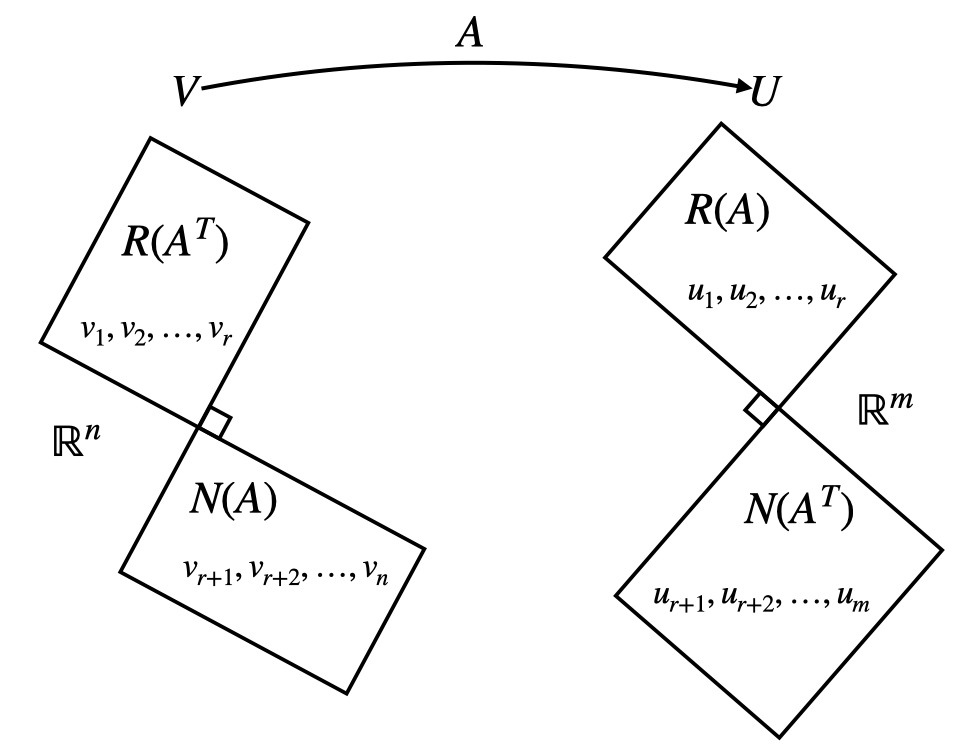
\includegraphics[width=0.5\linewidth]{figs/SVDmap.png}
\end{figure}
\end{remark}

\begin{theorem}[秩 $k$ 最佳逼近]
设 $A=U\Sigma V^H$，定义 $A_k$ 为：
\[
    A_k=\sum_{i=1}^k\sigma_iu_iv_i^H,\quad k<r
\]
则：
\begin{align*}
    &\min_{\text{rank}(B)=k}\Vert A-B\Vert_1=\Vert A-A_k\Vert_1=\sigma_{k+1}\\
    &\min_{\text{rank}(B)=k}\Vert A-B\Vert_F^2=\Vert A-A_k\Vert_F^2=\sigma_{k+1}^2+\cdots\sigma_{r}^2
\end{align*}
\end{theorem}

\begin{theorem}
设 $A=U\Sigma V^H$，则：
\begin{gather*}
    N(A)=\text{span}\{v_{r+1},v_{r+2},\ldots,v_{n}\}\\
    R(A)=\text{span}\{u_1,u_2,\ldots,u_r\}
\end{gather*}
\end{theorem}
\begin{proof}
设
\[
    A=U\Sigma V^H=\begin{bmatrix}U_1&U_2\end{bmatrix}\begin{bmatrix}\Sigma_r&O\\O&O\end{bmatrix}\begin{bmatrix}V_1^H\\V_2^H\end{bmatrix}=U_1\Sigma_rV_1^H
\]
容易验证：
\[
    U_1\Sigma_rV_1^Hx=0\iff V_1^Hx=0
\]
(1).
\begin{align*}
    N(A)&=\{x\mid Ax=0\}=\{x\mid U_1\Sigma V_1^Hx=0\}\\
    &=\{x\mid V_1^Hx=0\}=N(V_1^H)=R^{\perp}(V_1)\\
    &=R(V_2)=\text{span}\{v_{r+1},\ldots,v_n\}
\end{align*}
(2).
\begin{align*}
    &R(A)=\{y\mid y=Ax\}=\{y\mid y=U_1(\Sigma V_1^Hx)\}\subset\{y\mid y=U_1z\}=R(U_1)\\
    &R(U_1)=\{y\mid y=U_1z\}=\{y\mid y=A(V_1\Sigma_1^{-1}z)\}\subset\{y\mid y=Ax\}=R(A)\\
    \implies&R(A)=R(U_1)=\text{span}\{u_1,u_2,\ldots,u_r\}
\end{align*}
\end{proof}

\begin{theorem}[正规矩阵的奇异值分解]
设 $A$ 是正规矩阵（即 $A^HA=AA^H$），则 $A$ 酉相似于对角矩阵，即存在酉矩阵 $U$ 使得：
\[
    A=U\begin{bmatrix}
    \lambda_1&&&&&\\
    &\ddots&&&&\\
    &&\lambda_r&&&\\
    &&&0&&\\
    &&&&\ddots&\\
    &&&&&0\\
    \end{bmatrix}U^H
\]
其中 $\lambda_i$ 是 $A$ 的特征值（注意可能为负）。那么可以构造奇异值分解如下：
\[
    A=U\underbrace{\begin{bmatrix}
    |\lambda_1|&&&&&\\
    &\ddots&&&&\\
    &&|\lambda_r|&&&\\
    &&&0&&\\
    &&&&\ddots&\\
    &&&&&0\\
    \end{bmatrix}}_{\Sigma}
    \underbrace{\begin{bmatrix}
    \lambda_1/|\lambda_1|&&&&&\\
    &\ddots&&&&\\
    &&\lambda_r/|\lambda_r|&&&\\
    &&&1&&\\
    &&&&\ddots&\\
    &&&&&1\\
    \end{bmatrix}U^H}_{V^H}
\]
\end{theorem}


\begin{definition}[正交相抵]
设有矩阵 $A_{m\times n},\,B_{m\times n}$，若存在酉矩阵 $U_{m\times m},\,V_{n\times n}$ 使得 $U^HAV=B$，则称 $A$ 与 $B$ 正交相抵。
\end{definition}

\begin{property}
正交相抵是一个等价关系，即满足自反性、对称性和传递性。
\end{property}

\begin{theorem}
若 $A$ 与 $B$ 正交相抵，则 $\sigma_A=\sigma_B$.
\end{theorem}
\begin{proof}
$B=U^HAV\implies B^HB=V^HA^HUU^HAV=V^HA^HAV\implies\lambda_{B^HB}=\lambda_{A^HA}\implies \sigma_B=\sigma_A$.
\end{proof}
 \newpage
\section{特征值的估计}

\subsection{特征值的估计}

矩阵的特征值在理论上和实际应用中都是十分重要的，但是特征值的计算一般是非常麻烦的，尤其当矩阵的阶数比较高时，要精确计算出矩阵的特征值是相当困难的，因此，由矩阵元素的简单关系式估计出特征值的范围就显得尤为重要。本节将主要给出特征值的估计与圆盘定理，以及谱半径的估计。

\begin{theorem}[特征值的上界]
设 $A\in \mathbb R^{n\times n}$，令：
\[
    M=\max_{1\leq r,s\leq n}\frac{1}{2}|a_{rs}-a_{sr}|
\]
若 $\lambda$ 表示 $A$ 的任一特征值，则 $\lambda$ 的虚部 $\text{Im}(\lambda)$ 满足不等式：
\begin{align*}
    &|\text{Im}(\lambda)|\leq M\sqrt{\frac{n(n-1)}{2}}\\
    &|\text{Im}(\lambda)|\leq\frac{\Vert A-A^T\Vert_2}{2}\\
    &|\text{Im}(\lambda)|\leq\frac{\Vert A-A^T\Vert_1\cdot\sqrt{n}}{2}
\end{align*}
\end{theorem}

\begin{remark}
基本思想：任何一个实方阵都可以拆分为实对称阵和实反对称阵的和：
\[
    A=\frac{1}{2}(A+A^T)+\frac{1}{2}(A-A^T)
\]
我们知道实对称阵的特征值一定是实数，而实反对称阵的特征值一定是 0 或虚数。因此，可以认为上面的两部分分别决定了特征值的实部和虚部，这就是为什么我们关注 $M=\max\limits_{1\leq r,s\leq n}\frac{1}{2}|a_{rs}-a_{sr}|$.
\end{remark}
\begin{proof}
暂略。
\end{proof}

\begin{definition}[行对角占优]
设 $A\in\mathbb C^{n\times n}$，令：
\[
    R_r(A)=\sum_{s=1,s\neq r}^n|a_{rs}|,\quad r=1,\ldots,n
\]
若 $|a_{rr}|>R_{r}(A),\ \forall\ r=1,\ldots,n$，则称矩阵 $A$ 按行对角占优。
\end{definition}

\begin{theorem}
行对角占优阵一定可逆。
\end{theorem}
\begin{proof}
假设 $A$ 不可逆，则其列线性相关，即存在不全为零的 $k_1,\ldots,k_n$ 使得 $k_1a_1+\cdots+k_na_n=0$. 设 $k_r$ 是其中模长最大的，考虑第 $r$ 个分量：
\[
    k_1a_{r1}+\cdots+k_na_{rn}=0\implies a_{rr}=-\sum_{s=1,s\neq r}^n\frac{k_s}{k_r}a_{rs}
\]
于是：
\[
    |a_{rr}|\leq \sum_{s=1,s\neq r}^n\frac{|k_s|}{|k_r|}|a_{rs}|\leq \sum_{s=1,s\neq r}^n|a_{rs}|
\]
与 $A$ 行对角占优矛盾，故假设不成立。
\end{proof}

\begin{theorem}[行对角占优阵的行列式的上下界]
设 $A\in\mathbb C^{n\times n}$ 且按行对角占优，令：
\[
    M_r=|a_{rr}|+\sum_{s=r+1}^n|a_{rs}|,\quad m_r=|a_{rr}|-\sum_{s=r+1}^n|a_{rs}|,\quad r=1,\ldots,n
\]
则：
\[
    0<\prod_{r=1}^n m_r\leq |\det A|=\prod_{r=1}^n|\lambda_r(A)|\leq\prod_{r=1}^n M_r
\]
当 $a_{rs}=0\ (s>r)$ 时等号成立。
\end{theorem}
\begin{proof}
对 $A$ 分块：
\[
    A=\left[\begin{array}{c:ccc}
    a_{11}&a_{12}&\cdots&a_{1n}\\
    \hdashline a_{21}&&&\\
    \vdots&&A_1&\\
    a_{n1}&&&\\
    \end{array}\right]
\]
设 $x=(\xi_2,\ldots,\xi_n)^T$ 且满足：
\[
    \begin{bmatrix}a_{21}\\\vdots\\a_{n1}\end{bmatrix}+A_1\begin{bmatrix}\xi_2\\\vdots\\\xi_n\end{bmatrix}=0
\]
则有 $|\xi_k|=\max\{|\xi_2|,\ldots,|\xi_n|\}<1$，证明方式与上面证明行对角占优矩阵一定可逆的方式类似。
于是，利用行列式的性质，有：
\[
    \det(A)=\det\left(A\begin{bmatrix}1&0\\x&I_{n-1}\end{bmatrix}\right)=\det\left(
    \left[\begin{array}{c:ccc}
    b_{11}&a_{12}&\cdots&a_{1n}\\
    \hdashline&&&\\
    0&&A_1&\\
    &&&
    \end{array}\right]
    \right)=|b_{11}|\cdot\det(A_1)
\]
其中
\[
    b_{11}=a_{11}+\sum_{s=2}^na_{1s}\xi_s,\quad|\xi_s|<1
\]
因此 $m_1\leq|b_{11}|\leq M_1$.  然后递归地对 $A_1$ 做类似推导即可。
\end{proof}

\begin{theorem}[Hadamard 不等式]
设 $A\in\mathbb C^{n\times n}$，则有：
\[
    |\det(A)|=\prod_{r=1}^n|\lambda_r(A)|\leq\left[\prod_{s=1}^n\left(\sum_{r=1}^n|a_{rs}|^2\right)\right]^{1/2}
\]
\end{theorem}
\begin{remark}[直观解释]
平行多面体的体积小于等于将其拉成正立方体的体积。
\end{remark}
\begin{proof}
若 $a_1,\ldots,a_n$ 线性无关，则显然成立；否则，进行 Gram-Schmidt 正交化过程，写作矩阵形式：
\[
    (a_1,a_2,\ldots,a_n)=(b_1,b_2,\ldots,b_n)\begin{bmatrix}1&k_{21}&\cdots&k_{n1}\\&1&\cdots&k_{n2}\\&&\ddots&\vdots\\&&&1\end{bmatrix}
\]
易知 $\Vert a_i\Vert^2\geq\Vert b_i\Vert^2$，于是：
\[
    |\det(A)|^2=|\det(B)|^2=\det(B^HB)=\Vert b_1\Vert^2\cdots\Vert b_n\Vert^2\leq\Vert a_1\Vert^2\cdots\Vert a_n\Vert^2
\]
\end{proof}

\begin{theorem}[Schur 不等式，特征值模长平方和的界]
设 $A\in\mathbb C^{n\times n}$ 的特征值为 $\lambda_1,\ldots,\lambda_n$，则：
\[
    \sum_{r=1}^n|\lambda_r|^2\leq\sum_{r=1}^n\sum_{s=1}^n|a_{rs}|^2=\Vert A\Vert_F^2
\]
\end{theorem}
\begin{proof}
根据 Schur 定理 \ref{thm:schur}，存在酉矩阵 $U$ 使得 $A=UTU^H$，其中 $T$ 为上三角矩阵，对角元素为 $A$ 的特征值，且：
\[
    \sum_{r=1}^n|\lambda_r|^2=\sum_{k=1}^n|t_{kk}|^2\leq\sum_{r=1}^n\sum_{s=1}^n|t_{rs}|^2=\text{tr}(T^HT)=\text{tr}(A^HA)
\]
\end{proof}

\begin{definition}[行盖尔圆]
设 $A\in\mathbb C^{m\times n}$，记第 $i$ 个行盖尔圆为：
\[
    S_i=\{z\mid |z-a_{ii}|\leq R_i,\,z\in\mathbb C\}
\]
其中 $R_i=R_i(A)=\sum_{j\neq i}|a_{ij}|$.
\end{definition}

\begin{theorem}[圆盘定理 1]
$A$ 的所有特征值在其 $n$ 个盖尔圆的并集之内，即：
\[
    \lambda\in S=\bigcup_{i=1}^nS_i=\bigcup_{i=1}^n\{z\mid |z-a_{ii}|\leq R_i,\,z\in\mathbb C\}
\]
\end{theorem}
\begin{proof}
设 $Ax=\lambda x$，写作分量形式：
\[
    \sum_{j=1}^na_{ij}x_j=\lambda x_i\implies (\lambda-a_{ii})x_i=\sum_{j\neq i}a_{ij}x_j
\]
设 $x_t$ 为 $x$ 各分量中模最大的那个，则 $x_t\neq 0$，上式取 $i=t$ 后两边同时除以 $x_t$ 并取模得：
\[
    |\lambda-a_{tt}|=\sum_{j\neq t}|a_{tj}|\left|\frac{x_j}{x_t}\right|\leq\sum_{j\neq t}|a_{tj}|=R_t(A)
\]
因此 $\lambda\in S_t$.  于是任意特征值 $\lambda\in\bigcup_{i=1}^n S_i$.
\end{proof}

\begin{remark}
圆盘定理 1 说明，特征值 $\lambda$ 属于特征向量最大分量的下标对应的盖尔圆。
\end{remark}

\begin{theorem}[圆盘定理 2]
设矩阵 $A$ 的 $n$ 个盖尔圆有 $k$ 个互相连通并且与其余 $n-k$ 个不相交，则这个连通区域中恰有 $k$ 个特征值。
\end{theorem}
\begin{remark}
设 $A=D+B$，其中 $D$ 为对角矩阵。设 $A(t)=D+tB$，则当 $t=0$ 时，所有盖尔圆都是点，也就是特征值；当 $t$ 从 $0$ 到 $1$ 连续变化时，盖尔圆越来越大，而特征值也是\textbf{连续}变化的，所以 $t=1$ 时特征值只能在其连通区域内，不可能跳跃到不连通的另一个区域中。从这个角度也可以知道，当两个盖尔圆相切时，其特征值最多到达切点处。
\end{remark}

\begin{corollary}
若 $n$ 阶矩阵 $A$ 的 $n$ 个盖尔圆两两互不相交（都是孤立的），则 $A$ 相似于对角矩阵。
\end{corollary}

\begin{corollary}
设 $n$ 阶实矩阵 $A$ 的 $n$ 个盖尔圆两两互不相交，则 $A$ 的特征值全为实数。
\end{corollary}

\begin{proof}
由于 $A$ 为实矩阵，故所有盖尔圆的圆心都在实轴上。若 $A$ 有复特征值，则必有与之关于实轴对称的共轭复对称值，与其在同一个盖尔圆中。由于盖尔圆两两互不相交，且一个孤立盖尔圆内只能有一个特征值，所以 $A$ 的特征值只能都是实数。
\end{proof}

\begin{definition}[列盖尔圆]
设 $A\in\mathbb C^{m\times n}$，记第 $j$ 个列盖尔圆为：
\[
    G_j=\{z\mid |z-a_{jj}|\leq R'_j,\,z\in\mathbb C\}
\]
其中 $R'_j=R'_j(A)=\sum_{i\neq j}|a_{ij}|$.
\end{definition}

\begin{corollary}
列盖尔圆有与行盖尔圆类似的圆盘定理。结合二者可知，$A$ 的所有特征值都在以下平面区域之中：
\[
T=\left(\bigcup_{i=1}^nS_i\right)\cap\left(\bigcup_{j=1}^nG_j\right)
\]
\end{corollary}

\begin{theorem}
相似矩阵的盖尔圆的圆心相同、半径不同。
\end{theorem}
\begin{proof}
由于 $B=P^{-1}AP$ 的第 $i$ 行第 $j$ 列元素为 $a_{ij}p_i/p_j$，所以对于 $B$：
\[
    R_i=\sum_{j\neq i}\left\vert a_{ij}\cdot\frac{p_i}{p_j}\right\vert
\]
而圆心依旧是 $a_{ii}\cdot p_i/p_i=a_{ii}$.
\end{proof}

\begin{remark}
这个定理可以用于隔离特征值：取 $P=\text{diag}(p_1,\ldots,p_n),\,p_i>0$，若想要缩小半径，则将对应元素设置得大一些，这样原本相交的盖尔圆就能被隔离开了。
\end{remark}

\begin{theorem}
设 $A$ 为 $n$ 阶正规矩阵，则：
\[
    \rho(A)=\Vert A\Vert_2=\sqrt{\lambda_{A^HA}}
\]
其中 $\lambda_{A^HA}$ 为 $A^HA$ 的最大特征值。
\end{theorem}
\begin{proof}
设 $A$ 的特征值为 $\lambda_1,\ldots,\lambda_n$，存在酉矩阵 $U$ 使得：
\[
    U^HAU=\text{diag}(\lambda_1,\ldots,\lambda_n)
\]
于是：
\[
    U^HA^HU=\text{diag}(\bar\lambda_1,\ldots,\bar\lambda_n)
\]
因此：
\[
    U^HA^HAU=\text{diag}(|\lambda_1|^2,\ldots,|\lambda_n|^2)
\]
故 $A^HA$ 的特征值为 $|\lambda_1|^2,\ldots,|\lambda_n|^2$，记 $\lambda_{A^HA}=\max_{1\leq i\leq n}|\lambda_i|^2$，则：
\[
    \Vert A\Vert_2=\sqrt{\lambda_{A^HA}}=\max_{1\leq i\leq n}|\lambda_i|=\rho(A)
\]
\end{proof}

\begin{remark}
由于实对称矩阵、实反对称矩阵、正交矩阵、酉矩阵、Hermite 矩阵、反 Hermite 矩阵、对角矩阵都是正规矩阵，所以它们都有性质 $\rho(A)=\Vert A\Vert_2$.
\end{remark}
\begin{remark}
事实上，从上述证明过程可以看出，正规矩阵的奇异值等于特征值的模长的平方（可以一一对应上）。
\end{remark}


\subsection{广义特征值问题}

\begin{definition}[广义特征值]
设 $A,B$ 为 $n$ 阶方阵，若存在数 $\lambda$，使得方程 $Ax=\lambda Bx$ 存在非零解，则称 $\lambda$ 为 $A$ 相对于 $B$ 的广义特征值，$x$ 为 $A$ 相对于 $B$ 的属于广义特征值 $\lambda$ 的特征向量。
\end{definition}

\noindent\textbf{广义特征值求解}：解 $(\lambda B-A)x=0\iff\det(\lambda B-A)=0$ 即可。注意这里的特征多项式 $\det(\lambda B-A)$ 不一定是 $n$ 阶多项式，从而不一定有 $n$ 个根。

\vskip 6pt \noindent\textbf{以下仅考虑 $A,B$ 是正定 Hermite 矩阵的情形}。

\begin{definition}[按 $B$ 标准正交化]
若向量系 $(x_1,\ldots,x_n)$ 满足：
\[
    (x_i,Bx_j)=\delta_{ij}
\]
称该向量系为按 $B$ 标准正交化的向量系。
\end{definition}

\begin{definition}[广义特征值的等价表述 1]
由于 $B$ 正定，因此可逆，故：
\[
    Ax=\lambda Bx\implies B^{-1}Ax=\lambda x
\]
转化为了标准特征值问题。但一般而言 $B^{-1}A$ 不再是 Hermite 矩阵。
\end{definition}

\begin{definition}[广义特征值的等价表述 2]
由于 $B$ 为 Hermite 矩阵，因此存在 Cholesky 分解，$B=GG^H$，其中 $G$ 满秩，于是：
\[
    Ax=\lambda Bx\implies Ax=\lambda GG^Hx
\]
令 $y=G^Hx$，则：
\[
    G^{-1}A(G^H)^{-1}y=\lambda y
\]
转化为了标准特征值问题，且 $G^{-1}A(G^H)^{-1}$ 仍然是 Hermite 矩阵，因此广义特征值为实数，设为 $\lambda_1\leq\cdots\leq\lambda_n$，且存在一组正交归一化的特征向量 $(y_1,\ldots,y_n)$，即：
\begin{align*}
    &G^{-1}A(G^H)^{-1}y_i=\lambda y_i\\
    &y_i^Hy_j=\delta_{ij}
\end{align*}
将 $y$ 还原为 $x$，则：
\[
    y_i^Hy_j=(G^Hx_i)^H(G^Hx_j)=x_i^HGG^Hx_j=x_i^HBx_j=\delta_{ij}
\]
即 $(x_1,\ldots,x_n)$ 按 $B$ 标准正交。
\end{definition}


\subsection{对称矩阵特征值的极性}

我们首先讨论实对称矩阵特征值的极性与 Rayleigh 商。本节中记实对称矩阵 $A$ 的特征值按大小排列为 $\lambda_1\leq\lambda_2\leq\cdots\leq\lambda_n$，对应\textbf{标准正交}特征向量系为 $p_1,p_2,\ldots,p_n$.

\begin{remark}
将 Rayleigh 商定义在实对称矩阵上是为了保证特征值一定是实数，这样才可以比较。
\end{remark}

\begin{definition}[Rayleigh 商]
设 $A$ 是 $n$ 阶实对称矩阵，$x\in\mathbb R^n$，定义矩阵 $A$ 的 Rayleigh 商为：
\[
    R(x)=\frac{x^TAx}{x^Tx},\quad x\neq 0
\]
\end{definition}
\begin{theorem}
设 $A$ 为实对称矩阵，则：
\[
    \min_{x\neq 0}R(x)=\lambda_1,\quad\max_{x\neq 0}R(x)=\lambda_n
\]
\end{theorem}
\begin{proof}[证明 1]
任取 $x\neq 0$，依标准正交特征向量系分解 $x=c_1p_1+\cdots+c_np_n$，则：
\[
    x^Tx=c_1^2+\cdots+c_n^2,\quad x^TAx=c_1^2\lambda_1+\cdots+c_n^2\lambda_n
\]
故：
\[
    R(x)=k_1\lambda_1+\cdots+k_n\lambda_n,\quad\text{where}\; k_i=\frac{c_i^2}{c_1^2+\cdots+c_n^2}
\]
容易推出 $\lambda_1\leq R(x)\leq\lambda_n$，且 $R(p_1)=\lambda_1,\,R(p_n)=\lambda_n$.
\end{proof}
\begin{proof}[证明 2（梯度法）]
取对数 $\ln R(x)=\ln (x^TAx)-\ln(x^Tx)$，求导并令为零：
\[
    \frac{\mathrm d\ln R(x)}{\mathrm dx}=\frac{2Ax}{x^TAx}-\frac{2x}{x^Tx}=0\implies Ax=R(x)x
\]
因此极值点处 $R(x)$ 为 $A$ 的特征值，$x$ 为对应特征向量。于是最小值为最小特征值 $\lambda_1$，最大值为最大特征值 $\lambda_n$.
\end{proof}
\begin{proof}[证明 3（拉格朗日乘子法）]
原问题可等价转换为如下带约束优化问题：
\[
    \min_{x^Tx=1} x^TAx,\quad\max_{x^Tx=1} x^TAx
\]
引入拉格朗日函数：
\[
    L(x,\lambda)=x^TAx-\lambda x^Tx
\]
求导并令为零：
\[
    \frac{\partial L(x,\lambda)}{\partial x}=2Ax-2\lambda x=0\implies Ax=\lambda x
\]
这意味着极值点 $x$ 为 $A$ 的特征向量，$\lambda$ 是对应特征值。此时，极值正好也是 $x^TAx=\lambda x^Tx=\lambda$. 因此，原问题最小值就是 $A$ 的最小特征值 $\lambda_1$，最大值就是 $A$ 的最大特征值 $\lambda_n$.
\end{proof}

\begin{remark}
由于 $x$ 模长不影响 $R(x)$，所以上述定理也常常写作：
\[
    \min_{\Vert x\Vert_2=1}x^TAx=\lambda_1,\quad\max_{\Vert x\Vert_2=1}x^TAx=\lambda_n
\]
下文视情况两种写法都可能出现。
\end{remark}

\begin{theorem}[Rayleigh 商中的向量扩展为矩阵]
设 $A$ 为实对称矩阵，则对于任意的 $1\leq r\leq n$ 有：
\[
    \min_{X^TX=I_r}\text{tr}(X^TAX)=\lambda_1+\cdots+\lambda_r
\]
\end{theorem}
\begin{proof}
对 $A$ 作谱分解 $A=P\Lambda P^T$，其中 $P$ 为正交矩阵，$\Lambda=\text{diag}(\lambda_1,\ldots,\lambda_n)$. 记 $B=P^TX$，则问题转化为对角矩阵情形，即求证：
\[
    \min_{B^TB=I_r}\text{tr}(B^T\Lambda B)=\lambda_1+\cdots+\lambda_r
\]
记 $BB^T$ 的对角元素为 $B_{11},\ldots,B_{nn}$，则可以证明在 $B^TB=I$ 的条件下，$0\leq B_{ii}\leq 1$.  因此：
\[
    \text{tr}(B^T\Lambda B)=\text{tr}(\Lambda BB^T)=\lambda_1B_{11}+\cdots+\lambda_n B_{nn}
\]
所以这是一个关于 $B_{11},\ldots,B_{nn}$ 的线性约束下的线性问题，最小值必然在约束区域的顶点处取得。显然这个顶点应该是 $B_{11}=\cdots=B_{rr}=1$，$B_{r+1,r+1}=\cdots=B_{nn}=0$，此时取到最小值 $\lambda_1+\cdots+\lambda_r$.
\end{proof}

\begin{theorem}
\label{thm:minmaxR}
设 $x\in L(p_r,p_{r+1},\ldots,p_s),\,1\leq r\leq s\leq n$，则：
\[
    \min_{x\neq 0}R(x)=\lambda_r,\quad\max_{x\neq 0}R(x)=\lambda_s
\]
\end{theorem}
\begin{proof}
证明与前面的定理证明类似。
\end{proof}
\begin{remark}
这个定理表明 Rayleigh 商在特征向量张成的子空间中的极值就是对应最大最小特征值。但是在实际应用中，特征向量张成的子空间并不好找，所以下面的 Courant-Fischer 定理只限制子空间维数为 $k$，再对所有 $k$ 维子空间求极值。
\end{remark}

\begin{theorem}[Courant-Fischer]
设 $V_k$ 表示 $\mathbb R^n$ 中的任意一个 $k$ 维子空间，则：
\[
    \lambda_k=\min_{V_k}\max_{x\in V_k,x\neq0}R(x)
\]
或写作：
\[
    \lambda_k=\min_{V_k}\max_{x\in V_k,\Vert x\Vert_2=1}x^TAx
\]
\end{theorem}
\begin{proof}
取 $V_k=L(p_1,\ldots,p_k)$，根据定理 \ref{thm:minmaxR} 有：
\[
    \max_{x\neq 0}R(x)=\lambda_k
\]
因此下面只需要证明对所有 $V_k$，$\max\limits_{x\neq 0}R(x)\geq \lambda_k$.
构造 $R^n$ 的 $n-k+1$ 维子空间 $W_k=L(p_k,p_{k+1},\ldots,p_n)$，则任一 $V_k$ 与 $W_k$ 必有交集。取非零向量 $x\in V_k\cap W_k$，设 $x=c_kp_k+\cdots+c_np_n$，则：
\[
    R(x)=\frac{c_k^2\lambda_k+\cdots+c_n^2\lambda_n}{c_k^2+\cdots c_n^2}\geq \lambda_k
\]
\end{proof}

\begin{corollary}
将 $A$ 替换成 $-A$，能立刻得到如下结论：
\[
    \lambda_{n-k+1}=\max_{V_k}\min_{x\in V_k,x\neq0}R(x)
\]
\end{corollary}

\begin{theorem}
\label{thm:AAQ}
设实对称矩阵 $A$ 和 $A+Q$ 的特征值分别为 $\lambda_1\leq\cdots\leq\lambda_n$ 和 $\mu_1\leq\cdots\leq\mu_n$，则：
$$
|\lambda_i-\mu_i|\leq \Vert Q\Vert_2
$$
\end{theorem}
\begin{proof}
利用 Courant-Fischer 定理，
\begin{align*}
    \mu_i+\Vert Q\Vert_2&=\min_{V_i}\max_{x\in V_i,\Vert x\Vert_2=1}x^T(A+Q)x+\Vert Q\Vert_2I\\
    &=\min_{V_i}\max_{x\in V_i,\Vert x\Vert_2=1}x^T(A+Q+\Vert Q\Vert_2I)x\\
    &\geq\min_{V_i}\max_{x\in V_i,\Vert x\Vert_2=1}x^TAx\\
    &=\lambda_i
\end{align*}
不等式是因为 $Q+\Vert Q\Vert_2I$ 为半正定矩阵。另一个方向可以进行类似的证明（用 $Q-\Vert Q\Vert_2I$ 为半负定矩阵）。
\end{proof}

\begin{remark}
为什么 $Q+\Vert Q\Vert_2I$ 是半正定矩阵？对 $Q$ 进行谱分解 $Q=P\Lambda P^T$，则：
\[
    Q+\Vert Q\Vert_2I=P\Lambda P^T+\Vert\Lambda\Vert_2I=P(\Lambda +\Vert\Lambda\Vert_2I)P^T
\]
因此只需要证明对角矩阵 $\Lambda +\Vert\Lambda\Vert_2I$ 是半正定矩阵。由于 $\Vert\Lambda\Vert_2=\rho(\Lambda)$，因此其对角元素一定非负，这样就完成了证明。
\end{remark}

\begin{definition}[广义 Rayleigh 商]
设 $A,B$ 为 $n$ 阶实对称矩阵，\textbf{且 $B$ 正定}，定义矩阵 $A$ 相对于矩阵 $B$ 的广义 Rayleigh 商为：
\[
    R(x)=\frac{x^TAx}{x^TBx},\quad x\neq 0
\]
\end{definition}
\begin{theorem}
非零向量 $x_0$ 是 $R(x)$ 的驻点的充要条件是 $x_0$ 为 $Ax=\lambda Bx$ 的属于特征值 $\lambda$ 的特征向量。
\end{theorem}

\begin{corollary}
若 $x_0$ 是 $A$ 相对于 $B$ 的特征向量，则 $R(x_0)$ 是与之对应的特征值。
\end{corollary}

\begin{theorem}[Courant-Fischer 定理在广义特征值上的扩展]
广义特征值问题有如下极小极大性质：
\begin{align*}
    \lambda_k&=\min_{V_k}\max_{x\in V_k,x\neq 0}R(x)\\
    \lambda_{n-k+1}&=\max_{V_k}\min_{x\in V_k,x\neq0}R(x)
\end{align*}
\end{theorem}

\begin{theorem}[矩阵奇异值的极性]
设 $A\in\mathbb R^{m\times n}_r$ 的奇异值为：
\[
    0=\sigma_1=\sigma_2=\cdots=\sigma_{n-r}<\sigma_{n-r+1}\leq\cdots\leq\sigma_n
\]
$A+Q\in\mathbb R^{m\times n}_{r'}$ 的奇异值为：
\[
    0=\tau_1=\tau_2=\cdots=\tau_{n-r'}<\tau_{n-r'+1}\leq\cdots\leq\tau_n
\]
则有：
\[
    |\sigma_i-\tau_i|\leq \Vert Q\Vert_2\quad(i=1,2,\ldots,n)
\]
\end{theorem}
\begin{remark} 
对比定理 \ref{thm:AAQ}。
\end{remark}


\subsection{矩阵的直积及其应用}

\begin{definition}[直积 / Kronecker 积]
设 $A=(a_{ij})\in\mathbb C^{m\times n}$，$B=(b_{ij})\in\mathbb C^{p\times q}$，则称 $A$ 与 $B$ 的直积（Kronecker 积）为：
\[
    A\otimes B=
    \begin{bmatrix}
    a_{11}B&a_{12}B&\cdots&a_{1n}B\\
    a_{21}B&a_{22}B&\cdots&a_{2n}B\\
    \vdots&\vdots&\ddots&\vdots\\
    a_{m1}B&a_{m2}B&\cdots&a_{mn}B\\
    \end{bmatrix}\in\mathbb C^{mp\times nq}
\]
换句话说，$a_{ij}b_{kl}$ 放在 $A\otimes B$ 的 $((i-1)m+k,(j-1)n+l)$ 处。
\end{definition}

\begin{property}
$k(A\otimes B)=(kA)\otimes B=A\otimes(kB)$
\end{property}

\begin{property}
若 $A,B$ 同阶，则 $(A+B)\otimes C=A\otimes C+B\otimes C$，$C\otimes(A+B)=C\otimes A+C\otimes B$.
\end{property}

\begin{property}
$(A\otimes B)\otimes C=A\otimes(B\otimes C)$
\end{property}
\begin{proof}[证明思路]
证明 $a_{ij}b_{kl}c_{uv}$ 在同一个位置。
\end{proof}

\begin{property}
$(A\otimes B)(C\otimes D)=AC\otimes BD$
\end{property}
\begin{proof}[证明思路]
直接展开。
\end{proof}

\begin{property}
$(A_1\otimes\cdots\otimes A_l)(B_1\otimes\cdots\otimes B_l)=A_1B_1\otimes\cdots\otimes A_lB_l$
\end{property}

\begin{property}
$(A_1\otimes B_1)\cdots(A_l\otimes B_l)=(A_1\cdots A_l)\otimes(B_1\cdots B_l)$
\end{property}

\begin{property}
$(A\otimes B)^{-1}=A^{-1}\otimes B^{-1}$
\end{property}
\begin{proof}
$(A\otimes B)(A^{-1}\otimes B^{-1})=(AA^{-1})\otimes(BB^{-1})=I$.
\end{proof}

\begin{property}
若 $A,B$ 为三角矩阵，则 $A\otimes B$ 也是三角矩阵。
\end{property}

\begin{property}
$(A\otimes B)^H=A^H\otimes B^H$
\end{property}

\begin{property}
设 $A_{m\times m}$ 和 $B_{n\times n}$ 都是酉矩阵，则 $A\otimes B$ 也是酉矩阵。
\end{property}

\begin{property}
$\text{rank}(A\otimes B)=\text{rank}(A)\cdot\text{rank}(B)$
\end{property}
\begin{proof}    
对 $A,B$ 作奇异值分解 $A=U_A\Sigma_AV_A^H,\,B=U_B\Sigma_BV_B^H$，则：
\[
    A\otimes B=(U_A\otimes U_B)(\Sigma_A\otimes\Sigma_B)(V_A\otimes V_B)^H
\]
按定义易知 $\Sigma_A\otimes \Sigma_B$ 有 $\text{rank}(A)\cdot\text{rank}(B)$ 个非零元。证毕。
\end{proof}

\begin{property}
$\text{tr}(A\otimes B)=\text{tr}(A)\cdot\text{tr}(B)$.
\end{property}
\begin{proof}[证明思路]
直接展开。
\end{proof}

\begin{property}
对于\textbf{方阵} $A\in\mathbb C^{m\times m},\,B\in\mathbb C^{n\times n}$，有 $A\otimes B$ 相似于 $B\otimes A$.
\end{property}

\begin{definition}[拉直算子]
设 $A=(a_1,a_2,\ldots,a_n)$，定义\textbf{列拉直}为：
\[
    \text{vec}(A)=\begin{bmatrix}a_1\\a_2\\\vdots\\a_n\end{bmatrix}=\sum_{j=1}^ne_j\otimes (Ae_j)
\]
类似地，设 $A=\begin{bmatrix}a_1^T\\a_2^T\\\vdots\\a_m^T\end{bmatrix}$，定义\textbf{行拉直}为：
\[
    \overline{\text{vec}}(A)=\begin{bmatrix}a_1\\a_2\\\vdots\\a_m\end{bmatrix}=\sum_{i=1}^me_i\otimes(A^Te_i)
\]
显然有：$\overline{\text{vec}}(A)=\text{vec}(A^T)$.
\end{definition}

\begin{theorem}
设 $A\in\mathbb C^{m\times n},X\in\mathbb C^{n\times p},B\in\mathbb C^{p\times q}$，则：
\begin{align*}
    &\text{vec}(AXB)=(B^T\otimes A)\text{vec}(X)\\
    &\overline{\text{vec}}(AXB)=(A\otimes B^T)\overline{\text{vec}}(X)
\end{align*}
\end{theorem}
\begin{proof}
这里采用代数形式，采用展开形式也能证：
\begin{align*}
    \text{vec}(AXB)&=\sum_{j=1}^qe_j\otimes(AXBe_j)=\sum_{j=1}^qe_j\otimes\left(AX\left(\sum_{k=1}^pe_ke_k^T\right)Be_j\right)\\
    &=\sum_{j=1}^q\sum_{k=1}^pe_j\otimes (AXe_k{\color{purple}e_k^TBe_j})=\sum_{k=1}^p\sum_{j=1}^q(e_j{\color{purple}e_j^TB^Te_k})\otimes (AXe_k)\\
    &=\sum_{k=1}^p(B^Te_k)\otimes (AXe_k)=\sum_{k=1}^p(B^T\otimes A)(e_k\otimes Xe_k)=(B^T\otimes A)\text{vec}(X)
\end{align*}
推导过程中注意紫色部分是一个数，可以转置并移动到直积的另一边去。
行展开类似，或者直接取转置即可。
\end{proof}

\begin{definition}[以矩阵直积定义方幂]
设 $A\in\mathbb C^{m\times n}$，定义 $A^{[1]}=A,\,A^{[k+1]}=A^{[k]}\otimes A,\,k=1,2,\ldots$.
\end{definition}

\begin{property}
$(AB)^{[k]}=A^{[k]}B^{[k]}$. 利用直积的性质 4 容易证明。
\end{property}

\begin{definition}
对二元函数 $f(x,y)=\displaystyle\sum_{i,j=0}^lc_{ij}x^iy^j$ 及矩阵 $A\in\mathbb C^{m\times m},\,B\in\mathbb C^{n\times n}$，定义：
\[
    f(A,B)=\sum_{i,j=0}^lc_{ij}A^{i}\otimes B^{j}
\]
\end{definition}

\begin{theorem}[二元函数 $f(A,B)$ 的特征值]
设 $A_{m\times m}$ 的特征值为 $\lambda_1,\lambda_2,\ldots,\lambda_m$，$B_{n\times n}$ 的特征值为 $\mu_1,\mu_2,\ldots,\mu_n$，则 $f(A,B)$ 的全体特征值为 $f(\lambda_i,\mu_j),\,i=1,2,\ldots,m,j=1,2,\ldots,n$.
\end{theorem}
\begin{proof}
将 $A,B$ 相似上三角化 $A=P_AR_AP_A^{-1},\,B=P_BR_BP_B^{-1}$，其中 $R_A,R_B$ 为上三角矩阵。那么 $A^i=P_AR_A^iP_A^{-1},\,B=P_BR_B^iP_B^{-1}$，于是：
\begin{align*}
    f(A,B)&=\sum_{i,j=0}^lc_{ij}(P_AR_A^iP_A^{-1})\otimes(P_BR_B^jP_B^{-1})\\
    &=\sum_{i,j=0}^lc_{ij}(P_A\otimes P_B)(R_A^i\otimes R_B^j)(P_A^{-1}\otimes P_B^{-1})\\
    &=(P_A\otimes P_B)\left(\sum_{i,j=0}^lc_{ij}R_A^i\otimes R_B^j\right)(P_A\otimes P_B)^{-1}\\
\end{align*}
由于 $R_A^i\otimes R_B^j$ 是上三角矩阵，其对角元 $\{\lambda_r^i\mu_s^j\mid r=1,\ldots,m,s=1,\ldots,n\}$ 就是所有特征值，故 $f(A,B)$ 全体特征值为：
\[
    \text{diag}\left(\sum_{i,j=0}^{l}c_{ij}R_A^i\otimes R_B^j\right)=\left\{\sum_{i,j=0}^lc_{ij}\lambda_r^i\mu_s^j\mid r,s\right\}=\{f(\lambda_r,\mu_s)\mid r,s\}
\]
\end{proof}


\begin{corollary}
$A\otimes B$ 的全体特征值为 $\{\lambda_i\mu_j\mid i=1,\ldots,m,j=1,\ldots,n\}$.
\end{corollary}

\begin{corollary}
$\det(A\otimes B)=(\det A)^n(\det B)^m$.
\end{corollary}
\begin{proof}
$\det(A\otimes B)=\prod_{i=1}^m\prod_{j=1}^n\lambda_i\mu_j=(\prod_{i=1}^m\lambda_i^n)(\prod_{j=1}^n\mu_j^m)=(\det A)^n(\det B)^m$.
\end{proof}

\begin{corollary}
$\text{tr}(A\otimes B)=(\text{tr}A)(\text{tr}B)$.
\end{corollary}

下面我们来看矩阵方程及相关定理。

\begin{theorem}
\[
    \sum_{i=1}^lA_iXB_i=F\quad\text{有解}\quad\iff\quad
    \overline{\text{vec}}(F)\in R\left(\sum_{i=1}^lA_i\otimes B_i^T\right)
\]
\end{theorem}
\begin{proof}
两边同时进行行拉直，得：
\[
    \sum_{i=1}^l(A_i\otimes B_i^T)\overline{\text{vec}}(X)=\overline{\text{vec}}(F)
\]
于是结论显然成立。
\end{proof}

\begin{remark}
遇到形如 $\displaystyle\sum_{i=1}^lA_iXB_i=F$ 的矩阵方程，其中 $X$ 为未知量，考虑两边同时行拉直。
\end{remark}

\begin{theorem}
设 $A_{m\times m}$ 的特征值为 $\lambda_1,\ldots,\lambda_m$，$B_{n\times n}$ 的特征值为 $\mu_1,\ldots,\mu_n$，则方程 $AX+XB=F$ 有唯一解的充要条件是：
\[
    \lambda_i+\mu_j\neq 0,\,(i=1,\ldots,m,\,j=1,\ldots,n)
\]
\end{theorem}
\begin{proof}
两边同时进行行拉直，得：
\[
    (A\otimes I+I\otimes B^T)\overline{\text{vec}}(X)=\overline{\text{vec}}(F)
\]
要使该方程有唯一解，则系数矩阵特征值非零。根据上文的定理，$A\otimes I+I\otimes B^T$ 的特征值为 $\lambda_i+\mu_j$，因此命题成立。证毕。
\end{proof}

\begin{corollary}
$AX+XB=O$ 有非零解的充要条件是存在 $i_0,j_0$ 使得 $\lambda_{i_0}+\mu_{j_0}=0$.
\end{corollary}

\begin{corollary}
$AX-XA=O$ 一定有非零解。
\end{corollary}

\begin{theorem}
设 $A_{m\times m}$ 的特征值为 $\lambda_1,\ldots,\lambda_m$，$B_{n\times n}$ 的特征值为 $\mu_1,\ldots,\mu_n$，则方程 $\displaystyle\sum_{k=0}^lA^kXB^k=F$ 有唯一解的充要条件是：
\[
    1+(\lambda_i\mu_j)+\cdots+(\lambda_i\mu_j)^l\neq0
\]
\end{theorem}
\begin{proof}
两边同时进行行拉直，得：
\[
    \sum_{k=0}^l\left(A^k\otimes (B^k)^T\right)\overline{\text{vec}}(X)=\overline{\text{vec}}(F)
\]
要使该方程有唯一解，则系数矩阵特征值非零。取 $f(x,y)=\displaystyle\sum_{k=0}^lx^ky^k$，则系数矩阵为 $f(A,B^T)$，因此特征值为 $f(\lambda_i,\mu_j)=1+(\lambda_i\mu_j)+\cdots+(\lambda_i\mu_j)^l$.
\end{proof}
 \newpage
\section{广义逆矩阵}

\subsection{投影矩阵及其应用}

\begin{definition}[投影算子]
设 $\mathbb C^n=L\oplus M$，则对于任意 $x\in\mathbb C^n$ 有唯一分解 $x=y+z,\,y\in L,\,z\in M$.  称将 $x$ 变为 $y$ 的变换为沿着 $M$ 到 $L$ 的投影算子，记作 $P_{L,M}$，即：
\[P_{L,M}x=y\]
\begin{figure}[H]
    \centering
    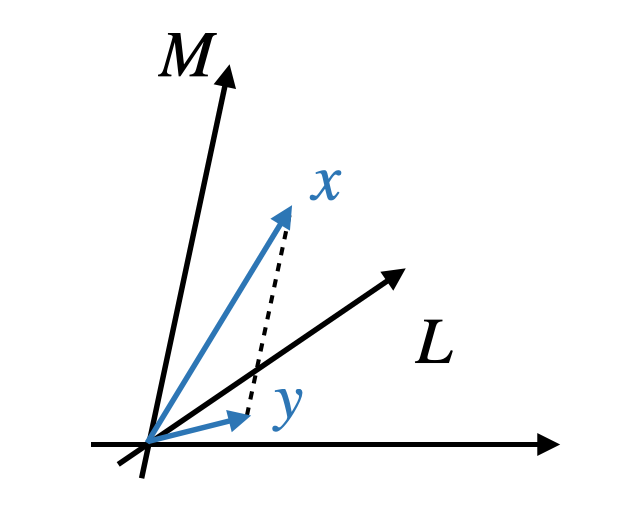
\includegraphics[width=0.2\linewidth]{figs/proj.png}
\end{figure}
\end{definition}

\begin{property}
$R(P_{L,M})=L,\,N(P_{L,M})=M$. 注意 $x-y\in M$.
\end{property}

\begin{definition}[投影矩阵]
投影算子 $P_{L,M}$ 在 $\mathbb C^n$ 的基 $(e_1,\ldots,e_n)$ 下的矩阵称为投影矩阵。
\end{definition}

\begin{lemma}
设 $A\in\mathbb C^{n\times n}$ 是幂等矩阵，即 $A^2=A$，则：
\[N(A)=R(I-A)\]
\end{lemma}
\begin{proof}
任取 $x\in N(A)$，则 $Ax=0$，则 $x=Ax+(I-A)x=(I-A)x\in R(I-A)$，因此 $N(A)\subset R(I-A)$；
任取 $y\in\mathbb C^n$，$A(I-A)y=(A-A^2)y=0$，故 $(I-A)y\in N(A)$，故 $R(I-A)\subset N(A)$；
综上，$N(A)=R(I-A)$.
\end{proof}

\begin{theorem}[投影与幂等]
\label{thm:proj-idem}
矩阵 $P$ 为投影矩阵的充要条件是 $P$ 为幂等矩阵，即：
\[
    P_{n\times n}=P_{L,M}\iff P^2=P
\]
\end{theorem}
\begin{proof}
必要性：设 $C^n=L\oplus M$，则对于任意 $x\in\mathbb C^n$，存在唯一的分解 $x=y+z,\,y\in L,\,z\in M$.  于是 $P_{L,M}x=y$. 因此 $P_{L,M}^2x=P_{L,M}y=y=P_{L,M}x$，即 $P_{L,M}$ 是幂等的。

充分性：任意 $x\in\mathbb C^n$ 可分解为 $x=Px+(I-P)x$，根据引理知 $N(P)=R(I-P)$，又 $\mathbb C^n=R(P)\oplus N(P)$，所以这样的分解是唯一的，于是 $P=P_{R(P),N(P)}$.
\end{proof}

\noindent\textbf{计算方法}：取 $L$ 的一组基 $(q_1,\ldots,q_r)$ 和 $M$ 的一组基 $(q_{r+1},\ldots,q_n)$，则任意向量 $x\in\mathbb C^n$ 可表示为：
\[
    x=(q_1,\ldots,q_r,q_{r+1},\ldots,q_n)y=Qy
\]
于是：
\[
    P_{L,M}x=QI_ry=QI_rQ^{-1}x\implies P_{L,M}=QI_rQ^{-1}
\]
其中 $I_r$ 表示前 $r$ 个对角元为 1、其余为 0 的对角矩阵。

\begin{com}
可以看见上面的计算方法涉及到基的选取，但可以证明选取不同的基算出来的 $P_{L,M}$ 都是一样的。
假设另选一组基 $\bar Q_L=(\bar q_1,\ldots,\bar q_r)$ 和 $\bar Q_M=(\bar q_{r+1},\ldots,\bar q_n)$，设 $\bar Q_L=Q_LR_1,\,\bar Q_M=Q_MR_2$，则 $\bar Q=Q\text{diag}(R_1,R_2)$，于是：
\[
    \bar P_{L,M}=\bar Q I_r\bar Q^{-1}=Q\text{diag}(R_1,R_2)I_r\text{diag}(R_1^{-1},R_2^{-1})Q^{-1}=QI_rQ^{-1}=P_{L,M}
\]
可见 $P_{L,M}$ 与基的选取无关。
\end{com}

\begin{definition}[正交投影算子]
设 $L$ 是 $\mathbb C^n$ 的子空间，则沿着 $L^{\perp}$ 到 $L$ 的投影算子 $P_{L,L^{\perp}}$ 为正交投影算子，简记为 $P_L$.
\begin{figure}[H]
    \centering
    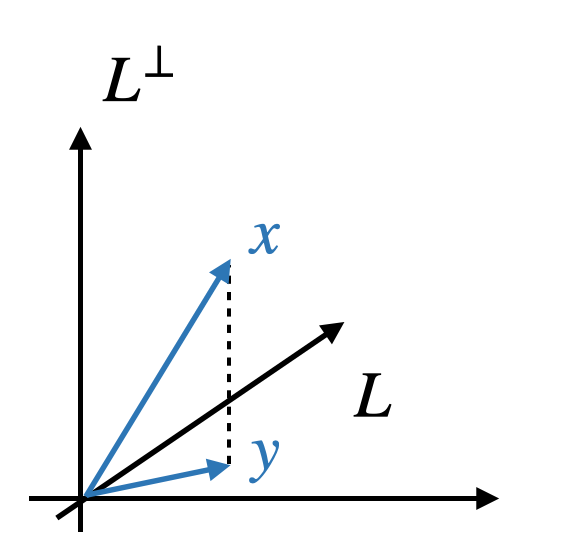
\includegraphics[width=0.2\linewidth]{figs/proj-o.png}
\end{figure}
\end{definition}

\begin{definition}[正交投影矩阵]
正交投影算子 $P_{L}$ 在 $\mathbb C^n$ 的基 $e_1,\ldots,e_n$ 下的矩阵称为正交投影矩阵。
\end{definition}


\begin{theorem}[正交投影与幂等 Hermite]
矩阵 $P$ 为正交投影矩阵的充要条件是 $P$ 为幂等 Hermite 矩阵。
\end{theorem}
\begin{proof}
必要性：若 $P$ 为正交投影矩阵，则根据定理 \ref{thm:proj-idem} 知它是幂等矩阵，于是 $R(I-P)=N(P)$。又 $R(P)\perp N(P)$，所以 $R(P)\perp R(I-P)$，因此对于任意 $x,y\in\mathbb C^n$，有：
\begin{align*}
    x^HP^H(I-P)y=0&\implies P^H(I-P)=0\implies P^H=P^HP\\&\implies P=(P^HP)^H=P^HP=P^H
\end{align*}
即 $P$ 是 Hermite 矩阵。

充分性：若 $P$ 是幂等 Hermite 矩阵，则根据定理 \ref{thm:proj-idem} 知它是投影矩阵 $P_{R(P),N(P)}$.  又由于 $P^H=P$，所以：
\[
    P_{R(P),N(P)}=P_{R(P),N(P^H)}=P_{R(P),R^\perp(P)}
\]
即 $P$ 是正交投影矩阵。
\end{proof}

\noindent\textbf{计算方法}：取 $L$ 的一组基 $X=(x_1,\ldots,x_r)$，$L^{\perp}$ 的一组基 $y=(y_1,\ldots,y_{n-r})$，则 $X^HY=Y^HX=O$.  根据投影矩阵的计算方法知：
\[
    P_L=P_{L,L^\perp}
    =\left[\begin{array}{c:c}X&Y\end{array}\right]\;I_r\;\left[\begin{array}{c:c}X&Y\end{array}\right]^{-1}
    =\left[\begin{array}{c:c}X&O\end{array}\right]\left[\begin{array}{c:c}X&Y\end{array}\right]^{-1}
\]
由于：
\[
    \left[\begin{array}{c:c}X&Y\end{array}\right]^{H}\left[\begin{array}{c:c}X&Y\end{array}\right]=\left[\begin{array}{c}X^H\\\hdashline Y^H\end{array}\right]\left[\begin{array}{c:c}X&Y\end{array}\right]=\left[\begin{array}{c:c}X^HX&O\\\hdashline O&Y^HY\end{array}\right]
\]
于是：
\[
    \left[\begin{array}{c:c}X&Y\end{array}\right]^{-1}=\left[\begin{array}{c:c}(X^HX)^{-1}&O\\\hdashline O&(Y^HY)^{-1}\end{array}\right]\left[\begin{array}{c}X^H\\\hdashline Y^H\end{array}\right]=\left[\begin{array}{c}(X^HX)^{-1}X^H\\\hdashline(Y^HY)^{-1}Y^H\end{array}\right]
\]
因此：
\[
    P_L=\left[\begin{array}{c:c}X&O\end{array}\right]\left[\begin{array}{c:c}X&Y\end{array}\right]^{-1}=\left[\begin{array}{c:c}X&O\end{array}\right]\left[\begin{array}{c}(X^HX)^{-1}X^H\\\hdashline(Y^HY)^{-1}Y^H\end{array}\right]=X(X^HX)^{-1}X^H
\]

\begin{com}
同样的，正交投影矩阵的计算也与选取的基无关。假设有另一组基 $\bar X=(\bar x_1,\ldots,\bar x_r)$，设 $\bar X=XR$，则：
\begin{align*}
    \bar P_L&=\bar X({\bar X}^H\bar X)^{-1}{\bar X}^H=XR(R^HX^HXR)^{-1}R^HX^H\\
    &=XRR^{-1}(X^HX)^{-1}(R^H)^{-1}R^HX^H=X(X^HX)^{-1}X^H=P_L
\end{align*}
可见 $P_L$ 与基的选取无关。
\end{com}

\begin{remark}
由于 $X$ 是列满秩矩阵，根据下一节的内容可知 $X^+=(X^HX)^{-1}X$，所以 $P_L=XX^+$.
\end{remark}


\subsection{广义逆矩阵的存在、性质及构造方法}

\begin{definition}
\label{def:moore-penrose}
设矩阵 $A\in\mathbb C^{m\times n}$，若矩阵 $X\in\mathbb C^{n\times m}$ 满足如下四个 Penrose 方程：
\begin{align*}
    &AXA=A\tag{1}\label{1}\\
    &XAX=X\tag{2}\label{2}\\
    &(AX)^H=AX\tag{3}\label{3}\\
    &(XA)^H=XA\tag{4}\label{4}
\end{align*}
则称 $X$ 为 $A$ 的 Moore-Penrose 逆，记作 $A^+$.
若 $X$ 值满足上述四个方程中的第 $(i),(j),\ldots,(l)$ 个方程，则称 $X$ 为 $A$ 的 $\{i,j,\ldots,l\}$-逆，记作 $A^{(i,j,\ldots,l)}$，其全体记为 $A\{i,j,\ldots,l\}$.

如下为 1-逆的示意图：
\begin{figure}[H]
    \centering
    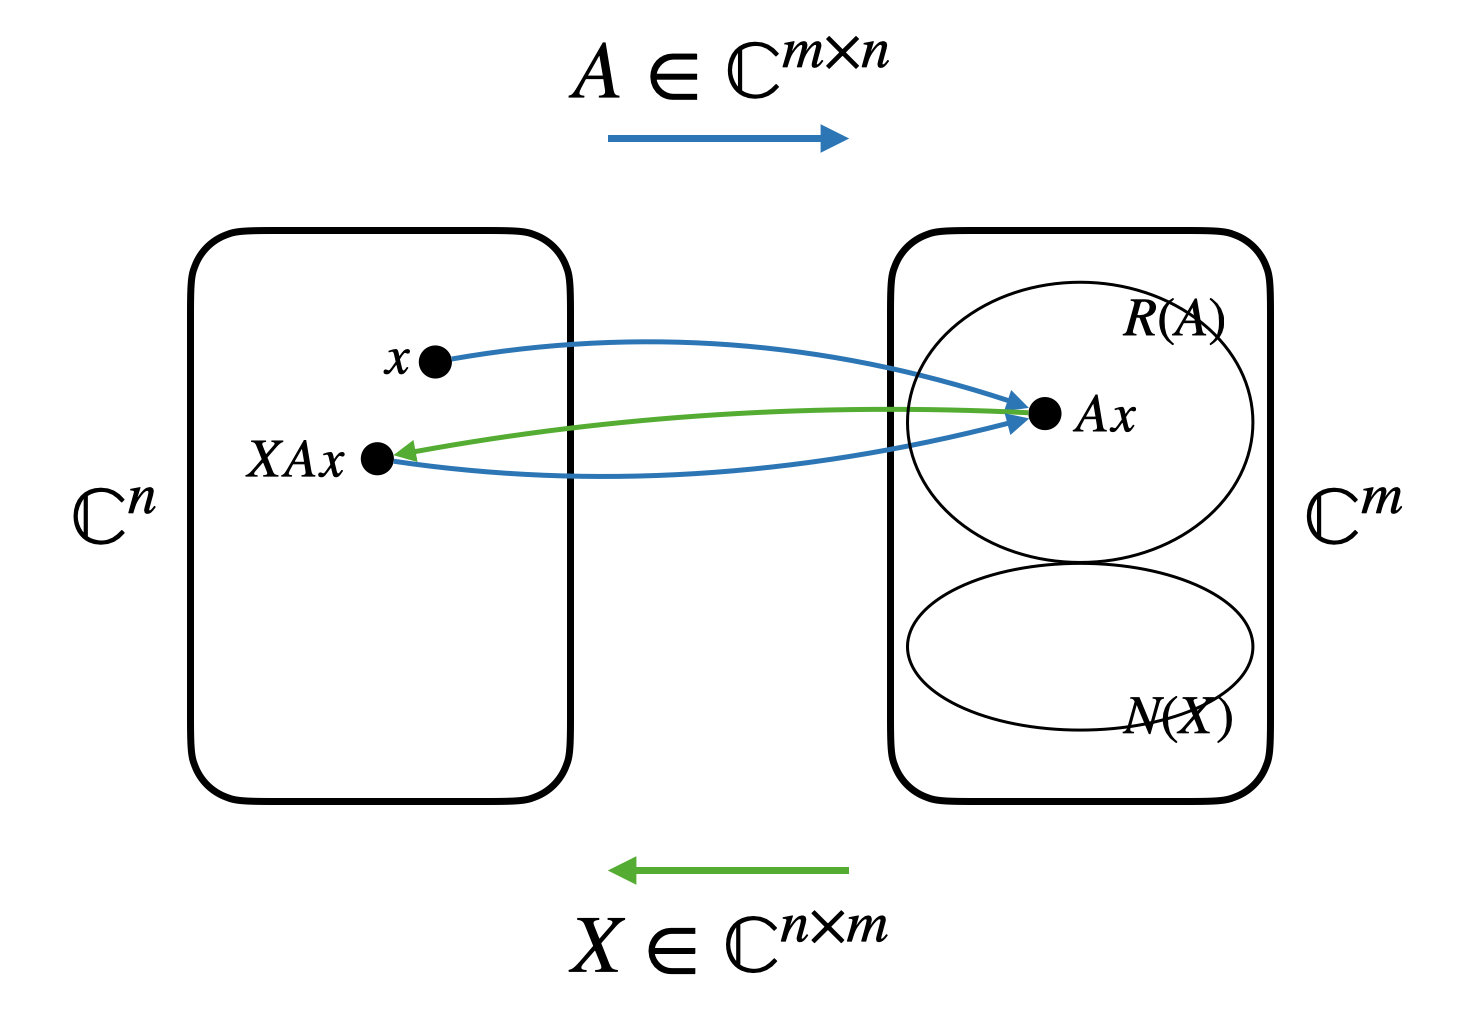
\includegraphics[width=0.5\linewidth]{figs/1inv.png}
\end{figure}
\end{definition}

\begin{theorem}
对任意 $A\in\mathbb C^{m\times n}$，$A^+$ 存在且唯一。
\end{theorem}
\begin{proof}
存在性。对 $A$ 做奇异值分解 $A=U\begin{bmatrix}\Sigma&0\\0&0\end{bmatrix}V^H$，取 $X=V\begin{bmatrix}\Sigma^{-1}&0\\0&0\end{bmatrix}U^H$，可以验证 $X$ 满足 $A^+$ 的四个条件。

唯一性。设 $X,Y$ 均是 $A^+$，则：
\begin{align*}
    Y&=YAY=Y(AY)^H=YY^HA^H=YY^H(AXA)^H\\&=YY^HA^H(AX)^H=Y(AY)^HAX=YAYAX=YAX\\
    X&=XAX=(XA)^HX=A^HX^HX=(AYA)^HX^HX\\&=(YA)^HA^HX^HX=(YA)^H(XA)^HX=(YA)^HXAX=(YA)^HX=YAX
\end{align*}
故 $X=Y$.
\end{proof}

\begin{remark}
上述定理的证明过程也给出了 $A^+$ 的一种基于奇异值分解的计算方法：
\[
    A=U\begin{bmatrix}\Sigma&0\\0&0\end{bmatrix}V^H\implies     A^+=V\begin{bmatrix}\Sigma^{-1}&0\\0&0\end{bmatrix}U^H
\]
\end{remark}

\begin{theorem}
\[
    \lim_{\delta\to0}(\delta^2I+A^HA)^{-1}A^H=A^+
\]
\end{theorem}
\begin{proof}
设 $A=U\begin{bmatrix}\Sigma&0\\0&0\end{bmatrix}V^H$，则 $A^HA=V\begin{bmatrix}\Sigma^2&0\\0&0\end{bmatrix}V^H$，于是：
\[\delta^2I+A^HA=V\begin{bmatrix}\Sigma^2+\delta^2I&0\\0&\delta^2I\end{bmatrix}V^H\]
因此：
\begin{align*}
    (\delta^2I+A^HA)^{-1}A^H&=V\begin{bmatrix}\left[\sigma_i^2+\delta^2\right]_{r\times r}&0\\0&\delta^2I\end{bmatrix}^{-1}V^HA^H\\
    &=V\begin{bmatrix}\left[\dfrac{1}{\sigma_i^2+\delta^2}\right]_{r\times r}&0\\0&\delta^{-2}I\end{bmatrix}(AV)^H\\
    &=V\begin{bmatrix}\left[\dfrac{1}{\sigma_i^2+\delta^2}\right]_{r\times r}&0\\0&\delta^{-2}I\end{bmatrix}\begin{bmatrix}\Sigma&0\\0&0\end{bmatrix}U^H\\
    &=V\begin{bmatrix}\left[\dfrac{\sigma_i}{\sigma_i^2+\delta^2}\right]_{r\times r}&0\\0&0\end{bmatrix}U^H\\
\end{align*}
于是当 $\delta\to0$ 时，
\[
\lim_{\delta\to0}(\delta^2I+A^HA)^{-1}A^H=\lim_{\delta\to0}V\begin{bmatrix}\left[\dfrac{\sigma_i}{\sigma_i^2+\delta^2}\right]_{r\times r}&0\\0&0\end{bmatrix}U^H=V\begin{bmatrix}\Sigma^{-1}&0\\0&0\end{bmatrix}U^H=A^+
\]
\end{proof}

\begin{lemma}
\begin{align*}
    N(A)\supset N(B)&\iff \exists X,A=XB\\
    R(A)\subset R(B)&\iff \exists X,A=BX
\end{align*}
\end{lemma}

\begin{corollary}
\label{cor:rankAB}
\begin{align*}
    &\text{rank}(AB)=\text{rank}(A)\implies \exists X,A=ABX\\
    &\text{rank}(BA)=\text{rank}(A)\implies \exists X,A=XBA
\end{align*}
\end{corollary}
\begin{proof}
由于 $R(AB)\subset R(A)$，且 $\dim R(AB)=\text{rank}(AB)=\text{rank}(A)=\dim R(A)$，故 $R(AB)=R(A)$.  于是 $R(AB)\supset R(A)$，根据引理知 $\exists X,A=ABX$.

类似地，由于 $N(BA)\supset N(A)$，且 $\dim N(BA)=n-\text{rank}(BA)=n-\text{rank}(A)=\dim N(A)$，故 $N(BA)=N(A)$.  于是 $N(BA)\subset N(A)$，根据引理知 $\exists X,A=XBA$.
\end{proof}

\begin{remark}
推论的这两个式子在证明中\textbf{非常常用}，即用更复杂的式子表示简单的矩阵，反而有助于证明。
\end{remark}

\begin{theorem}
矩阵 $A\in\mathbb C^{m\times n}$ 有唯一 1-逆的充要条件为 $A$ 是非奇异矩阵，且该 1-逆就是 $A^{-1}$.
\end{theorem}
\begin{proof}
充分性显然，必要性证明如下。设 $Au=0$，$AXA=A$，那么容易验证 $X'=X+u\cdot[1,0,\ldots,0]$ 也满足 $AX'A=A$，由于 1-逆唯一，故 $u=0$，即 $N(A)=\{0\}$.  类似可以证明 $N(A^H)=\{0\}$，于是 $A$ 列满秩且行满秩，故 $A$ 为可逆方阵。
\end{proof}

\begin{property}[1]
$(A^{(1)})^H\in A^{H}\{1\}$.
\end{property}

\begin{property}[2]
$\lambda^+ A^{(1)}\in(\lambda A)\{1\}$. 其中 $\lambda\in\mathbb C,\,\lambda^{+}=\begin{cases}\lambda^{-1},&\lambda\neq 0\\0,&\lambda=0\end{cases}$.
\end{property}

\begin{property}[3]
若 $S$ 和 $T$ 非奇异，则 $T^{-1}A^{(1)}S^{-1}\in(SAT)\{1\}$.
\end{property}

\begin{property}[4]
$\text{rank}(A^{(1)})\geq \text{rank}(A)$.
\end{property}
\begin{proof}
$\text{rank}(A)=\text{rank}(AA^{(1)}A)\leq\text{rank}(A^{(1)})$.
\end{proof}

\begin{property}[5]
$AA^{(1)}$ 和 $A^{(1)}A$ 均为幂等矩阵且与 $A$ 同秩。
\end{property}
\begin{proof}
$\text{rank}(AA^{(1)})\leq\text{rank}(A)=\text{rank}(AA^{(1)}A)\leq\text{rank}(AA^{(1)})$，故 $\text{rank}(AA^{(1)})=\text{rank}(A)$.
\end{proof}

\begin{property}[6]
$R(AA^{(1)})=R(A),\,N(A^{(1)}A)=N(A),\,R((A^{(1)}A)^H)=R(A^H)$.
\end{property}
\begin{proof}
$R(AA^{(1)})\subset R(A)=R(AA^{(1)}A)\subset R(AA^{(1)})$，故 $R(AA^{(1)})=R(A)$.

类似地，$N(A)\subset N(A^{(1)}A)\subset N(AA^{(1)}A)=N(A)$，故 $N(A^{(1)}A)=N(A)$.
\end{proof}

\begin{property}[7]
$A^{(1)}A=I_n\iff \text{rank}(A)=n$，$AA^{(1)}=I_m\iff \text{rank}(A)=m$.
\end{property}
\begin{proof}
根据性质 5，$\text{rank}(A^{(1)}A)=\text{rank}(A)$，因此必要性：$A^{(1)}A=I_n\implies\text{rank}(A^{(1)}A)=n\implies\text{rank}(A)=n$；充分性：$\text{rank}(A)=n\implies \text{rank}(A^{(1)}A)=n$，即 $A^{(1)}A$ 可逆，又 $A^{(1)}A$ 幂等，故为单位阵。另一个类似。证毕。
\end{proof}

\begin{property}[8]
推论 \ref{cor:rankAB} 的进一步阐述，给出了存在的 $X$ 的具体形式：
\begin{gather*}
    AB(AB)^{(1)}A=A\iff\text{rank}(AB)=\text{rank}(A)\\
    B(AB)^{(1)}AB=B\iff\text{rank}(AB)=\text{rank}(B)
\end{gather*}
\end{property}
\begin{proof}
这里只证明第一行，第二行类似可证。

充分性：根据推论 \ref{cor:rankAB}，存在 $X$ 使得 $A=ABX$，于是 $AB(AB)^{(1)}A=AB(AB)^{(1)}ABX=ABX=A$.

必要性：$\text{rank}(A)\geq\text{rank}(AB)\geq\text{rank}(AB(AB)^{(1)}A)=\text{rank}(A)$，故 $\text{rank}(AB)=\text{rank}(A)$.
\end{proof}

\begin{theorem}
设 $Y,Z\in A\{1\}$，则 $X=YAZ\in A\{1,2\}$.
\end{theorem}
\begin{proof}
$XAX=YAZAYAZ=YAYAZ=YAZ=X$，故 $X\in A\{2\}$. 又 $AXA=AYAZA=AZA=A$，故 $X\in A\{1\}$. 综上，$X\in A\{1,2\}$.
\end{proof}
\begin{proof}[证明 2（利用通解形式，见下文）]
奇异值分解 $A=U\begin{bmatrix}\Sigma&0\\0&0\end{bmatrix}V^H$，则 $Y,Z$ 可分别写作：
\[
    Y=V\begin{bmatrix}\Sigma&C_1\\D_1&E_1\end{bmatrix}U^H,\quad Z=V\begin{bmatrix}\Sigma&C_2\\D_2&E_2\end{bmatrix}U^H
\]
于是：
\[
    X=YAZ=V\begin{bmatrix}B^{-1}&C_1\\D_1&E_1\end{bmatrix}U^HU\begin{bmatrix}B&0\\0&0\end{bmatrix}V^HV\begin{bmatrix}B^{-1}&C_2\\D_2&E_2\end{bmatrix}U^H=V\begin{bmatrix}B^{-1}&C_2\\D_1&D_1BC_2\end{bmatrix}U^H
\]
这正是 1,2-逆的通解形式，故 $X\in A\{1,2\}$.
\end{proof}

\begin{theorem}
给定矩阵 $A$ 和 $X\in A\{1\}$，则 $X\in A\{1,2\}$ 的充要条件是 $\text{rank}(X)=\text{rank}(A)$.
\end{theorem}
\begin{proof}
充分性。由于 $X\in A\{1\}$，故 $A=AXA$，于是 $\text{rank}(A)=\text{rank}(AXA)\leq\text{rank}(XA)\leq\text{rank}(X)=\text{rank}(A)$，故 $\text{rank}(X)=\text{rank}(XA)$. 根据推论，存在 $Y$ 使得 $X=XAY$，于是 $XAX=XAXAY=XAY=X$，故 $X\in A\{2\}$.

必要性。由于 $A=AXA,\,XAX=X$，于是 $\text{rank}(X)=\text{rank}(XAX)\leq\text{rank}(A)=\text{rank}(AXA)\leq\text{rank}(X)$，故 $\text{rank}(X)=\text{rank}(A)$.
\end{proof}

\begin{lemma}
对任意矩阵 $A$ 均有：
\[
    \text{rank}(A^HA)=\text{rank}(A)=\text{rank}(AA^H)
\]
\end{lemma}
\begin{proof}
由于 $A^HAx=0\implies x^HA^HAx=0\implies Ax=0$，所以 $N(A^HA)\subset N(A)$.  又 $N(A^HA)\supset N(A)$，于是 $N(A^HA)=N(A)$，于是 $\text{rank}(A^HA)=\text{rank}(A)$. 另一个类似。
\end{proof}

\begin{theorem}
设有矩阵 $A$，则：
\begin{align*}
    &Y=(A^HA)^{(1)}A^H\in A\{1,2,3\}\\
    &Z=A^H(AA^H)^{(1)}\in A\{1,2,4\}
\end{align*}
\end{theorem}
\begin{proof}
由于 $\text{rank}(A^HA)=\text{rank}(A)=\text{rank}(AA^H)$，根据 1-逆的性质 8 有：
\[
    A=A(A^HA)^{(1)}A^HA,\quad A^H=A^HA(A^HA)^{(1)}A^H
\]
因此：
\begin{align*}
    &AYA=A(A^HA)^{(1)}A^HA=A&\implies Y\in A\{1\}\\
    &YAY=(A^HA)^{(1)}A^HA(A^HA)^{(1)}A^H=(A^HA)^{(1)}A^H=Y&\implies Y\in A\{2\}
\end{align*}
又存在 $X$ 使得 $A=XA^HA$，故：
\begin{align*}
    AY&=A(A^HA)^{(1)}A^H=(XA^HA)(A^HA)^{(1)}(XA^HA)^H\\
    &=XA^HA(A^HA)^{(1)}A^HAX^H=XA^HAX^H
\end{align*}
是 Hermite 矩阵，于是 $Y\in A\{3\}$.
$Z$ 可类似证明。
\end{proof}

\begin{theorem}
\[
    A^+=A^{(1,4)}AA^{(1,3)}
\]
\end{theorem}
\begin{proof}
设 $X=A^{(1,4)}AA^{(1,3)}$，根据关于 1,2-逆的定理知 $X\in A\{1,2\}$. 另外，
\[
    AX=AA^{(1,4)}AA^{(1,3)}=AA^{(1,3)},\quad XA=A^{(1,4)}AA^{(1,3)}A=A^{(1,4)}A
\]
均是 Hermite 矩阵，从而得到结论。
\end{proof}
\begin{proof}[证明 2（利用通解形式，见下文）]
{\color{red}{TODO}}
\end{proof}

\begin{theorem}
给定矩阵 $A\in\mathbb C^{m\times n}$，有：
\begin{enumerate}
    \item $\text{rank}(A^+)=\text{rank}(A)$.
    \item $(A^+)^+=A$.
    \item $(A^H)^+=(A^+)^H,\,(A^T)^+=(A^+)^T$.
    \item $(A^HA)^+=A^+(A^H)^+,\,(AA^H)^+=(A^H)^+A^+$.
    \item $A^+=(A^HA)^+A^H=A^H(AA^H)^+$.
    \item $R(A^+)=R(A^H),\,N(A^+)=N(A^H)$.
\end{enumerate}
\end{theorem}
\begin{proof}
前 5 条都可以通过定义证明。对于第 6 条，根据 1 可知 $\text{rank}(A^+)=\text{rank}(A)=\text{rank}(A^H)$，根据 5 可知 $R(A^+)\subset R(A^H),\,N(A^+)\supset N(A^H)$，于是 $R(A^+)=R(A^H),\,N(A^+)=N(A^H)$.
\end{proof}

\begin{corollary}
若 $A\in\mathbb C_n^{m\times n}$，即列满秩，则 $A^+=(A^HA)^{-1}A^H$；若 $A\in\mathbb C_m^{m\times n}$，即行满秩，则 $A^+=A^H(AA^H)^{-1}$.
\end{corollary}

\begin{corollary}
若 $\alpha\in\mathbb C^n$，且 $\alpha\neq 0$，则 $\alpha^+=(\alpha^H\alpha)^{-1}\alpha^H$，而 $(\alpha^H)^+=(\alpha^+)^H=\alpha(\alpha^H\alpha)^{-1}$.
\end{corollary}

\vskip 6pt \noindent\textbf{广义逆的通解形式}：
设 $A\in\mathbb C^{m\times n}_r$，则存在 $m$ 阶可逆矩阵（或酉矩阵）$P$ 和 $n$ 阶可逆矩阵（或酉矩阵）$Q$ 使得 $A=P\begin{bmatrix}B&0\\0&0\end{bmatrix}Q$，其中 $B$ 为 $r$ 阶可逆矩阵。那么，各广义逆的通解形式如下表所示：

\begin{table}[H]
    \centering
    \label{tab:pseudoinv}
    \begin{tabular}{ll}
    \toprule
    \textbf{广义逆} & \textbf{通解} \\ \midrule
    $X \in A\{1\}$ & $\exists\ C,D,E,\quad\;X=Q^{-1}\begin{bmatrix}B^{-1}&C\\D&E\end{bmatrix}P^{-1}$ \\
    $X \in A\{1,2\}$ & $\exists\ C,D,\quad X=Q^{-1}\begin{bmatrix}B^{-1}&C\\D&DBC\end{bmatrix}P^{-1}$ \\
    $X \in A\{1,3\}$ & $\exists\ D,E,\quad\;X=Q^{-1}\begin{bmatrix}B^{-1}&0\\D&E\end{bmatrix}P^{-1}$ \\
    $X \in A\{1,4\}$ & $\exists\ C,E,\quad\;X=Q^{-1}\begin{bmatrix}B^{-1}&C\\0&E\end{bmatrix}P^{-1}$ \\
    $X \in A\{1,2,3\}$ & $\exists\ D,\quad\;X=Q^{-1}\begin{bmatrix}B^{-1}&0\\D&0\end{bmatrix}P^{-1}$ \\
    $X \in A\{1,2,4\}$ & $\exists\ C,\quad\;X=Q^{-1}\begin{bmatrix}B^{-1}&C\\0&0\end{bmatrix}P^{-1}$ \\
    $X \in A\{1,3,4\}$ & $\exists\ E,\quad\;X=Q^{-1}\begin{bmatrix}B^{-1}&0\\0&E\end{bmatrix}P^{-1}$ \\
    $X \in A\{1,2,3,4\}$ & $X=Q^{-1}\begin{bmatrix}B^{-1}&0\\0&0\end{bmatrix}P^{-1}$ \\ \bottomrule
    \end{tabular}
\end{table}

% |       广义逆        |                             通解                             |
% | :-----------------: | :----------------------------------------------------------: |
% |    $X\in A\{1\}$    | $\exists\ C,D,E,\quad\;X=Q^{-1}\begin{bmatrix}B^{-1}&C\\D&E\end{bmatrix}P^{-1}$ |
% |   $X\in A\{1,2\}$   | $\exists\ C,D,\quad X=Q^{-1}\begin{bmatrix}B^{-1}&C\\D&DBC\end{bmatrix}P^{-1}$ |
% |   $X\in A\{1,3\}$   | $\exists\ D,E,\quad\;X=Q^{-1}\begin{bmatrix}B^{-1}&0\\D&E\end{bmatrix}P^{-1}$ |
% |   $X\in A\{1,4\}$   | $\exists\ C,E,\quad\;X=Q^{-1}\begin{bmatrix}B^{-1}&C\\0&E\end{bmatrix}P^{-1}$ |
% |  $X\in A\{1,2,3\}$  | $\exists\ D,\quad\;X=Q^{-1}\begin{bmatrix}B^{-1}&0\\D&0\end{bmatrix}P^{-1}$ |
% |  $X\in A\{1,2,4\}$  | $\exists\ C,\quad\;X=Q^{-1}\begin{bmatrix}B^{-1}&C\\0&0\end{bmatrix}P^{-1}$ |
% |  $X\in A\{1,3,4\}$  | $\exists\ E,\quad\;X=Q^{-1}\begin{bmatrix}B^{-1}&0\\0&E\end{bmatrix}P^{-1}$ |
% | $X\in A\{1,2,3,4\}$ |  $X=Q^{-1}\begin{bmatrix}B^{-1}&0\\0&0\end{bmatrix}P^{-1}$   |

% 如果 $P,Q$ 是酉矩阵，则 $Q^{-1},P^{-1}$ 写为 $Q^H,P^H$ 即可。
\begin{remark}
与通解形式相对应，称定义 \ref{def:moore-penrose} 中给出的广义逆的定义为方程形式。
做证明时，有时使用方程形式不容易想到思路，而使用通解只需要无脑计算即可。
\end{remark}
\begin{remark}
应用奇异值分解可以使得 $A=U\begin{bmatrix}\Sigma&0\\0&0\end{bmatrix}V^H$，这是上面的特殊情形，因此\textbf{做证明题时直接奇异值分解}就行了。
但是做计算题时，奇异值分解比较麻烦，所以我们不必追求让 $B$ 成为对角矩阵，只需要使得 $B$ 可逆即可。可以通过如下方式计算 $P,Q,B$：
\[
    \begin{bmatrix}A&I_m\\I_n&0\end{bmatrix}\xrightarrow[\text{列变换}]{\text{行变换}}\begin{bmatrix}\begin{bmatrix}B&0\\0&0\end{bmatrix}&P\\Q&0\end{bmatrix}
\]
也可以通过 QR 分解做：首先使用列置换矩阵 $P$ 使得 $AP$ 前 $r$ 列线性无关，则对 $AP$ 做 QR 分解得 $AP=Q_1\begin{bmatrix}R_1&G\\0&0\end{bmatrix}$，其中 $R_1$ 为上三角矩阵。再对 $\begin{bmatrix}R_1^H&0\\G^H&0\end{bmatrix}$ 做 QR 分解得 $\begin{bmatrix}R_1^H&0\\G^H&0\end{bmatrix}=Q_2\begin{bmatrix}R_2&0\\0&0\end{bmatrix}$，其中 $R_2$ 为上三角矩阵。于是：
\[
    AP=Q_1\begin{bmatrix}R_2^H&0\\0&0\end{bmatrix}Q_2^H\implies A=Q_1\begin{bmatrix}R_2^H&0\\0&0\end{bmatrix}Q_2^HP^T
\]
这样得到的 $B$ 是一个下三角矩阵。
\end{remark}

\begin{definition}[广义逆的等价定义]
设 $A\in\mathbb C^{m\times n}$，若矩阵 $X\in\mathbb C^{n\times m}$ 满足 $AX=P_{R(A)},\,XA=P_{R(X)}$，其中 $P_L$ 是空间 $L$ 上的正交投影矩阵，则称 $X$ 为 $A$ 的 Moore 广义逆矩阵。
\end{definition}

\begin{theorem}
Moore 广义逆矩阵和 Penrose 广义逆矩阵是等价的。
\end{theorem}


\subsection{广义逆矩阵的计算方法}

\begin{theorem}[利用 Hermite 标准形计算 1-逆和 1,2-逆]
设 $A\in\mathbb C_r^{m\times n}$，又设 $Q\in\mathbb C_m^{m\times m}$ 和 $P\in\mathbb C_n^{n\times n}$ 使得
\[
    QAP=\begin{bmatrix}I_r&K\\0&0\end{bmatrix}
\]
成立（$P$ 可以只是一个列置换矩阵），则对任意 $L\in\mathbb C^{(n-r)\times (m-r)}$，$n\times m$ 矩阵
\[
    X=P\begin{bmatrix}I_r&0\\0&L\end{bmatrix}Q
\]
是 $A$ 的 1-逆，若令 $L=0$ 则 $X$ 是 $A$ 的 1,2-逆。
\end{theorem}

\begin{remark}
理论基础显然是表 \ref{tab:pseudoinv} 中 1-逆和 1,2-逆的通解形式，不过这里不要求 $K=0$，相应代价就是通解中的 $C,D$ 这里必须是零，也就是说得到的是一种特解。
\end{remark}

\begin{theorem}[满秩分解求广义逆矩阵]
设 $A\in\mathbb C_r^{m\times n}$ 的满秩分解为 $A=FG$，则：
\begin{enumerate}
    \item $G^{(i)}F^{(1)}\in A\{i\},\,i=1,2,4$.
    \item $G^{(1)}F^{(i)}\in A\{i\},\,i=1,2,3$.
    \item $G^{(1)}F^{+}\in A\{1,2,3\}$，$G^{+}F^{(1)}\in A\{1,2,4\}$.
    \item $A^+=G^+F^{(1,3)}=G^{(1,4)}F^+$.
    \item $A^+=G^+F^+=G^H(GG^H)^{-1}(F^HF)^{-1}F^H$.
\end{enumerate}
\end{theorem}

\begin{remark}
由于 $F$ 列满秩、$G$ 行满秩，根据 1-逆的性质 7，有 $F^{(1)}F=GG^{(1)}=I_r$.  利用这一点，由定义即可验证 1 与 2。
3 和 4 可由 1 和 2 得到。5 利用了关于行满秩与列满秩的矩阵的 $A^+$ 公式。
\end{remark}

\begin{theorem}[Zlobec 公式计算 $A^+$]
\[
    A^+=A^H(A^HAA^H)^{(1)}A^H
\]
\end{theorem}
\begin{proof}[证明（利用通解形式）]
设 $A=U\begin{bmatrix}\Sigma&0\\0&0\end{bmatrix}V^H$，则：
\[
    A^HAA^H=V\begin{bmatrix}\Sigma&0\\0&0\end{bmatrix}U^HU\begin{bmatrix}\Sigma&0\\0&0\end{bmatrix}V^HV\begin{bmatrix}\Sigma&0\\0&0\end{bmatrix}U^H=V\begin{bmatrix}\Sigma^3&0\\0&0\end{bmatrix}U^H
\]
于是：
\[
    (A^HAA^H)^{(1)}=U\begin{bmatrix}\Sigma^{-3}&C\\D&E\end{bmatrix}V^H
\]
因此：
\[
    A^H(A^HAA^H)^{(1)}A^H=V\begin{bmatrix}\Sigma&0\\0&0\end{bmatrix}U^HU\begin{bmatrix}\Sigma^{-3}&C\\D&E\end{bmatrix}V^HV\begin{bmatrix}\Sigma&0\\0&0\end{bmatrix}U^H=V\begin{bmatrix}\Sigma^{-1}&0\\0&0\end{bmatrix}U^H
\]
这就是 $A^+$ 的通解形式。
\end{proof}

如果用方程形式去证明，需要一些引理的帮助，显得非常麻烦，这里不做叙述。不过这些引理中有一些值得注意，写在下面。

\begin{theorem}
设 $A\in\mathbb C_r^{m\times n},\,U\in\mathbb C^{n\times p},\,V\in\mathbb C^{q\times m}$，则
\[
    U(VAU)^{(1)}V\in A\{1\}\iff \text{rank}(VAU)=\text{rank}(A)
\]
\end{theorem}
\begin{remark}
这个定理是 1-逆的性质 8 的扩展。回顾性质 8（做了变量替换）：
\begin{align*}
    &AU(AU)^{(1)}A=A\iff\text{rank}(AU)=\text{rank}(A)\\
    &A(VA)^{(1)}VA=A\iff\text{rank}(VA)=\text{rank}(A)
\end{align*}
第一条是在 $A$ 的右边乘上 $U$，第二条是在 $A$ 的左边乘上 $V$，而这个定理左右同时乘了 $V$ 和 $U$.
\end{remark}
\begin{proof}
充分性。由 $\text{rank}(VAU)=\text{rank}(A)$ 知 $R(VAU)=R(AU)=R(A),\,N(VAU)=N(VA)=N(A)$. 故存在 $X,Y$ 使得 $A=AUX=YVA$，于是 $AU(VAU)^{(1)}VA=YVAU(VAU)^{(1)}VAUX=YVAUX=YVA=A$.

必要性：{\color{red}{？？？TODO}}
\end{proof}

\begin{theorem}
对任意矩阵 $A$，满足 $X\in A\{1,2\}$ 和 $R(X)=R(A^H),\,N(X)=N(A^H)$ 的唯一矩阵为 $A^+$.
\end{theorem}

\begin{theorem}[Greville 公式计算 $A^+$]
Greville 公式是计算 $A^+$ 的\textbf{增量}公式。
设 $A\in\mathbb C^{m\times n}$，记 $a_k$ 为 $A$ 的第 $k$ 列，$A_k$ 为 $A$ 的前 $k$ 列构成的子矩阵；又记：
\[
    d_k=A^+_{k-1}a_k,\quad c_k=a_k-A_{k-1}d_k
\]
则：
\[
    A^+_k=\begin{bmatrix}A^+_{k-1}-d_kb_k^H\\b_k^H\end{bmatrix},\quad\text{where}\quad b_k^H=\begin{cases}c_k^+,&c_k\neq 0\\(1+d_k^Hd_k)^{-1}d_k^HA^+_{k-1},&c_k=0\end{cases}
\]
\end{theorem}


\subsection{广义逆矩阵与线性方程组求解}

对于方程组 $Ax=b$，如果 $A$ 非奇异，则 $x=A^{-1}b$ 是唯一解。而在其他情况下，我们希望得到类似的结果。
\begin{itemize}
    \item 如果方程组相容，且其解有无数多个，我们希望求\textbf{极小范数解}，即 $\min_{Ax=b}\Vert x\Vert$；
    \item 如果方程组不相容，即无解，那么我们希望求矛盾方程组的\textbf{最小二乘解}，即 $\min \Vert Ax-b\Vert$；
    \item 一般而言，最小二乘解也不唯一，因此我们希望求\textbf{极小范数最小二乘解}，即 $\min_{\min\Vert Ax-b\Vert}\Vert x\Vert$.
\end{itemize}
\begin{com}
本节所用范数均为 2 范数。
\end{com}

\begin{theorem}[线性方程组的相容性、通解与 1-逆]
\label{thm:compatible}
设 $A\in\mathbb C^{m\times n},\,B\in\mathbb C^{p\times q},\,D\in\mathbb C^{m\times q}$，则矩阵方程 $AXB=D$ 相容的充要条件是：
\[
    AA^{(1)}DB^{(1)}B=D
\]
当方程相容时，通解为：
\[
    X=A^{(1)}DB^{(1)}+Y-A^{(1)}AYBB^{(1)}
\]
其中 $Y\in\mathbb C^{n\times p}$ 为任意矩阵。
\end{theorem}
\begin{proof}
充分性，取 $X=A^{(1)}DB^{(1)}$ 即可；必要性，若 $AXB=D$ 有解，则 $D=AXB=AA^{(1)}AXBB^{(1)}B=AA^{(1)}DB^{(1)}B$.

对于通解，首先显然 $X=A^{(1)}DB^{(1)}+Y-A^{(1)}AYBB^{(1)}$ 是方程的解；其次，若 $X$ 是方程的解，则取 $Y=X$ 即可写作通解形式。
\end{proof}

\begin{corollary}
设 $A\in\mathbb C^{m\times n}$，取 $A^{(1)}\in A\{1\}$，则：
\[
    A\{1\}=\{A^{(1)}+Z-A^{(1)}AZAA^{(1)}\mid Z\in\mathbb C^{n\times m}\}
\]
\end{corollary}
\begin{proof}
任意 $X\in A\{1\}$ 满足矩阵方程 $AXA=A$，代入上述定理的通解形式得：
\begin{align*}
    X&=A^{(1)}AA^{(1)}+Y-A^{(1)}AYAA^{(1)}\\
    &=A^{(1)}AA^{(1)}+A^{(1)}+Z-A^{(1)}A(A^{(1)}+Z)AA^{(1)}&Y=A^{(1)}+Z\\
    &=A^{(1)}+Z+A^{(1)}AA^{(1)}-A^{(1)}AA^{(1)}AA^{(1)}-A^{(1)}AZAA^{(1)}\\
    &=A^{(1)}+Z-A^{(1)}AZAA^{(1)}
\end{align*}
\end{proof}

\begin{theorem}
\label{thm:compatible2}
线性方程组 $Ax=b$ 相容的充要条件是：
\[
    AA^{(1)}b=b
\]
通解为：
\[
    x=A^{(1)}b+(I-A^{(1)}A)y
\]
其中 $y\in\mathbb C^{n}$ 为任意向量。
\end{theorem}
\begin{proof}
在定理 \ref{thm:compatible} 中取 $X=x,\,B=I,\,D=b$ 即可。
\end{proof}

定理 \ref{thm:compatible2} 是给定 $A^{(1)}$ 后求解方程的解，反过来，利用方程的解也可以给出 $A^{(1)}$.

\begin{theorem}
若对于任意满足 $Ax=b$ 相容的 $b$，$x=Xb$ 都是解，则 $X\in A\{1\}$.
\end{theorem}
\begin{proof}
考虑 $Ax=a_i$，其中 $a_i$ 为 $A$ 的列，由于 $x=Xa_i$ 是方程的解，所以 $AXa_i=a_i$，于是 $AXA=A$，故 $X\in A\{1\}$.
\end{proof}

\begin{lemma}[极小范数解]
相容方程组 $Ax=b$ 的极小范数解唯一，且这个唯一解在 $R(A^H)$ 中。
\end{lemma}
\begin{proof}
由于 $R(A^H)=N(A)^\perp$，所以设 $x=y+z$，其中 $y=P_{R(A^H)}x\in R(A^H),\,z=P_{N(A)}x\in N(A)$，于是：
\[
    \Vert x\Vert^2=\Vert y+z\Vert^2=\Vert y\Vert^2+\Vert z\Vert^2\geq \Vert y\Vert^2
\]
由于 $Az=0\implies Ay=b$，即 $y$ 也是方程的解，所以为了让 $x$ 是极小范数解，只能是 $z=0$，因此 $x=y\in R(A^H)$.

唯一性。设 $x'\in R(A^H)$ 且 $Ax'=b$，则 $A(x-x')=0$，即 $x-x'\in N(A)=R^{\perp}(A^H)$.  又 $x-x'\in R(A^H)$，故 $x-x'=0$.
\end{proof}

\begin{lemma}
集合 $A\{1,4\}$ 由矩阵方程 $XA=A^{(1,4)}A$ 的所有解组成，其中 $A^{(1,4)}\in A\{1,4\}$.
\end{lemma}
\begin{proof}
$AXA=AA^{(1,4)}A=A$，所以 $X\in A\{1\}$；$(XA)^H=(A^{(1,4)}A)^H=A^{(1,4)}A=XA$，所以 $X\in A\{4\}$.  综上 $X\in A\{1,4\}$.

另一方面，若 $X\in A\{1,4\}$，则
\begin{align*}
    A^{(1,4)}A&=A^{(1,4)}AXA=(A^{(1,4)}A)^H(XA)^H=A^H(A^{(1,4)})^HA^HX^H\\
    &=(AA^{(1,4)}A)^HX^H=A^HX^H=XA
\end{align*}
即 $X$ 是方程的解。
\end{proof}

\begin{remark}
该定理说明尽管 $A^{(1,4)}$ 不唯一，但是 $A^{(1,4)}A$ 唯一。
\end{remark}

\begin{corollary}
$A^{(1,4)}A=P_{R(A^H)}$.
\end{corollary}

\begin{theorem}
设 $A\in\mathbb C^{m\times n},\,A^{(1,4)}\in A\{1,4\}$，则：
\[
    A\{1,4\}=\{A^{(1,4)}+Z(I-AA^{(1,4)})\mid Z\in\mathbb C^{n\times m}\}
\]
\end{theorem}
\begin{proof}
根据引理，任意 $X\in A\{1,4\}$ 满足方程 $XA=A^{(1,4)}A$，代入通解形式得：
\begin{align*}
    X&=A^{(1,4)}AA^{(1,4)}+Y-YAA^{(1,4)}\\
    &=A^{(1,4)}AA^{(1,4)}+A^{(1,4)}+Z-(A^{(1,4)}+Z)AA^{(1,4)}&Y=A^{(1,4)}+Z\\
    &=A^{(1,4)}+Z+A^{(1,4)}AA^{(1,4)}-(A^{(1,4)}+Z)AA^{(1,4)}\\
    &=A^{(1,4)}+Z(I-AA^{(1,4)})
\end{align*}
\end{proof}

\begin{theorem}[相容方程组的极小范数解与 1,4-逆]
设 $Ax=b$ 相容，则 $x=A^{(1,4)}b$ 为极小范数解；反之，若对于任意 $b\in R(A)$，$x=Xb$ 都是极小范数解，则 $X\in A\{1,4\}$.
\end{theorem}
\begin{proof}
由第一节定理知 $x=A^{(1,4)}b$ 一定是解。设 $Au=b$，则 $x=A^{(1,4)}b=A^{(1,4)}Au=(A^{(1,4)}A)^Hu=A^H(A^{(1,4)})^Hu\in R(A^H)$，于是根据本节引理知 $x$ 为唯一极小范数解。

反之，考虑 $Ax=a_i$，由于 $x=Xa_i$ 是方程的极小范数解，所以 $Xa_i=A^{(1,4)}a_i$，故 $XA=A^{(1,4)}A$，根据引理知 $X\in A\{1,4\}$.
\end{proof}

\begin{lemma}
集合 $A\{1,3\}$ 由矩阵方程 $AX=AA^{(1,3)}$ 的所有解组成，其中 $A^{(1,3)}\in A\{1,3\}$.
\end{lemma}
\begin{proof}
$AXA=AA^{(1,3)}A=A$，故 $X\in A\{1\}$；$(AX)^H=(AA^{(1,3)})^H=AA^{(1,3)}=AX$，故 $X\in A\{3\}$. 综上 $X\in A\{1,3\}$.

另一方面，若 $X\in A\{1,3\}$，则：
\begin{align*}
    AA^{(1,3)}&=AXAA^{(1,3)}=(AX)^H(AA^{(1,3)})^H=X^HA^H(A^{(1,3)})^HA^H\\
    &=X^H(AA^{(1,3)}A)^H=X^HA^H=AX
\end{align*}
即 $X$ 是方程的解。
\end{proof}

\begin{remark}
该定理说明尽管 $A^{(1,3)}$ 不唯一，但是 $AA^{(1,3)}$ 唯一。
\end{remark}

\begin{corollary}
$AA^{(1,3)}=P_{R(A)}$.
\end{corollary}

\begin{theorem}
设 $A\in\mathbb C^{m\times n},\,A^{(1,3)}\in A\{1,3\}$，则：
\[
    A\{1,3\}=\{A^{(1,3)}+(I-A^{(1,3)}A)Z\mid Z\in\mathbb C^{n\times m}\}
\]
\end{theorem}
\begin{proof}
根据引理，任意 $X\in A\{1,3\}$ 满足方程 $AX=AA^{(1,3)}$，代入通解形式得：
\begin{align*}
    X&=A^{(1,3)}AA^{(1,3)}+Y-A^{(1,3)}AY\\
    &=A^{(1,3)}AA^{(1,3)}+A^{(1,3)}+Z-A^{(1,3)}A(A^{(1,3)}+Z)&Y=A^{(1,3)}+Z\\
    &=A^{(1,3)}+Z+A^{(1,3)}AA^{(1,3)}-A^{(1,3)}A(A^{(1,3)}+Z)\\
    &=A^{(1,3)}+(I-A^{(1,3)}A)Z
\end{align*}
\end{proof}

\begin{theorem}[矛盾方程组的最小二乘解与 1,3-逆]
设有方程 $Ax=b$，则 $x=A^{(1,3)}b$ 为最小二乘解；反之，若对于任意 $b$，$x=Xb$ 都是最小二乘解，则 $X\in A\{1,3\}$.
\end{theorem}

\begin{theorem}[法方程]
$x$ 是方程组 $Ax=b$ 的最小二乘解的充要条件为：
\[
    A^HAx=A^Hb
\]
\end{theorem}

\begin{theorem}[矛盾方程组的极小范数最小二乘解与 $A^+$]
$x=A^+b$ 是方程组 $Ax=b$ 的唯一极小范数最小二乘解。反之，若对所有 $b$，$x=Xb$ 都是方程 $Ax=b$ 的极小范数最小二乘解，则 $X=A^+$.
\end{theorem}

\begin{theorem}
若矩阵方程 $AXB=D$ 不相容，则其极小范数最小二乘解，即满足 $\min_{\min \Vert AXB-D\Vert}\Vert X\Vert$ 的唯一解为 $X=A^+DB^+$.
\end{theorem}
\begin{proof}
方程两边同时行拉直：
\[
    \overline{\text{vec}}(AXB)=\overline{\text{vec}}(D)\implies (A\otimes B^T)\overline{\text{vec}}(X)=\overline{\text{vec}}(D)
\]
其极小范数最小二乘解为：
\[
    \overline{\text{vec}}(X)=(A\otimes B^T)^+\overline{\text{vec}}(D)=(A^+\otimes (B^T)^+)\overline{\text{vec}}(D)=(A^+\otimes (B^+)^T)\overline{\text{vec}}(D)
\]
于是反过来应用拉直算子得 $X=A^+DB^+$.
\end{proof}

\begin{com}
上述过程应用了 $(A\otimes B)^+=A^+\otimes B^+$ 的结论，该结论可以通过定义验证。
\end{com}


\vskip 6pt \noindent\textbf{小结}：对于 $Ax=b$，有：
\begin{itemize}
    \item $Ax=b$ 相容的充要条件是 $AA^{(1)}b=b$
    \item 若 $Ax=b$ 相容，则通解为 $x=A^{(1)}b+(I-A^{(1)}A)y$
    \item 若 $Ax=b$ 相容，则极小范数解为 $x=A^{(1,4)}b$
    \item 若 $Ax=b$ 不相容，则最小二乘解为 $x=A^{(1,3)}b$
    \item 若 $Ax=b$ 不相容，则极小范数最小二乘解为 $x=A^+b$
\end{itemize}

对于 $AXB=D$，有：
\begin{itemize}
    \item $AXB=D$ 相容的充要条件是 $AA^{(1)}DB^{(1)}B=D$
    \item 若 $AXB=D$ 相容，则通解为 $X=A^{(1)}DB^{(1)}+Y-A^{(1)}AYBB^{(1)}$
    \item 若 $AXB=D$ 不相容，则极小范数最小二乘解为 $X=A^+DB^+$
\end{itemize}

\vskip 6pt \noindent\textbf{广义逆的集合表示}

\begin{itemize}
    \item $A\{1\}=\{X\mid AXA=A\}=\{A^{(1)}+Z-A^{(1)}AZAA^{(1)}\mid Z\in\mathbb C^{n\times m}\}$
    \item $A\{1,3\}=\{X\mid AX=AA^{(1,3)}\}=\{A^{(1,3)}+(I-A^{(1,3)}A)Z\mid Z\in\mathbb C^{n\times m}\}$
    \item $A\{1,4\}=\{X\mid XA=A^{(1,4)}A\}=\{A^{(1,4)}+Z(I-AA^{(1,4)})\mid Z\in\mathbb C^{n\times m}\}$
    \item $A\{1,2\}=\{X\mid \text{rank}(X)=\text{rank}(A),\,X\in A\{1\}\}$
\end{itemize}
 \newpage

\bibliographystyle{unsrt}
\bibliography{references}

\end{document}
